%!TEX encoding = UTF-8 Unicode
\documentclass[a4paper]{compendium}
%\usepackage{xr} %to crossreference to compendium1.tex
\externaldocument{compendium1}
\usepackage[swedish]{babel}


\addto\captionsswedish{%
  \renewcommand{\appendixname}{Appendix}%
}
%TODO: Glossary
%http://tex.stackexchange.com/questions/5821/creating-a-standalone-glossary/5837#5837

\setlength{\columnsep}{16mm}

\title{
{\vspace{-3.0cm}\bf\sffamily\Huge\selectfont  Introduktion till programmering med Scala}
\\ \vspace{2em}%\hspace*{1.5cm}\inputgraphics[width=0.6\textwidth]{../img/gurka} \\
{\sffamily \textbf{Kompendium 2}\\Andra läsperioden: Modul 8 -- 14}\\\vspace{2cm}
%
\includegraphics[height=4cm]{../img/scala-logo.png}
%
\includegraphics[height=4cm]{../img/java-logo.png}
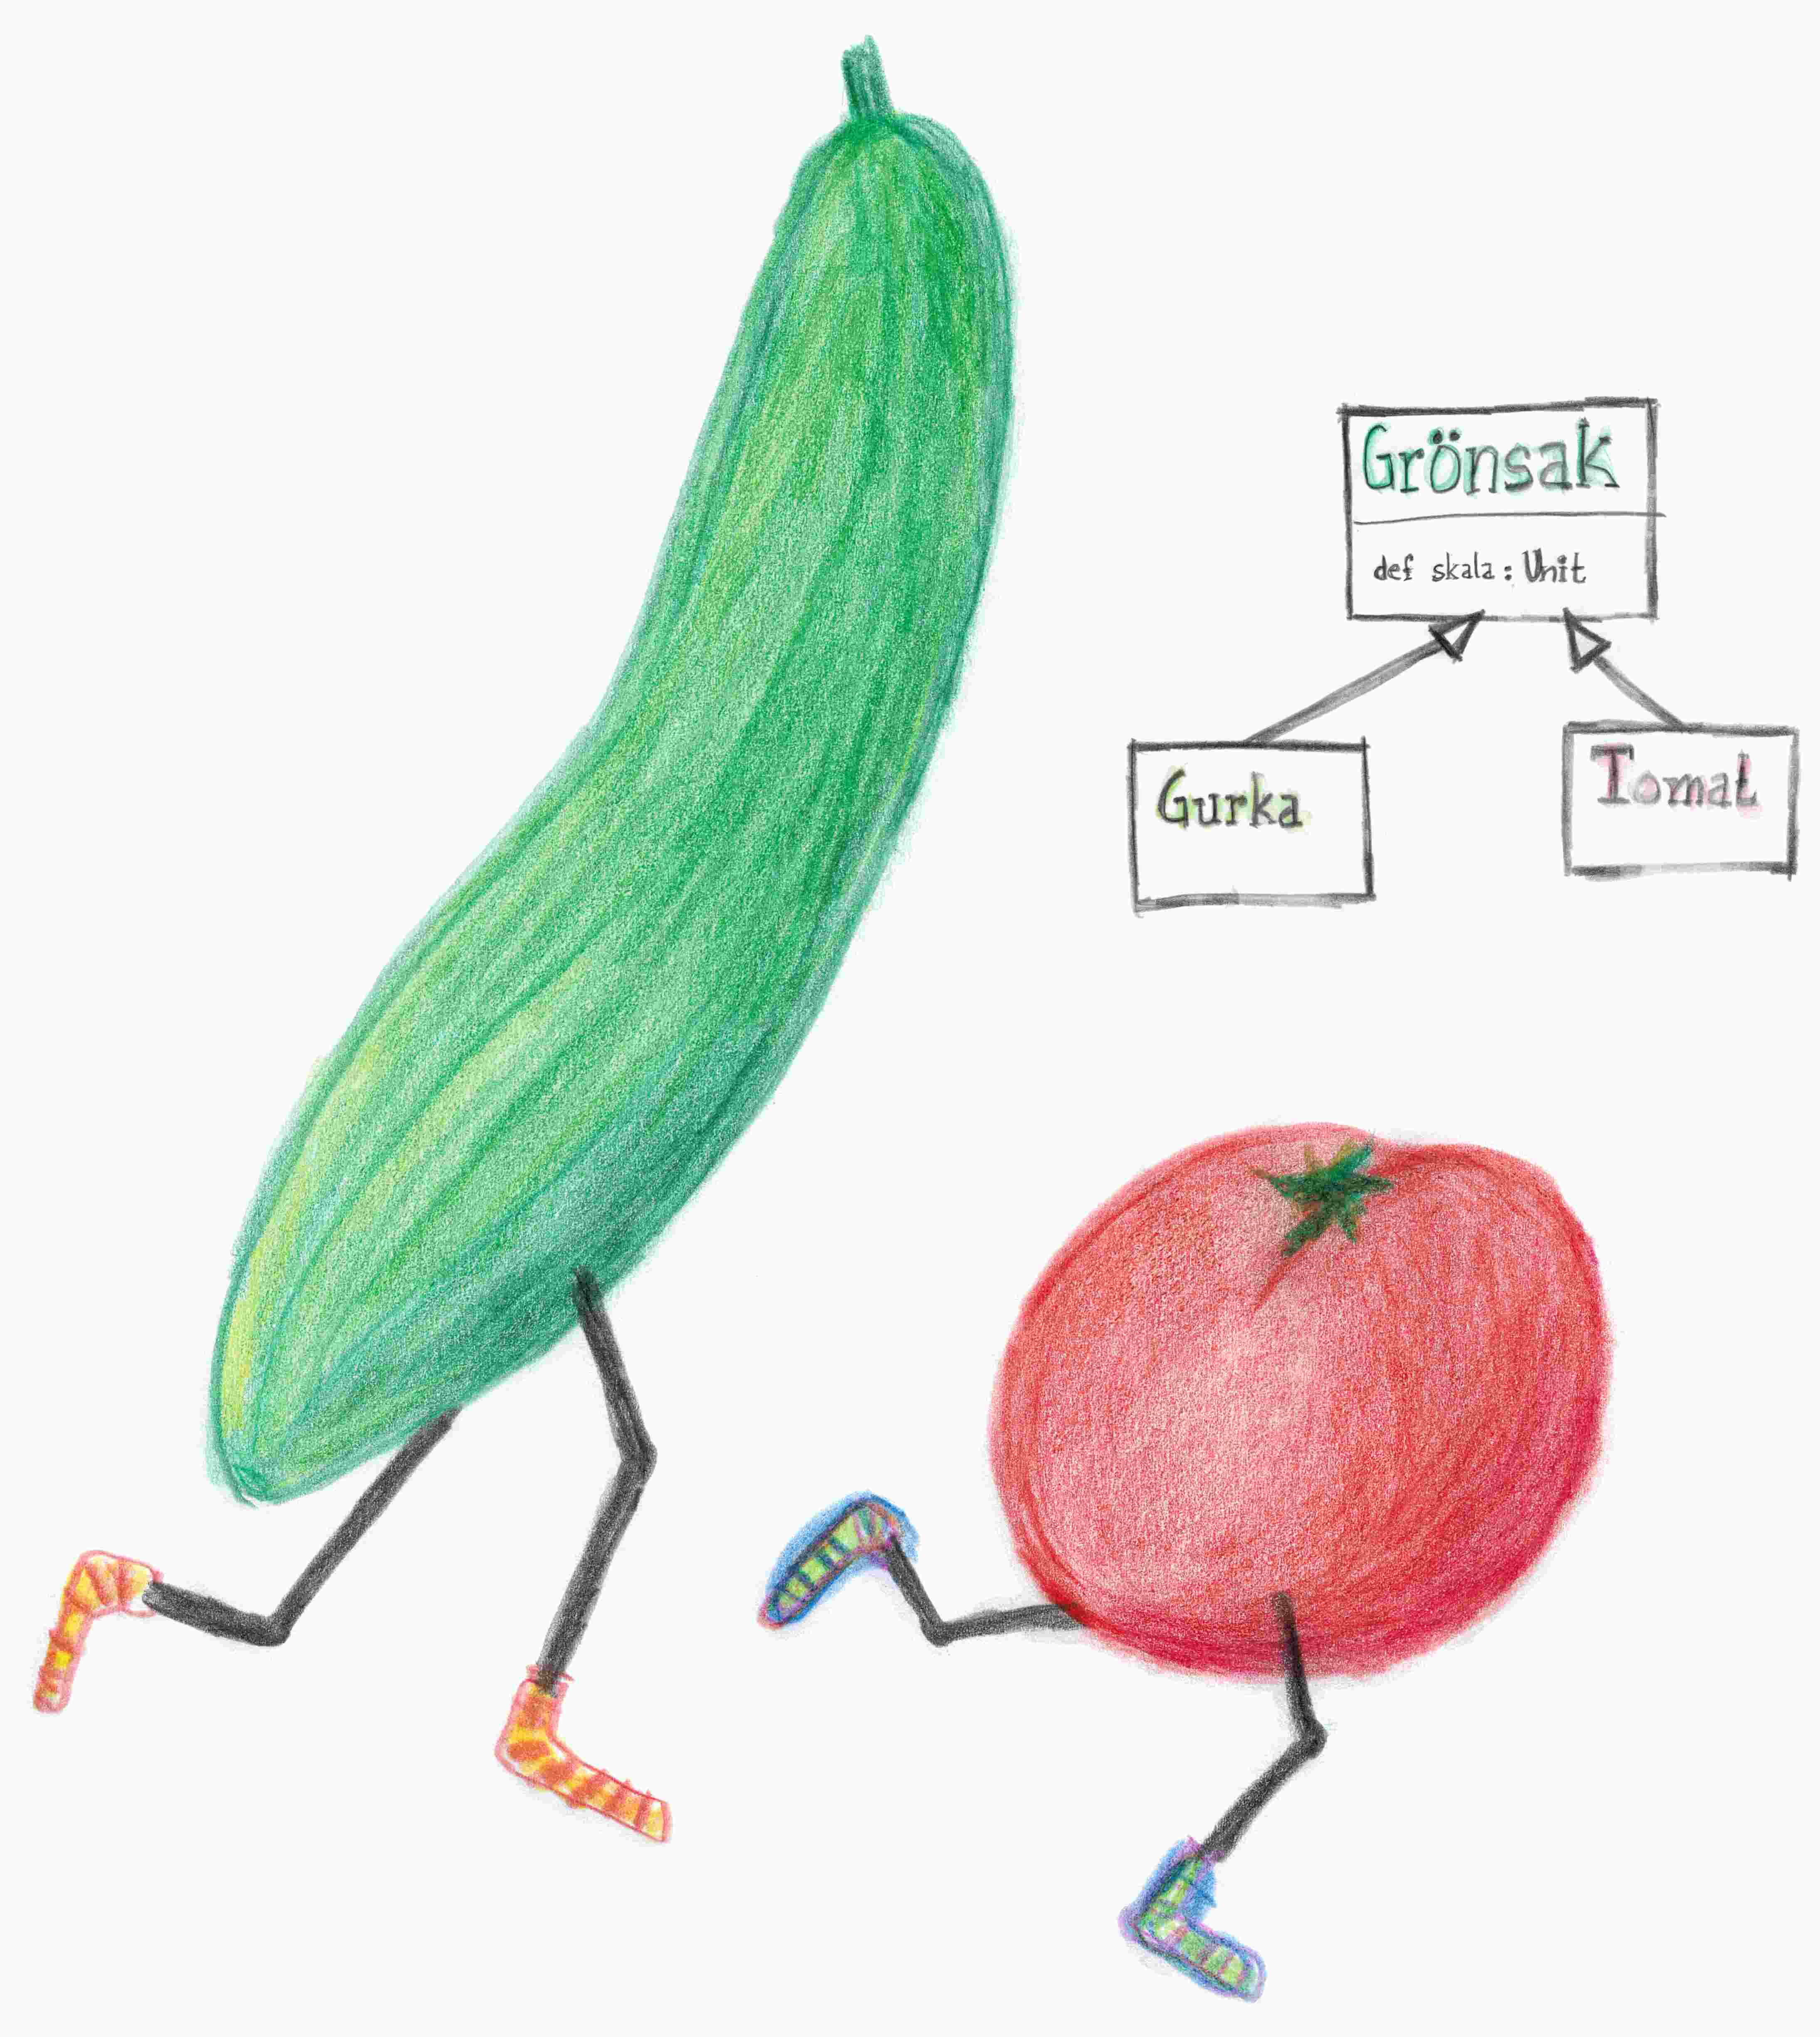
\includegraphics[height=12cm]{cover/gurka.jpg}
}

%\author{Redaktör: Björn Regnell}
\date{\raggedbottom%
\vspace{-2em}\begin{minipage}{1.0\textwidth}\centering
EDAA45, Lp1-2, HT 2016\\
Datavetenskap, LTH\\
Lunds Universitet\\
~\\
Kompileringsdatum: \today \\
\url{http://cs.lth.se/pgk}
\end{minipage}
}

\usepackage{multicol}

\usepackage{pgffor}  %% http://stackoverflow.com/questions/2561791/iteration-in-latex
                     %  allows:  \foreach \n in {1,...,4}{ do something with \n }

\usepackage{framed}  %  allows:   \begin{framed}\end{framed}
%\newenvironment{Slide}[2][]
%  {\begin{framed}\setlist{noitemsep}\section*{#2}}
%  {\end{framed}}

\newcommand{\SlideHeading}[1]{\section*{#1}}

\usepackage[most]{tcolorbox}
\newenvironment{Slide}[2][]
  {\vspace{0.5em}\begin{tcolorbox}[left=1.5em,%width=1.05\textwidth,
  grow to right by=0.05\textwidth,grow to left by=0.05\textwidth,%
  %breakable,
  %frame hidden,
  colframe=gray!20,
  enhanced]\setlist{noitemsep}\SlideHeading{#2}}
  {\end{tcolorbox}\vspace{0.5em}}

\newcommand{\Subsection}[1]{} %ignore slide sections
\newcommand{\SlideOnly}[1]{} %ignore slide font size

\usepackage[framemethod=tikz]{mdframed}

\newif\ifkompendium  % to allow conditional text in slides only showing up in compendium
\kompendiumtrue      % in slides: \kompendiumfalse

\newif\ifPreSolution  % to allow tasks and solutions in same file
\PreSolutiontrue      % in solutions: \PreSolutionfalse

\let\QUESTBEGIN\ifPreSolution  % to mark formatting and numbering of exercises
\let\SOLUTION\else  % to mark solutions in the same file as questions
\let\QUESTEND\fi    % to mark end of exercise

%!TEX encoding = UTF-8 Unicode
\newcommand{\ExeWeekONE}{expressions}
\newcommand{\LabWeekONE}{kojo}

\newcommand{\ExeWeekTWO}{programs}
\newcommand{\LabWeekTWO}{--}

\newcommand{\ExeWeekTHREE}{functions}
\newcommand{\LabWeekTHREE}{blockmole}

\newcommand{\ExeWeekFOUR}{data}
\newcommand{\LabWeekFOUR}{pirates}

\newcommand{\ExeWeekFIVE}{sequences}
\newcommand{\LabWeekFIVE}{shuffle}

\newcommand{\ExeWeekSIX}{classes}
\newcommand{\LabWeekSIX}{turtlegraphics}

\newcommand{\ExeWeekSEVEN}{traits}
\newcommand{\LabWeekSEVEN}{turtlerace-team}

\newcommand{\ExeWeekEIGHT}{matching}
\newcommand{\LabWeekEIGHT}{chords-team}

\newcommand{\ExeWeekNINE}{matrices}
\newcommand{\LabWeekNINE}{maze}

\newcommand{\ExeWeekTEN}{sorting}
\newcommand{\LabWeekTEN}{survey}

\newcommand{\ExeWeekELEVEN}{scalajava}
\newcommand{\LabWeekELEVEN}{lthopoly-team}

\newcommand{\ExeWeekTWELVE}{threads}
\newcommand{\LabWeekTWELVE}{life}

\newcommand{\ExeWeekTHIRTEEN}{Uppsamling}
\newcommand{\LabWeekTHIRTEEN}{Projekt}

\newcommand{\ExeWeekFOURTEEN}{Extenta}
\newcommand{\LabWeekFOURTEEN}{--}



\begin{document}

\pagenumbering{roman}

\frontmatter
\maketitle
%!TEX encoding = UTF-8 Unicode
%!TEX root = ../compendium.tex

\clearpage\null\thispagestyle{empty}
\vfill

{
\setlength{\parindent}{0pt}
\emph{Editor}: Björn Regnell \\ 

%  LIST OF CONTRIBUTORS to https://github.com/lunduniversity/introprog
%    Please contact bjorn.regnell@cs.lth.se if you think you should be 
%    on this list, or make a pull request with an update of file briefly 
%    describing your contribtion in the commit text. 
%    This work is licenced under CC-BY-SA-4.0.
%!TEX encoding = UTF-8 Unicode
%!TEX root = compendium/compendium.tex
\hyphenation{Borg-lund Da-ne-bjer Grampp Palm-qvist Ravn-borg Ro-sen-qvist Schrei-ter Wih-lan-der}
\emph{Contributors} in alphabetical order:
Anders Buhl,
Anna Axelsson,
Anna Palmqvist Sjövall,
Anton Andersson,
Björn Regnell,
Casper Schreiter,
Cecilia Lindskog,
David Söderberg,
Emelie Engström,
Emil Wihlander,
Erik Bjäreholt,
Erik Grampp,
Fredrik Danebjer,
Gustav Cedersjö,
Henrik Olsson,
Jakob Hök,
Johan Ravnborg,
Jonas Danebjer,
Jos Rosenqvist,
Måns Magnusson,
Maj Stenmark,
Oscar Sigurdsson,
Oskar Berg,
Oskar Widmark,
Patrik Persson,
Per Holm,
Sandra Nilsson,
Sebastian Hegardt,
Simon Persson,
Stefan Jonsson,
Tim Borglund,
Tom Postema,
Valthor Halldorsson, 
Viktor Claesson.

\\ \newline

\emph{Home}: \url{https://cs.lth.se/pgk} \newline

\emph{Repo}: \url{https://github.com/lunduniversity/introprog} \\ \newline

This compendium is on-going work. \\ \textbf{Contributions are welcome!} \\ 
\emph{Contact}: \url{bjorn.regnell@cs.lth.se}
\\ \newline

\emph{Cover art}: Björn Regnell (inspired by Poul Ströyer's illustration of Lennart Hellsing's lyrics to  the childrens song ''Herr Gurka'' with music by Knut Brodin)\\ \newline

~\\ \newline

\emph{LICENCE}: CC BY-SA 4.0 \\
\url{http://creativecommons.org/licenses/by-sa/4.0/} \\
Please do \emph{not} distribute your solutions to lab assignments and projects. 
\\ \newline
Copyright \copyright~ 2015-2016. \\
Dept. of Computer Science, LTH, Lund University. Lund. Sweden.\\
}
%!TEX encoding = UTF-8 Unicode
%!TEX root = ../compendium.tex

\ChapterUnnum{Framstegsprotokoll}\label{progress-protocoll} 


\subsubsection*{Genomförda övningar}

\vspace{1em}\noindent 
{Till varje laboration hör en övning med uppgifter som utgör förberedelse inför labben. Du behöver minst behärska grunduppgifterna för att klara labben inom rimlig tid. Om du känner att du behöver öva mer på grunderna, gör då även extrauppgifterna. Om du vill fördjupa dig, gör fördjupningsuppgifterna som är på mer avancerad nivå. Kryssa för nedan vilka övningar du har gjort, så blir det lättare för din handledare att anpassa dialogen till de kunskaper du förvärvat hittills.}

\newcommand{\TickBox}{\raisebox{-.50ex}{\Large$\square$}}
\newcommand{\ExeRow}[1]{\hyperref[section:exe:#1]{\texttt{#1}} & \TickBox  &  \TickBox &  \TickBox  \\ \addlinespace }

\begin{table}[h]
\centering
\vspace{2em}
\begin{tabular}{lccc}
\toprule \addlinespace 
{\sffamily\small Övning} & 
{\sffamily\small Grund} &	
{\sffamily\small Extra} &
{\sffamily\small Fördjupning}\\ \addlinespace \midrule \\[-0.7em]
%!TEX encoding = UTF-8 Unicode
\ExeRow{expressions}
\ExeRow{programs}
\ExeRow{functions}
\ExeRow{data}
\ExeRow{sequences}
\ExeRow{classes}
\ExeRow{traits}
\ExeRow{matching}
\ExeRow{matrices}
\ExeRow{sorting}
\ExeRow{scalajava}
\ExeRow{threads}
\bottomrule
\end{tabular}
\end{table}

\newpage

\subsubsection*{Godkända obligatoriska moment}

\vspace{1em}\noindent 
För att bli godkänd på laborationsuppgifterna och projektuppgiften måste du lösa deluppgifterna och diskutera dina lösningar med en handledare. Denna diskussion är din möjlighet att få feedback på dina lösningar. Ta vara på den!
Se till att handledaren noterar nedan när du blivit godkänd på respektive labb. Spara detta blad tills du fått slutbetyg i kursen. 


\vspace{2.5em}\noindent Namn: \dotfill\\

\vspace{1em}\noindent Namnteckning: \dotfill\\

\newcommand{\LabRow}[1]{\\[-1.1em] \hyperref[section:lab:#1]{\texttt{#1}} & \dotfill &  \dotfill  \\ \addlinespace }

\begin{table}[h]
\centering
\vspace{1em}
\begin{tabular}{lcc}
\toprule \addlinespace 
{\sffamily\bfseries\small Lab} & {\sffamily\small Datum gk} &	{\sffamily\small Handledares namnteckning}\\ \addlinespace \midrule \\[-0.5em]
%!TEX encoding = UTF-8 Unicode
\LabRow{kojo}
\LabRow{blockmole}
\LabRow{pirates}
\LabRow{shuffle}
\LabRow{turtlegraphics}
\LabRow{turtlerace-team}
\LabRow{chords-team}
\LabRow{maze}
\LabRow{surveydata}
\LabRow{lthopoly-team}
\LabRow{life}
\LabRow{Projekt}
%\toprule 
\addlinespace \midrule \addlinespace
{\sffamily\small {\bfseries Projektuppgift} (välj en)	} & 
\multicolumn{2}{c}{\textit{Om egendef., ge kort beskrivning:}}  \\ 
\addlinespace\addlinespace %\midrule
{\Large$\square$}\texttt{~~~\hyperref[section:proj:bank]{bank}}  &  &  \\
{\Large$\square$}\texttt{~~~\hyperref[section:proj:imageprocessing]{imageprocessing}}  \\
{\Large$\square$}\texttt{~~~\hyperref[section:proj:tictactoe]{tictactoe}} \\  
{\Large$\square$}\texttt{~~~}\textit{egendefinerad}  \\
\\
\\
%\dotfill  \\
\bottomrule
\end{tabular}
\end{table}
%!TEX encoding = UTF-8 Unicode
%!TEX root = ../compendium1.tex


\ChapterUnnum{Förord}

Detta kompendium innehåller övningar och laborationer och övningslösningar för andra läsperioden i LTH:s grundkurs i programmering för civilingenjörsprogrammet Datateknik.


Vi avslutade första läsperioden med en diagnostisk kontrollskrivning där du fick återkoppling på vad du lärt dig hittills. Det är viktigt att du använder dina lärdomar om vad du behöver träna mer på och direkt gör upp en plan för hur du kan befästa din förståelse för begreppen i första läsperioden, så att du hänger med under kommande läsperiod.

Det övergripande målet för den andra läsperioden är att du ska kunna skapa egna program som löser mer omfattande problem än tidigare, genom att kombinera flera abstraktionsmekanismer och begrepp. Vi inför även nya abstraktionsmekanismer (t.ex. arv), nya språkmekanismer (t.ex. mönstermatching), samt jämför och kombinerar Scala och Java. Läsperioden avslutas med ett individuellt projektarbete där du får möjlighet att fördjupa dig enligt dina egna intressen och önskemål.

Kompendiet är framtaget för och av studenter och lärare, och distribueras som öppen källkod. Det får användas fritt så länge erkännande ges och eventuella ändringar publiceras under samma licens som ursprungsmaterialet. På kurshemsidan \href{http://cs.lth.se/pgk}{cs.lth.se/pgk} och i kursrepot \href{http://github.com/lunduniversity/introprog}{github.com/lunduniversity/introprog} finns instruktioner om hur du kan bidra till kursmaterialet.

Välkommen till andra halvlek!

\vspace{1em}\noindent \textit{\hfill Lund, \today, Björn Regnell}


\setcounter{tocdepth}{2} % set headings level in table of contents
\tableofcontents
\mainmatter

\pagenumbering{arabic}


\part{Modulöversikt}

\begin{table}
\noindent\resizebox{1.0\columnwidth}{!}{
\renewcommand{\arraystretch}{2.0}
%!TEX encoding = UTF-8 Unicode
\begin{tabular}{l|l|l|l}
\textit{W} & \textit{Modul} & \textit{Övn} & \textit{Lab} \\ \hline \hline
W01 & Introduktion            & expressions & kojo            \\
W02 & Kodstrukturer           & programs    & --              \\
W03 & Funktioner, Objekt      & functions   & simplewindow    \\
W04 & Datastrukturer          & data        & textfiles       \\
W05 & Sekvensalgoritmer       & sequences   & cardgame        \\
W06 & Klasser, Likhet         & classes     & shapes          \\
W07 & Arv, Gränssnitt         & traits      & turtlerace-team \\
KS  & KONTROLLSKRIVN.         & --          & --              \\
W08 & Mönster, Undantag       & matching    & chords-team     \\
W09 & Matriser, Typparametrar & matrices    & maze            \\
W10 & Sökning, Sortering      & sorting     & surveydata-team \\
W11 & Scala och Java          & scalajava   & scalajava-team  \\
W12 & Trådar                  & threads     & life            \\
W13 & Design                  & Uppsamling  & Inl.Uppg.       \\
W14 & Tentaträning            & Extenta     & --              \\
T   & TENTAMEN                & --          & --              \\
\end{tabular}

}
\end{table}
\clearpage

\hyphenation{intro-duktion sekvens-algoritmer kod-strukturer data-strukturer}
{\fontsize{11}{12}\selectfont
\renewcommand{\arraystretch}{1.75}
\begin{longtable}{@{}p{.05\textwidth} | >{\hspace{0.1em}\raggedright\bfseries\sffamily}p{.15\textwidth}  >{\raggedleft\arraybackslash\hspace{0.0em}%\fontsize{10.5}{12}\selectfont
}p{0.735\textwidth}}
W01 & Introduktion & sekvens, alternativ, repetition, abstraktion, programmeringsspråk, programmeringsparadigmer, editera-kompilera-exekvera, datorns delar, virtuell maskin, REPL, literal, värde, uttryck, identifierare, variabel, typ, tilldelning, namn, val, var, def, inbyggda grundtyper, Int, Long, Short, Double, Float, Byte, Char, String, println, typen Unit, enhetsvärdet (), stränginterpolatorn s, if, else, true, false, MinValue, MaxValue, aritmetik, slumptal, math.random, logiska uttryck, de Morgans lagar, while-sats, for-sats \\
W02 & Kodstrukturer & iterering, for-uttryck, map, foreach, Range, Array, Vector, algoritm vs implementation, pseudokod, algoritm: SWAP, algoritm: SUM, algoritm: MIN/MAX, algoritm: MININDEX, block, namnsynlighet, namnöverskuggning, lokala variabler, paket, import, filstruktur, jar, dokumentation, programlayout, JDK, main i Java vs Scala, java.lang.System.out.println \\
W03 & Funktioner, objekt & definera funktion, anropa funktion, parameter, returtyp, värdeandrop, namnanrop, default-argument, namngivna argument, applicera funktion på alla element i en samling, procedur, värdeanrop vs namnanrop, uppdelad parameterlista, skapa egen kontrollstruktur, objekt, modul, punktnotation, tillstånd, metod, medlem, funktionsvärde, funktionstyp, äkta funktion, stegad funktion, apply, lazy val, lokala funktioner, anonyma funktioner, lambda, aktiveringspost, anropsstacken, objektheapen, rekursion  cslib.window.SimpleWindow \\
W04 & Datastrukturer & attribut (fält), medlem, metod, tupel, klass, Any, isInstanceOf, toString, case-klass, samling, scala.collection, föränderlighet vs oföränderlighet, List, Vector, Set, Map, typparameter, generisk samling som parameter, översikt samlingsmetoder, översikt strängmetoder, läsa/skriva textfiler, Source.fromFile, java.nio.file \\
W05 & Sekvensalgoritmer & sekvensalgoritm, algoritm: SEQ-COPY, in-place vs copy, algoritm: SEQ-REVERSE, algoritm: SEQ-REGISTER, sekvenser i Java vs Scala, for-sats i Java, java.util.Scanner, scala.collection.mutable.ArrayBuffer, StringBuilder, java.util.Random, slumptalsfrö \\
W06 & Klasser & objektorientering, klass, Point, Square, Complex, new, null, this, inkapsling, accessregler, private, private[this], kompanjonsobjekt, getters och setters, klassparameter, primär konstruktor, objektfabriksmetod, överlagring av metoder, referenslikhet vs strukturlikhet, eq vs == \\
W07 & Arv & arv, polymorfism, trait, extends, asInstanceOf, with, inmixning, supertyp, subtyp, bastyp, override, klasshierarkin i Scala: Any AnyRef Object AnyVal Null Nothing, referenstyper vs värdetyper, klasshierarkin i scala.collection, Shape som bastyp till Rectangle och Circle, accessregler vid arv, protected, final, klass vs trait, abstract class, case-object, typer med uppräknade värden \\
KS & \multicolumn{2}{l}{KONTROLLSKRIVN.} \\
W08 & Repetition, trösklar, luckor & REBOOT CAMP: identifiera dina egna lärandetrösklar och kunskapsluckor, kom-i-kapp med övningar och labbar, repetera, fördjupning för de som är redo, specialträning för behövande \\
W09 & Mönster, undantag & mönstermatchning, match, Option, throw, try, catch, Try, unapply, sealed, flatten, flatMap, partiella funktioner, collect, speciella matchningar: wildcard pattern; variable binding; sequence wildcard; back-ticks, equals, hashcode, exempel: equals för klassen Complex, switch-sats i Java \\
W10 & Matriser, typparametrar & matris, nästlad samling, nästlad for-sats, typparameter, generisk funktion, generisk klass, fri vs bunden typparameter, matriser i Java vs Scala, allokering av nästlade arrayer i Scala och Java \\
W11 & Sökning, sortering & strängjämförelse, compareTo, implicit ordning, linjärsökning, binärsökning, algoritm: LINEAR-SEARCH, algoritm: BINARY-SEARCH, algoritmisk komplexitet, sortering till ny vektor, sortering på plats, insättningssortering, urvalssortering, algoritm: INSERTION-SORT, algoritm: SELECTION-SORT, Ordering[T], Ordered[T], Comparator[T], Comparable[T] \\
W12 & Scala och Java & syntaxskillnader mellan Scala och Java, klasser i Scala vs Java, referensvariabler vs enkla värden i Java, referenstilldelning vs värdetilldelning i Java, alternativ konstruktor i Scala och Java, for-sats i Java, for-each-sats i Java, java.util.ArrayList, autoboxing i Java, primitiva typer i Java, wrapperklasser i Java, samlingar i Java vs Scala, scala.collection.JavaConverters, namnkonventioner för konstanter \\
W13 & Extra: design, api, trådar, webb & utvecklingsprocessen, krav-design-implementation-test, gränssnitt, trait vs interface, programmeringsgränssnitt (api), designexempel, tråd, jämlöpande exekvering, icke-blockerande anrop, callback, java.lang.Thread, java.util.concurrent.atomic.AtomicInteger, scala.concurrent.Future, kort om html+css+javascript+scala.js och webbprogrammering \\
W14 & \multicolumn{2}{l}{Tentaträning} \\
T & \multicolumn{2}{l}{TENTAMEN} \\
\end{longtable}
}

%\renewcommand{\SlideHeading}[1]{\subsection{#1}}  %numbering sections in compendium slides

\part{Moduler}

\setcounter{chapter}{7}

%\input{modules/w08-matrices-chapter.tex}
%!TEX encoding = UTF-8 Unicode
\chapter{Mönster, undantag}\label{chapter:W08}
Begrepp du ska lära dig denna vecka:
\begin{itemize}[noitemsep,label={$\square$},leftmargin=*]
\item mönstermatchning
\item match
\item Option
\item try
\item catch
\item finally ???
\item Try
\item unapply
\item sealed
\item switch-sats i Java
\item flatten
\item flatMap
\item partiella funktioner
\item collect
\item implementera equals utan arv för Complex
\item implementera equals med arv för Shape ???\end{itemize}

%!TEX encoding = UTF-8 Unicode

%!TEX root = ../compendium2.tex

\Exercise{\ExeWeekEIGHT}\label{exe:W08}

\begin{Goals}
\item Kunna skapa och använda matriser med nästlade strukturer av \code{Vector}.
\item Kunna iterera över elementen i en matris med nästlade \code{for}-satser och \code{for}-\code{yield}-uttryck, samt nästlad applicering av \code{map} respektive \code{foreach}.
\item Kunna skapa och använda funktioner som tar matriser som parametrar.
\item Känna till generiska funktioner.
\item Känna till generiska klasser.
\item Kunna skapa och använda matriser med hjälp inbyggda arrayer i Java.
\item Kunna använda nästlade \code{for}-satser i Java för att iterera över elementen i en matris.
\end{Goals}

\begin{Preparations}
\item \StudyTheory{08}
\end{Preparations}

\BasicTasks %%%%%%%%%%%%%%%%

\Task \emph{Skapa matriser med hjälp av nästlade samlingar.} Man kan i ett datorprogram, med hjälp av samlingar som innehåller samlingar, skapa nästlade strukturer som kan indexeras i två dimensioner och på så sätt representera en matematisk \textbf{matris}.\footnote{\href{https://sv.wikipedia.org/wiki/Matris}{sv.wikipedia.org/wiki/Matris}}
\begin{Background}
En \textbf{matris} inom matematiken innehåller ett antal rader och kolumner (även kallade kolonner). I en matematisk matris har alla rader lika många element och även alla kolumner har lika många element. En matris av dimension $m\times{}n$ har $m \cdot n$ stycken element, där $m$ är antalet rader och $n$ är antalet kolumner. En matris $A_{m,n}$ av dimension $m\times{}n$ ritas ofta så här:

\[
A_{m,n} =
 \begin{pmatrix}
  a_{1,1} & a_{1,2} & \cdots & a_{1,n} \\
  a_{2,1} & a_{2,2} & \cdots & a_{2,n} \\
  \vdots  & \vdots  & \ddots & \vdots  \\
  a_{m,1} & a_{m,2} & \cdots & a_{m,n}
 \end{pmatrix}
\]

\noindent Exempel: En heltalsmatris $M_{2,5}$ av dimension $2\times{}5$ där element $m_{2,5}=7$:

\[
M=
  \begin{pmatrix}
    5 & 2 & 42 & 4 & 5 \\
    3 & 4 & 18 & 6 & 7
  \end{pmatrix}
\]
\end{Background}

\Subtask\Pen Rita minnessituationen efter tilldelningen på rad 1 nedan. Vad har \code{m} för typ och värde? Vad har \code{m} för dimensioner? Hur sker indexeringen i ett datorprogram jämfört med i matematiken?

\begin{REPL}
scala> val m = Vector((1 to 5).toVector, (3 to 7).toVector)
scala> m.apply(0).apply(1)
scala> m(1)
scala> m(1)(4)
\end{REPL}

\Subtask Vad ger uttrycken på raderna 2, 3 och 4 ovan för värden och typ?

\Subtask Man kan i ett datorprogram mycket väl skapa tvådimensionella, nästlade strukturer där raderna \emph{inte} innehåller samma antal element. Det blir då ingen äkta matris i strikt matematisk mening, men man kallar ofta ändå en sådan struktur för en ''matris''. Vilken typ har variablerna \code{m2}, \code{m3}, \code{m4} och \code{m5} nedan?

\begin{REPL}
scala> val m2 = Vector(Vector(1,2,3),Vector(4,5),Vector(42))
scala> val m3 = Vector(Vector(1,2), Vector(1.0, 2.0, 3.0))
scala> m3(1)
scala> val m4 = m3(1) +: Vector("a") +: m3
scala> val m5 = Vector.fill(42){ m2(1).map(e => (e * math.random).toInt) }
\end{REPL}

\Subtask\Pen Rita minnessituationen efter tilldelingen av \code{m2} på rad 1 ovan.

\Subtask\Pen Vilken av variablerna \code{m2}, \code{m3}, \code{m4} och \code{m5} ovan representerar en äkta matris i matematisk mening? Vilken är dess dimensioner?



\Task \emph{Skapa och iterera över matriser.} Vi ska skapa matriser där varje rad representerar 5 kast med en tärning i spelet Yatzy.\footnote{\href{https://sv.wikipedia.org/wiki/Yatzy}{sv.wikipedia.org/wiki/Yatzy}}


\Subtask Definiera i REPL en funktion \code{def throwDie: Int = ???} som returnerar ett slumptal mellan 1 och 6.


\Subtask Skapa nedan heltalsmatris i REPL. Vilken dimension får matrisen?
\begin{REPL}
val ds1 = for (i <- 1 to 1000) yield {
            for (j <- 1 to 5) yield throwDice
          }
\end{REPL}

\Subtask\Pen Man kan också använda nedan varianter för att skapa en heltalsmatris. Vilken av varianterna \code{ds1} ... \code{ds5} tycker du är lättast att läsa och förstå? Prova respektive variant i REPL och ange vilken typ på \code{ds1} ... \code{ds5} som härleds av kompilatorn.
\begin{REPL}
val ds2 = (1 to 1000).map(i => (1 to 5).map(j => throwDice))
val ds3 = (1 to 1000).map(i => Vector.fill(5)(throwDice))
val ds4 = for (i <- 1 to 1000) yield Vector.fill(5)(throwDice)
val ds5 = Vector.fill(1000)(Vector.fill(5)(throwDice))
\end{REPL}


\Subtask Definiera en funktion \\ \code{def roll(n: Int): Vector[Int] = ???}\\ som ger en heltalsvektor med $n$ stycken slumpvisa tärningskast. Kasten ska vara sorterade i växande ordning; använd för detta ändamål samlingsmetoden \code{sorted}.



\Subtask Definera i REPL en funktion \code{isYatzy(xs: Vector[Int]): Boolean = ???} som testar om alla elementen i en heltalsvektor är samma. Använd samlingsmetoden \code{forall}.


\Subtask Implementera \code{isYatzy} igen med ett imperativt angreppssätt som använder en \code{while}-sats (alltså utan att använda funktionella  \code{forall}). Ta hjälp av en variabel \code{i} som håller reda på index och en variabel \code{foundDiff} som håller reda på om ett avvikande värde upptäcks. Funktionen blir ca 10 rader, så det kan vara lämpligt att öppna en editor att skriva i medan du klurar ut lösningen. Börja med att skriva pseudokod, gärna med penna på papper. Prova genom att klistra in i REPL.



\Subtask Skapa en funktion  \\ \code{def diceMatrix(m: Int, n: Int): Vector[Vector[Int]] = ???} \\ som med hjälp av funktionen \code{roll} skapar en matris med \code{m} st vektorer med vardera \code{n} slumpvisa tärningskast.


\Subtask Skapa en funktion som returnerar en utskriftsvänlig sträng \\ \code{def diceMatrixToString(xss: Vector[Vector[Int]]): String = ???} \\med hjälp av \code{map} och \code{mkString}, som fungerar enligt nedan.
\begin{REPL}
scala> println(diceMatrixToString(diceMatrix(10, 5)))
4 5 5 3 3
1 4 1 3 1
1 3 1 5 5
6 4 4 5 5
2 1 5 6 5
1 2 2 3 6
1 3 2 4 5
2 2 3 2 2
2 6 3 4 6
4 5 5 2 3

\end{REPL}



\Subtask\Pen Ett imperativt sätt\footnote{Imperativa anreppssätt är nödvändiga att kunna när du stöter på samlingar och/eller språk som saknar funktionsprogrammeringsmöjligheter med \code{map}, \code{mkString} etc.} att göra detta på visas nedan. Förklara hur nedan kod fungerar. Vad händer om \code{xss} är tom? Vad händer om \code{xss} bara innehåller tomma vektorer? Nämn en fördel och en nackdel med att använda \code{val sb: StringBuilder} och \code{append}, jämfört med en vanlig \code{var s: String} och \code{+} för tillägg i slutet.
\begin{Code}
def diceMatrixToString(xss: Vector[Vector[Int]]): String = {
  val sb = new StringBuilder()
  for(m <- 0 until xss.size) {
    for(n <- 0 until xss(m).size) {
      sb.append(xss(m)(n))
      if (n < xss(m).size - 1) sb.append(" ")
      else if (m < xss.size - 1) sb.append("\n")
    }
  }
  sb.toString
}
\end{Code}

\Subtask Implementera funktionen \\ \code{def filterYatzy(xss: Vector[Vector[Int]]): Vector[Vector[Int]]} \\ som filtrerar fram alla yatzy-rader i matrisen \code{xss} enligt nedan. Använd din funktion \code{isYatzy} och samlingsmetoden \code{filter}.
\begin{REPL}
scala> println(diceMatrixToString(filterYatzy(diceMatrix(10000, 5))))
2 2 2 2 2
3 3 3 3 3
1 1 1 1 1
3 3 3 3 3
4 4 4 4 4
6 6 6 6 6
2 2 2 2 2
3 3 3 3 3
2 2 2 2 2
6 6 6 6 6
4 4 4 4 4
2 2 2 2 2
4 4 4 4 4

\end{REPL}



\Subtask Gör som träning en imperativ implementation av \code{filterYatzy} med en \code{for}-sats (alltså utan att använda \code{filter}, och utan att använda \code{yield}).


\Subtask\Pen Tycker du din imperativa lösning är lättare eller svårare att läsa och förstå jämfört nedan funktionella lösning med ett \code{for}-uttryck och \code{yield}?
\begin{CodeSmall}
def filterYatzy(xss: Vector[Vector[Int]]): Vector[Vector[Int]] = {
  for (i <- 0 until xss.size if isYatzy(xss(i))) yield xss(i)
}.toVector
\end{CodeSmall}

\Subtask Implementera funktionen \\
\code{def yatzyPips(xss: Vector[Vector[Int]]): Vector[Int]} \\ som ger en vektor med tärningsvärdena för de kast i matrisen \code{xss} som gav yatzy enligt nedan. Använd din funktion \code{isYatzy} och samlingsmetoden \code{filter}.
\begin{REPL}
scala> yatzyPips(diceMatrix(10000, 5))
res42: Vector[Int] = Vector(3, 5, 6, 6, 3, 3, 2, 6, 1, 3)
\end{REPL}




\Task \emph{Strängtabell med rubrikrad.} Denna övning utgör en början på laboration \hyperref[section:lab:survey]{\texttt{survey}} i avsnitt \ref{section:lab:survey} på sidan \pageref{section:lab:survey}.

\Subtask Implementera case-klassen \code{Table} enligt nedan specifikation. Du kan förutsätta att alla rader har lika många kolumner som antalet element i \code{headings}, samt att alla rubrikerna i \code{headings} är unika. Detta förutsätts också gälla för indatafiler som läses in med \code{fromFile}.
\\ \noindent \emph{Tips:}
\begin{itemize}[nolistsep,noitemsep]
\item Värdet \code{indexOfHeading} kan skapas med hjälp av metoden \code{zipWithIndex} som fungerar på alla sekvenssamlingar, samt metoden \code{toMap} som fungerar på sekvenser av 2-tupler. Undersök först hur metoderna fungerar i REPL och sök upp deras dokumentation.
\item Skapa en indatafil som du kan använda för att testa att \code{Table} fungerar.
\end{itemize}

\clearpage
\begin{ScalaSpec}{Table}
case class Table(
  data: Vector[Vector[String]],
  headings: Vector[String],
  sep: String){
  /** A 2-tuple with (number of rows, number of columns) in data */
  val dim: (Int, Int) = ???

  /** The element in row r and column c of data, counting from 0 */
  def apply(r: Int, c: Int): String = ???

  /** The row-vector r in data, counting from 0 */
  def row(r: Int): Vector[String]= ???

  /** The column-vector c in data, counting from 0 */
  def col(c: Int): Vector[String] = ???

  /** A map from heading to index counting from 0 */
  lazy val indexOfHeading: Map[String, Int] = ???

  /** The column-vector with heading h in data */
  def col(h: String): Vector[String] = ???

  /** A vector with the distinct, sorted values of col with heading h */
  def values(h: String): Vector[String] = ???

  /** Headings and data with columns separated by sep */
  override lazy val toString: String = ???
}
object Table {
  /** Creates a new Table from fileName with columns split by sep */
  def fromFile(fileName: String, separator: Char = ';'): Table = ???
}
\end{ScalaSpec}




\Subtask Skapa med hjälp av \code{Table} ett program som kan köras från terminalen med \texttt{scala regtable infile.csv ';'} som ger en utskrift av antalet förekomster av olika värden i respektive kolumn (alltså en variant av registrering).

%%%%%%%%%%%%%%%%%%%%%%%%%%%%%%%%%%%%%%%%%%%%%%%%%%%%%%%%%%%%%

\Task \emph{Generiska funktioner.} En generisk funktion har (minst) en typparameter inom klammerparenteser efter namnet, till exempel \code{[T]}. Denna typ förekommer sedan som typ på (någon av) parametrarna i parameterlistan. Kompilatorn härleder en konkret typ vid kompileringstid och ersätter typparametern med denna konkreta typ. På så sätt kan en funktion fungera för många olika typer.

\Subtask Förklara för varje rad nedan vad som händer.

\begin{REPL}
scala> def tnirp[T](x: T): Unit = println(x.toString.reverse)
scala> tnirp(42)
scala> tnirp("hej")
scala> case class Gurka(vikt: Int)
scala> tnirp(Gurka(42))
scala> tnirp[String](42)
scala> tnirp[Double](42)
\end{REPL}

\Subtask Man kan kombinera generiska funktioner med funktioner som tar funktioner som parametrar. Det är så \code{map} och \code{foreach} är implementerade. Förklara för varje rad nedan vad som händer.

\begin{REPL}
scala> def compose[A, B, C](f: A => B, g: B => C)(x: A): C = g(f(x))
scala> def inc(x: Int): Int = x + 1
scala> def half(x: Int): Double = x / 2.0
scala> compose(inc, half)(42)
scala> compose(half, inc)(42)
\end{REPL}

\Subtask Hur lyder felmeddelandet på sista raden ovan? Ändra \code{inc} och/eller \code{half} så att typerna passar.


\Task \emph{Generiska klasser.} Även klasser kan vara generiska. En generisk klass har (minst) en typparameter inom klammerparenteser efter klassens namn.

\Subtask Testa nedan generiska klass \code{Cell[T]} i REPL. Skapa instanser av klassen \code{Cell[T]} där typparametern \code{T} binds till olika konkreta typer och förklara vad som händer.

\begin{REPL}
scala> class Cell[T](var value: T){
         override def toString = "Cell(" + value + ")"
       }
scala> new Cell(42)
scala> new Cell("hej")
scala> new Cell(new Cell(math.Pi))
scala> new Cell[String](42)
scala> new Cell[Double](42)
\end{REPL}

\Subtask Lägg till metoden \code{def concat[U](that: Cell[U]):Cell[String]} i klassen \code{Cell} som konkatenerar strängrepresentationerna av de båda cellvärdena.

\begin{REPL}
scala> val a = new Cell("hej")
scala> val b = new Cell(42)
scala> a concat b
\end{REPL}



\Subtask\Pen Vilken sorts celler kan du konkatenera om du tar bort typparameternamnet \code{U} i \code{concat} samtidigt som du använder \code{Cell[T]} som typ på värdeparametern \code{that}? Vad ger det för konsekvenser för celler av annan typ än \code{Cell[String]}?

\Subtask\Pen Denna uppgift illustrerar grunderna för att hur generiska samlingar är konstruerade, men vi går inte djupare här (det kommer mer i fördjupningskursen). Fundera om du vill på hur en generisk Matris-klass skulle kunna se ut och om du är intresserad av att fördjupa dig så gör fördjupningsuppgift \ref{task:generic-matrix}.





\Task \label{task:arraymatrix-java} \emph{Matriser med array i Java.} Om man redan vid allokering vet hur många element en matris ska ha, använder man i Java gärna en array av arrayer. En heltalsmatris (en array av array av heltal) skrivs i Java med dubbla hakparentespar \jcode{int[][]} direkt efter typen. Vid allokering använder man nyckelordet \code{new} och antalet element i respektive dimension anges inom hakparenteserna; t.ex. så ger \jcode{new int[42][21]} en matris med 42 rader och 21 kolumner, vilket motsvarar att man i Scala skriver\footnote{Ett annat längre, men kanske tydligare, sätt att skriva detta i Scala där initialvärdet framgår explicit: \code{Array.fill(42)(Array.fill(21)(0))}, eller ännu hellre: \code{Array.fill(42,21)(0)}}  \code{Array.ofDim[Int](42,21)}. Alla element får defaultvärdet för typen, som är \code{0} för typen \code{Int} i Scala, motsvarande \jcode{int} i Java.

\Subtask Skriv nedan program i en editor och spara koden i filen \texttt{ArrayMatrix.java} och kompilera med \texttt{javac ArrayMatrix.java} och kör i terminalen med \texttt{java ArrayMatrix} och undersök utskriften. Förklara vad som händer. Notera några skillnader i hur matriser används i Scala och Java.


\begin{Code}[language=Java]
// ArrayMatrix.java

public class ArrayMatrix {

    public static void showMatrix(int[][] m){
        System.out.println("\n--- showMatrix ---");
        for (int row = 0; row < m.length; row++){
            for (int col = 0; col < m[row].length; col++) {
                System.out.print("[" + row + "]");
                System.out.print("[" + col + "] = ");
                System.out.print(m[row][col] + "; ");
            }
            System.out.println();
        }
    }

    public static void main(String[] args) {
        System.out.println("ArrayMatrix test");
        int[][] xss = new int[10][5];
        showMatrix(xss);
    }
}
\end{Code}

\Subtask Implementera nedan metod \code{fillRnd} inuti klassen \code{ArrayMatrix}. Skriv kod som fyller matrisen \code{m} med slumptal mellan \code{1} och \code{n}.
\begin{Code}[language=Java]
    public static void fillRnd(int[][] m, int n){
        /* ??? */
    }
\end{Code}
\noindent \emph{Tips:} med detta uttryck skapas ett slumptal mellan 1 och 42 i Java:\\
\jcode{(int) (Math.random() * 42 + 1)} \\
där typkonverteringen \jcode{(int)} ger samma effekt som ett anrop av metoden \code{toInt} i Scala; alltså att dubbelprecisionsflyttal omvandlas till heltal genom avkortning av alla eventuella decimaler.


Ändra huvudprogrammet till:
\begin{Code}[language=Java]
    public static void main(String[] args) {
        System.out.println("ArrayMatrix test");
        int[][] xss = new int[10][5];
        showMatrix(xss);
        fillRnd(xss, 6);
        showMatrix(xss);
    }
\end{Code}

Programmet ska ge en utskrift som liknar följande:
\begin{REPL}
$ javac ArrayMatrix.java
$ java ArrayMatrix
ArrayMatrix test

--- showMatrix ---
[0][0] = 0; [0][1] = 0; [0][2] = 0; [0][3] = 0; [0][4] = 0;
[1][0] = 0; [1][1] = 0; [1][2] = 0; [1][3] = 0; [1][4] = 0;
[2][0] = 0; [2][1] = 0; [2][2] = 0; [2][3] = 0; [2][4] = 0;
[3][0] = 0; [3][1] = 0; [3][2] = 0; [3][3] = 0; [3][4] = 0;
[4][0] = 0; [4][1] = 0; [4][2] = 0; [4][3] = 0; [4][4] = 0;
[5][0] = 0; [5][1] = 0; [5][2] = 0; [5][3] = 0; [5][4] = 0;
[6][0] = 0; [6][1] = 0; [6][2] = 0; [6][3] = 0; [6][4] = 0;
[7][0] = 0; [7][1] = 0; [7][2] = 0; [7][3] = 0; [7][4] = 0;
[8][0] = 0; [8][1] = 0; [8][2] = 0; [8][3] = 0; [8][4] = 0;
[9][0] = 0; [9][1] = 0; [9][2] = 0; [9][3] = 0; [9][4] = 0;

--- showMatrix ---
[0][0] = 6; [0][1] = 2; [0][2] = 6; [0][3] = 3; [0][4] = 5;
[1][0] = 2; [1][1] = 4; [1][2] = 6; [1][3] = 1; [1][4] = 1;
[2][0] = 5; [2][1] = 4; [2][2] = 4; [2][3] = 1; [2][4] = 5;
[3][0] = 4; [3][1] = 6; [3][2] = 6; [3][3] = 1; [3][4] = 3;
[4][0] = 4; [4][1] = 6; [4][2] = 2; [4][3] = 3; [4][4] = 2;
[5][0] = 2; [5][1] = 4; [5][2] = 5; [5][3] = 5; [5][4] = 3;
[6][0] = 6; [6][1] = 5; [6][2] = 2; [6][3] = 4; [6][4] = 3;
[7][0] = 1; [7][1] = 6; [7][2] = 1; [7][3] = 6; [7][4] = 2;
[8][0] = 1; [8][1] = 1; [8][2] = 5; [8][3] = 3; [8][4] = 2;
[9][0] = 1; [9][1] = 1; [9][2] = 1; [9][3] = 5; [9][4] = 4;

\end{REPL}





\clearpage


\ExtraTasks %%%%%%%%%%%%%%%%%%%

\Task \emph{Skapa ett yatzy-spel för användning i terminalen.}

\Subtask Skapa med en editor en klass enligt nedan specifikation. Läs om hur de olika predikaten för att kolla olika giltiga kombinationer i Yatzy ska fungera här: \href{https://en.wikipedia.org/wiki/Yahtzee}{en.wikipedia.org/wiki/Yahtzee}. Bygg ett huvudprogram som testar dina funktioner. Kompilera och testa i terminalen allteftersom du lägger till nya funktioner.

\begin{ScalaSpec}{YatzyRows}
/** En skiss på en klass som kan användas till ett förenklat yatzy-spel */
case class YatzyRows(val rows: Vector[Vector[Int]]) {
  /** A new YatzyRows with a new row of 5 dice rolls appended to rows  */
  def roll: YatzyRows = ???

  /** A new YatzyRows with some indices of the last row re-rolled  */
  def reroll(indices: Vector[Int]): YatzyRows = ???
}

object YatzyRows {
  def isYatzy(xs: Vector[Int]): Boolean = ???
  def isThreeOfAKind(xs: Vector[Int]): Boolean = ???
  def isFourOfAKind(xs: Vector[Int]): Boolean = ???
  def isFullHouse(xs: Vector[Int]): Boolean = ???
  def isSmallStraight(xs: Vector[Int]): Boolean = ???
  def isLargeStraight(xs: Vector[Int]): Boolean = ???
}
\end{ScalaSpec}


\Subtask Använd \code{YatzyRows} för att med hjälp av många tärningskast beräkna sannolikheter för några olika giltiga kombinationer. Använd, om du vill, möjligheten som reglerna ger att slå om tärningar i två ytterliggare kast, där de tärningar som slås om väljs slumpmässigt.

\Subtask Bygg ett förenklat yatzy-spel i terminalen där användaren kan bestämma vilka tärningar som ska slås om. Använd \code{Scanner} för att läsa indata från användaren. Börja med något riktigt enkelt och bygg sedan vidare på ditt spel genom att införa fler och fler funktioner.


\clearpage


\AdvancedTasks %%%%%%%%%%%%%%%%%


\Task \label{task:generic-matrix} \emph{Skapa en generisk, oföränderlig matrisklass.} Med hjälp av en typparameter kan vi skapa en matrisklass som kan innehålla vilka element som helst. Implementera nedan specifikation. Testa din matrisklass i REPL för olika typer av element.

\begin{ScalaSpec}{Matrix[T]}
case class Matrix[T](data: Vector[Vector[T]]){

  def foreachRowCol(f: (Int, Int, T) => Unit): Unit =
    for (r <- 0 until data.size) {
      for (c <- 0 until data(r).size) {
        f(r, c, data(r)(c))
      }
    }

  def map[U](f: T => U): Matrix[U] = Matrix(data.map(_.map(f)))

  /** The element at row r and column c */
  def apply(r: Int, c: Int): T = ???

  /** Gives Some[T](element) at row r and column c
   *  if r and c are within index bounds, else None */
  def get(r: Int, c: Int): Option[T] = ???

  /** The row vector of row r */
  def row(r: Int): Vector[T] = ???

  /** The column vector of column c */
  def col(c: Int): Vector[T] = ???

  /** A new Matrix with element at row r and col c updated */
  def updated(r: Int, c: Int, value: T): Matrix[T] = ???
}
object Matrix {
  def fill[T](rowSize: Int, colSize: Int)(init: T): Matrix[T] =
    new Matrix(Vector.fill(rowSize)(Vector.fill(colSize)(init)))
}
\end{ScalaSpec}

\Task Använd matrisklassen från uppgift \ref{task:generic-matrix} för att göra en SpriteEditor med JColorChoser enligt nedan skiss.

\begin{Code}
object ColorChooser {
  import java.awt.Color
  import javax.swing.JColorChooser

  var title = "Pick Color"
  private val chooser = new JColorChooser(Color.BLACK)
  private val dialog = JColorChooser.
    createDialog(null, title, true, jcs, null, null)

  def getColor(initColor: Color = Color.BLACK): Color = {
    chooser.setColor(initColor)
    dialog.setVisible(true)
    chooser.getColor
  }
}

class Sprite(// en bild med många lager av pixlar i olika färger
  val id: String,
  val size: (Int, Int),
  val pixels: Matrix[Option[Int]],//Some(color),None=genomskinlig
  var scale: Int, //uppskalning av storlek i pixlar
  var colors: Vector[java.awt.Color], //tillgängliga färger
  var pos: (Int, Int, Int)  // (row, col, layer)
){
  def row = pos._1
  def col = pos._2
  def layer = pos._3
}

class SpriteEditor(
    rows: Int = 64, cols: Int = 64,
    scale: Int = 16, nColors: Int = 16) {
  private val w = new SimpleWindow(???)
  def edit: Unit = ???
}

\end{Code}



\Task \emph{Klasser för täta och glesa matematiska matriser med flyttal.}  Läs om matrisräkning här: \href{https://sv.wikipedia.org/wiki/Matris}{sv.wikipedia.org/wiki/Matris}

\Subtask Skapa en oföränderlig, final klass \code{DenseMatrix} för matematiska matriser med dubbelprecisionsflyttal. \code{DenseMatrix} ska internt lagra elementen i en privat \emph{endimensionell} array av flyttal av typen \code{Array[Double]}. Klassen ska inte vara en case-klass. Det ska gå att skapa matriser med uttrycket DenseMatrix.ofDim(3,7)(1.0,42,3.2,1.0,2.2,3) tack vare ett kompanjonsobjekt med lämplig fabriksmetod som anropar den privata konstruktorn.  Om antalet element är för litet i förhållande till den angivna dimensionen så fyll på med nollor.

\Subtask Överskugga metoderna equals och hashcode och ge \code{DenseMatrix} innehållslikhet i stället för referenslikhet.

\Subtask Implementera egna innehålllikhetsmetoder med namnet \code{===} på \code{DenseMatrix} som är typsäker, d.v.s. bara tillåter innehållsjämförelse mellan täta matriser.

\Subtask Läs om glesa matriser här: \href{https://sv.wikipedia.org/wiki/Gles_matris}{https://sv.wikipedia.org/wiki/Gles\_matris} och implementera \code{SparseMatrix} med ett privat attribut av typen \\ \code{mutable.Map[(Int, Int), Double]} som bara lagrar index som inte är noll.

\Subtask Skapa ett \code{trait Matrix} som både \code{DenseMatrix} och \code{SparseMatrix} ärver, med lämpliga abstrakta och konkreta medlemmar. Implementera addition, subtraktion och multiplikation av täta och glesa matriser.

%\Task \emph{Matriser med \jcode{ArrayList} i Java.} Om man i Java inte vet antalet element i matrisen från början kan man använda en lista av typen \jcode{ArrayList}, där varje element i sin tur innehåller en lista av typen\jcode{ArrayList}. Javas \jcode{ArrayList} är en generisk samling som motsvaras av Scalas \code{ArrayBuffer}. Generiska samlingar i Java kan endast innehålla referenstyper; vill man ha en primitiv typ, t.ex. \jcode{int}, behöver man packa in denna i en s.k. wrapper-klass, t.ex.  klassen \jcode{Integer}. Det finns en wrapper-klass för varje primitiv typ i Java. Matristypen för en heltalstyp i Java skrivs \jcode{ArrayList<ArrayList<Integer>>} där alltså \code{<T>} motsvarar Scalas hakparenteser \code{[T]} för typparametern T.
%
%
%\Subtask \TODO Hitta på deluppgifter med \jcode{ArrayList<ArrayList<Integer>>} som illustrerar ovan. Peka framåt till scalajava-veckan.

%!TEX encoding = UTF-8 Unicode
%!TEX root = ../compendium2.tex

\Lab{\LabWeekEIGHT}

\begin{Goals}
\item Kunna skapa och använda matriser med hjälp av en generisk datatyp.
\item Kunna iterera över alla element i en matris.
\item Träna på algoritmkonstruktion.
\item Träna på hantering av både oföränderliga och förändringsbara objekt.
\item Prova på att använda en avlusare \Eng{debugger} i en integrerad utvecklingsmiljö (IDE), t.ex. VS code.
\end{Goals}

\begin{Preparations}
\item Gör övning {\tt \ExeWeekEIGHT} i kapitel \ref{chapter:W08}, speciellt uppgift \ref{exe:matrices:labprep}.

\item Läs igenom hela laborationen och studera den givna koden\footnote{\url{https://github.com/lunduniversity/introprog/tree/master/workspace/w08_life}}.
\item Läs appendix \ref{appendix:debug} om avlusning \Eng{debugging}.
\item Hämta given kod via \href{https://github.com/lunduniversity/introprog/tree/master/workspace/}{kursen github-plats} eller via hemsidan under \href{https://cs.lth.se/pgk/download/}{Download}.

\end{Preparations}


\begin{figure}[H]
  \includegraphics[width=0.8\textwidth]{../img/glider-blinker-block}

  \vspace{-2em}\caption{\label{lab:life:glider-blinker-block}Ett binärt, mörkt datauniversum av dimension $15  \times 20$. Cellkolonin innehåller tre cellgrupper: ett rymdskepp av typen \emph{glider}, en \emph{blinker} och ett \emph{block}.}
\end{figure}


\subsection{Bakgrund}

\emph{Game of Life} simulerar en koloni av encelliga organismer som lever, förökar sig och dör i en matris, enligt några enkla men väl valda regler som konstruerades av matematikern John Horton Conway på 1970-talet. Spelet går ut på att simulera flera generationer utifrån en startkonfiguration, även kallad \emph{cellkoloni}, där varje enskild cells överlevnad beror på dess omgivning. Spelet har inga medvetna spelare och om reglerna följs så kommer slutresultatet enbart bero på startkonfigurationen.

I \emph{Game of Life} består universum av en matris med celler som är antingen levande eller döda. Varje cell har 8 stycken \emph{grannar}, som utgörs av de närmsta omgivande cellerna vertikalt, horisontellt och diagonalt. Varje cells tillstånd i nästa generation bestäms av följande regler:
\begin{enumerate}[nolistsep]
    \item \textbf{Fortlevnad}. Om en levande cell har två eller tre grannar så lever den vidare.
    \item \textbf{Död}. Om en levande cell har färre än två eller mer än tre grannar så dör den av underpopulation respektive överpopulation.
    \item \textbf{Födelse}. Om cellen är död och har exakt tre grannar så föds den och dess tillstånd ändras till levande, annars fortsätter den vara död.
\end{enumerate}

Flera cellkolonier uppvisar ett ''levande'' beteende där cellmatrisen koloniseras på intressanta vis när en sekvens av generationer visualiseras. Detta är ett exempel på \emph{emergent} beteende där komplexa, självorganiserade strukturer kan uppstå ur enkla förutsättningar.

Läs mer om \emph{Game of Life} på Wikipedia:
\begin{itemize}[noitemsep,topsep=0pt]
    	\item \url{https://en.wikipedia.org/wiki/Conway's_Game_of_Life}
    	\item \url{https://sv.wikipedia.org/wiki/Game_of_Life}
\end{itemize}


\subsection{Obligatoriska krav}

Följande funktionella krav ska uppfyllas av ditt program:
\begin{itemize}[nosep, label={$\square$},]
\item Levande celler ska ha den vackra rosa\footnote{\url{https://www.dsek.se/aktiva/grafiskprofil/farg.php}} RGB-färgen \code{(242, 128, 161)}.
\item Döda celler ska vara svarta som rymden.
\item Detta mörka universum med binära dataceller ska ritas i ett rutnät bestående av smala, stilfulla linjer, så som visas i fig. \ref{lab:life:glider-blinker-block}.
\item Tangenttryckningar och musklick ska fungera enligt följande hjälptext, som ska skrivas ut då programmet startas:
\begin{CodeSmall}
  val help = """
    Welcome to GAME OF LIFE!

    Click on cell to toggle.
    Press ENTER for next generation.
    Press SPACE to toggle play/stop.
    Press R to create random life.
    Press BACKSPACE to clear life.
    Close window to exit.
  """
\end{CodeSmall}
Då \emph{play} aktiveras med blankstegstangenten ska en kontinuerlig simulering av universum fortgå där varje ny generation visualiseras med en lagom fördröjning emellan generationer, tills simuleringen stoppas, t.ex. genom tryck på blankstegstangenten. Vid varje \emph{Enter}-tryck visas \emph{en} efterkommande generation och ev. pågående simulering stoppas. Vid musklick på en cell ska livstillståndet växlas från levande till död eller vice versa. Ett tryck på R ska ge slumpmässigt liv. Ett tryck på backstegstangenten ska rendera alla universums cellers död.

\end{itemize}

\vspace{1em}\noindent Din kod ska utformas enligt dessa design-krav:
\begin{itemize}[nosep, label={$\square$}]
\item Alla klasser och singelobjekt ska ligga i paketet \code{life}.
\item Det ska finnas en oföränderlig case-klass \code{Life} som representerar ett celluniversum med hjälp av en \code{Matrix[Boolean]} från uppgift \ref{exe:matrices:labprep} i veckans övning.
\item Det ska finnas en klass \code{LifeWindow} som visualiserar en  instans av klassen \code{Life} i ett  \code{introprog.PixelWindow} så som i fig. \ref{lab:life:glider-blinker-block}.
\end{itemize}


\subsection{Valbara krav -- välj minst ett}

Du ska implementera minst ett (gärna flera) av dessa krav:
\begin{itemize}[nosep, label={$\square$}]
\item Cellerna ska färgläggas i olika färger i enlighet med reglerna för nästa generation. Fortlevnad ska fortfarande vara vackert rosa och fortvarig död svart. Följande färger föreslås men välj andra om du tycker det blir finare:
\begin{CodeSmall}
  val UnderPopulated = java.awt.Color.cyan  // en giftig färg
  val OverPopulated  = java.awt.Color.red   // rödklämd av trängsel
  val WillBeBorn     = new java.awt.Color(40, 0, 0)  // snart levande
\end{CodeSmall}
Ge dessutom \code{LifeWindow} en klassparameter \code{isMultiColor} som gör det möjligt att välja om det ska bli mångfärgade celler eller om det bara ska finnas rosa och svart som i grundkraven.

\item Om man trycker på \code{S} för \emph{Save} ska \code{introprog.Dialog.file("Save Life")} visas och, om användaren inte trycker \Button{Cancel}, det aktuella livet sparas med hjälp av \code{introprog.IO.saveString} i en textfil via metoden \code{toString} i \code{Life}.

\item Om man trycker på \code{O} för \emph{Open} ska \code{introprog.Dialog.file("Open Life")} anropas och ett nytt universum läsas in från textfil enligt lämpligt format. Inläsningen ska ske med hjälp av \code{introprog.IO.loadString} och tolkas till en \code{Life}-instans av en metod i kompanjonsobjektet med detta huvud:
\begin{CodeSmall}
def fromString(s: String, rowDelim: String="\n", alive: Char='0'): Life
\end{CodeSmall}
Testa med filen \texttt{glider-gun.txt} som ska ha följande innehåll på de första 11 raderna och totalt 32 rader där alla rader efter elfte raden innehåller tomt liv:
\begin{REPLnonum}
> head -11 glider-gun.txt
------------------------------------------
-------------------------0----------------
-----------------------0-0----------------
-------------00------00------------00-----
------------0---0----00------------00-----
-00--------0-----0---00-------------------
-00--------0---0-00----0-0----------------
-----------0-----0-------0----------------
------------0---0-------------------------
-------------00---------------------------
------------------------------------------
\end{REPLnonum}
\item Universum ska vara cirkulärt, d.v.s grannen vid kanten finns på andra sidan genom att indexeringen börjar om \Eng{wrapped} enligt modulo-räkning. Inför en klassparameter \code{isWrapped} i \code{Life} och en variabel \code{wrapped: Boolean} i kompanjonsobjektet \code{Life} som styr om fabriksmetoderna skapar ett universum som är cirkulärt eller ej, så att du lätt kan konfigurera detta. \emph{Tips:} Du har stor nytta av att använda \code|java.lang.Math.floorMod| i \code{apply}-metoden i \code{Life}; metoden \code{floorMod} räknar på lämpligt sätt med negativa värden, se dokumentationen för \code{Math}-paketet i JDK8.

\item Läs om varianter till \code{Game of Life} på Wikipedia och implementera alternativa regler som görs valbara genom konfigurering via \code{args}-parametern i \code{main}.

\item Skapa en klass \code{LifeStatistics} som genom väldigt många simuleringar ska ta reda på sannolikheten att en slumpmässig cellkoloni efter $n$ generationer fortfarande utvecklas, respektive är helt dött. Ingen visualisering med \code{PixelWindow} ska ske; endast antalet celler som lever vid generation $n$ och antalet celler som ändrades sedan generation $n - 1$ behöver registreras.

\end{itemize}




\subsection{Tips och förslag}

\begin{enumerate}[leftmargin=*]
\item Här är ett förslag på hur du kan utforma klassen \code{Life}:
\scalainputlisting[basicstyle=\ttfamily\fontsize{10}{12}\selectfont]{../workspace/w08_life/Life.scala}
% \begin{CodeSmall}
% package life
%
% case class Life(cells: Matrix[Boolean]) {
%
%   /** Ger true om cellen på plats (row, col) är vid liv annars false.
%     * Ger false om indexeringen är utanför universums gränser.
%     */
%   def apply(row: Int, col: Int): Boolean = ???
%
%   /** Sätter status på cellen på plats (row, col) till value. */
%   def updated(row: Int, col: Int, value: Boolean): Life = ???
%
%   /** Växlar status på cellen på plats (row, col). */
%   def toggled(row: Int, col: Int): Life = ???
%
%   /** Räknar antalet levande grannar till cellen i (row, col).*/
%   def nbrOfNeighbours(row: Int, col: Int): Int = ???
%
%   /** Skapar en ny Life-instans med nästa generation av universum.
%     * Detta sker genom att applicera funktionen rule på cellerna.
%     */
%   def evolved(rule: (Int, Int, Life) => Boolean = Life.defaultRule):Life = {
%     var nextGeneration = Life.empty(cells.dim)
%     cells.foreachIndex { (r,c) =>
%       ???
%     }
%     nextGeneration
%   }
%
%   override def toString =
%     cells.data.map(_.map(if (_) '0' else '-').mkString).mkString("\n")
% }
%
% object Life {
%   /** Skapar ett universum med döda celler. */
%   def empty(dim: (Int, Int)): Life = ???
%
%   /** Skapar ett unviversum med slumpmässigt liv. */
%   def random(dim: (Int, Int)): Life = ???
%
%   /** Implementerar reglerna enligt Conways Game of Life. */
%   def defaultRule(row: Int, col: Int, current: Life): Boolean = ???
% }
% \end{CodeSmall}
Du har nytta av metoden \code{nbrOfNeighbours} när du ska implementera \code{defaultRule}. Vid implementation av \code{random} är metoden \code{foreachIndex} i \code{Matrix[T]} smidig att använda.
Om du som i förslaget ovan låter \code{evolved} ta uppdateringsregeln som en funktionsparameter blir det lättare att konfigurera vilka regler som ska gälla och därmed blir det även lättare att skapa varianter av \emph{Game of Life} genom att införa nya regler i kompanjonsobjektet (se en av de valfria uppgifterna med vidare hänvisning till Wikipedia).

\item Här är ett förslag på hur du kan utforma klassen \code{LifeWindow}:
\scalainputlisting[basicstyle=\ttfamily\fontsize{10}{12}\selectfont]{../workspace/w08_life/LifeWindow.scala}
% \begin{CodeSmall}
% package life
%
% import introprog.PixelWindow
% import introprog.PixelWindow.Event
%
% class LifeWindow(rows: Int, cols: Int){
%   import LifeWindow.* // importera konstanter för cellstorlek, färger, etc.
%
%   var life = Life.empty(rows, cols)
%   val window: PixelWindow = ???
%   var quit = false
%   var play = false
%
%   def drawGrid(): Unit = ???
%
%   def drawCell(row: Int, col: Int): Unit = ???
%
%   def update(newLife: Life): Unit = {
%     val oldLife = life
%     life = newLife
%     life.cells.foreachIndex{ ??? }
%   }
%
%   def handleKey(key: String): Unit = ???
%
%   def handleClick(pos: (Int, Int)): Unit = ???
%
%   def loopUntilQuit(): Unit = while (!quit) {
%     val t0 = System.currentTimeMillis
%     if (play) update(life.evolved())
%     window.awaitEvent(EventMaxWait)
%     while (window.lastEventType != PixelWindow.Event.Undefined) {
%       window.lastEventType match {
%         case Event.KeyPressed  =>  handleKey(window.lastKey)
%         case Event.MousePressed => handleClick(window.lastMousePos)
%         case Event.WindowClosed => quit = true
%         case _ =>
%       }
%       window.awaitEvent(EventMaxWait)
%     }
%     val elapsed = System.currentTimeMillis - t0
%     Thread.sleep((NextGenerationDelay - elapsed) max 0)
%   }
%
%   def start(): Unit = { drawGrid(); loopUntilQuit() }
% }
% \end{CodeSmall}

\item \textbf{Dra nytta av din IDE.} Det finns många användbara finesser i en integrerad utvecklingsmiljö \Eng{Integrated Development Environment (IDE)}, så som Microsoft VS Code\footnote{\url{https://code.visualstudio.com/}} med tillägget Metals\footnote{\url{https://scalameta.org/metals/docs/editors/vscode}} eller JetBrains IntelliJ IDEA\footnote{\url{https://www.jetbrains.com/idea/}} med Scala-plugin\footnote{\url{https://www.jetbrains.com/help/idea/discover-intellij-idea-for-scala.html}}. Läsa på nätet om din IDE och lär dig om sådant du inte kände till som verkar användbart. Sök speciellt upp listan med kortkommandon\footnote{\url{https://code.visualstudio.com/docs/getstarted/keybindings}} \footnote{\url{https://www.jetbrains.com/idea/resources/}}  och lär dig några valfria kortkommandon som kan hjälpa dig att snabba upp sådant du gör ofta. 
\item Studera dokumentationen om avlusaren (debuggern) in din IDE. \footnote{\url{https://scalameta.org/metals/docs/editors/vscode\#running-and-debugging-your-code}}  \footnote{\url{https://code.visualstudio.com/docs/editor/debugging}}  \footnote{\url{https://www.jetbrains.com/help/idea/debugging-code.html}} 
\end{enumerate}


%\input{modules/w09-inheritance-chapter.tex}
%!TEX encoding = UTF-8 Unicode
\chapter{Matriser, typparametrar}\label{chapter:W09}
Begrepp du ska lära dig denna vecka:
\begin{itemize}[noitemsep,label={$\square$},leftmargin=*]
\item matris
\item nästlade for-satser
\item designexempel: Tre-i-rad
\item generisk funktion
\item generisk klass
\item matriser i Java vs Scala\end{itemize}

%!TEX encoding = UTF-8 Unicode

%!TEX root = ../compendium2.tex

\Exercise{\ExeWeekNINE}\label{exe:W09}

\begin{Goals}
\input{modules/w09-inheritance-exercise-goals.tex}
\end{Goals}

\begin{Preparations}
\item \StudyTheory{09}
\end{Preparations}

\BasicTasks %%%%%%%%%%%%%%%%


\Task \emph{Gemensam bastyp.} Man vill ofta lägga in objekt av olika typ i samma samling.
\begin{REPL}
scala> class Gurka(val vikt: Int)
scala> class Tomat(val vikt: Int)
scala> val gurkor = Vector(new Gurka(100), new Gurka(200))
scala> val grönsaker = Vector(new Gurka(300), new Tomat(42))
\end{REPL}
\Subtask Om en samling innehåller objekt av flera olika typer försöker kompilatorn härleda den mest specifika typen som objekten har gemensamt. Vad blir det för typ på värdet \code{grönsaker} ovan?

\Subtask Försök ta reda på summan av vikterna enligt nedan. Vad ger andra raden för felmeddelande? Varför?

\begin{REPL}
scala> gurkor.map(_.vikt).sum
scala> grönsaker.map(_.vikt).sum
\end{REPL}

\Subtask Vi kan göra så att vi kan komma åt vikten på alla grönsaker genom att ge gurkor och tomater en gemensam bastyp som de olika konkreta grönsakstyperna utvidgar med nyckelordet \code{extends}. Man säger att subtyperna \code{Gurka} och \code{Tomat} \textbf{ärver} egenskaperna hos supertypen \code{Grönsak}.

Attributet \code{vikt} i traiten \code{Grönsak} nedan initialiseras inte förrän konstruktorerna anropas när vi gör \code{new} på någon av klasserna \code{Gurka} eller \code{Tomat}.

\begin{REPL}
scala> trait Grönsak { val vikt: Int }
scala> class Gurka(val vikt: Int) extends Grönsak
scala> class Tomat(val vikt: Int) extends Grönsak
scala> val gurkor = Vector(new Gurka(100), new Gurka(200))
scala> val grönsaker = Vector(new Gurka(300), new Tomat(42))
\end{REPL}

\Subtask Vad blir det nu för typ på variabeln \code{grönsaker} ovan?

\Subtask Fungerar det nu att räkna ut summan av vikterna i \code{grönsaker} med \code{grönsaker.map(_.vikt).sum}?


\Subtask En trait liknar en klass, men man kan inte instansiera den och den kan inte ha några parametrar. En typ som inte kan instansieras kallas \textbf{abstrakt} \Eng{abstract}. Vad blir det för felmeddelande om du försöker göra \code{new} på en trait enligt nedan?
\begin{REPL}
scala> trait Grönsak { val vikt: Int }
scala> new Grönsak
\end{REPL}


\Subtask Traiten \code{Grönsak} har en abstrakt medlem \code{vikt}. Den sägs vara abstrakt eftersom den saknar definition -- medlemmen har bara ett namn och en typ men inget värde. Du kan instansiera den abstrakta traiten \code{Grönsak} om du fyller i det som ''fattas'', nämligen ett värde på \code{vikt}. Man kan fylla på det som fattas i genom att ''hänga på'' ett block efter typens namn vid instansiering. Man får då vad som kallas en \textbf{anonym} klass, i detta fall en ganska konstig grönsak som inte är någon speciell sorts grönsak med som ändå har en vikt.

Vad får \code{anonymGrönsak} nedan för typ och strängrepresenation?
\begin{REPL}
scala> val anonymGrönsak = new Grönsak { val vikt = 42 }
\end{REPL}



\Task \emph{Polymorfism i samband med arv.} Polymorfism betyder ''många skepnader''. I samband med arv  innebär det att flera subtyper, till exempel \code{Ko} och \code{Gris}, kan hanteras gemensamt som om de vore instanser av samma supertyp, så som \code{Djur}. Subklasser kan implementera en metod med samma namn på olika sätt. Vilken metod som exekveras bestäms vid körtid beroende på vilken subtyp som instansieras. På så sätt kan djur komma i många skepnader.

\Subtask Implementera funktionen \code{skapaDjur} nedan så att den returnerar antingen en ny Ko eller en ny Gris med lika sannolikhet.

\begin{REPL}
scala> trait Djur { def väsnas: Unit }
scala> class Ko   extends Djur { def väsnas = println("Muuuuuuu") }
scala> class Gris extends Djur { def väsnas = println("Nöffnöff") }
scala> def skapaDjur: Djur = ???
scala> val bondgård = Vector.fill(42)(skapaDjur)
scala> bondgård.foreach(_.väsnas)
\end{REPL}

\Subtask Lägg till ett djur av typen Häst som väsnas på lämpligt sätt och modifiera \code{skapaDjur} så att det skapas kor, grisar och hästar med lika sannolikhet.



\Task \emph{Bastypen \code{Shape} och subtyperna \code{Rectangle} och \code{Circle}.} Du ska nu skapa ett litet bibliotek för geometriska former med oföränderliga objekt implementerade med hjälp av case-klasser. De geometriska formerna har en gemensam bastyp kallad \code{Shape}. Skriv nedan kod i en editor och klistra sedan in den i REPL med kommandot \code{:paste}.
\begin{Code}
case class Point(x: Double, y: Double) {
  def move(dx: Double, dy: Double): Point = Point(x + dx, y + dy)
}

trait Shape {
  def pos: Point
  def move(dx: Double, dy: Double): Shape
}

case class Rectangle(
  pos: Point,
  dx: Double,
  dy: Double
) extends Shape {
  override def move(dx: Double, dy: Double): Rectangle =
    Rectangle(pos.move(dx, dy), this.dx, this.dy)
}

case class Circle(pos: Point, radius: Double) extends Shape {
  override def move(dx: Double, dy: Double): Circle =
    Circle(pos.move(dx, dy), radius)
}
\end{Code}

\Subtask Instansiera några cirklar och rektanglar och gör några relativa förflyttningar av dina instanser genom att anropa \code{move}.

\Subtask Lägg till metoden \code{moveTo} i \code{Point}, \code{Shape}, \code{Rectangle} och \code{Circle} som gör en absolut förflyttning till koordinaterna \code{x} och \code{y}. Klistra in i REPL och testa på några instanser av \code{Rectangle} och \code{Circle}.

\Subtask Lägg till metoden \code{distanceTo(that: Point): Double } i case-klassen \code{Point} som räknar ut avståndet till en annan punkt med hjälp av \code{math.hypot}. Klistra in i REPL och testa på några instanser av \code{Point}.

\Subtask Lägg till en konkret metod \code{distanceTo(that: Shape): Double } i traiten \code{Shape} som räknar ut avståndet till positionen för en annan Shape. Klistra in i REPL och testa på några instanser av \code{Rectangle} och \code{Circle}.







\Task \label{task:fyle} \emph{Inmixning.} Man kan utvidga en klass med multipla traits med nyckelordet \code{with}. På så sätt kan man fördela medlemmar i olika traits och återanvända gemensamma koddelar genom så kallad \textbf{inmixning}, så som nedan exempel visar.

En alternativ fågeltaxonomi, speciellt populär i Skåne, delar in alla fåglar i två specifika kategorier: Kråga respektive Ånka. Krågor kan flyga men inte simma, medan Ånkor kan simma och oftast även flyga. Fågel i generell, kollektiv bemärkelse kallas på gammal skånska för Fyle.%
\footnote{\href{http://www.klangfix.se/ordlista.htm}{www.klangfix.se/ordlista.htm}}
Skriv in nedan kod i en editor och spara den för kommande uppgifter. Klistra in koden i REPL med kommandot \code{:paste}.

\begin{Code}
trait Fyle {
  val läte: String
  def väsnas: Unit = print(läte * 2)
  val ärSimkunnig: Boolean
  val ärFlygkunnig: Boolean
}

trait KanSimma       { val ärSimkunnig = true }
trait KanInteSimma   { val ärSimkunnig = false }
trait KanFlyga       { val ärFlygkunnig = true }
trait KanKanskeFlyga { val ärFlygkunnig = math.random < 0.8 }

class Kråga extends Fyle with KanFlyga with KanInteSimma {
  val läte = "krax"
}

class Ånka extends Fyle with KanSimma with KanKanskeFlyga {
  val läte = "kvack"
  override def väsnas = print(läte * 4)
}
\end{Code}

\Subtask En flitig ornitolog hittar 42 fåglar i en perfekt skog där alla fågelsorter är lika sannolika, representerat av vektorn \code{fyle} nedan. Skriv i REPL ett uttryck som undersöker hur många av dessa som är flygkunniga Ånkor, genom att använda metoderna \code{filter}, \code{isInstanceOf}, \code{ärFlygkunnig} och \code{size}.

\begin{REPL}
scala> val fyle =
         Vector.fill(42)(if (math.random > 0.5) new Kråga else new Ånka)
scala> fyle.foreach(_.väsnas)
scala> val antalFlygånkor: Int = ???
\end{REPL}

\Subtask \label{subtask:fyle:sound} Om alla de fåglar som ornitologen hittade skulle väsnas exakt en gång var, hur många krax och hur många kvack skulle då höras? Använd metoderna \code{filter} och \code{size}, samt predikatet \code{ärSimkunnig} för att beräkna antalet krax respektive kvack.
\begin{REPL}
scala> val antalKrax: Int = ???
scala> val antalKvack: Int = ???
\end{REPL}

\Task \emph{Finala klasser.} Om man vill förhindra att man kan göra \code{extends} på en klass kan man göra den final genom att placera nyckelordet \code{final} före nyckelordet \code{class}.

\Subtask Eftersom klassificeringen av fåglar i uppgiften ovan i antingen Ånkor eller Krågor är fullständig och det inte finns några subtyper till varken Ånkor eller Krågor är det lämpligt att göra dessa finala. Ändra detta i din kod.

\Subtask Testa att ändå försöka göra en subklass \code{Simkråga extends Kråga}. Vad ger kompilatorn för felmeddelande om man försöker utvidga en final klass?


\Task \emph{Accessregler vid arv och nyckelordet \code{protected}.} Om en medlem i en supertyp är privat så kan man inte komma åt den i en subklass. Ibland vill man att subklassen ska kunna komma åt en medlem även om den ska vara otillgänglig i annan kod.

\begin{REPL}
trait Super {
  private val minHemlis = 42
  protected val vårHemlis = 42
}
class Sub extends Super {
  def avslöja = minHemlis
  def kryptisk = vårHemlis * math.Pi
}
\end{REPL}

\Subtask Vad blir felmeddelandet när klassen \code{Sub} försöker komma åt \code{minHemlis}?

\Subtask Deklarera \code{Sub} på nytt, men nu utan den förbjudna metoden \code{avslöja}. Vad blir felmeddelandet om du försöker komma åt \code{vårHemlis} via en instans av klassen \code{Sub}? Prova till exempel med \code{(new Sub).vårHemlis}

\Subtask Fungerar det att anropa metoden \code{kryptisk} på instanser av klassen \code{Sub}?

\Task \emph{Använding av \code{protected}.} Den flitige ornitologen från uppgift \ref{task:fyle} ska ringmärka alla 42 fåglar hen hittat i skogen. När hen ändå håller på bestämmer hen att även försöka ta reda på hur mycket oväsen som skapas av respektive fågelsort. För detta ändamål apterar den flitige ornitologen en linuxdator på allt infångat fyle. Du ska hjälpa ornitologen att skriva programmet.

\Subtask Inför en \code{protected var räknaLäte} i traiten \code{Fyle} och skriv kod på lämpliga ställen för att räkna hur många läten som respektive fågelinstans yttrar.

\Subtask Inför en metod \code{antalLäten} som returnerar antalet krax respektive kvack som en viss fågel yttrat sedan dess skapelse.

\Subtask\Pen Varför inte använda \code{private} i stället for \code{protected}?

\Subtask\Pen Varför är det bra att göra räknar-variabeln oåtkomlig från ''utsidan''?



\Task \emph{Typtester med \code{isInstanceOf} och typkonvertering med \code{asInstanceOf}.} Gör nedan deklarationer.
\begin{REPL}
scala> trait A; trait B extends A; class C extends B; class D extends B
scala> val (c, d) = (new C, new D)
scala> val a: A = c
scala> val b: B = d
\end{REPL}

\Subtask Rita en bild över vilka typer som ärver vilka.

\Subtask Vilket resultat ger dessa typtester? Varför?
\begin{REPL}
scala> c.isInstanceOf[C]
scala> c.isInstanceOf[D]
scala> d.isInstanceOf[B]
scala> c.isInstanceOf[A]
scala> b.isInstanceOf[A]
scala> b.isInstanceOf[D]
scala> a.isInstanceOf[B]
scala> c.isInstanceOf[AnyRef]
scala> c.isInstanceOf[Any]
scala> c.isInstanceOf[AnyVal]
scala> c.isInstanceOf[Object]
scala> 42.isInstanceOf[Object]
scala> 42.isInstanceOf[Any]
\end{REPL}

\Subtask Vilka av dessa typkonverteringar ger felmeddelande? Vilket och varför?
\begin{REPL}
scala> c.asInstanceOf[B]
scala> c.asInstanceOf[A]
scala> d.asInstanceOf[C]
scala> a.asInstanceOf[B]
scala> a.asInstanceOf[C]
scala> a.asInstanceOf[D]
scala> a.asInstanceOf[E]
scala> b.asInstanceOf[A]
\end{REPL}



\Task \emph{Regler för \code{override}, \code{private} och \code{final}.}

\Subtask \label{subtask:overriderules} Undersök överskuggningning av abstrakta, konkreta, privata och finala medlemmar genom att skriva in raderna nedan en i taget i REPL. Vilka rader ger felmeddelande? Varför? Vid felmeddelande: notera hur felmeddelandet lyder och ändra deklarationen av den felande medlemmen så att koden blir kompilerbar (eller om det är enda rimliga lösningen: ta bort den felaktiga medlemmen), innan du provar efterkommande rad.

\begin{REPL}
trait Super1 { def a: Int; def b = 42; private def c = "hemlis" }
class Sub2 extends Super1 { def a = 43; def b = 43; def c = 43 }
class Sub3 extends Super1 { def a = 43; override def b = 43 }
class Sub4 extends Super1 { def a = 43; override def c = "43" }
trait Super5 { final def a: Int; final def b = 42 }
class Sub6 extends Super5 { override def a = 43; def b = 43 }
class Sub7 extends Super5 { def a = 43; override def b = 43 }
class Sub8 extends Super5 { def a = 43; override def c = "43" }
trait Super9 { val a: Int; val b = 42; lazy val c: String = "lazy" }
class Sub10 extends Super9 { override def a = 43; override val b = 43 }
class Sub11 extends Super9 { val a = 43; override lazy val b = 43 }
class Sub12 extends Super9 { val a = 43; override var b = 43 }
class Sub13 extends Super9 { val a = 43; override lazy val c = "still lazy" }
class SubSub extends Sub13 { override val a = 44}
trait Super14 { var a: Int; var b = 42; var c: String }
class Sub15 extends Super14 { def a = 43; override var b = 43; val c = "?" }
\end{REPL}

\Subtask Skapa instanser av klasserna \code{Sub3}, \code{Sub13} och \code{SubSub} från ovan deluppgift och undersök alla medlemmarnas värden för respektive instans. Förklara varför de har dessa värden.

\Subtask Läs igenom reglerna i kapitel  \ref{slideW07:overriderules} om vad som gäller vid arv och överskuggning av medlemmar. Gör några egna undersökningar i REPL som försöker bryta mot någon regel som inte testades i deluppgift \ref{subtask:overriderules}.

\Task \emph{Supertyp med parameter.} En trait kan inte ha någon parameter. Vill man ha en parameter till supertypen måste man använda en klass istället, enligt nedan exempel.

Utbildningsdepartementet vill i sitt system hålla koll på vissa personer och skapar därför en klasshierarki enligt nedan. Skriv in koden i en editor och klipp sedan in den i REPL.
\begin{Code}
class Person(val namn: String)

class Akademiker(
  namn: String,
  val universitet: String) extends Person(namn)

class Student(
  namn: String,
  universitet: String,
  program: String) extends Akademiker(namn, universitet)

class Forskare(
  namn: String,
  universitet: String,
  titel: String) extends Akademiker(namn, universitet)
\end{Code}


\Subtask Deklarera fyra olika \code{val}-variabler med lämpliga namn som refererar till olika instanser av alla olika klasser ovan och ge attributen valfria initialvärden genom olika parametrar till konstruktorerna.

\Subtask Skriv två satser: en som först stoppar in instanserna i en \code{Vector} och en som sedan loopar igenom vektorn och skriv ut alla instansers \code{toString} och \code{namn}.


\Subtask Utbildningsdepartementet vill att det inte ska gå att instansiera objekt av typerna \code{Person} och \code{Akademiker}. Det kan åstadkommas genom att placera nyckelordet \code{abstract} före \code{class}. Uppdatera koden i enlighet med detta. Vilket blir felmeddelande om man försöker instansiera en \code{abstract class}?

\Subtask Utbildningsdeparetementet vill slippa implementera \code{toString} och slippa skriva \code{new} vid instansiering. Gör därför om typerna \code{Student} och \code{Forskare} till case-klasser. \emph{Tips:} För att undkomma ett kompileringsfel (vilket?) behöver du använda \code{override val} på lämpligt ställe.

Skapa instanser av de nya case-klasserna \code{Student} och \code{Forskare} och skriv ut deras \code{toString}. Hur ser utskriften ut?

\Subtask Eftersom \code{Person} och \code{Akademiker} nu är abstrakta, vill utbildningsdepartementet att du gör om dessa typer till traits med abstrakta attribut istället för klasser. Du kan då undvika \code{override val} i klassparametrarna till de konkreta case-klasserna.

Man inför också en case-klass \code{IckeAkademiker} som man tänker använda i olika statistiska medborgarundersökningar.

Dessutom förser man alla personer med ett personnummer representerat som en \code{Int}.

Hur ser utbildningsdepartementets kod ut nu, efter alla ändringar? Skriv ett testprogram som skapar några instanser och skriver ut deras attribut.

\Subtask\Pen I vilka sammanhang är det nödvändigt att använda en \code{trait} respektive en \code{class}?




\Task \emph{Uppräknade värden.} Ett sätt att hålla reda på uppräknade värden, t.ex. färgen på olika kort i en kortlek, är att använda olika heltal som får representera de olika värdena, till exempel så här:\footnote{Om namnkonventioner för konstanter i Scala: läs under rubriken ''Constants, Values, Variable and Methods'' här \href{http://docs.scala-lang.org/style/naming-conventions.html}{docs.scala-lang.org/style/naming-conventions.html}}
\begin{Code}
object Färg {
  val Spader = 1
  val Hjärter = 2
  val Ruter = 3
  val Klöver = 4
}
\end{Code}
Dessa kan sedan användas som parametrar till denna case-klass vid skapande av kortobjekt:
\begin{lstlisting}[language=,keywords={case,class}]
case class Kort(färg: Int, valör: Int)
\end{lstlisting}
Man kan hålla reda på färgen med en variabel av typen \code{Int} och tilldela den en viss färg med ovan konstanter. Och när man skapar ett kort behöver man inte komma ihåg vilket numret är.
\begin{REPL}
scala> val f = Färg.Spader
scala> import Färg._
scala> Kort(Ruter, 7)
\end{REPL}
En annan fördelen med detta är att man lätt kan loopa från 1 till 4 för att gå igenom alla färger.
\begin{REPL}
scala> val kortlek = for (f <- 1 to 4; v <- 1 to 13) yield Kort(f, v)
\end{REPL}
Nackdelen är att kompilatorn vid kompileringstid inte kollar om variablerna av misstag råkar ges något värde utanför det giltiga intervallet, t.ex. 42. Detta får vi själv hålla koll på vid körtid, till exempel med funktionen \code{require} eller \code{if}-satser, etc.

Istället kan man använda case-objekt enligt nedan deluppgifter och få hjälp av kompilatorn att hitta eventuella fel vid kompileringstid.  Ett case-objekt är som ett vanligt singelton-objekt men det får automatiskt en \code{toString} samma som namnet och kan användas i matchningar etc. (mer om match i kapitel \ref{chapter:W08}).

\Subtask Deklarera följande uppräknade värden som singelton objekt med gemensam bastyp i en editor och klistra in i REPL med kommandot \code{:paste}. Med nyckelordet \code{sealed} så ''förseglas'' klassen och inga andra direkta subtyper tillåts förutom de som finns i samma kod-fil eller block. I detta exempel  med kortfärger vet vi ju att det inte finns fler än dessa fyra färger.
\begin{Code}
sealed trait Färg
case object Spader extends Färg
case object Hjärter extends Färg
case object Ruter extends Färg
case object Klöver extends Färg
\end{Code}
Dessa kan sedan användas som parametrar till denna case-klass vid skapande av kortobjekt:
\begin{lstlisting}[language=,keywords={case,class}]
case class Kort(färg: Färg, valör: Int)
\end{lstlisting}
Skapa därefter några exempelinstanser av klassen \code{Kort}. Vad är fördelen med ovan angreppssätt jämfört med att använda heltalskonstanter?

\Subtask Om man vill kunna iterera över alla värden är det bra om de finns i en samling med alla värden. Vi kan lägga en sådan i ett kompanjonsobjekt till bastypen. Uppdatera koden enligt nedan och klistra in på nytt i REPL med kommandot \code{:paste}. Skriv ut alla färgvärden med en \code{for}-sats.

\begin{Code}
sealed trait Färg
object Färg {
  val values = Vector(Spader, Hjärter, Ruter, Klöver)
}
case object Spader extends Färg
case object Hjärter extends Färg
case object Ruter extends Färg
case object Klöver extends Färg
\end{Code}
Skapa en kortlek med 52 olika kort och blanda den sedan med \code{Random.shuffle} enligt nedan. Använd en dubbel \code{for}-sats och \code{yield}.
\begin{REPL}
scala> val kortlek: Vector[Kort] = ???
scala> val blandad = scala.util.Random.shuffle(kortlek)
\end{REPL}

\Subtask Skriv en funktion \code{ def blandadKortlek: Vector[Kort] = ???} som ger en ny blandad kortlek varje gång den anropas med metoden i föregående uppgift.

%%%%%%%%%%%%%%%%%%% FEEEEEELLL \end{Code}



\Subtask Om man även vill ha en heltalsrepresentation med en medlem \code{toInt} för alla värden, kan man ge bastypen en parameter och i stället för en trait (som inte kan ha några parametrar) använda en abstrakt klass.

\begin{Code}
sealed abstract class Färg(final val toInt: Int)
object Färg {
  val values = Vector(Spader, Hjärter, Ruter, Klöver)
}
case object Spader  extends Färg(0)
case object Hjärter extends Färg(1)
case object Ruter   extends Färg(2)
case object Klöver  extends Färg(3)
\end{Code}
Skapa en funktion \code{färgPoäng} som räknar ut summan av heltalsrepresentationen av alla färger hos en vektor med kort, och använd den sedan för att räkna ut \code{färgPoäng} för de första fem korten.
\begin{REPL}
scala> def blandadKortlek: Vector[Kort] = ???
scala> def färgPoäng(xs: Vector[Kort]): Int = ???
scala> färgPoäng(blandadKortlek.take(5))
\end{REPL}


\ExtraTasks %%%%%%%%%%%%%%%%%%%

\Task Det visar sig att vår flitige ornitolog från uppgift \ref{task:fyle} på sidan \pageref{task:fyle} sov på en av föreläsningarna i zoologi när hen var nolla på Natfak, och därför helt missat fylekategorin \code{Pjodd}. Hjälp vår stackars ornitolog så att fylehierarkin nu även omfattar Pjoddar. En Pjodd kan flyga som en Kråga men den \code{ÄrLiten} medan en Kråga \code{ÄrStor}. En Pjodd kvittrar dubbelt så många gånger som en Ånka kvackar. En Pjodd \code{KanKanskeSimma} där simkunnighetssannolikheten är $0.2$. Låt ornitologen ånyo finna 42 slumpmässiga fåglar i skogen och filtrera fram lämpliga arter. Undersök sedan hur dessa väsnas, i likhet med deluppgift \ref{task:fyle}\ref{subtask:fyle:sound}.


\clearpage

\AdvancedTasks %%%%%%%%%%%%%%%%%

\Task Hitta på en egen fördjupningsuppgift inspirerat av denna artikel på Stackoverflow: \url{http://stackoverflow.com/questions/16173477/usages-of-null-nothing-unit-in-scala}

\Task Studera den djupa arvshierarkin i paketet \code{numbers} nedan som modellerar olika sorters tal i matematiken. Du kan även ladda ner koden här: \\
\href{https://github.com/lunduniversity/introprog/blob/master/compendium/examples/numbers.scala}{github.com/lunduniversity/introprog/blob/master/compendium/examples/numbers.scala}
\\ Notera metoden \code{reduce} som reducerar ett tal till sin enklaste form och dess implementation överskuggas på lämpliga ställen med relevant reduktion.

\Subtask Skriv kod som använder de olika konkreta klasserna i \code{package numbers}. Om du kompilerar koden i samma bibliotek som du kör igång REPL är det bara att använda paketet direkt:
\begin{REPL}
$ scalac numbers.scala
$ scala
scala> numbers.  // Tryck Tab
AbstractComplex   AbstractNatural    AbstractReal   Frac    Nat      Polar
AbstractInteger   AbstractRational   Complex        Integ   Number   Real

scala> numbers.Integ(12)
res0: numbers.Integ = Integ(12)

scala> import numbers.Syntax._
import numbers.Syntax._

scala> 42.j
res1: numbers.Complex = Complex(Real(0),Real(42))

scala> 42.42.j
res2: numbers.Complex = Complex(Real(0),Real(42.42))

\end{REPL}

\Subtask Ändra på metoden \code{+} i \code{trait Number} så att den blir abstrakt och implementera den i alla konkreta klasser.

\Subtask Implementera fler räknesätt och bygg vidare på koden så som du finner intressant.

\Subtask Gör så att metoden \code{reduce} i klassen \code{AbstractRational} använder algoritmen Greatest Common Divisor (GCD)\footnote{\href{https://sv.wikipedia.org/wiki/St\%C3\%B6rsta_gemensamma_delare}{https://sv.wikipedia.org/wiki/St\%C3\%B6rsta\_gemensamma\_delare}} så som beskrivs här: \\ \href{http://www.artima.com/pins1ed/functional-objects.html#6.8}{www.artima.com/pins1ed/functional-objects.html\#6.8} \\ så att täljare och nämnare blir så små som möjligt.

\scalainputlisting[numbers=left, basicstyle=\ttfamily\fontsize{9}{11}\selectfont]{examples/numbers.scala}

\input{modules/w09-inheritance-lab.tex}

%\input{modules/w10-patterns-chapter.tex}
%!TEX encoding = UTF-8 Unicode
\chapter{Sökning, Sortering}\label{chapter:W10}
Koncept du ska lära dig denna vecka:
\begin{multicols}{2}\begin{itemize}[nosep,label={$\square$},leftmargin=*]
\item algoritm: LINEAR-SEARCH
\item algortim: BINARY-SEARCH
\item algoritmisk komplexitet
\item sortering till ny vektor
\item sortering på plats
\item algoritm: INSERTION-SORT
\item algoritm: SELECTION-SORT
\item mer om filer
\item serialisering\end{itemize}\end{multicols}

%!TEX encoding = UTF-8 Unicode

%!TEX root = ../compendium2.tex

\Exercise{\ExeWeekTEN}\label{exe:W10}

\begin{Goals}
\item Kunna skapa och använda \code{match}-uttryck med konstanta värden, garder och mönstermatchning med case-klasser.
\item Kunna skapa och använda case-objekt för matchningar på uppräknade värden.
\item Känna till betydelsen av små och stora begynnelsebokstäver i case-grenar i en matchning, samt förstå hur namn binds till värden in en case-gren.
\item Kunna hantera saknade värden med hjälp av typen \code{Option} och mönstermatchning på \code{Some} och \code{None}.
\item Känna till hur metoden \code{unapply} används vid mönstermatchning.
\item Känna till nyckelordet \code{sealed} och förstå nyttan med förseglade typer.
\item Känna till \jcode{switch}-satser i Java.
\item Känna till \code{null}.
\item Kunna fånga undantag med \code{try}-\code{catch} och \code{scala.util.Try}.
\item Känna till skillnaderna mellan \code{try}-\code{catch} i Scala och java.
\item Kunna implementera \code{equals} med hjälp av en \code{match}-sats, som fungerar för finala klasser utan arv.
\item Känna till relationen mellan \code{hashcode} och \code{equals}.
\item Kunna använda \code{flatMap} tillsammans med \code{Option} och \code{Try}.
\item Kunna skapa partiella funktioner med case-uttryck.
\end{Goals}

\begin{Preparations}
\item \StudyTheory{10}
\end{Preparations}

\BasicTasks %%%%%%%%%%%%%%%%

\Task \label{task:switch} \emph{Hur fungerar en \jcode{switch}-sats i Java (och flera andra språk)?} Det händer ofta att man vill testa om ett värde är ett av många olika alternativ. Då kan man använda en sekvens av många \code{if}-\code{else}, ett för varje alternativ. Men det finns ett annat sätt i Java och många andra språk: man kan använda \jcode{switch} som kollar flera alternativ i en och samma sats, se t.ex. \href{https://en.wikipedia.org/wiki/Switch_statement}{en.wikipedia.org/wiki/Switch\_statement}.

\Subtask Skriv in nedan kod i en kodeditor. Spara med namnet \texttt{Switch.java} och kompilera filen med kommandot \texttt{javac Switch.java}. Kör den med \texttt{java Switch} och ange din favoritgrönsak som argument till programmet. Vad händer? Förklara hur \jcode{switch}-satsen fungerar.

\javainputlisting[numbers=left,basicstyle=\ttfamily\fontsize{11}{12}\selectfont]{examples/Switch.java}

\Subtask \label{subtask:break} Vad händer om du tar bort \jcode{break}-satsen på rad 16?




\Task \label{task:vegomatch} \emph{Matcha på konstanta värden.} I Scala finns ingen \jcode{switch}-sats. I stället har Scala ett \code{match}-uttryck som är mer kraftfullt. Dock saknar Scala nyckelordet \jcode{break} och Scalas \code{match}-uttryck kan inte ''falla igenom'' som skedde i uppgift \ref{task:switch}\ref{subtask:break}.

\Subtask \label{subtask:vegomatch} Skriv nedan program med en kodeditor och spara i filen \texttt{Match.scala}. Kompilera med \texttt{scalac Match.scala}. Kör med \texttt{scala Match} och ge som argument din favoritgrönsak. Vad händer? Förklara hur ett \code{match}-uttryck fungerar.

\scalainputlisting[numbers=left,basicstyle=\ttfamily\fontsize{11}{12}\selectfont]{examples/Match.scala}

\Subtask Vad blir det för felmeddelande om du tar bort case-grenen för defaultvärden och indata väljs så att inga case-grenar matchar? Är det ett exekveringsfel eller ett kompileringsfel?


\Subtask\Pen Beskriv några skillnader i syntax och semantik mellan Javas flervalssats \jcode{switch} och Scalas flervalsuttryck \code{match}.




\Task \emph{Gard i case-grenar.} Med hjälp en gard \Eng{guard} i en case-gren kan man begränsa med ett villkor om grenen ska väljas.

Utgå från koden i uppgift \ref{task:vegomatch}\ref{subtask:vegomatch} och byt ut case-grenen för \code{'g'}-matchning till nedan variant med en gard med nyckelordet \code{if} (notera att det inte behövs parenteser runt villkoret):
\begin{Code}
    case 'g' if math.random > 0.5 => "gurka är gott ibland..."
\end{Code}
Kompilera om och kör programmet upprepade gånger med olika indata tills alla grenar i \code{match}-uttrycket har exekverats. Förklara vad som händer.

\Task \label{task:match-caseclass} \emph{Mönstermatcha på attributen i case-klasser.} Scalas \code{match}-uttryck är extra kraftfulla om de används tillsammans med \code{case}-klasser: då kan attribut extraheras automatiskt och bindas till lokala variabler direkt i case-grenen som nedan exempel visar (notera att \code{v} och \code{rutten} inte behöver deklareras explicit). Detta kallas för \textbf{mönstermatchning}.

\Subtask \label{subtask:autobinding-match} Vad skrivs ut nedan? Varför? Prova att byta namn på \code{v} och \code{rutten}.
\begin{REPL}
scala> case class Gurka(vikt: Int, ärRutten: Boolean)
scala> val g = Gurka(100, true)
scala> g match { case Gurka(v,rutten) => println("G" + v + rutten) }
\end{REPL}

\Subtask Skriv sedan nedan i REPL och tryck TAB två gånger efter punkten. Vad har \code{unapply}-metoden för resultattyp?
\begin{REPL}
scala> Gurka.unapply   // Tryck TAB två gånger
\end{REPL}
\begin{Background}
Case-klasser får av kompilatorn automatiskt ett kompanjonsobjekt \Eng{companion object}, i detta fallet \code{object Gurka}. Det objektet får av kompilatorn automatiskt en \code{unapply}-metod. Det är \code{unapply} som anropas ''under huven'' när case-klassernas attribut extraheras vid mönstermatchning, men detta sker alltså automatiskt och man behöver inte explicit nyttja \code{unapply} om man inte själv vill implementera s.k. extraherare \Eng{extractors}; om du är nyfiken på detta, se fördjupningsuppgift \ref{task:extractor}.
\end{Background}

\Subtask Anropa \code{unapply}-metoden enligt nedan. Vad blir resultatet?
\begin{REPL}
scala> Gurka.unapply(g)
\end{REPL}
Vi ska i senare uppgifter undersöka hur typerna \code{Option} och \code{Some} fungerar och hur man kan ha nytta av dessa i andra sammanhang.

\Subtask Spara programmet nedan i filen \texttt{vegomatch.scala} och kompilera med \code{scalac vegomatch.scala} och kör med \code{scala vegomatch.Main 1000} i terminalen. Förklara hur predikatet \code{ärÄtvärd} fungerar.
\scalainputlisting[numbers=left,basicstyle=\ttfamily\fontsize{11}{12}\selectfont]{examples/vegomatch.scala}



\Task Man kan åstadkomma urskiljningen av de ätbara grönsakerna i uppgift \ref{task:match-caseclass} med polymorfism i stället för \code{match}.

\Subtask Gör en ny variant av ditt program enligt nedan riktlinjer och spara den modifierade koden i filen \texttt{vegopoly.scala} och kompilera och kör.
\begin{itemize}[noitemsep]
\item Ta bort predikatet \code{ärÄtvärd} i objektet \code{Main} och inför i stället en abstrakt metod \code{def ärÄtbar: Boolean} i traiten \code{Grönsak}.
\item Inför konkreta \code{val}-medlemmar i respektive grönsak som definierar ätbarheten.
\item Ändra i huvudprogrammet i enlighet med ovan ändringar så att \code{ärÄtvärd} anropas som en metod på de skördade grönsaksobjekten när de ätvärda ska filtreras ut.
\end{itemize}

\Subtask Lägg till en ny grönsak \code{case class Broccoli} och definiera dess ätbarhet. Ändra i slump-funktionerna så att broccoli blir ovanligare än gurka.

\Subtask\Pen Jämför lösningen med \code{match} i uppgift \ref{task:match-caseclass} och lösningen ovan med polymorfism. Vilka är för- och nackdelarna med respektive lösning? Diskutera två olika situationer på ett hypotetiskt företag som utvecklar mjukvara för jordbrukssektorn: 1) att uppsättningen grönsaker inte ändras särskilt ofta medan definitionerna av ätbarhet ändras väldigt ofta och 2) att uppsättningen grönsaker ändras väldigt ofta men att ätbarhetsdefinitionerna inte ändras särskilt ofta.



\Task \emph{Matcha på case-objekt och nyttan med \code{sealed}.} Skapa nedan kod i en editor, och klistra in i REPL med kommandot \code{:pa}. Notera nyckelordet \code{sealed} som används för att försegla en typ. En \textbf{förseglad typ} måste ha alla sina subtyper i en och samma kodfil.
\begin{Code}
sealed trait Färg
object Färg {
  val values = Vector(Spader, Hjärter, Ruter, Klöver)
}
case object Spader  extends Färg
case object Hjärter extends Färg
case object Ruter   extends Färg
case object Klöver  extends Färg
\end{Code}

\Subtask Skapa en funktion \code{def parafärg(f: Färg): Färg} i en editor, som med hjälp av ett match-uttryck returnerar parallellfärgen till en färg. Parallellfärgen till \code{Hjärter} är \code{Ruter} och vice versa, medan parallellfärgen till \code{Klöver} är \code{Spader} och vice versa. Klistra in funktionen i REPL.
\begin{REPL}
scala> parafärg(Spader)
scala> val xs = Vector.fill(5)(Färg.values((math.random * 4).toInt))
scala> xs.map(parafärg)
\end{REPL}

\Subtask Vi ska nu undersöka vad som händer om man glömmer en av case-grenarna i matchningen i \code{parafärg}? ''Glöm'' alltså avsiktligt en av case-grenarna och klistra in den nya \code{parafärg} med den ofullständiga matchningen. Hur lyder varningen? Kommer varningen vid körtid eller vid kompilering?

\Subtask Anropa \code{parafärg} med den ''glömda'' färgen. Hur lyder felmeddelandet? Är det ett kompileringsfel eller ett körtidsfel?

\Subtask\Pen Förklara vad nyckelordet \code{sealed} innebär och vilken nytta man kan ha av att \textbf{försegla} en supertyp.


\Task \emph{Betydelsen av små och stora begynnelsebokstäver vid matchning.} För att åstadkomma att namn kan bindas till variabler vid matchning utan att de behöver deklareras i förväg (som vi såg i uppgift \ref{task:match-caseclass}\ref{subtask:autobinding-match}) så har identifierare med liten begynnelsebokstav fått speciell betydelse: den tolkas av kompilatorn som att du vill att en variabel  binds till ett värde vid matchningen. En identifierare med stor begynnelsebokstav tolkas däremot som ett konstant värde (t.ex. ett case-objekt eller ett case-klass-mönster).

\Subtask \emph{En case-gren som fångar allt}. En case-gren med en identifierare med liten begynnelsebokstav som saknar gard kommer att matcha allt. Prova nedan i REPL, men försök lista ut i förväg vad som kommer att hända. Vad händer?
\begin{REPL}
scala> val x = "urka"
scala> x match {
         case str if str.startsWith("g") => println("kanske gurka")
         case vadsomhelst => println("ej gurka: " + vadsomhelst)
       }
scala> val g = "gurka"
scala> g match {
         case str if str.startsWith("g") => println("kanske gurka")
         case vadsomhelst => println("ej gurka: " + vadsomhelst)
       }
\end{REPL}

\Subtask \emph{Fallgrop med små begynnelsbokstäver.} Innan du provar nedan i REPL, försök gissa vad som kommer att hända. Vad händer? Hur lyder varningarna och vad innebär de?
\begin{REPL}
scala> val any: Any = "gurka"
scala> case object Gurka
scala> case object tomat
scala> any match {
         case Gurka => println("gurka")
         case tomat => println("tomat")
         case _ => println("allt annat")
       }
\end{REPL}

\Subtask \emph{Använd backticks för att tvinga fram match på konstant värde.} Det finns en utväg om man inte vill att kompilatorn ska skapa en ny lokal variabel: använd specialtecknet \emph{backtick}, som skrivs \`{} och kräver speciella tangentbordstryck.\footnote{Fråga någon om du inte hittar hur man gör backtick \`{} på ditt tangentbord.}  Gör om föregående uppgift men omgärda nu identifieraren \code{tomat} i tomat-case-grenen med backticks, så här: \code{  case `tomat` => ...}



\Task \emph{Använda \code{Option} och matcha på värden som kanske saknas.} Man behöver ofta skriva kod för att hantera värden som eventuellt saknas, t.ex. saknade telefonnummer i en persondatabas. Denna situation är så pass vanlig att många språk har speciellt stöd för saknande värden.

I Java\footnote{Scala har också \code{null} men det behövs bara vid samverkan med Java-kod.} används värdet \code{null} för att indikera att en referens saknar värde. Man får då komma ihåg att testa om värdet saknas varje gång sådana värden ska behandlas, t.ex. med \code+if (ref != null) { ...} else { ... }+. Ett annat vanligt trick är att låta \code{-1} indikera saknade positiva heltal, till exempel saknade index, som får behandlas med \code+if (i != -1) { ...} else { ... }+.

I Scala finns en speciell typ \code{Option} som möjliggör smidig och typsäker hantering av saknade värden. Om ett kanske saknat värde packas in i en \code{Option} \Eng{wrapped in an Option}, finns det i en speciell slags samling som bara kan innehålla \emph{inget} eller \emph{något} värde, och alltså har antingen storleken \code{0} eller \code{1}.

\Subtask Förklara vad som händer nedan.
\begin{REPL}
scala> var kanske: Option[Int] = None
scala> kanske.size
scala> kanske = Some(42)
scala> kanske.size
scala> kanske.isEmpty
scala> kanske.isDefined
scala> def ökaOmFinns(opt: Option[Int]): Option[Int] = opt match {
         case Some(i) => Some(i + 1)
         case None    => None
       }
scala> val annanKanske = ökaOmFinns(kanske)
scala> def öka(i: Int) = i + 1
scala> val merKanske = kanske.map(öka)
\end{REPL}

\Subtask Mönstermatchingen ovan är minst lika knölig som en \code{if}-sats, men tack vare att en \code{Option} är en slags (liten) samling finns det smidigare sätt. Förklara vad som händer nedan.
\begin{REPL}
val meningen = Some(42)
val ejMeningen = Option.empty[Int]
meningen.map(_ + 1)
ejMeningen.map(_ + 1)
ejMeningen.map(_ + 1).orElse(Some("saknas")).foreach(println)
meningen.map(_ + 1).orElse(Some("saknas")).foreach(println)
\end{REPL}

\Subtask \emph{Samlingsmetoder som ger en \code{Option}.} Förklara för varje rad nedan vad som händer. En av raderna ger ett felmeddelande; vilken rad och vilket felmeddelande?
\begin{REPL}
val xs = (42 to 84 by 5).toVector
val e = Vector.empty[Int]
xs.headOption
xs.headOption.get
xs.headOption.getOrElse(0)
xs.headOption.orElse(Some(0))
e.headOption
e.headOption.get
e.headOption.getOrElse(0)
e.headOption.orElse(Some(0))
Vector(xs, e, e, e)
Vector(xs, e, e, e).map(_.lastOption)
Vector(xs, e, e, e).map(_.lastOption).flatten
xs.lift(0)
xs.lift(1000)
e.lift(1000).getOrElse(0)
xs.find(_ > 50)
xs.find(_ < 42)
e.find(_ > 42).foreach(_ => println("HITTAT!"))
\end{REPL}

\Subtask\Pen Vilka är fördelerna med \code{Option} jämfört med \code{null} eller \code{-1} om man i sin kod glömmer hantera saknade värden?

\Task \emph{Kasta undantag.} Om man vill signalera att ett fel eller en onormal situtation uppstått så kan man \textbf{kasta} \Eng{throw} ett \textbf{undantag} \Eng{exception}. Då avbryts programmet direkt med ett felmeddelande, om man inte väljer att \textbf{fånga} \Eng{catch} undantaget.

\Subtask Vad händer nedan?
\begin{REPL}
scala> throw new Exception("PANG!")
scala> java.lang.   // Tryck TAB efter punkten
scala> throw new IllegalArgumentException("fel fel fel")
scala> val carola = try {
         throw new Exception("stormvind!")
         42
       } catch { case e: Throwable => println("Fångad av en " + e); -1 }
\end{REPL}
\Subtask\Pen Nämn ett par undantag som finns i paketet \code{java.lang} som du kan gissa vad de innebär och i vilka situationer de kastas.

\Subtask\Pen Vilken typ har variabeln \code{carola} ovan? Vad hade typen blivit om catch-grenen hade returnerat en sträng i stället?

\Task \label{task:javatry} \emph{Fånga undantantag i Java med en \jcode{try}-\jcode{catch}-sats.} Det finns som vi såg i förra uppgiften inbyggt stöd i JVM för att hantera när program avbryts på oväntade sätt, t.ex. på grund av division med noll eller ej förväntade indata från användaren. Skriv in nedan Java-program i en editor och spara i en fil med namnet \texttt{TryCatch.java} och kompilera med \texttt{javac TryCatch.java} i terminalen.

\javainputlisting[numbers=left,basicstyle=\ttfamily\fontsize{11}{12}\selectfont]{examples/TryCatch.java}

\Subtask Förklara vad som händer när du kör programmet med olika indata:
\begin{REPL}
$ java TryCatch 42
$ java TryCatch 0
$ java TryCatch safe 42
$ java TryCatch safe 0
$ java TryCatch
\end{REPL}

\Subtask Vad händer om du ''glömmer bort'' raden 15 och därmed missar att initialisera input? Hur lyder felmeddelandet? Är det ett körtidsfel eller kompileringsfel?

\Subtask\Pen Beskriv några skillnader och likheter i syntax och semantik mellan \code{try}-\code{catch} i Java respektive Scala.



\Task \emph{Fånga undantantag i Scala med \code{scala.util.Try}.} I paketet \code{scala.util} finns typen \code{Try} med stort T som är som en slags samling som kan innehålla antingen ett ''lyckat'' eller ''misslyckat'' värde. Om beräkningen av värdet lyckades och inga undantag kastas blir värdet inkapslat i en \code{Success}, annars blir undantaget inkapslat i en \code{Failure}. Man kan extrahera värdet, respektive undantaget, med mönstermatchning, men det är oftast smidigare att använda samlingsmetoderna \code{map} och \code{foreach}, i likhet med hur \code{Option} används. Det finns även en smidig metod \code{recover} på objekt av typen \code{Try} där man kan skicka med kod som körs om det uppstår en undantagssituation.

\Subtask Förklara vad som händer nedan.
\begin{REPL}
scala> def pang = throw new Exception("PANG!")
scala> import scala.util.{Try, Success, Failure}
scala> Try{pang}
scala> Try{pang}.recover{case e: Throwable => s"desarmerad bomb: $e"}
scala> Try{"tyst"}.recover{case e: Throwable => s"desarmerad bomb: $e"}
scala> def kanskePang = if (math.random > 0.5) "tyst" else pang
scala> def kanskeOk = Try{ kanskePang}
scala> val xs = Vector.fill(100)(kanskeOk)
scala> xs(13) match {
         case Success(x) => ":)"
         case Failure(e) => ":( " + e
       }
scala> x(13).isSuccess
scala> x(13).isFailure
scala> xs.count(_.isFailure)
scala> xs.find(_.isFailure)
scala> val badOpt = xs.find(_.isFailure)
scala> val goodOpt = xs.find(_.isSuccess)
scala> badOpt
scala> badOpt.get
scala> badOpt.get.get
scala> badOpt.map(_.getOrElse("bomben desarmerad!")).get
scala> goodOpt.map(_.getOrElse("bomben desarmerad!")).get
scala> xs.map(_.getOrElse("bomben desarmerad!")).foreach(println)
scala> xs.map(_.toOption)
scala> xs.map(_.toOption).flatten
scala> xs.map(_.toOption).flatten.size
\end{REPL}


\Subtask Vad har funktionen \code{pang} för returtyp?

\Subtask\Pen Varför får funktionen \code{kanskePang} den härledda returtypen \code{String}?

\Task \emph{Metoden \code{equals}.}  Om man överskuggar den befintliga metoden \code{equals} så kommer metoden \code{==} att fungera annorlunda. Man kan då själv åstadkomma innehållslikhet i stället för referenslikhet. Vi börjar att studera den befintliga equals med referenslikhet.

\Subtask \label{subtask:refequals} Vad händer nedan? Om du trycker TAB \emph{två} gånger efter ett metodnamn får du se metodens signatur. Vilken signatur har metoden \code{equals}?
\begin{REPL}
scala> class Gurka(val vikt: Int, ärÄtbar: Boolean)
scala> val g1 = new Gurka(42, true)
scala> val g2 = g1
scala> val g3 = new Gurka(42, true)
scala> g1 == g2
scala> g1 == g3
scala> g1.equals  // tryck TAB två gånger
\end{REPL}

\Subtask\Pen Rita minnessituationen efter rad 4.

\Subtask \emph{Överskugga metoderna \code{equals} och \code{hashCode}.}

\begin{Background}
Det visar sig förvånande komplicerat att implementera innehållslikhet med metoden \code{equals} så att den ger bra resultat under alla speciella omständigheter. Till exempel måste man även överskugga en metod vid namn \code{haschCode} om man överskuggar \code{equals}, eftersom dessa båda används gemensamt av effektivitetsskäl för att skapa den interna lagringen av objekten i vissa samlingar. Om man missar det kan objekt bli ''osynliga'' i \code{hashCode}-baserade samlingar -- men mer om detta i senare kurser. Om objekten ingår i en öppen arvshierarki blir det också mer komplicerat; det är enklare om man har att göra med finala klasser. Dessutom krävs speciella hänsyn om klassen har en typparameter.
\end{Background}

\noindent Definera klassen nedan i REPL med överskuggade \code{equals} och \code{hashCode}; den ärver inte något och är final.

\begin{Code}
// fungerar fint om klassen är final och inte ärver något
final class Gurka(val vikt: Int, ärÄtbar: Boolean) {
  override def equals(other: Any): Boolean = other match {
    case that: Gurka => this.vikt == that.vikt
    case _ => false
  }
  override def hashCode: Int = (vikt, ärÄtbar).## //förklaras sen
}
\end{Code}
\Subtask Vad händer nu nedan, där \code{Gurka} nu har en överskuggad \code{equals} med innehållslikhet?
\begin{REPL}
scala> val g1 = new Gurka(42, true)
scala> val g2 = g1
scala> val g3 = new Gurka(42, true)
scala> g1 == g2
scala> g1 == g3
\end{REPL}
\Subtask\Pen Hur märker man ovan att den överskuggade \code{equals} medför att \code{==} nu ger innehållslikhet? Jämför med deluppgift \ref{subtask:refequals}.

I uppgift \ref{task:equals:Complex} får du prova på att följa det fullständiga receptet i 8 steg för att överskugga en \code{equals} enligt konstens alla regler. I efterföljande kurs kommer mer träning i att hantera innehållslikhet och hash-koder. I Scala får man ett objekts hash-kod med metoden \code{##}.\footnote{Om du är nyfiken på hash-koder, läs mer här:
\href{https://en.wikipedia.org/wiki/Java_hashCode()}{en.wikipedia.org/wiki/Java\_hashCode()}.}



\clearpage
\ExtraTasks %%%%%%%%%%%%%%%%%%%

\Task \label{task:plynomial} \emph{Polynom}. Med hjälp av koden nedan, kan man göra följande:
\begin{REPL}
scala> :pa polynomial.scala

scala> import polynomial._

scala> Const(1) * x
res0: polynomial.Term = x

scala> (x*5)^2
res1: polynomial.Prod = 25x^2

scala> Poly(x*(-5), y^4, (z^2)*3)
res2: polynomial.Poly = -5x + y^4 + 3z^2

\end{REPL}

\Subtask\Pen Förklara vad som händer ovan genom att studera koden för \code{object polynomial} nedan i filen \code{polynomial.scala}.\footnote{Koden finns även här:\\ \href{https://github.com/lunduniversity/introprog/tree/master/compendium/examples/polynomial}{github.com/lunduniversity/introprog/tree/master/compendium/examples/polynomial}}

\scalainputlisting[numbers=left,basicstyle=\ttfamily\fontsize{10}{12}\selectfont]{examples/polynomial/polynomial.scala}

\Subtask Bygg vidare på \code{object polynomial} och implementera addition mellan olika termer.


\Task\Pen Studera dokumentationen för \code{Option} här och se om du känner igen några av metoderna som också finns på samlingen \code{Vector}:\\ \href{http://www.scala-lang.org/api/current/index.html#scala.Option}{www.scala-lang.org/api/current/index.html\#scala.Option}
\\Förklara hur metoden \code{contains} på en \code{Option} fungerar med hjälp av dokumentationens exempel.



\Task Gör motsvarande program i Scala som visas i uppgift \ref{task:javatry}, men utnyttja att Scalas \code{try}-\code{catch} är ett uttryck. Kompilera och kör och testa så att de ur användarens synvinkel fungerar precis på samma sätt. Notera de viktigaste skillnaderna mellan de båda programmen.




\clearpage

\AdvancedTasks %%%%%%%%%%%%%%%%%

\Task Bygg vidare på \code{object polynomial} i uppgift \ref{task:plynomial} på sidan \pageref{task:plynomial} och implementera metoden \code{def reduce: Poly} i case-klassen \code{Poly} som förenklar polynom om flera \code{Prod}-termer kan adderas.

\Task\Pen Läs om hash-koder här: \href{https://en.wikipedia.org/wiki/Java_hashCode()}{en.wikipedia.org/wiki/Java\_hashCode()} \\
Vad ger metoden \code{##} i scala.Any för resultat? Läs dokumentationen här: \\ \href{http://www.scala-lang.org/api/current/#scala.Any}{www.scala-lang.org/api/current/\#scala.Any}

\Task \emph{Typsäker innehållstest med metoden \code{===}.} Metoderna \code{equals} och \code{==} tillåter jämförelse med vad som helst. Ibland vill man ha en typsäker innehållsjämförelse som bara tillåter jämförelse av objekt av en mer specifik typ och ger kompileringsfel annars. Man brukar då definiera en metod \code{===} som har en parameter \code{that} som har en så specifik typ som önskas. Inför nedan abstrakta metod \code{===} i traiten \code{polynomial.Term} i uppgift \ref{task:plynomial} på sidan \pageref{task:plynomial} och överskugga den sedan i alla subklasser till Term. Testa så att du får kompileringsfel om du försöker jämföra en \code{Term} med något helt annat, t.ex. en \code{String} eller \code{Vector}.
\begin{Code}
  def ===(that: Term): Boolean
\end{Code}


\Task \label{task:equals:Complex} \emph{Överskugga \code{equals} med innehållslikhet även för icke-finala klasser.} Nedan visas delar av klassen \code{Complex} som representerar ett komplext tal med realdel och imaginärdel. I stället för att, som man ofta gör i Scala, använda en case-klass och en \code{equals}-metod som automatiskt ger innehållslikhet, ska du träna på att implementera en egen \code{equals}.
\begin{Code}
class Complex(re: Double, im: Double) {
  def abs: Double = math.hypot(re, im)
  override def toString = s"Complex($re, $im)"
  def canEqual(other: Any): Boolean = ???
  override def hashCode: Int  = ???
  override def equals(other: Any): Boolean = ???
}
case object Complex {
  def apply(re: Double, im: Double): Complex = new Complex(re, im)
}
\end{Code}
Följ detta \textbf{recept}\footnote{Detta recept bygger på \url{http://www.artima.com/pins1ed/object-equality.html}} i 8 steg för att överskugga \code{equals} med innehållslikhet som fungerar även för klasser som inte är \code{final}:

\begin{enumerate}[leftmargin=*]
\item Inför denna metod: \code{ def canEqual(other: Any): Boolean}\\Observera att typen på parametern ska vara \code{Any}. Om detta görs i en subklass till en klass som redan implementerat \code{canEqual}, behövs även \code{override}.

\item Metoden \code{canEqual} ska ge \code{true} om \code{other} är av samma typ som \code{this}, alltså till exempel: \\
\code{def canEqual(other: Any): Boolean = other.isInstanceOf[Complex]}

\item Inför metoden \code{equals} och var noga med att parametern har typen \code{Any}: \\ \code{override def equals(other: Any): Boolean}

\item Implementera metoden \code{equals} med ett match-uttryck som börjar så här:
\code|other match { ... } |

\item Match-uttrycket ska ha två grenar. Den första grenen ska ha ett typat mönster för den klass som ska jämföras: \\ \code{  case that: Complex =>}

\item Om du implementerar \code{equals} i den klass som inför \code{canEqual}, börja uttrycket med: \\ \code{(that canEqual this) &&} \\
och skapa därefter en fortsättning som baseras på innehållet i klassen, till exempel: \code{this.re == that.re && this.im == that.im} \\
Om du överskuggar en \textit{annan} equals än den standard-equals som finns i \code{AnyRef}, vill du förmodligen börja det logiska uttrycket med att anropa superklassens equals-metod:
 \code{super.equals(that) && } men du får fundera noga på vad likhet av underklasser egentligen ska innebära i ditt speciella fall.

\item Den andra grenen i matchningen ska vara:
\code{case _ => false}

\item Överskugga \code{hashCode}, till exempel genom att göra en tupel av innehållet i klassen och anropa metoden \code{##} på tupeln så får du i en bra hashcode: \\
\code{override def hashCode: Int  = (re, im).## }

\end{enumerate}


\Task Bygg vidare på exemplet nedan och överskugga equals vid arv, genom att följa receptet i uppgift \ref{task:equals:Complex}.
\begin{Code}
trait Number {
  override def equals(other: Any): Boolean = ???
}
class Complex(re: Double, im: Double) extends Number {
  override def equals(other: Any): Boolean = ???
}
class Rational(numerator: Int, denominator: Int) extends Number {
  override def equals(other: Any): Boolean = ???
}
\end{Code}


\Task Läs om olika speciella matchningar här: \\
\href{http://www.artima.com/pins1ed/case-classes-and-pattern-matching.html}{www.artima.com/pins1ed/case-classes-and-pattern-matching.html}

\Subtask Prova variabelbinding med \texttt{@} i en matchning i REPL.

\Subtask Prova sekvensmönster med \texttt{\_} och \texttt{\_*} i en matching i REPL.

\Task \label{task:extractor} Läs mer om extraktorer här: \\ \href{http://www.artima.com/pins1ed/extractors.html}{www.artima.com/pins1ed/extractors.html} \\
Skapa ditt eget extraktor-objekt för http-addresser som i t.ex.: \\
\texttt{http://my.host.domain/path/to/this} \\ extraherar \texttt{my.host.domain} och \texttt{path/to/this} med metoden \code{unapply} och testa i en matchning.

%\Task \TODO \emph{flatten och flatMap med Option och Try}
%Ska detta vara ordinarie uppgift eller fördjupning???


%\Task \TODO \emph{partiella funktioner och metoderna collect och collectFirst på samlingar}
%Ska detta vara ordinarie uppgift eller fördjupning???

\Task En rejäl utmaning: Implementera polynomdivision på lämpligt sätt genom att bygga vidare på  \code{object polynomial} i  uppgift \ref{task:plynomial} på sidan \pageref{task:plynomial}.  \\ Läs mer om polynomdivision här: \href{https://sv.wikipedia.org/wiki/Polynomdivision}{sv.wikipedia.org/wiki/Polynomdivision}

%!TEX encoding = UTF-8 Unicode

%!TEX root = ../compendium2.tex

\Teamlab{\LabWeekTEN}

\begin{Goals}
\item Kunna använda mönstermatchning
\item Känna till exceptions
\item Förstå hur Try fungerar

\end{Goals}

\begin{Preparations}
\item Gör övning {\tt \ExeWeekTEN} i kapitel \ref{chapter:W10}.
\item Läs om exceptions och felhantering.
\item Bonus: ha tillgång till en dator där ni kan spela upp ljud.
%!TEX encoding = UTF-8 Unicode
%!TEX root = compendium.tex
\item 
Diskutera i din samarbetsgrupp hur ni ska dela upp koden mellan er i flera olika delar, som ni kan arbeta med var för sig. En sådan del kan vara en klass, en trait, ett objekt, ett paket, eller en funktion. 
\item
Varje del ska ha en \emph{huvudansvarig} individ. 
\item
Arbetsfördelningen ska vara någorlunda jämt fördelad mellan gruppmedlemmarna.
\item
När ni redovisar er lösning ska ni börja med att redogöra för handledaren hur ni delat upp koden och vem som är huvudansvarig för vad. 
\item
Den som är huvudansvarig för en viss del redovisar den delen.
\item 
Grupplaborationer görs i huvudsak som hemuppgift. Salstiden används primärt för redovisning.
\end{Preparations}

\subsection{Bakgrund}
Inom musik utgår man från en skala med 12 olika toner (C, C\#, D, D\#, E, F, F\#,G, G\#, A, A\#, B). Nästa ton efter B är C och tillhör nästa oktav. Ett ackord är uppbyggt av ett antal olika toner som spelas tillsammans. Laborationen kommer att utgå från två olika instrument: gitarr och ukulele. Skillnaden mellan dessa två instrument är antalet strängar och vilken tonart de är stämda i. Båda instrumenten har en greppbräda med ett antal olika band. Ett ackord spelas genom att man med ett finger trycker ner på strängen på band $i$. Om strängen spelas kommer tonen att vara ett halvt tonsteg högre än om man håller ner strängen på plats $i-1$.

Laborationen kommer att bestå av ett textbaserat användargränssnitt där man kommer att ha möjlighet att bland annat lägga till nya ackord, rita upp ackord och spela ackord. En ton anges på följande format "E2", vilket innebär andra oktaven tonen E. Rekommenderad stämning för gitarr resp. ukulele är: E2, A2, D3, G3, B3, E4 resp. G4, C4, E4, A4. Denna stämning kommer att fungera för de fördefinierade ackorden i filen chords.txt.

Om ni är fler än fyra i gruppen behöver ni även göra extrauppgiften, men om ni däremot enbart är tre behöver ni inte implementera play.
\\ \\ \\
De givna kodfilerna är:\footnote{Du kan bläddra bland klasserna i paketet Chords här: \\
\href{https://github.com/lunduniversity/introprog/tree/master/workspace/w08_chords_team/src/main/scala/chord}{\mbox{\fontsize{9}{11}\selectfont  https://github.com/lunduniversity/introprog/tree/master/workspace/w08\_chords\_team/src/main/scala/chord}}}

\begin{itemize}
\item \code{Chord.scala} innehåller ett \code{trait Chord} som beskriver ett ackord med tillhörande  funktionalitet som rör ackordhantering.
\item \code{ChordDraw.scala} innehåller ett \code{object ChordDraw} med metoder för att rita ut ett ackord i \code{SimpleWindow}.
\item \code{ChordPlayer.scala} innehåller ett \code{object ChordPlayer} med en metod \code{def apply(chord: Chord, time: Int)} som spelar upp ett ackord den angivna tiden.
\item \code{database.scala} innehåller metoder för att lägga till, ta bort och hantera ackord i databasen.
\item \code{io.scala} används för läsning/skrivning till/från fil.
\item \code{Main.scala} startar användargränssnittet och läser in kommandon från användaren.
\item \code{Notes.scala} innehåller ett object med metoder som används för att konvertera en not till ett nummer och vice versa.
\item \code{SimpleNotePlayer.scala} innehåller ett hjälpobjekt för uppspelning av noter med hjälp av inbyggd MIDI-spelare.
\item \code{textui.scala} innehåller en modul som har hand om det textuella användargränssnittet och alla kommandon.
\end{itemize}

\subsection{Obligatoriska uppgifter}

\Task \code{Notes}. Objektet ska kunna omvandla en tons namn (t.ex. "E2") till
en heltalsrepresentation och tvärtom.

\Subtask Implementera först metoden \code{fromNbrToNote} med hjälp av \code{%}-operatorn


\Subtask Implementera metoden \code{unapply} som ska ta in en sträng som innehåller tonens namn och oktavnummer (t.ex. "C2"). Tänk på att en not kan vara på formen "C2"\ och "C\#2"\ . "E2"\ kommer översättas till 16 och "C1"\ till 0 och tänk på att hantera specialfallet då till exempel "C\#1"\ ska ge värdet 1. Även felaktiga ackord ska hanteras, t.ex. om användaren anger två bokstäver eller inte anger oktavnummer. Använd attributet \code{toNumber} för att översätta en ton ("C\#", "E") till ett nummer. Titta gärna på vad metoden \code{zipWithIndex.toMap} gör och använd den i \code{toNumber}.

\Subtask Använd \code{TestNotes} som ligger i paketet \code{test} för att se till så att \code{Notes} är rätt implementerat. Starta \code{TestNotes} och rätta till eventuella fel.

\Task \code{Chord}. Representation av de två olika ackorden. Lägg märke till
hur stämning (eng. \textit{tuning}) och ett grepp (eng. \textit{grip}) representeras i \code{Chord}. $-1$ i ett grepp betyder att strängen inte ska
spelas.

\Subtask Implementera \code{toString} i \code{trait Chord} så att den matchar utskriften i filen \textit{chords.txt}. I klassen \code{Guitar} ska \code{toString} vara på formen
git:D:-1 -1 0 2 3 2

\Subtask Implementera metoden \code{isIncludedBy}. Använd \code{.split(";")} för att dela upp strängen \code{filter} i de olika filtersträngarna. För varje filtersträng ska det kollas om denna förekommer i strängen som returneras från \code{toString}. Exempel på filtersträng: "git:G;B;uku". \textbf{Tänk på att metoden \code{forall} kollar om ett villkor gäller för alla möjligheter. I det här fallet räcker det att det gäller för ett av fallen}

\Subtask Implementera \code{isGit} och \code{isUku} som jämför början av strängen \code{s} och returnerar \code{true} om strängen matchar ett gitarrackord resp. ukuleleackord.

\Subtask Implementera klassen \code{Guitar}. \code{toString} ska vara på samma format som i filen \textit{chords.txt}. \code{tuning} ska vara en strängrepresentation av gitarrens stämning, alltså E2 A2 D3 G3 B3 E4.

\Subtask Skapa en ny klass \code{Ukulele} som har liknande beteende som \code{Guitar}.

\Subtask Implementera \code{instToChord} med hjälp av \code{match} och låt basfallet (om ackordet är varken gitarrackord eller ukuleleackord) returnera \code{None}.

\Task \code{database}. Kommer att hålla reda på alla ackord i programmet. Testa varje metod innan nästa blir implementerad. Det blir då lättare att upptäcka fel i koden. Metoderna kan testas genom att skriva ett testprogram eller efterhand som uppgift 4 implementeras.

\Subtask Börja med att implementera \code{add} och \code{allChords}.

\Subtask Implementera \code{find} och \code{updateFilter}. \code{find} ska returnera alla ackord som innehåller söksträngen, alltså inte bara första förekomsten. Metoden \code{find} i \code{Vector} returnerar enbart första förekomsten. \code{updateFilter} ska ändra filtersträngen i \code{database} till den angivna strängen.

\Subtask Implementera \code{filteredChords} och \code{sort} med hjälp av metoden \code{isIncludedBy} i \code{Chord}. Tom filtersträng innebär att inget filter appliceras. Vid \code{sort} kan man ta hjälp av metoden \code{sortBy} i \code{Vector}. När man listar alla ackord ska man skriva ut enbart de ackord som matchar det applicerade filtret. Listan ska vara numrerad så att man utgår från dessa nummer när man väljer ackord i listan.

\Subtask Implementera \code{delete}. \textbf{Tänk på att \code{delete} ska radera ackordet på plats $i$ i \code{filteredChords} och inte i \code{allChords}}. För detta kan man använda \code{filter} för att filtrera ut det ackord på plats $i$ i \code{filteredChords} så här: \code{db.filter(_ != filteredChords(i))}.

\Task \code{textui}

\Subtask Provkör programmet och prova några olika kommandon (t.ex. add, del, help). Använd metoderna i \code{database} för att implementera kommandona.

\Subtask Titta på objektet \code{Help}. Använd \code{match} på ett liknande sätt för att ta hand om alla alternativ för de olika kommandona.

\begin{itemize}
\item \code{Add}. Argumenten måste först bli en sträng med hjälp av \code{mkString(" ")} för att sedan delas upp vid ';'. Användaren kan skriva in felaktiga ackord, vilket måste hanteras. Metoden \code{fromString} i \code{Chord} returnerar ett \code{Option[Chord]}. Titta närmare på metoden \code{flatMap}.

\item \code{Lst}. Använd \code{match} för att ta hand om fallet när användaren anger ett argument, som inte ska vara med, till kommandot. Använd metoden i \code{database}. Listan ska vara numrerad från $1$.

\item \code{Del}. Använd \code{match} för att ta hand om felfallen att inget argument och fler än ett argument angivits. Ett tredje felfall är om användaren anger något annat än en siffra som argument. Använd \code{Try} och \code{match} för att ta hand om felet.

\item \code{Filter}. Använd metoderna i \code{database}. De filtrerade ackorden behöver inte skrivas ut efter filtrering, utan användaren behöver använda kommandot \code{list} för att lista de filtrerade ackorden.

\item \code{Find}. Använd \code{match} för att ta hand om felfallen att inget argument eller fler än ett argument angivits.

\item \code{Load}. Använd \code{match} för att ta hand om felfallen att inget argument eller fler än ett argument angivits. Använd metoden \code{load} i objektet \code{io} för att läsa in från den angivna filen. Metoden kommer att likna metoden \code{Add}.

\item \code{Save}. Använd \code{match} för att ta hand om felfallen att inget argument eller fler än ett argument angivits. Använd metoden \code{save} i objektet \code{io} för att skriva till den angivna filen. Om filen inte finns kommer den att skapas.

\item \code{Sort}. Använd \code{match} för att ta hand om fallet när användaren anger ett argument, som inte behövs, till kommandot. Använd metoden i \code{database}.

\item \code{Quit}. Använd \code{match} för att ta hand om fallet när användaren anger ett argument, som inte behövs, till kommandot. Skapa en hjälpmetod \code{quitPrompt} som returnerar en \code{Boolean} med värdet \code{true} om användaren anger 'y', \code{False} om användaren anger 'n' och som körs igen vid felaktigt svar (allt annat än 'y' och 'n'). Även 'Y' och 'N' ska vara acceptabla svar.
\end{itemize}

\Task \code{ChordPlayer}. Ska spela upp enstaka ackord \code{chord} med en viss längd \code{time} i millisekunder.

\Subtask Titta vilka parametrar metoden \code{play} i \code{SimpleNotePlayer} behöver. Heltalet \code{note} ska vara heltalsrepresentationen av en ton.

\Subtask För att omvandla ett ackord till toner behöver först stämningen, \code{tuning}, omvandlas till sin heltalsrepresentation och sen ska greppet, \code{grip}, adderas till stämningen för varje sträng. Varje strängs ton ska sedan spelas upp under den angivna tiden. Koden för att spela ackordet ska placeras ovanför den existerande koden. \textbf{Tänk på att strängar med greppet -1 inte ska spelas}

\Subtask Lägg till menyvalet \code{play} i \code{textui}. Använd \code{match} för att bryta ut de olika argumenten och för att ta hand om felfallet inga argument. Första argumentet är tempo i millisekunder och resten är siffror som motsvarar platsen för ackordet i den filtrerade listan. Varje sträng i argumentlistan ska omvandlas till \code{Int} och det är viktigt att ta hand om fallet då användaren anger något annat än en siffra. Använd \code{Try} och \code{match} för att ta hand om felet. Använd \code{ChordPlayer} för att spela upp ett ackord. \textbf{Kom ihåg att lägga till kommandot i listan med kommandon i \code{doCommand}}

\subsection{Extrauppgifter}

\Task ChordDraw

\Subtask Rita upp en greppbräda liknande bilden nedan (kryssen läggs till i kommande uppgifter). Antalet strängar ska variera beroende på instrument.

\includegraphics[width=0.5\textwidth]{../img/chords/ChordDraw}

\Subtask Skapa en hjälpmetod \code{cross} som tar in två heltal $x$ och $y$. Metoden ska rita upp ett kryss som är 20x20 pixlar och har sitt centrum i den angivna koordinaten.

\Subtask Rita ut ett kryss där en sträng trycks ner. \textbf{Tänk på att -1 och 0 anger att en sträng inte trycks ner}.

\Subtask Implementera metoden \code{play} som börjar med att vänta på ett event från \code{SimpleWindow}, sedan kollar om eventet är av typen \code{SimpleWindow.MOUSE_EVENT}. Sedan ska man kolla om användaren tryckte på någon sträng (ett intervall på -10 till +10 i förhållande till strängens x-koordinat kan anses vara på strängen). Om användaren tryckt på en sträng ska denna spelas med hjälp av \code{SimpleNotePlayer}. Metoden \code{play} ska köras tills användaren kryssar ner fönstret, vilket motsvarar \code{SimpleWindow.CLOSE_EVENT}.

\Subtask Lägg till menyvalet \code{draw} i \code{textui}. Använd \code{match} för att ta hand om felfallen att inget argument eller fler än ett argument angivits. Argumentet motsvarar ackordets plats i den filtrerade litan. Använd \code{Try} och \code{match} för att ta hand om felet att användaren anger något annat än en siffra. Använd \code{ChordDraw} för att rita upp ackord. \textbf{Kom ihåg att lägga till kommandot i listan med kommandon i \code{doCommand}}


%\input{modules/w11-scalajava-chapter.tex}
%!TEX encoding = UTF-8 Unicode
\chapter{Scala och Java}\label{chapter:W11}
Koncept du ska lära dig denna vecka:
\begin{multicols}{2}\begin{itemize}[nosep,label={$\square$},leftmargin=*]
\item skillnader mellan Scala och Java
\item for-sats i Java
\item java for-each i Java
\item autoboxing i Java
\item primitiva typer i Java
\item wrapperklasser i Java
\item samlingar i Java vs Scala
\item scala.collection.JavaConverters
\item enum i java ???\end{itemize}\end{multicols}

%!TEX encoding = UTF-8 Unicode

%!TEX root = ../compendium2.tex

\Exercise{\ExeWeekELEVEN}\label{exe:W11}

\begin{Goals}
\item Kunna förklara och beskriva viktiga skillnader mellan Scala och Java.
\item Kunna översätta enkla algoritmer, klasser och singeltonobjekt från Scala till Java och vice versa.
\item Känna till vad en case-klass innehåller i termer av en Javaklass.
%\item Förstå hur autoboxing fungerar.
\item Kunna använda Javatyperna \code{List}, \code{ArrayList}, \code{Set}, \code{HashSet} och översätta till deras Scalamotsvarigheter med \code{JavaConverters}.
\item Kunna förklara hur autoboxning fungerar i Java, samt beskriva fördelar och fallgropar.
\end{Goals}

\begin{Preparations}
\item \StudyTheory{11}
\end{Preparations}

\BasicTasks %%%%%%%%%%%%%%%%

\Task \emph{Översätta metoder från Java till Scala.} I denna uppgift ska du översätta en Java-klass som används som en modul\footnote{\href{https://en.wikipedia.org/wiki/Modular_programming}{en.wikipedia.org/wiki/Modular\_programming}} och bara innehåller statiska metoder och inget varaktigt tillstånd. (I nästa uppgift ska du sedan översätta klasser med attribut och varaktiga tillstånd.)

Vi börjar med att göra översättningen från Java till Scala rad för rad och du ska behålla så mycket som möjligt av syntax och semantik så att Scala-koden blir så Java-lik som möjligt. I efterföljande deluppgift ska du sedan omforma översättningen så att Scala-koden blir mer idiomatisk\footnote{\href{https://sv.wikipedia.org/wiki/Idiom_\%28programmering\%29}{sv.wikipedia.org/wiki/Idiom\_\%28programmering\%29}}.

\Subtask Studera klassen \code{Hangman} nedan. Du ska översätta den från Java till Scala enlig de riktlinjer och tips som följer efter koden. Läs igenom alla riktlinjer och tips innan du börjar.

\javainputlisting[numbers=left]{examples/scalajava/Hangman.java}

\noindent\emph{Riktlinjer och tips för översättningen:}

\begin{enumerate}[noitemsep]

\item Skriv Scala-koden med en texteditor i en fil som heter \texttt{hangman1.scala} och kompilera med \code{scalac hangman1.scala} i terminalen; använd alltså \emph{inte} en IDE, så som Eclipse eller IntelliJ, utan en ''vanlig'' texteditor, t.ex. \code{gedit}.

\item Översätt i denna första deluppgift rad för rad så likt den ursprungliga Java-kodens utseende (syntax)  som möjligt, med så få ändringar som möjligt. Du ska alltså ha kvar dessa Scalaovanligheter, även om det inte alls blir som man brukar skriva i Scala:
\begin{enumerate}[nolistsep, noitemsep]
\item långa indrag, \item onödiga semikolon, \item onödiga \code{()}, \item onödiga \code|{}|, \item onödiga \code{System.out}, och \item onödiga \code{return}.
\end{enumerate}

\item Försök också i denna deluppgift göra så att betydelsen (semantiken) så långt som möjligt motsvarar den i Java, t.ex. genom att använda \code{var} överallt, även där man i Scala normalt använder \code{val}.

\item En Javaklass med bara statiska medlemmar motsvarar ett singeltonobjekt i Scala, alltså en \code{object}-deklaration innehållande ''vanliga'' medlemmar.

\item För att tydliggöra att du använder Javas \code{Set} och \code{HashSet} i din Scala-kod, använd följande import-satser i \code{hangman1.scala}, som därmed döper om dina importerade namn och gör så att de inte krockar med Scalas inbyggda \code{Set}. Denna form av import går inte att göra i Java.
\begin{Code}
import java.util.{Set => JSet};
import java.util.{HashSet => JHashSet};
\end{Code}

\item Javas \code{i++} fungerar inte i Scala; man får istället skriva \code{i += 1} eller mindre vanliga \code{i = i + 1}.

\item Typparametrar i Java skrivs inom \code{<>} medan Scalas syntax för typparametrar använder \code{[]}.

\item Till skillnad från Java så har Scalas metoddeklarationer ett tilldelningstecken \code{=} efter returtypen, före kroppen.

\item Du kan ladda ner Java-koden till \code{Hangman}-klassen nedan från kursens repo%
\footnote{\href{https://github.com/lunduniversity/introprog/blob/master/compendium/examples/scalajava/Hangman.java}{github.com/lunduniversity/introprog/blob/master/compendium/examples/scalajava/Hangman.java}}. I samma bibliotek ligger även lösningarna till översättningen i Scala, men kolla \emph{inte} på dessa förrän du gjort klart översättningarna och fått dem att kompilera och köra felfritt! Tanken är att du ska träna på att läsa felmeddelande från kompilatorn och åtgärda dem i en upprepad kompilera-testa-rätta-cykel.

\end{enumerate}







\Subtask Skapa en ny fil \code{hangman2.scala} som till att börja med innehåller en kopia av din direkt-översatta Java-kod från föregående deluppgift. Omforma koden så att den blir mer som man brukar skriva i Scala, alltså mer Scala-idiomatisk. Försök förenkla och förkorta så mycket du kan utan att göra avkall på läsbarheten.

\emph{Tips och riktlinjer:}

\begin{enumerate}[nolistsep, noitemsep]

\item Kalla Scala-objektet för \code{hangman}. När man använder ett Scalaobjekt som en modul (alltså en samling funktioner i en gemensam, avgränsad namnrymd) har man gärna liten begynnelsebokstav, i likhet med konventionen för paketnamn. Ett paket är ju också en slags modul och med en namngivningskonvention som är gemensam kan man senare, utan att behöva ändra koden som använder modulen, ändra från ett singelobjektet till ett paket och vice versa om man så önskar.

\item Gör alla metoder publikt tillgängliga och låt även strängvektorn \code{hangman} vara publikt tillgänglig. Deklarera \code{hangman} som en \code{val} och konstruera den med \code{Vector}. Eftersom \code{Vector} är oföränderlig och man inte kan ärva från singelobjekt och \code{hangman} är deklarerad med \code{val} finns inga speciella risker med att göra den konstanta vektorn publik om  vi inte har något emot att annan kod kan läsa (och eventuellt göra sig beroende av) vår hänggubbetext.

\item I metoden \code{renderHangman}, använd \code{take} och \code{mkString}.

\item I metoden \code{hideSecret}, använd \code{map} i stället för en \code{for}-sats.

\item Det går att ersätta metoden \code{findAll} med det kärnfulla uttrycket \\ \code{(secret forall found)} där \code{secret} är en sträng och \code{found} är en mängd av tecken (undersök gärna i REPL hur detta fungerar). Skippa därför den metoden helt och använd det kortare uttrycket direkt.

\item I metoden \code{makeGuess}, i stället för \code{Scanner}, använd \code{scala.io.StdIn.readLine}.

\item Om du vill träna på att använda rekursion i stället för imperativa loopar: Gör metoden \code{makeGuess} rekursiv i stället för att använda \code{do}-\code{while}.

\item I metoden \code{download}, i stället för \code{java.net.URL} och \code{java.util.ArrayList}, använd \code{scala.io.Source.fromURL(address, coding).getLines.toVector} och gör en lokal import av \code{scala.io.Source.fromURL} överst i det block där den används. Det går inte att ha lokala \code{import}-satser i Java.

\item Låt metoden \code{download} returnera en \code{Option[String]} som i fallet att nedladdningen misslyckas returnerar \code{None}.

\item I metoden \code{download}, i stället för \code{try}-\code{catch} använd \code{scala.util.Try} och dess smidiga metoder \code {recover} och \code{toOption}.

\item Om du vill träna på att använda rekursion i stället för imperativa loopar: Använd, i stället för \code{while}-satsen i metoden \code{play}, en lokal rekursiv funktion med denna signatur:
\begin{Code}
  def loop(found: Set[Char], bad: Int): (Int, Boolean)
\end{Code}
Funktionen \code{loop} returnerar en 2-tupel med antalet felgissningar och \code{true} om man hittat alla bokstäver eller \code{false} om man blev hängd.

\end{enumerate}





\Task \emph{Översätta mellan klasser i Scala och klasser i Java.}
Klassen \code{Point} nedan är en modell av en punkt som kan sparas på begäran i en lista. Listan är privat för kompanjonsobjektet och kan skrivas ut med en metod \code{showSaved}. I koden används en \code{ArrayBuffer}, men i framtiden vill man, vid behov, kunna ändra från \code{ArrayBuffer} till en annan sekvenssamlingsimplementation, t.ex. \code{ListBuffer}, som uppfyller egenskaperna hos supertypen \code{Buffer}, men har andra prestandaegenskaper för olika operationer. Därför är attributet \code{saved} i kompanjonsobjektet deklarerat med den mer generella typen.

\scalainputlisting[numbers=left]{examples/scalajava/Point.scala}

\Subtask Översätt klassen \code{Point} ovan från Scala till Java. Vi ska i nästa deluppgift kompilera både Scala-programmet ovan och ditt motsvarande Java-program i terminalen och testa i REPL att klasserna har motsvarande funktionalitet.

\emph{Tips och riktlinjer:}
\begin{enumerate}[nolistsep, noitemsep]
\item För att namnen inte ska krocka i våra kommande tester, kalla Javatypen för \code{JPoint}.
\item  I stället för Scalas \code{ArrayBuffer} och \code{Buffer}, använd Javas \code{ArrayList} och \code{List} som båda ligger i paketet \code{java.util}.
\item Undersök dokumentationen för \code{java.util.List} för att hitta en motsvarighet till \code{prepend} för att lägga till i början av listan.
\item I stället för default-argumentet i Scalas primärkonstruktor, använd en extra Java-konstruktor.
\item Det finns inga singelobjekt och inga kompanjonsobjekt i Java; istället kan man använda statiska klassmedlemmar. Placera kompanjonsobjektets medlemmars motsvarigheter \emph{inuti} Java-klassen och gör dem till \jcode{static}-medlemmar.
\item Kod i klasskroppen i Scalaklassen, så som if-satsen på rad 4, placeras i lämplig konstruktor i Javaklassen.
\item Utskrifter med \code{print} och \code{println} behöver i Java föregås av \code{System.out}.
\item Det finns inget nyckelord \code{override} i Java, men en s.k. annotering som ger samma kompilatorhjälp. Den skrivs med ett snabel-a och stor begynnelsebokstav, så här: \jcode{ @Override }  före metoddeklarationen.
\item I Java används konventionen att börja getter-metoder med ordet \code{get}, t.ex. \code{getX()}.
\item Det finns ingen motsvarighet till \code{mkString} för \code{List} så du behöver själv gå igenom listan och hämta elementreferenser för utskrift med en \jcode{for}-loop. Notera att efter sista elementet ska radbrytning göras i utskriften och att inget komma ska skrivas ut efter sista elementet.
\item I Java behövs en ny \jcode{import}-deklaration om man vill importera ännu en typ från samma paket. Man kan även i Java använda asterisk \code{*}, (motsvarande \code{_} i Scala), för att importera allt i ett paket, men då får man med alla möjliga namn och det vill man kanske inte.
\item Metoder i Java slutar med \code{()} om de saknar parametrar.
\item Alla satser i Java slutar med lättglömda semikolon. (Efter att man i skrivit mycket Javakod och växlar till Scalakod är det svårt att vänja sig av med att skriva semikolon...)
\end{enumerate}


\Subtask Starta REPL i samma bibliotek som du kompilerat kodfilerna. Testa så att klasserna \code{Point} och \code{JPoint} beter sig på samma vis enligt nedan. Skriv även testkod i REPL för att avläsa de attributvärden som har getters och undersök att allt funkar som det ska.
\begin{REPLnonum}
$ scalac Point.scala
$ javac JPoint.java
$ scala
scala> val (p, jp) = (new Point, new JPoint)
scala> p.distanceTo(new Point(3, 4))
scala> Point.showSaved
scala> jp.distanceTo(new JPoint(3, 4))
scala> JPoint.showSaved
scala> for (i <- 1 to 10) { new Point(i, i, true) }
scala> Point.showSaved
scala> for (i <- 1 to 10) { new JPoint(i, i, true) }
scala> JPoint.showSaved
\end{REPLnonum}


\Subtask Översätt nedan Javaklass \code{JPerson} till en \code{case class Person} i Scala med  motsvarande funktionalitet.


\javainputlisting[numbers=left]{examples/scalajava/JPerson.java}


\Subtask\Pen Undersök i REPL vilken funktionalitet i Scala-case-klassen \code{Person} som \emph{inte} är implementerad i Java-klassen \code{JPerson} ovan. Skriv upp namnen på några av case-klassens extra metoder samt deras signatur genom att för en \code{Person}-instans, och för kompansjonsobjektet \code{Person}, trycka på TAB-tangenten. Prova några av de extra metoderna i REPL och förklara vad de gör.

\begin{REPL}
scala> val p = Person("Björn", 49)
scala> p.      // tryck TAB en gång
scala> Person. // tryck TAB en gång
scala> p.copy  // tryck TAB en gång
scala> p.copy()
scala> p.copy(age = p.age + 1)
scala> Person.unapply(p)
\end{REPL}


\Task \emph{Auto(un)boxing.} I JVM måste typparametern för generiska klasser vara av referenstyp. I Scala löser kompilatorn detta åt oss så att vi ändå kan ha t.ex. \code{Int} som argument till en typparameter i Scala, medan man i Java \emph{inte} direkt kan ha den primitiva typen \jcode{int} som typparameter till t.ex. \code{ArrayList}.

I Java och i den underliggande plattformen JVM används s.k. wrapper-klasser för att lösa detta, t.ex. genom wrapper-klassen \code{Integer} som boxar den primitiva typen \jcode{int}. Java-kompilatorn har stöd för att automatiskt packa in värden av primitiv typ i sådana wrapper-klasser för att skapa referenstyper och kan även automatiskt packa upp dem.

\Subtask Studera hur Scala-kompilatorn låter oss arbeta med en \code{Cell[Int]} även om det underliggande JVM:ens körtidstyp \Eng{runtime type} är en wrapper-klass. Man kan se JVM-körtidstypen med metoderna \code{getClass} och \code{getTypeName} enligt nedan.
\begin{REPL}
scala> class Cell[T](var value: T){
         val typeName: String = value.getClass.getTypeName
         override def toString = "Cell[" + typeName + "](" + value + ")"
       }
scala> val c = new Cell[Int](42)
scala> c.value.getClass.getTypeName
\end{REPL}


\Subtask Vad är körtidstypen för \code{c.value} ovan? Förklara hur det kan komma sig trots att vi deklarerade med typargumentet \code{Int}?

\Subtask Studera dokumentationen för \code{java.lang.Integer}\footnote{\href{https://docs.oracle.com/javase/8/docs/api/java/lang/Integer.html}{docs.oracle.com/javase/8/docs/api/java/lang/Integer.html}} och testa i REPL några av \emph{klassmetoderna} (de som är \jcode{static} och därmed kan anropas med punktnotation direkt på klassens namn utan \code{new}) och några av \emph{instansmetoderna} (de som inte är \jcode{static}).
\begin{REPL}
scala> Integer.  //tryck TAB
scala> Integer.
scala> Integer.toBinaryString(42)
scala> Integer.valueOf(42)
scala> val i = new Integer(42)
scala> i.  // tryck TAB
scala> i.toString
scala> i.compareTo  // tryck TAB 2 gånger
scala> i.compareTo(Integer.valueOf(42))
scala> i.compareTo(42)  // varför fungerar detta?
\end{REPL}

\Subtask\Pen Enligt dokumentationen\footnote{\href{https://docs.oracle.com/javase/8/docs/api/java/lang/Integer.html\#compareTo-java.lang.Integer-}{docs.oracle.com/javase/8/docs/api/java/lang/Integer.html\#compareTo-java.lang.Integer-}} tar instansmetoden \code{compareTo} i klassen \code{Integer} en \code{Integer} som parameter. Hur kan det då komma sig att sista raden ovan fungerar med en \code{Int}?

\Subtask Studera nedan Java-program och beskriv vad som kommer att skrivas ut \emph{innan} du kompilerar och testkör.

\javainputlisting[numbers=left]{examples/scalajava/Autoboxing.java}

\Subtask Ändra i programmet ovan så att autoboxing och autounboxing utnyttjas på alla ställen där så är möjligt. Utnyttja även att \code{toString}-metoden på \code{Integer} ger samma stränrepresentation som \jcode{int} vid utskrift. Fixa också så att du undviker \emph{fallgropen} att i Java jämföra med referenslikhet i stället för att använda \code{equals}. Testa så att allt fungerar som det borde efter dina ändringar.


\Subtask\Pen Antag att du råkar skriva \jcode{xs.add(0, pos)} på rad 14 i ditt program från föregående uppgift. Förklara hur autoboxingen stjälper dig i en \emph{fallgrop} då.

\Subtask\Pen Med ledning av de båda tidigare deluppgifterna: sammanfatta de två nämnda fallgropar med autoboxing i Java i två generella punkter, så att du har nytta av att memorera dem inför din framtida Javakodning.


\Task \emph{JavaConverters.} Med \code{import scala.collection.JavaConverters._} får man i sina Scalaprogram tillgång till de smidiga metoderna \code{asJava} och \code{asScala} som översätter mellan motsvarande samlingar i resp språks standardbibliotek. Kör nedan i REPL och gör efterföljande deluppgifter.

\begin{REPL}
scala> val sv = Vector(1,2,3)
scala> val ss = Set('a','b','c')
scala> val sm = Map("gurka" -> 42, "tomat" -> 0)
scala> val ja = new java.util.ArrayList[Int]
scala> ja.add(42)
scala> val js = new java.util.HashSet[Char]
scala> js.add('a')
scala> import scala.collection.JavaConverters._
\end{REPL}

\Subtask Till vilka typer konverteras Scalasamlingarna \code{Vector[Int]}, \code{Set[Char]} och \code{Map[String, Int]} om du anropar metoden \code{asJava} på dessa?

\Subtask Till vilka typer konverteras Javasamlingarna \code{ArrayList[Int]} och \code{HashSet[Char]}  om du anropar metoden \code{asScala} på dessa? Blir det föränderliga eller oföränderliga motsvarigheter?

\Subtask Vad får resultatet för typ om du kör \code{toSet} på en samling av typen \code{mutable.Set}?

\Subtask Undersök hur du kan efter att du gjort \code{sm.asJava.asScala} anropa ytterligare en metod för att få tillbaka en oföränderlig \code{immutable.Map}.

\Subtask Läs mer i dokumentationen om JavaConverters\footnote{\href{http://docs.scala-lang.org/overviews/collections/conversions-between-java-and-scala-collections.html}{docs.scala-lang.org/overviews/collections/conversions-between-java-and-scala-collections.html}}
och prova några fler konverteringar.


\ExtraTasks %%%%%%%%%%%%%%%%%%%

\Task Översätt nedan kod från Java till Scala. Skriv koden i en fil som heter \texttt{showInt.scala} och kalla Scala-objektet med \code{main}-metoden för \code{showInt}. Läs tipsen som följer efter koden innan du börjar.

\javainputlisting[numbers=left]{examples/scalajava/JShowInt.java}

\emph{Tips:}
\begin{itemize}[nolistsep, noitemsep]
\item En Javaklass med bara statiska medlemmar motsvaras av ett singeltonobjekt i Scala, alltså en \code{object}-deklaration. Scala har därför inte nyckelordet \jcode{static}.
\item Typen \jcode{Object} i Java motsvaras av Scalas \code{Any}.
\item Du kan använda Scalas möjlighet med default-argument (som saknas i Java) för att bara definiera en enda \code{show}-metod med en tom sträng som default \code{msg}-argument.
\item I Scala har objekt av typen \code{Char} en metod \code{def *(n: Int): String} som skapar en sträng med tecknet repeterat \code{n} gånger. Men du kan ju välja att ändå implementera metoden \code{repeatChar} med \code{StringBuilder} som nedan om du vill träna på att översätta en \code{for}-loop från Java till Scala.
\item I stället för \code{Scanner.nextLine} kan du använda \code{scala.io.StdIn.readLine} som tar en prompt som parameter, men du kan också använda \code{Scanner} i Scala om du vill träna på det.
\item I Java \emph{måste} man använda nyckelordet \jcode{return} om metoden inte är en \jcode{void}-metod, medan man i Scala faktiskt \emph{får} använda \code{return} även om man brukar undvika det och i stället utnyttja att satser i Scala också är uttryck.
\end{itemize}
Kompilera din Scala-kod och kör i terminalen och testa så att allt funkar. Vill du även kompilera Java-koden så finns den i kursens repo i filen\\ \texttt{compendium/examples/scalajava/JShowInt.java}


\Task Studera och prova denna fallgrop med innehållslikhet:\\ \href{https://github.com/bjornregnell/lth-eda016-2015/blob/master/lectures/examples/eclipse-ws/lecture-examples/src/week10/generics/TestPitfall3.java}{\small github.com/bjornregnell/lth-eda016-2015/blob/master/lectures/examples/eclipse-ws/lecture-examples/src/week10/generics/TestPitfall3.java}





\AdvancedTasks %%%%%%%%%%%%%%%%%


\Task\Pen Studera fallgropar för hur man skriver en \code{equals}-metod i Java här:
\href{http://www.artima.com/lejava/articles/equality.html}{www.artima.com/lejava/articles/equality.html} och jämför med  det fullständiga receptet för hur man skriver en välfungerande \code{equals} och \code{hashcode} i Scala här: \href{http://www.artima.com/pins1ed/object-equality.html}{www.artima.com/pins1ed/object-equality.html}

\Subtask Vilka skillnader och likheter finns vid överskuggning av equals i Java respektive Scala, som ska ge en fungerande innehållstest för en hierarki med bastyper och subtyper?

\Subtask Vilka fallgropar är gemensamma för Java och Scala?

\input{modules/w11-scalajava-lab.tex}

%\input{modules/w12-sorting-chapter.tex}
%!TEX encoding = UTF-8 Unicode
\chapter{Trådar}\label{chapter:W12}
Koncept du ska lära dig denna vecka:
\begin{multicols}{2}\begin{itemize}[nosep,label={$\square$},leftmargin=*]
\item Thread
\item Future
\item Duration
\item Await
\item (HTML ???)
\item (Javascript ???)
\item (css ???)
\item Scala.js ???
\item Android ???\end{itemize}\end{multicols}

\input{modules/w12-sorting-exercise.tex}
\input{modules/w12-sorting-lab.tex}

%\input{modules/w13-examprep-chapter.tex}
%!TEX encoding = UTF-8 Unicode
\chapter{Design, api}\label{chapter:W13}
Begrepp du ska lära dig denna vecka:
\begin{itemize}[noitemsep,label={$\square$},leftmargin=*]
\item designexempel
\item the expression problem
\item utvecklingsprocessen
\item krav-design-implementation-test
\item översiktligt om trait som gränssnitt
\item programmeringsgränssnitt (api)\end{itemize}

\input{modules/w13-examprep-exercise.tex}
%!TEX encoding = UTF-8 Unicode

%!TEX root = ../compendium.tex


\Assignment{life}

\begin{Goals}
    \item Kunna använda matriser som en datastruktur.
    \item Kunna separera modell från vy med hjälp av \emph{Model-View}-uppdelning.
    \item Känna till grundläggande cellulära automata. % \eng{cellular automata}.
    % Följande rad är kanske inte aktuell, trådar tas upp i övningarna och hör inte riktigt hemma här då det är svårt att få in på ett smakligt sätt då Scala-kompilatorn och JVMen redan lyckas optimera koden så att den blir parallell.
    %\item Känna till trådar, en grundläggande metod för att köra flera metoder \emph{samtidigt}.
\end{Goals}


\begin{Preparations}
    \item Läs igenom laborationen.
    \item Bekanta dig med kodskelettet.
    \item Börja skriva konstruktorn för \code{ArrayMatrix2D} som handleds i uppgift 1a.
    % TODO: The following are just "fun" preparations, which will give the student more insight into the field but aren't
    %       actually required to complete the lab. They are optionals really.
    %\item Läs om Life på Wikipedia.
    %\item Läs om Cellulära automata på Wikipedia.
\end{Preparations}

\subsection{Bakgrund}

% Hur mycket bakgrund, vilken typ av bakgrund är lämplig/intressant/relevant?
Spelet Life (även kallat \emph{Conway's Game of Life} efter skaparen och matematikern John Horton Conway) simulerar en koloni av encelliga organismer som lever, förökar sig och dör på ett rutnät (även kallat bräde). Varje enskild cells överlevnad beror på dess omgivning, vilket kan beskrivas med några enkla regler. Detta är gemensamt för alla cellulära automater. Spelet går ut på att simulera flera generationer av någon uppsättning celler, en såkallad cellkoloni, startkonfiguration eller frö (eng. \textit{seed}). Många sådana cellkolonier kan i Life verka bete sig `levande' och spelet har därifrån fått sitt namn.\footnote{Detta är ett exempel på s.k. `emergence' och `self-organization'} Spelet har inga medvetna spelare (ett så kallat `zero-player game') och om reglerna följs så kommer slutresultatet fullständigt bero på startkonfigurationen.

\vspace{5mm}

I denna laboration ska vi implementera en datastruktur för brädet samt reglerna för Life.

I extrauppgifterna kommer det även finnas möjlighet att utforska två andra exempel på cellulära automater.

\vspace{5mm}

För mer om Game of Life, se Wikipedia:

\begin{itemize}[noitemsep,topsep=0pt]
    	\item Engelska: \url{https://en.wikipedia.org/wiki/Conway's_Game_of_Life}
    	\item Svenska: \url{https://sv.wikipedia.org/wiki/Game_of_Life}
\end{itemize}


\subsection{Reglerna i Life}
\label{subsec:life-rules}

Varje cells tillstånd i nästa generation bestäms av följande regler:
\begin{enumerate}
    \item Om en levande cell har två eller tre grannar så lever den vidare.
    \item Om en levande cell har mindre än två eller mer än tre grannar dör den (av underpopulation respektive överpopulation).
    \item Om cellen är död och har exakt tre grannar så föds den och dess tillstånd ändras till levande, annars fortsätter den vara död.
\end{enumerate}

Med grannar menas i Life de s.k. Moore-grannarna. Dessa är helt enkelt de närmsta omgivande cellerna vertikalt, horizontalt och diagonalt.

\begin{figure}[h]
  \begin{center}
    \includegraphics[width=0.5\textwidth]{../img/w12-lab/moore_neighborhood.png}
  \end{center}
  \caption{Moore-grannskapet består av nio celler: mittcellen samt de åtta omringande cellerna.\protect\footnotemark}
  \label{fig:threads:life:moore-neighborhood}
\end{figure}
\footnotetext{Källa: \url{https://commons.wikimedia.org/wiki/File:Moore_neighborhood_with_cardinal_directions.svg}}


\subsection{Beskrivning av Workspace}

I workspacet finner ni bl.a. paketen \code{models}, \code{rules} och \code{views}. I labben kommer ni främst ändra i \code{models}-paketet, men ni kommer även implementera reglerna för Life i \code{rules/LifeRule.scala}. Paketet \code{views} kommer med färdigimplementerad kod för två vyer \code{CellularConsoleView} samt \code{CellularGuiView}.

Utöver paketen finner ni i samma mapp några körbara Scala-filer som kan användas för att starta upp ett användargränssnitt som ritar upp brädet och låter användaren `spela' spelet. Den första av dessa filerna ni ska titta i och senare köra är \code{life.scala}.

Läs igenom de två filerna i \code{models}-paketet noga. Det är där ni kommer spendera den mesta av tiden.


\subsection{Obligatoriska uppgifter}
	% Förslag på hur de kan bygga upp programmet:
    % 1) skapa en main-klass som öppnar ett fönster som visar ett x gånger y stort fönster.
    % 2) [Kommer inte göras] skapa en klass Cell som har attributet levande eller död. Gör en metod där man kan ändra tillståndet på cellen.
    % 3) skapa en matris av celler som alla initieras som döda.
	% 4) koppla ihop modellen och vyn så att om man genom att klicka i vyn kan ändra cellens tillstånd. Testa att det fungerar. Gör så att vyn uppdateras efter cellerna i modellen när man klickar på "next generation".
	% 5) Studera traitet Rule i filen blahblah. Implementera reglerna (ge lite förklarande kodexempel för traitet Rule eller var det finns)
	% 6) Skriv metod(er) som räknar upp generationer.
	% 7) Testa nedanstående startfigurer (inkludera bilder på t ex en slider). Beter det sig som förväntat?


\Task Skapa en modell som kan visas i vyer som implementerar \code{CellularView2D}.

Spelbrädet består av en matris med $n$ rader och $m$ kolumner. ($n$ och $m$ brukar ibland modelleras som $\infty$, men vi kommer begränsa oss för enkelhetens skull).

Varje cell i matrisen kan vid varje tidpunkt (i varje generation) ha ett av två tillstånd: levande eller död. Dessa kommer vi för enkelhetens skull att representera som 1 eller 0, respektive. Detta för att göra det enklare att räkna ihop hur många levande grannar en cell har.

\Subtask Implementera konstruktorn i kompanjonsobjektet för \code{ArrayMatrix2D}.

För att skapa en matris ska vi använda oss av Scalas inbyggda datastruktur \code{Array}. Denna datastruktur har en användbar konstruktur \code{ofDim[T](n1: Int, n2: Int)} som vi ska använda för att skapa \emph{rows} stycken arrayer av storlek \emph{cols} inuti en annan array.

Ett exempel av resultatet från \code{Array.ofDim[Int](3, 3)} är följande ekvivalenta kod:

\begin{Code}
Array(
	Array(0,0,0),
	Array(0,0,0),
	Array(0,0,0)	
)
\end{Code}

% Här nedan ser vi en sådan array utskriven i en komma-separerad lista. Detta är ett vanligt och enkelt dataformat som kallas CSV.\footnote{Förkortningen CSV står för Comma Separated Values}

%\begin{Code}
%0,0,0
%0,0,0
%0,0,0
%\end{Code}

\Subtask Implementera de övriga metoderna i \code{ArrayMatrix2D}. Läs igenom kommentarerna för de oimplementerade metoderna i traitet \code{Matrix2D} för kommentarer om vad som ska göras.


\Subtask Testa implementationen. Ta gärna hjälp av metoden \code{randomize} som finns på alla objekt som ärver traitet \code{Matrix2D}. Med den kan man enkelt slumpa fram nya tillstånd på brädet på följande vis:

\begin{Code}
// Slumpar varje cell i matrisen 'matrix' till antingen 0 eller 1
matrix.randomize(2)
\end{Code}

För att nu kontrollera att allt har blivit rätt kan vi visa upp matrisen i terminalen med hjälp av \code{CellularConsoleView}. Ett exempel på detta finns i \code{life_console.scala}.

\begin{Code}
// Skriver ut brädet i konsolen
CellularConsoleView.display(matrix)
\end{Code}

Men detta testar inte för alla möjliga fel, så för säkerhets skull kan vi även testa att placera ut en s.k. glider i brädet med hjälp av metoden \code{place} som finns implementerad i det ärvda traitet \code{Matrix2D}.

\begin{Code}
// Placerar ut en glider med sitt övre vänstra hörn i punkten
// (3, 1), d.v.s. på rad 4 och kolumn 2 (då vi noll-indexerar)
matrix.place(entities.glider, 3, 1)
\end{Code}

\begin{figure}[h]
  \begin{center}
    % Reflectbox here since glider in entities package is a reflection of the image.
    \reflectbox{\includegraphics[width=0.3\textwidth]{../img/w12-lab/glider.png}}
  \end{center}
  \caption{En så kallad \textit{glider}. Vanligt förekommande varelse i Life.}
  \label{fig:threads:life:glider}
\end{figure}

Testa nu att rita ut brädet igen (utan \code{randomize} den här gången) för att se till att glidern hamnade rätt både med avseende på orientering och position. Den ska vara roterad precis som i figur \ref{fig:threads:life:glider}.


\Task Implementera Life-regeln med hjälp av traitet \code{Rule}.

Nu har vi vår datastruktur för brädet på plats, så det är dags att faktiskt implementera reglerna för Life. För att göra detta ska vi implementera objektet \code{LifeRule} som ärver traitet \code{Rule} vilket är ett interface som cellulära automaters regler kan implementera. Men först ska vi implementera några hjälpsamma funktioner, så att vår kod i \code{LifeRule} senare blir mer lättläst.

\Subtask Implementera \code{mooreNeighborsPositions} samt \code{mooreNeighborsStates} i \code{Matrix2D}.

Då Life-regeln förlitar sig på Moore-grannskapet som tidigare nämnts så behöver vi ett smidigt sätt att få ut grannarna för en viss cell. Detta är vad funktionerna \code{mooreNeighborsPositions} samt \code{mooreNeighborsStates} ska göra.

När \code{mooreNeighborsStates} implementeras är det viktigt att ta hänsyn till om grannarna faktiskt finns (då vårt bräde är av begränsad storlek).
För detta bör man använda \code{isWithinMatrix}-metoden som tidigare implementerades i \code{ArrayMatrix2D}.

Börja med att implementera \code{mooreNeighborsPositions} och använd sedan den för att implementera \code{mooreNeighborsStates}.

\Subtask Implementera \code{apply} i ett nytt objekt \code{LifeRule} som implementerar \code{Rule}.

Nedan finns specifikationen för traitet \code{Rule}. Den innehåller endast en metod \code{apply} vars uppgift är att ta ett bräde samt en position på brädet och returnera vad denna position ska innehålla för värde i nästa generation.

\begin{ScalaSpec}{Rule}
// apply tar en matris samt en position i matrisen (row, col)
// och applicerar regeln på den positionen
def apply(m: ArrayMatrix2D, row: Int, col: Int): Int
\end{ScalaSpec}

Reglerna för Life finner ni ovan i avsnitt \ref{subsec:life-rules}.

\Subtask Testa implementationen.

För att nu i praktiken applicera vår regel på brädet ska vi använda oss av metoden \code{applyRule} som finns i \code{ArrayMatrix2D}.

Om man har problem med att sin regel inte beter sig som förväntat kan man felsöka genom att returnera antalet grannar istället för cellens levande/död-tillstånd. Efter att ha applicerat hela s.k. \code{NeighborsRule} kan man visa upp resultatet med \code{CellularConsoleView} för att se om programmet räknar grannar korrekt.


\Task Skapa en ny modell som ''wrappar'' i kanterna.

Just nu har vi ett udda beteende i modellen, nämligen att alla celler utanför brädet i praktiken räknas som döda. För att få ett lite mer intressant beteende vill vi nu göra så att om exempelvis en glider åker in i höger vägg ska den komma ut ur vänster vägg. Detta kan göras med några små modifikationer till \code{ArrayMatrix2D}.

\Subtask Ändra metoden \code{isWithinMatrix} så att alla positioner är giltiga.

Då funktionen \code{mooreNeighborsStates} i \code{Matrix2D} använder sig av funktionen \code{isWithinMatrix} för att avgöra om celler är inom brädet måste vi se till att \code{isWithinMatrix} inte hindrar grann-funktionen från att hämta celler ''utanför'' brädet. Detta kan vi enkelt göra genom att kommentera ut hela den tidigare koden och istället alltid returnera \code{true}. Om vi nu försöker köra programmet kommer vi få \code{ArrayIndexOutOfBoundsException} eftersom vi ännu inte gjort så att hämtningar eller tilldelningar ''utanför'' brädet wrappar, vilket vi nu ska göra.

\Subtask Ändra metoderna \code{get} samt \code{set} så att hämtningar respektive tilldelningar utanför brädet wrappar.

För att åstadkomma wrappning måste vi göra så att alla hämtningar och tilldelningar utanför brädet ''går runt''. Detta kan enklast göras med hjälp av modulo-operatorn.

\begin{Code}
val wrapped_row = row % rows
\end{Code}

Men denna lösning tar inte hänsyn till negativa tal, vilket kan uppkomma när man t.ex. försöker hämta grannarna för cellen i det övre vänstra hörnet på brädet, d.v.s. position (0, 0). För att enkelt lösa detta kan man förskjuta hela \code{row} med \code{rows} så att man istället får följande:
		
\begin{Code}
val wrapped_row = (rows + row) % rows
\end{Code}

Vi kan använda oss av denna kunskap för att i metoderna \code{get} samt \code{set} se till att operationerna wrappar. Testa sedan din implementation genom att låta en glider glida in i en vägg.


\subsection{Frivilliga extrauppgifter}

Inom cellulära automata finns det många intressanta ting att utforska. Nedan finns några extrauppgifter som nyfikna och intresserade läsare uppmanas implementera då resultaten kan vara djupt tillfredställande. De kan göras i valfri ordning.


\Task Implementera spara och ladda.

När man leker runt med cellulära automater vill man ofta spara sina bräden så att man senare enkelt kan ladda in dem igen. För att göra detta ska vi i denna extrauppgift definiera ett dataformat som ska innehålla all data som behövs för att återskapa vår \code{ArrayMatrix2D}.

\Subtask Spara brädets tillstånd.

Tillståndet ska sparas till ett format som både är lätt att spara/exportera och ladda/importera. Det vi behöver spara är följande:

\begin{itemize}
	\item Brädets storlek, d.v.s. antalet rader och kolumner
	\item Hur många olika värden en cell på brädet kan anta
	\item Matrisen i sig, d.v.s. alla cellers värden
\end{itemize}
        	
Det är metoden \code{ArrayMatrix2D.toFileFormat} som ska implementeras.
        
Vi föreslår att ni börjar filen med en rad innehållande de två värdena i punkt ett, samt värdet i punkt två. Separera dem med mellanslag, komma, eller en emoji (på egen risk). Därefter är det lämpligt att skriva ut matrisen rad för rad där varje cell skrivs ut som en etta eller nolla. Man kan göra detta utan separator för bräden där celler bara antar värden i intervallet 0-9, men det fungerar inte längre om en cell kan anta andra värden (såsom i uppgiften med cykliska cellulära automater nedan) då man inte längre kan lita på att en cell motsvaras av en enda siffra. För att lösa denna begränsning kan man separera sina värden med något tecken precis som för första raden.

Testa att spara genom att gå in i menyn i användargränssnittet och välja ''Save...''. Öppna den sparade filen med en texteditor för att verifiera att innehållet ser korrekt ut.

\Subtask Ladda in det sparade tillståndet.

Implementera metoden \code{ArrayMatrix2D.fromFileFormat} för att läsa in det sparade tillståndet.

Testa sedan att ladda genom att gå in i menyn i användargränssnittet och välja ''Load...''. Brädet ska nu se ut precis som det gjorde när det sparades.

\Task Implementera andra regler för cellulära automata.

Det finns massor med regler för cellulära automata med sina egna intressanta beteenden och tillstånd.
Gör den eller de du tycker verkar mest intressant!

Fler regler finns här: \url{https://en.wikipedia.org/wiki/Category:Cellular_automaton_rules}

Nedan följer några roliga exempel som valts ut och anses lämpliga.

\Subtask Implementera regeln för cykliska cellulära automater.

Denna typ av automata kallas cyklisk just för att det finns $N$ möjliga tillstånd och när tillståndet $N-1$ nås så är ''nästa'' tillstånd $0$.
Detta beteende kan beskrivas med modulo-operatorn: $T_{nästa} = (T_{nuvarande} + 1)\ \%\ N$

Regeln är att om en granne till den aktuella cellen har tillståndet exakt ett över cellens tillstånd så får cellen sin grannes tillstånd. Det vill säga om en granne har tillståndet $T_{nästa}$ så får även cellen i mitten det värdet.

För att få intressant beteende brukar man initialisera hela brädet så att varje cell får ett slumpvalt tillstånd.

En bra förberedelse för att implementera denna cellulära automat är att läsa Wikipedia-artikeln: \url{https://en.wikipedia.org/wiki/Cyclic_cellular_automaton}

    \Subtask{Implementera regeln för Wireworld.}

Wireworld skiljer sig från andra cellulära automata då man i Wireworld designar `kretsar' inte helt olika de som finns i moderna datorer.
På grund av detta är majoriteten av celler vanligtvis fast i ett dött tillstånd (isolatorer).

I Wireworld kan man skapa komponenter såsom dioder och transistorer. Med dessa kan man bygga logiska grindar och därmed hela datorer (som dock blir väldigt långsamma i jämförelse med datorerna de körs på).

En bra förberedelse för att implementera Wireworld är att läsa Wikipedia-artikeln: \url{https://en.wikipedia.org/wiki/Wireworld}

\begin{figure}[h]
    \begin{center}
        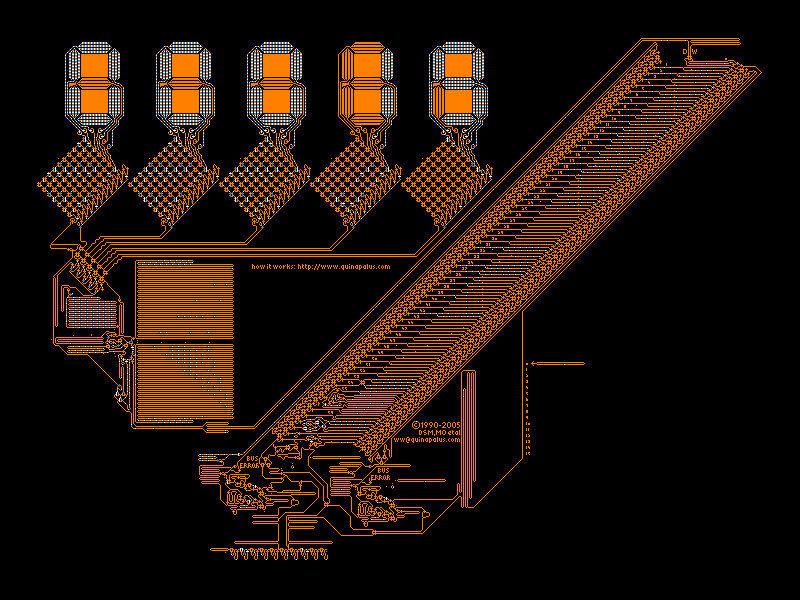
\includegraphics[width=0.8\textwidth]{../img/w12-lab/wireworld_computer.png}
    \end{center}
    \caption{En enkel dator implementerad i Wireworld.\protect\footnotemark}
    \label{fig:threads:life:wireworld-computer}
\end{figure}
\footnotetext{Källa: \url{http://www.quinapalus.com/wi-index.html}}


\subsection{Extra läsning}

\subsubsection{Intressanta mönster i Life}

\begin{itemize}[noitemsep,topsep=0pt]
    \item \url{https://en.wikipedia.org/wiki/Spacefiller}
    \item \url{https://en.wikipedia.org/wiki/Spaceship_(cellular_automaton)}
\end{itemize}

\subsubsection{Intressanta automater}

\begin{itemize}[noitemsep,topsep=0pt]
	\item \url{https://en.wikipedia.org/wiki/Codd's_cellular_automaton}
	\item \url{https://en.wikipedia.org/wiki/Von_Neumann_universal_constructor}
\end{itemize}

\subsubsection{Intressanta resurser}

\begin{itemize}[noitemsep,topsep=0pt]
    \item Eric Weisstein's Treasure Trove of the Life Cellular Automaton: \url{http://www.ericweisstein.com/encyclopedias/life/topics/}
\end{itemize}



% Kanske för nästa år
%\Task{Alternativ vy: Kör programmet i webbläsaren med Scala.js}


% Detta kan kräva speciell IDE (android-studio) och eventuellt en Android-emulator som inte kan köras på skolans datorer.
%\Task{Alternativ vy: Kör programmet på Android}


% Detta kommer antagligen inte ske då det lägger till signifikant komplexitet
% En bättre extrauppgift är att representera brädet som ett quadtree då det leder en in på Hashlife
%\Task{Implementera brädet som en sparse-matris}

%I den tidigare lösningen har vi allokerat en hel matris där bara en del av brädet vanligtvis är levande, en sådan matris kallas för en sparse matris (en matris där majoriteten av värdena är 0).
%    \Subtask{???}


%\Task{Implementera den supersnabba Hashlife}
%    Detta är en utmaning som kräver en viss kunskap om algoritmer och hashning som läsare av denna labben inte ännu förväntas inneha.
%    Den verkligt intresserade läsaren kan dock se denna uppgift som ett långtids-läromål och återkomma till uppgiften senare i sin utbildning när
%    hen känner sig redo.
%
%    En utförlig beskrivning om hashlife och quadtrees finnes på Wikipedia:
%    \begin{enumerate}
%        \item https://en.wikipedia.org/wiki/Hashlife
%        \item https://en.wikipedia.org/wiki/Quadtree
%    \end{enumerate}
%
%    \Subtask{Implementera QuadtreeMatrix2D}
%        Hashlife använder sig inte av en matris-representation för brädet utan använder sig istället av en datastruktur som heter Quadtrees.
%        Dessa fungerar som vanliga träd fast varje nod kan antingen ha exakt 4 brancher eller vara ett löv. Varje branchning delar upp en kvadrat
%        i 4 mindre kvadrater och varje löv representerar värdet för en kvadrat.
%
%        Quadtrees möjliggör att man kan beräkna tomma områden på brädet på konstant tid då man vet att ett helt område kommer förbli opåverkat utan
%        att behöva titta igenom varje cell.
%
%        \begin{figure}[h]
%            \begin{center}
%                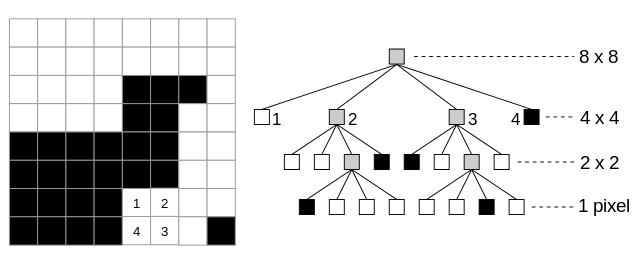
\includegraphics[width=0.7\textwidth]{../img/w12-lab/quadtree_bitmap.png}
%            \end{center}
%            \caption{Ett exempel på hur ett Quadtree använts för att representera en bitmap likt den som återfinns i Life}
%            % Källa: Wikipedia (https://commons.wikimedia.org/wiki/File:Quad_tree_bitmap.svg)
%        \end{figure}
%
%    \Subtask{Implementera hashlife}
%
%        Här kan vi inte handleda er, då det anses vara allt för långt utanför kursmålen. Men för den ambitiösa studenten refererar vi glatt till Wikipedia och önskar er lycka till!

%!TEX encoding = UTF-8 Unicode
%!TEX root = ../compendium.tex

\Assignment{bank}

\subsection{Fokus}
\begin{itemize}[nosep,label={$\square$},leftmargin=*]
\item Kunna implementera ett helt program efter given specifikation
\item Kunna sätta samman olika delar från olika moduler
\item Förstå hur Java-klasser kan användas i Scala
\item Förstå och bedöma när immutable/mutable såväl som var/val bör användas i större sammanhang
\item Kunna använda sig av kompanjons-objekt
\item Kunna läsa och skriva till fil
\item Kunna söka i olika datastrukturer på olika sätt
\end{itemize}

\subsection{Bakgrund}

I detta projekt ska du skriva ett program som håller reda på bankkonton och kunder i en bank. Programmet ska även hålla reda på bankens nuvarande tillstånd, såväl som föregående.
Tillstånden ska vid varje tillståndsförändring skrivas till fil så att ifall banken skulle krascha finns alla händelser som genomförts sparade, och banken kan således återställas.

Programmet ska vara helt textbaserat, man ska alltså interagera med programmet via konsollen där en meny skrivs ut och input görs via tangentbordet.

Du ska skriva hela programmet själv, med andra ord ges ingen färdig kod. Programmet ska dock följa de specifikationer som ges i uppgiften, såväl som de objektorienterade principer du lärt dig i kursen.

\subsection{Krav}

Kraven för bankapplikationen återfinns här nedan. För att bli godkänd på denna uppgift måste samtliga krav uppfyllas:

\begin{itemize}
\item Programmet ska ha följande menyval:

\begin{itemize}
\item 1. Hitta konton för en viss kontoinnehavare med angivet ID.
\item 2. Söka efter kunder på (del av) namn.
\item 3. Sätta in pengar på ett konto.
\item 4. Ta ut pengar på ett konto.
\item 5. Överföra pengar mellan två olika konton.
\item 6. Skapa ett nytt konto.
\item 7. Ta bort ett befintligt konto.
\item 8. Skriv ut bankens alla konton, sorterade i bokstavsordning efter innehavare.
\item 9. Återställa banken till ett tidigare tillstånd för ett givet datum. För enkelhetens skull får alla händelser genomförda efter det datum banken återställts till permanent kasseras. 
\item 10. Avsluta.
\end{itemize}

\item Programmet ska skapa ett nytt tillstånd med tidsstämpel och spara gamla tillstånd varje gång då:
\begin{itemize}
\item Pengar sätts in på ett konto
\item Pengar tas ut från ett konto.
\item Pengar överförs mellan två konton.
\item Ett konto skapas.
\item Ett konto tas bort.
\end{itemize}
\item Då bankens tillstånd förändras ska detta skrivas till fil.
\item Då banken startas upp ska händelsehistoriken läsas in så att banken laddar senaste sparade tillståndet.
\item Inga utskrifter eller inläsningar får göras i klasserna \code{Customer}, \code{BankAccount}, \code{Bank}, \code{State} eller \code{BankEvent}. Allt som berör användargränssnittet ska ske i \code{BankApplication}. Det är tillåtet att använda valfritt antal hjälpmetoder och hjälpklasser i \code{BankApplication}.
\item Alla metoder och attribut ska ha lämpliga åtkomsträttigheter.
\item Valen av val/var och immutable/mutable måste vara lämpliga.
\item Din indata måste ge samma resultat som i exemplen i bilagan.
\item Rimlig felhantering ska finnas, det är alltså önskvärt att programmet inte kraschar då man matar in felaktig input, utan istället säger till användaren att input är ogiltlig.
\item Programdesignen ska följa de specifikationer som är angivna nedan.
\item Det räcker med att banken ska kunna hantera heltal, men dessa ska ske med klassen \code{BigInt}.
\item Kontonummer ska genereras i klassen \code{BankAccount}, dessa ska vara unika för varje konto. Vid en tillståndförändringar ska dessa återställas, detta betyder att om en återställning tar bort ett konto så ska detta kontonummer återigen bli tillgängligt.
\end{itemize}

\subsection{Design}
Nedan följer specifikationerna för de olika klasserna bankapplikationen måste innehålla:

\begin{ScalaSpec}{Customer}
/**
 * Describes a customer of a bank with provided name and id.
 */
class Customer(val name: String, val id: Int) = {
	override def toString(): String = ???
}

\end{ScalaSpec}


\begin{ScalaSpec}{BankAccount}

/**
 * Creates a new bank account for the customer provided.
 * The account is given a unique account number and initially
 * has a balance of 0 kr.
 */
class BankAccount(val holder: Customer) = {

  /**
   * Deposits the provided amount in this account.
   */
  def deposit(amount: Int): Unit = ???

  /**
   * Returns the balance of this account.
   */
  def getBalance: Int = ???

  /**
   * Withdraws the provided amount from this account,
   * if there is enough money in the account. Returns true
   * if the transaction was successful, otherwise false. 
   */
  def withdraw(amount: Int): Boolean = ???

}
\end{ScalaSpec}


\begin{ScalaSpec}{BankEvent}
/**
 * Abstract class describing an event happening in the bank.
 */
abstract class BankEvent {   
  /**
   * Output format for the event.
   */
  def write: String
}

\end{ScalaSpec}


\begin{ScalaSpec}{Bank}

/**
 * Creates a new bank with no accounts and no state. 
 */
class Bank() = {

  /**
   * Adds a new account in the bank.
   * The account number generated for the account is returned.
   */
  def addAccount(name: String, id: Int): Int = ???

 /**
   * Removes the bank account with provided account number.
   * Returns true if successful, otherwise false is returned.
   */
  def removeAccount(accountNbr: Int): Boolean = ???

 /**
   * Returns a list of every bank account in the bank.
   * The returned list is sorted in alphabetical order based
   * on customer name.
   */
  def getAllAccounts(): ArrayBuffer[BankAccount] = ???

  /**
   * Returns the account holding the provided account number.
   * If no such account exists, null is returned.
   */
  def findByNumber(accountNbr: Int): BankAccount = ???

  /**
   * Returns a list of every account belonging to
   * the customer with the provided id.
   */
  def findAccountsForHolder(id: Int): ArrayBuffer[BankAccount] = ???

  /**
   * Returns a list of all customers whose names match
   * the provided name pattern.
   */
  def findByName(namePattern: String): ArrayBuffer[Customer] = ???

 /**
   * Executes an event in the bank.
   * Returns a string describing whether the
   * event was successful or failed.
   */
  def doEvent(event: BankEvent): String = ???

  /**
   * Resets the bank to the state with time-stamp corresponding to the
   * provided date. If the date provided doesn't correspond exactly to
   * any time-stamp then the nearest time-stamp with a date previous
   * to the provided date is used instead.
   * Returns a string describing whether the event was 
   * successful or failed.
   */
  def returnToState(returnDate: Date): String = ???

}
\end{ScalaSpec}


\begin{ScalaSpec}{State}

/**
 * Describes a bank state.
 * The queue log consists of a lists of all executed
 * BankEvents paired with the date each event was executed.
 */
class State(val log: Queue[(BankEvent, Date)]) 

\end{ScalaSpec}


För att använda tidsstämplar ska klassen \code{Date} som finns bifogat i kursens workspace användas. Detta är en enkel wrapper av \code{Java.time}.


\subsection{Tips} 

\begin{itemize}
\item För att representera tillstånden är det viktigt att alla händelser som förändrar tillståndet representeras av ett \code{BankEvent}.

\item För att skriva till fil på ett enkelt sätt kan man t.ex. använda sig av statiska metoder i klassen \code{Files} som finns tillgänglig i \code{java.nio.file}. För att undvika portabilitetsproblem kan man då använda sig av ett bestämt \code{Charset}, t.ex. \code{UTF_8}, som finns tillgänglig i \newline\code{java.nio.charset.StandardCharsets.UTF_8}.

\item För att läsa ifrån en fil kan man t.ex. använda sig av \code{Source} som finns tillgänglig i \code{scala.io.Source}. 

\item Var noggrann med att testerna klarar alla tänkbara fall, och tänk på att fler fall än dem som givits i exempel kan förekomma vid rättning.
\end{itemize}

\subsection{Obligatoriska uppgifter}

\Task Implementera klassen \code{Customer}.

\Task Implementera klassen \code{BankAccount}.

\Task Implementera den \code{BankEvent}-klass som skapar ett nytt konto.

\Task Skapa en ny klass \code{BankApplication}.

\Subtask Objektet \code{BankApplication} ska innehålla \code{main}-metoden. Det kan vara bra att innan man fortsätter se till att denna klass skriver ut menyn korrekt och kan ta input från tangentbordet som motsvarar de menyval som finns.

\Task Implementera klassen \code{Bank}.

\Subtask Implementera menyval 6 och 8. Testa noga.

\Subtask Implementera tillståndsfunktionaliteten. Varje nytt \code{BankEvent} ska ge upphov till ett nytt tillstånd och gamla tillstånd ska sparas som historik till det nya tillståndet.

\Subtask Implementera alla andra menyval, förutom menyval 9. Implementera även de klasser som förlänger \code{BankEvent} utefter att de behövs för nya menyval.
Testa de nya menyvalen noga efterhand som du implementerar dem, i synnerhet så att tillståndsförändringarna fungerar korrekt. Gör de utökningar du anser behövs. 

\Task Implementera menyval 9. När man försöker återställa banken till ett datum ska den senaste \code{BankEvent} genomförd före detta datum hämtas, med andra ord ska alla \code{BankEvent} med tidsstämpel efter återställningsdatumet kasseras permanent. Testa noga. Det är viktigt att denna funktionalitet fungerar bra innan man går vidare.

\Task Implementera säkerhetskopiering av tillstånden.

\Subtask Implementera utskriften till fil då ett nytt tillstånd skapas, utskriften ska ske omedelbart. Banken ska ej behöva avslutas för att utskriften ska hamna på fil, om så vore fallet kan information fortfarande gå förlorad om banken kraschar.

I repositoriet för denna projekt uppgift finns en sparfil bifogad, för bekvämlighet finns ett utdrag av denna fil  infogad nedanför. Inläsning och utskrift ska ske med dess format:\\~\\
2016 3 7 10 6 N 850127 Fredrik\newline
2016 3 7 10 28 D 1000 16500\newline
2016 3 9 10 52 W 1000 3900\newline
2016 3 9 11 8 N 900318 Casper\newline
2016 3 9 16 28 D 1001 6500\newline
2016 4 1 10 11 W 1001 1900\newline
2016 4 1 11 19 W 1001 2000\newline
2016 4 2 16 33 N 651002 Björn\newline
2016 4 2 16 46 D 1002 25000\newline
2016 4 3 10 11 T 1002 1000 4000\\~\\
Formen är alltså:\\~\\
\textbf{År  Månad  Dag  Timme  Minut  BankEventTag  Parametrar}
\\~\\
De olika klasserna av \code{BankEvent} representeras med följande bokstav:

\begin{itemize}
\item D - \code{Deposit}
\item W - \code{Withdraw}
\item T - \code{Transfer}
\item N - \code{NewAccount}
\item E - \code{DeleteAccount}
\end{itemize}

\Subtask Implementera inläsningen från fil då banken startas.


\subsection{Frivilliga extrauppgifter}

Gör först klart projektets obligatoriska delar. Därefter kan du, om du vill, utöka ditt
program enligt följande.

\Task Skriv en eller flera av klasserna \code{Customer}, \code{BankAccount} och \code{State} i Java istället och använd dig av dessa i din Scala-kod.

\Task	Implementera ett nytt menyalternativ som skriver ut all kontohistorik för en given person. I historiken ska finnas typ av händelse med tillhörande parametrar, dåvarande saldo vid händelsen, såväl som datumet för händelsen.

\subsection{Exempel på körning av programmet}

Nedan visas möjliga exempel på körning av programmet. Data som matas in av användaren är markerad i fetstil.
Ditt program måste inte se identiskt ut, men den övergripande strukturen såväl som resultat av körningen ska vara densamma.
När det första exemplet börjar förutsätts det att banken inte har några konton.

Listan över val, som är markerad i kursiv stil i det första exemplet, är inte utskriven i senare exempel för att spara plats på pappret. Ditt program ska alltid skriva ut listan över val före användaren ska mata in ett val.
\begin{multicols}{2}
\noindent
- - - - - - - - - - - - - - - - - - - - - - - - - - -\\*
\textit{
1.   Hitta ett konto för en given kund\\*
2.   Sök efter kunder på (del av) namn\\*
3.   Sätt in pengar\\*
4.   Ta ut pengar\\*
5.   Överför pengar mellan konton\\*
6.   Skapa nytt konto\\*
7.   Radera existerande konto\\*
8.   Skriv ut alla konton i banken\\*
9.   Återställ banken till ett tidigare datum\\*
10.  Avsluta\\*
}
Val: \textbf{6}\\*
Namn: \textbf{Adam Asson}\\*
Id: \textbf{6707071234}\\*
Nytt konto skapat med kontonummer: 1000\\*
10:03:0 CET 14 / 5 - 2016\\
- - - - - - - - - - - - - - - - - - - - - - - - - - -\\*
Val: \textbf{1}\\*
Id: \textbf{6707071234}\\*
Konto 1000 (Adam Asson, id 6707071234) 0 kr\\*
10:04:0 CET 14 / 5 - 2016\\
- - - - - - - - - - - - - - - - - - - - - - - - - - -\\*
Val: \textbf{6}\\*
Namn: \textbf{Berit Besson}\\*
Id: \textbf{8505255678}\\*
Nytt konto skapat med kontonummer: 1001\\*
10:12:0 CET 14 / 5 - 2016\\
- - - - - - - - - - - - - - - - - - - - - - - - - - -\\*
Val: \textbf{8}\\*
Konto 1000 (Adam Asson, id 6707071234) 0 kr\\*
Konto 1001 (Berit Besson, id 8505255678) 0 kr\\*
10:13:0 CET 14 / 5 - 2016\\
- - - - - - - - - - - - - - - - - - - - - - - - - - -\\*
Val: \textbf{2}\\*
Namn: \textbf{adam}\\*
Adam Asson, id 6707071234\\*
10:15:0 CET 14 / 5 - 2016\\
- - - - - - - - - - - - - - - - - - - - - - - - - - -\\*
Val: \textbf{6}\\*
Namn: \textbf{Berit Besson}\\*
Id: \textbf{8505255678}\\*
Nytt konto skapat med kontonummer: 1002\\*
13:56:0 CET 14 / 5 - 2016\\
- - - - - - - - - - - - - - - - - - - - - - - - - - -\\*
Val: \textbf{2}\\*
Namn: \textbf{erit}\\*
Berit Besson, id 8505255678\\*
14:01:0 CET 14 / 5 - 2016\\
- - - - - - - - - - - - - - - - - - - - - - - - - - -\\*
Val: \textbf{3}\\*
Kontonummer: \textbf{1000}\\*
Summa: \textbf{5000}\\*
Transaktionen lyckades.\\*
14:36:0 CET 14 / 5 - 2016\\
- - - - - - - - - - - - - - - - - - - - - - - - - - -\\*
Val: \textbf{5}\\*
Kontonummer att överföra ifrån: \textbf{1000}\\*
Kontonummer att överföra till: \textbf{1001}\\*
Summa: \textbf{1000}\\*
Transaktionen lyckades.\\*
14:37:0 CET 14 / 5 - 2016\\
- - - - - - - - - - - - - - - - - - - - - - - - - - -\\*
Val: \textbf{8}\\*
Konto 1000 (Adam Asson, id 6707071234) 4000 kr\\*
Konto 1001 (Berit Besson, id 8505255678) 1000 kr\\*
Konto 1002 (Berit Besson, id 8505255678) 0 kr\\*
14:52:0 CET 14 / 5 - 2016\\
- - - - - - - - - - - - - - - - - - - - - - - - - - -\\*
Val: \textbf{7}\\*
Ange konto att radera: \textbf{1002}\\*
Transaktionen lyckades.\\*
14:01:0 CET 14 / 5 - 2016\\
- - - - - - - - - - - - - - - - - - - - - - - - - - -\\*
Val: \textbf{8}\\*
Konto 1000 (Adam Asson, id 6707071234) 4000 kr\\*
Konto 1001 (Berit Besson, id 8505255678) 1000 kr\\*
14:01:0 CET 14 / 5 - 2016\\
- - - - - - - - - - - - - - - - - - - - - - - - - - -\\*
Val: \textbf{9}\\*
Vilket datum vill du återställa banken till?\\*
År: \textbf{2016}\\*
Månad: \textbf{5}\\*
Datum (dag): \textbf{9}\\*
Timme: \textbf{18}\\*
Minut: \textbf{10}\\*
Banken återställd.\\*
15:00:0 CET 14 / 5 - 2016\\
- - - - - - - - - - - - - - - - - - - - - - - - - - -\\*
Val: \textbf{8}\\*
Konto 1002 (Björn, id 651002) 25900 kr\\*
Konto 1001 (Casper, id 900318) 4600 kr\\*
Konto 1003 (Eva, id 950908) 6300 kr\\*
Konto 1000 (Fredrik, id 850127) 11800 kr\\*
Konto 1004 (Kajsa, id 810722) 17000 kr\\*
15:01:0 CET 14 / 5 - 2016\\
- - - - - - - - - - - - - - - - - - - - - - - - - - -\\*
Val: \textbf{3}\\*
Kontonummer: \textbf{1005}\\*
Summa: \textbf{5000}\\*
Transaktionen misslyckades. Inget sådant konto hittades.\\*
15:06:0 CET 14 / 5 - 2016\\
\end{multicols}

%!TEX encoding = UTF-8 Unicode
%!TEX root = ../compendium.tex

\Assignment{tictactoe}

\begin{Goals}
	\item Implementera ett helt program efter specifikation.
	\item Få en inblick i hur rekursion kan användas, utöver svans-rekursion.
	\item Bli introducerad till spelteori och hur man kan uttrycka optimal strategi för spelet tictactoe.
	\item Träna på att använda abstrakta klasser.
	\item Kunna byta mellan representationer av en spelplan.
\end{Goals}

\subsection{Bakgrund}
I detta projektet ska du implementera din egen version av spelet tic-tac-toe (eller som vi på svenska kallar det, tre i rad)! Du kommer börja med att implementera en version där du kan spela mot en kursare och sen gå vidare till att implementera en datorspelare som lägger sin pjäs slumpmässigt och till slut en som inte kan förlora!

\subsection{Regler}
Om du känner dig säker på hur reglerna i tic-tac-toe funkar kan du skippa detta.\footnote{\href{https://en.wikipedia.org/wiki/Tic-tac-toe}{en.wikipedia.org/wiki/Tic-tac-toe}}
\begin{itemize}
	\item Spelplanen består av ett rutnät av storlek 3x3.
	\item Det finns två spelare: \texttt{x} och \texttt{o}.
	\item Spelarna placerar ut en pjäs var i växlande ordning där \texttt{x} börjar.
	\item Om en spelare har fått antingen en rad, diagonal eller kolumn ifylld av sin spelpjäs vinner den spelaren. Om hela spelplanen blir fylld utan att någon vinner slutar spelet oavgjort.
\end{itemize}
\textit{Notera att pjäserna INTE får flyttas när de väl ligger på spelplanen.}

\subsection{Teori}

Representationen är vald till en endimensionell array av typen \code{Int} av storlek 9 där element $[0,2]$\footnote{Med beteckningen $[x,y]$ menas alla heltal från och med $x$ till och med $y$, dvs: $x$, $x+1$, $x+2$, \ldots , $y-1$, $y$. Kortfattat så är $[0,2]$ = \code{\{0,1,2\}}.} representerar den första raden, $[3,5]$ den andra och $[6,8]$ den tredje. Anledningen till detta är att vi vill ha en representation så att spelaren kan svara vilket drag den vill göra med ett heltal.
Varje element i arrayen ska kunna representera en tom plats, en plats allokerad av \texttt{x} och en plats allokerad av \texttt{o}. Detta innebär att en array av typen \code{Boolean} inte räcker till. Istället väljs den (kanske lite minnesöverflödiga) typen \code{Int}. Vi har valt representationen där 0 representerar tom plats, 1 representerar \texttt{x} och -1 representerar \texttt{o}. Denna representation är smidig dels för vår framtida \code{OptimalPlayer} och dels för att avgöra om spelare \texttt{x} eller \texttt{o} har vunnit. Man kan exempelvis summera en rad och kolla om radens summa är 3 (då har \texttt{x} vunnit) eller -3 (då har \texttt{o} vunnit).

\subsection{Design}
Den här uppgiften kommer innehålla lite färre klasser och mindre objekt\-orienterade utmaningar, men istället lite klurigare algoritmiska utmaningar. Vi skall dessutom använda rekursion till vår fördel, vilket för den ovane brukar vara krångligt, därför hamnar huvudfokus här. Programmet har följande klasstruktur:

\code{Game}. I sin mainmetod frågar den användaren hur spelen skall gå till och med vilka spelare.
När detta är specificerat anropas den rekursiva metoden \code{play}.
\code{play} spelar ett spel mellan två spelare tills någon vinner eller det blir oavgjort.
Kodskelettet för \code{Game} ser ut på följande vis:
\begin{ScalaSpec}{Game}
/** 
 * Asks the user what kind of players should play against each other.
 * Creates the players that the user chooses via System.in 
 * Asks the user if the board should be drawn.
 * If the board should not be drawn, ask the user for n,
 * the amount of games that should be played between the two players.
 * Else n = 1.
 * Call play n times with the two players, an empty board, depth = 0,
 * and drawing true/false dependent on if the board should be printed or not. 
 * Save the resuts from play. 
 * Present the results after n games have been played. 
 */
def main(args: Array[String]): Unit = ???

/**
 * p1 and p2 are the players that should play the game.
 * depth models amount of moves done by both players.
 * drawing is true if draw should be called before each move.
 *(1) If drawing: call draw(game)
 *(2) If game is won by any of the players, or depth == 9, 
 * return 1 if p1 wins, -1 if p2 wins and 0 if there is a draw.
 *(3) Else: Asks player 1 for its move if depth%2 == 0, else ask player 2.
 *(4) Update game according to the move p1 or p2 does.
 *(5) Return play(p1,p2,game,depth+1,drawing) (if someone wins with
 * the current move, it will be detected by (2) in this call of play)
 */
def play(p1: Player, p2: Player, game: Array[Int], 
         depth: Int, drawing: Boolean): Int = ???

/**
 * Given an Array[Int] game of size 9, 
 * print the 3x3 board that the array represents. 
 * [0,2] is the 1st, [3,5] is the 2nd and [6,8] is the 3rd row.
 * -1 should be represented by 'o', 0 with '.' and 1 with 'x'.
 * In particular, [0,1,-1,0,0,1,0,1,-1] should print:
 * .xo
 * ..x
 * .xo
 */

def draw(game:Array[Int]): Unit = ???
\end{ScalaSpec}

\code{Player}. Denna abstrakta klass kommer innehålla gemensam logik för players. För att inte göra våra players beroende av \code{Game }har vi valt att lägga en metod \code{gameWon} i \code{Player}. Valet av placering av denna metod kan definitivt diskuteras. Man skulle kunna tänka sig att denna metod borde ligga i ett util-objekt eller liknande, men för tillfället är det bara denna metod som man skulle vilja ha i ett sådant objekt vilket gör det klumpigt. Anledningen till att den istället hamnat hos \code{Player} är att både \code{OptimalPlayer} och \code{FastOptimalPlayer} ärver från \code{Player} och kommer vilja ha tillgång till denna metod.

\code{Player}s viktiga funktion är dess \code{move}-metod. Det är denna metod som kommer skilja sig för olika players. I den första uppgiftern skall ett tal (draget) läsas in i \code{HumanPlayer}s \code{move}-metod, och i nästkommande uppgift skall ett slumpmässigt drag väljas i \code{RandomPlayer}s \code{move}-metod.
Kodskelettet för \code{Player} ser ut på följande sätt:
\begin{ScalaSpec}{Player}
abstract class Player(name: String) {
	
	/**
	 * Abstract method. Should not be implemented here, 
	 * but required by subtypes of Player.
	 * Returns an int p in the interval [0,8] where game(p) == 0,
	 * the index of the move this player does. 
	 */
	def move(game: Array[Int], depth: Int): Int;
	
	/**
	 * Returns true if there exists a row, column or diagonal,
	 * where all the elements are equal to who.
	 */
	def gameWon(game: Array[Int], who: Int): Boolean = ???
	
	// returns a String with information about the player.
	override def toString(): String = ???
}
\end{ScalaSpec}

 
\subsection{Obligatoriska uppgifter}

\Task Implementera ett fungerande spel genom att utöka kodskeletten i klasserna \code{Player}, \code{HumanPlayer} och \code{Game}.

\Subtask Implementera metoden \code{gameWon} i klassen \code{Player} som testar huruvida spelaren \code{who} vunnit spelet.

\Subtask Implementera \code{HumanPlayer}s \code{toString}-metod.

\Subtask Implementera \code{HumanPlayer}s \code{move}-metod.

\Subtask Implementera en version av \code{Game}. Börja med att alltid spela ett spel och alltid rita spelplanen. \code{main}, \code{draw} och \code{play} behöver implementeras. All funktionalitet i \code{main} behöver inte finnas ännu.\footnote{Notera att man behöver invertera spelplanen om den ska skickas till spelare två (alternativt låta spelaren hålla reda på om den är \texttt{x} eller \texttt{o}). Förslagsvis löses detta med en extra metod \code{invertGame} som skapar en ny array med omvända tecken till orginalarrayen.}

\Task \code{RandomPlayer}

\Subtask Skapa en ny klass som ärver från \code{Player} (kopiera \code{HumanPlayer}, och byt namn till \code{RandomPlayer}) där \code{move} istället för att läsa från \code{System.in} väljer ett slumpmässigt giltigt drag.

\Subtask Ändra \code{Game} så att användaren tillåts stänga av ritfunktionen och i så fall tillåts välja antalet spel.

\Subtask Vad är sannolikheterna för att \texttt{x} vinner, \texttt{o} vinner och att det blir oavgjort om två \code{RandomPlayer}s spelar mot varandra?

Hamnar man i närheten av dessa resultat tror vi på er \code{RandomPlayer}.
\begin{itemize}
	\item P(\texttt{x} vinner) = 0.586
	\item P(\texttt{o} vinner) = 0.288
	\item P(lika) = 0.126
\end{itemize}

\Subtask Varför är det större sannolikhet för \texttt{x} att vinna än \texttt{o}?

\Task \code{OptimalPlayer}

Betrakta den givna funktionen \code{eval}.
\begin{Code}
/**
 * Return 1 if there is a guaranteed strategy for who to win.
 * Return 0 if there is a guaranteed strategy for who to draw.
 * Return -1 if opponent can force a win no matter what who does.
 * This is done by min,max evaluation.
 * Find the move that gives the opponent the worst possible
 * position (min) and return -min, this is our max.
 * depth is the amount of placed cells (!=0) in game.
 * who is 1 if it's this player's turn to make a move,
 * -1 if it's the opponent's turn to make a move. 
 * From move, eval should be called with who = -1.
 */
def eval(game: Array[Int], depth: Int, who: Int): Int = {
	if (gameWon(game, -who)) return -1
	if (depth == 9) return 0
	var min = 1
	for (i <- 0 until 9) {
		if (game(i) == 0) {
			game(i) = who
			val score = eval(game, depth + 1, -who)
			if (score < min) {
				min = score
			}
			game(i) = 0
		}
	}
	-min
}
\end{Code}

\code{eval} avgör om du är i en vinnande, förlorande eller oavgjord situation, givet att båda spelare spelar optimalt. Det som nog är svårast att förstå är varför vi returnerar \code{-min} på slutet. \code{min} sparar det sämsta värdet som vår motståndare kan få givet våra möjliga drag. Vi observerar att vi är i precis omvänd situation jämfört med vår motståndare. Om vår motståndare definitivt vinner förlorar vi definitivt, om det blir oavgjort för vår motståndare blir det också oavgjort för oss, och om vår motståndare definitivt förlorar, då vinner vi. Vi representerade ju vinst med 1, oavgjort med 0 och förlust med -1. Det är alltså härifrån minustecknet kommer ifrån. Vill man läsa mer om detta kan man kolla in Wikipedias artikel om minmax-evaluering.\footnote{\url{https://en.wikipedia.org/wiki/Minimax}} Vi tar helt enkelt det draget som är sämst för vår motståndare.

\Subtask Implementera \code{move-metoden} i \code{OptimalPlaye}r genom att anropa \code{eval}.

\Subtask Låt två \code{OptimalPlayer}s spela mot varandra. Det skall alltid bli oavgjort.

\Subtask Testa att spela mot din \code{OptimalPlayer} med en \code{HumanPlayer}. Kan du spela lika? Kan du vinna?

\Subtask Vad händer om du sätter en \code{RandomPlayer} mot \code{OptimalPlayer}? Blir det någonsin oavgjort? Hur ofta? Bilr det någon skillnad om man byter vem som får spela först?

\Task Utöka säkerheten och isoleringen av ditt program

I nuläget finns det förmodligen ett problem med din nuvarande implementation, och det är att du skickar iväg en förändringsbar datastruktur till en \code{Player} som utifrån den förändringsbara datan skall göra ett drag. Tänk om en elak programmerare bestämmer sig för att ändra på spelplanen i sin egna players \code{move}-metod. Då skulle man i princip kunna fuska. För att lösa detta kan man från \code{Game} istället för att ge ifrån sig den egna representationen av spelplanen göra en kopia och ge kopian till \code{Player}n.

\Task Snabbare \code{OptimalPlayer}

Om du låter en \code{OptimalPlayer} spela mot en \code{RandomPlayer} 1000 gånger lär det ta ganska lång tid. Det behöver det inte göra. När \code{OptimalPlayer} bestämmer vilket drag den skall göra första gången går den ju igenom alla andra möjliga drag man kan komma till. Det visar sig att det inte finns så många unika spelbräden. Färre än $3^9 < 20000$. 

Skapar vi istället en \code{Map} som innehåller ett värde för varje spelbräde kommer vi kunna spela mycket snabbare när vår \code{Map} väl är genererad. Skillnaden i snabbhet för vårt program blir alltså att vi behöver göra ett uppslag i en \code{Map}, jämfört med ungefär $9! > 300000$ funktionsanrop för ett drag på ett tomt spelbräde. 

Det räcker med att modifiera evalueringsmetoden något för att bygga \code{Map}en. Anropa sedan denna med ett tomt bräde, så har vi vår \code{Map} och vår optimala spelare är nu supersnabb!

Man får dock vara lite klurig. En \code{Array[Int]} går inte att använda som nyckel i en \code{Map} i Java, då den inte har en implementerad \code{hashCode}-metod. I Scala är det tillåtet, men mappningen kommer att vara på referenslikhet och inte innehållslikhet, vilket vi i det här fallet inte vill. Enklast, som fungerar säkert i både Java och Scala, är att göra om vår array till en sträng genom att lägga värdena i arrayen efter varandra i strängen. Vi kan göra en privat metod \code{hash(Array[Int]): String} som konkatenerar värdena i arrayen. \code{hash([0,0,0,1,1,0,-1,-1,0])} skall alltså returnera \code{"000110-1-10"}.

\Subtask Skapa en ny subklass till \code{Player}: \code{FastOptimalPlayer}.

\Subtask Skapa och implementera en privat metod \code{hash(Array[Int]): String}.

\Subtask Implementera en konstruktor som skapar och genererar en \code{Map}.

En \code{Map} kan initieras på följande vis:
\begin{Code}
val boardCache = scala.collection.mutable.Map.empty[String, Int]
\end{Code}

För att sedan generera vår \code{Map} krävs en metod som motsvarar \code{eval}-metoden i \code{OptimalPlayer}. Denna kan tas rakt av, men med två små modifikationer:
\begin{itemize}
\item Vid start: Om det redan finns ett key-value-par i \code{Map}en: returnera det parets värde.
\item Vid slut: Innan du returnerar måste ett key-value-par läggas in i den \code{Map} som vi genererar.
\end{itemize}
Denna metod bör sedan anropas i slutet av konstruktorn med ett tomt \code{board}.


\Subtask Låt \code{move}-metoden göra ett \code{Map}-uppslag med hjälp av \code{hash}-metoden och din \code{Map}.

\Subtask Testa att låta en \code{FastOptimalPlayer} spela mot en \code{RandomPlayer}. Du märker nog att skapandet av en \code{FastOptimalPlayer} kommer ta lite tid, runt en halv sekund. Sedan skall det dock gå jättesnabbt när spelarna spelar. 100000 spel skall gå utan problem på någon sekund, vilket borde gå på tiotals minuter för den gamla \code{OptimalPlayer}.

%!TEX encoding = UTF-8 Unicode
%!TEX root = ../compendium.tex

\Assignment{imageprocessing}

\subsection{Bakgrund}

En digital bild består av ett rutnät (en matris) av pixlar. Varje pixel har en färg, och om man har många pixlar flyter de samman för ögat så att de tillsammans skapar en bild.

Det finns olika system för hur man färgsätter de olika pixlarna. T.ex. så används CMYK-systemet (cyan, magenta, gul, svart) vid blandning av färg som ska tryckas på papper eller annat material. På en dator däremot används vanligtvis RGB-systemet. RGB-systemet har tre grundfärger: röd, grön och blå. Mättnaden av varje grundfärg anges av ett heltal som vi i fortsättningen förutsätter ligger i intervallet [0, 255]. 0 anger ”ingen färg” och 255 anger ”maximal färg”. Man kan därmed representera 256 × 256 × 256 = 16 777 216 olika färgnyanser. Man kan också representera gråskalor; det gör man med färger som har samma värde på alla tre grundfärgerna: (0, 0, 0) är helt svart, (255, 255, 255) är helt vitt.


\subsection{Uppgiften}
Du ska skriva ett program där du implementerar olika filter som ska manipulera en given bild på ett flertal olika sätt. Filterklasserna ska ärva från en abstrakt \code{ImageFilter}-klass som är skriven i Java. \code{ImageFilter}-klassen hittar du i cslib.

Följande beskriver \code{ImageFilter}-klassen.

\begin{JavaSpec}{abstract class ImageFilter}
/**
 * Skapar ett filterobjekt med ett givet namn och antalet argument.
 */
protected ImageFilter(String name, int nbrOfArgs);

/**
 * Tar reda på filtrets namn.
 */
public String getName();

/**
 * Tar reda på antalet argument filtret behöver till apply-metoden.
 */
public int getNumberOfArguments();

/**
 * Filtrerar bilden i matrisen inPixels och returnerar resultatet i 
 * en ny matris. Utnyttjar eventuellt värdena i args.
 */
public abstract Color[][] apply(Color[][] inPixels, double[] args);


/**
 * Beräknar intensiteten hos alla pixlarna i pixels,
 * returnerar resultatet i en ny matris.
 */
protected short[][] computeIntensity(Color[][] pixels):

/**
 * Faltar punkten p[i][j] med faltningskärnan kernel.
 * 
 * @param p 		matris med talvärden
 * @param i 		radindex får den aktuella punkten
 * @param j 		kolonnindex får den aktuella punkten
 * @param kernel	faltningskärnan, en 3x3-matris
 * @param weight	summan av elementen i kernel
 * @return 		resultatet av faltningen
 */
protected short convolve(short[][] p, int i, int j, 
			short[][] kernel, int weight);
\end{JavaSpec}

Utöver filterklasserna ska du även skapa ett program där du kan välja ett variabelt antal filter och sedan applicera dessa på en bild. För att åstadkomma detta ska du implementera klasserna \code{FilterChooser}, som hanterar val av filter, och \code{FilterList} som representerar vilka filter som ska användas. Klasserna har följande specifikationer:

\begin{ScalaSpec}{FilterList}
class FilterList = ???

/** Adds a filter to the FilterList */
def addFilter(filter: ImageFilter): Unit = ???
  
/** Applies all the filters on the given Image and draws it in SimpleWindow */
def applyFilters(image: Image, sw: SimpleWindow): Unit = ???
\end{ScalaSpec}

\begin{ScalaSpec}{FilterChooser}
/** Creates a FilterChooser with all the available filters */
class FilterChooser(filters: Array[ImageFilter]) = ???
  
/** Shows which filters are available and lets the user choose filters
*   until an escape sequence has been given and returns a FilterList which
*   contain the chosen filters
*   Example: 
*   0. för Blått-filter
*   2. för Kontrast-filter
*   3. för Gauss-filter
*   4. för Sobel-filter
*   5. om du inte vill ha fler filter
*/
def chooseFilters(): FilterList = ???
\end{ScalaSpec}

Till din hjälp får du en \code{Image}-klass som representerar en bild samt ett \code{ImageUI} som hjälper dig att ladda in en JPEG bild.

\begin{ScalaSpec}{Image}
class Image(val image: BufferedImage);

/** Returns a matrix of Color-objects that represents an image */
def getColorMatrix: Array[Array[Color]];

/** Updates the image in accordance with the given Color-matrix */
def updateImage(pixels: Array[Array[Color]]): Unit;
\end{ScalaSpec}

\begin{ScalaSpec}{ImageUI}
object ImageUI;

/** Returns a chosen image from the images folder.
*   Prints:	
*  
*   Välj en av följande bilder genom att mata in en siffra
*
*   0. boy.jpg
*   1. car.jpg
*   2. duck.jpg
*   3. facade.jpg
*   4. jay.jpg
*   5. moon.jpg
*   6. obidos.jpg
*   7. sgrada.jpg
*   8. shuttle.jpg
*   Ditt val: 
*/
def getImage: BufferedImage;
\end{ScalaSpec}


\Task \textbf{Blåfilter.} Skriv en klass \code{BlueFilter} som skapar en blå version av bilden. Det vill säga skapa ett filter där varje pixel bara innehåller den blå komponenten. Testa filtret genom att skapa ett \code{ImageProcessing}-object som ska innehålla en \code{main}-metod (\code{ImageProcessing} ska användas och utökas i senare uppgifter). Använd \code{ImageUI} för att välja en bild på följande sätt:
\begin{Code}
val im = new Image(ImageUI.getImage)
\end{Code}
Använd \code{SimpleWindow} samt \code{image} attributet från \code{Image}-objektet för att visa bilden. 

\Task \textbf{Inverteringsfilter.} Skriv en klass \code{InvertFilter} som inverterar en bild dvs skapar en ''negativ'' kopia av bilden. Ljusa färger ska alltså bli mörka och mörka färger ska bli ljusa.
Fundera över vad som kan menas med en inverterad eller negativ kopia: de nya RGB-värdena är inte ett dividerat med de gamla värdena (då skulle de nya värdena kunna bli flyttal) och inte de gamla värdena med ombytt tecken (då skulle de nya värdena bli negativa).

\Task \textbf{Gråskalningsfilter.} Skriv en klass \code{GrayScaleFilter} som gör om bilden till en gråskalebild. Använd \code{ImageFilter}s \code{computeIntensity} metod för att bestämma vilken intensitet varje pixel ska ha. Om intensiteten i en pixel till exempel är 105 så ska ett nytt \code{Color}-objekt med värdena (105, 105, 105) skapas.

\Task \textbf{Krypteringsfilter.} Skriv en klass \code{XORCryptFilter} som krypterar bilden med xor-operatorn ˆ. Denna operator gör binär xor mellan bitarna i ett heltal. Exempelvis ger 8 ˆ 127 värdet 119. Om man gör xor igen med 127, alltså 119 ˆ 127, får man tillbaka värdet 8. Varje pixel krypteras genom att använda xor-operatorn med ursprungsvärdena för rött, grönt och blått tillsammans med ett slumpmässigt heltalsvärde som genereras av Scalas Random klass. Använd \code{paramValue} för att ge \code{Random}-objektet ett seed. På så sätt kan du återskapa bilden genom att applicera krypteringsfiltret igen, med samma \code{paramValue}, på den numera krypterade bilden.

\Task \textbf{Gaussfiltrer.} Gaussfiltrering är ett exempel på så kallad faltningsfiltrering. Filtreringen bygger på att man modifierar varje bildpunkt genom att titta på punkten och omgivande punkter. 

För detta utnyttjar man en så kallad faltningskärna K som är en liten kvadratisk heltalsmatris. Man placerar K över varje element i intensitetsmatrisen och multiplicerar varje element i K med motsvarande element i intensitetsmatrisen. Man summerar produkterna och dividerar summan med summan av elementen i K för att få det nya värdet på intensiteten i punkten. Divisionen med summan gör man för att de nya intensiteterna ska hamna i rätt intervall.

Exempel:

\begin{minipage}{5cm}
\begin{displaymath}
\mathit{intensity} = \left(
\begin{array}{ccccc}
5 & 4 & 2 & 8 & \ldots \\
4 & 3 & 4 & 9 & \ldots \\
9 & 8 & 7 & 7 & \ldots \\
8 & 6 & 6 & 5 & \ldots \\
\vdots & \vdots & \vdots & \vdots & \ddots
\end{array}
\right)
\end{displaymath}
\end{minipage}\hspace{2cm}
\begin{minipage}{5cm}
\begin{displaymath}
K = \left(
\begin{array}{ccc}
0 & 1 & 0 \\
1 & 4 & 1 \\
0 & 1 & 0
\end{array}
\right)
\end{displaymath}
\end{minipage}

Här är summan av elementen i $K$ $1+1+4+1+1 = 8$. För att räkna ut det nya värdet på intensiteten i punkten med index \code{(1)(1)} (det nuvarande värdet är 3) beräknar man:

\begin{displaymath}
\mathit{newintensity} = \frac{0 \cdot 5 + 1 \cdot 4 + 0 \cdot 2 + 1 \cdot 4 + 4 \cdot 3 + 1 \cdot 4 + 0 \cdot 9 + 1 \cdot 8 + 0 \cdot 7}{8} = \frac{32}{8} = 4
\end{displaymath}


Man fortsätter med att flytta K ett steg åt höger och beräknar på motsvarande sätt ett nytt värde för elementet med index \code{(1)(2)} (där det nuvarande värdet är 4 och det nya värdet blir 5). Därefter gör man på samma sätt för alla element utom för ”ramen” dvs elementen i matrisens ytterkanter.

Skriv en klass \code{GaussFilter}som implementerar denna algoritm. Varje färg ska behandlas separat. Gör på följande sätt:
\begin{enumerate}
	\item Bilda tre short-matriser och lagra pixlarnas red-, green- och blue-komponenter i matriserna.
	\item Utför faltningen av de tre komponenterna för varje element och lagra ett nytt \code{Color}-objekt i \code{outPixels} för varje punkt.
	\item Elementen i ramen behandlas inte, men i \code{outPixels} måste också dessa element få värden. Enklast är att flytta över dessa element oförändrade från \code{inPixels} till \code{outPixels}. Man kan också sätta dem till \code{Color.WHITE}, men då kommer den filtrerade bilden att se något mindre ut.
\end{enumerate}

Använd \code{ImageFilter}s \code{convolve}-metod för att utföra faltningen. Metoden behöver en faltningsmatris, \code{kernel}, som input och ska anropas med red-, green- och blue-matrisen. Faltningsmatrisen kan vara ett attribut i klassen och ska ha följande utseende:

\begin{displaymath}
\begin{pmatrix}
  0 & 1 & 0 \\
  1 & 4 & 1 \\
  0 & 1 & 0 \\
\end{pmatrix}
\end{displaymath}

Det kan vara intressant att prova med andra värden än 4 i mitten av faltningsmatrisen. Med värdet 0 får man en större utjämning eftersom man då inte alls tar hänsyn till den aktuella pixelns värde. Mata in detta värde i Parameter-rutan. 

Anmärkning: det kan ibland vara svårt att se någon skillnad mellan den filtrerade bilden och originalbilden. Om man vill ha en riktigt suddig bild så måste man använda en större matris som faltningskärna.


\Task  \textbf{Sobelfiltrer.} Sobelfiltrering är, precis som Gaussfiltrering, en typ av faltningsfiltrering. Med Sobelfiltrering får man dock motsatt effekt i jämförelse med Gaussfiltrering, dvs man förstärker konturer i en bild. I princip deriverar man bilden i x- och y-led och sammanställer resultatet.

\begin{figure}[H]
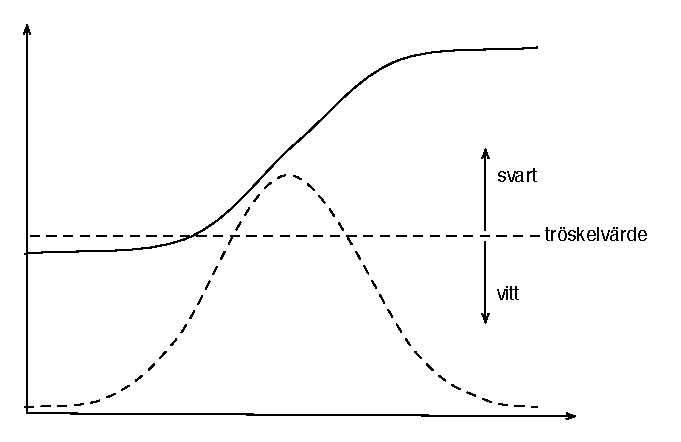
\includegraphics[width=0.9\textwidth]{../img/w13-assignment-imageprocessing/derivatabild2.pdf}
\caption { En funktion (heldragen linje) och dess derivata (streckad linje).}
\label{fig:imageprocessing:sobelfilter:derivatabild}
\end{figure}

I figur~\ref{fig:imageprocessing:sobelfilter:derivatabild} visas en funktion $f$ (heldragen linje) och funktionens derivata $f'$ (streckad linje). Vi ser att där funktionen gör ett ''hopp'' så får derivatan ett stort värde. Om funktionen representerar intensiteten hos pixlarna längs en linje i x-led eller y-led så motsvarar ''hoppen'' en kontur i bilden. Om man sedan bestämmer sig för att pixlar där derivatans värde överstiger ett visst tröskelvärde ska vara svarta och andra pixlar vita så får man en bild med bara konturer. 

Nu är ju intensiteten hos pixlarna inte en kontinuerlig funktion som man kan derivera enligt vanliga matematiska regler. Men man kan approximera derivatan, till exempel med följande formel:

\begin{displaymath}
f'(x) \approx \frac{f(x+h) - f(x-h)}{2h}
\end{displaymath}

(Om man här låter $h$ gå mot noll så får man definitionen av derivatan.) Uttryckt i Scala och matrisen \code{intensity} så får man:

\begin{Code}
val derivative = (intensity(i)(j+1) - intensity(i)(j-1)) / 2
\end{Code}

Allt detta kan man uttrycka med hjälp av faltning. 

\begin{enumerate} 
	\item Beräkna intensitetsmatrisen med metoden \code{computeIntensity}.
	\item Falta varje punkt i intensitetsmatrisen med två kärnor:
$$
X\_SOBEL =
\begin{pmatrix}
  -1 & 0 & 1 \\
  -2 & 0 & 2 \\
  -1 & 0 & 1 \\
\end{pmatrix}
Y\_SOBEL =
\begin{pmatrix}
  -1 & -2 & -1 \\
  0 & 0 & 0 \\
  1 & 2 & 1 \\
\end{pmatrix}
$$
	Använd metoden \code{convolve} med vikten 1. Koefficienterna i matrisen $X\_SOBEL$ uttrycker derivering i x-led, i $Y\_SOBEL$ faltning i y-led. För att förklara varför koefficienterna ibland är 1 och ibland 2 måste man studera den bakomliggande teorin noggrant, men det gör vi inte här.
	\item Om resultaten av faltningen i en punkt betecknas med \code{sx} och \code{sy} så får man en indikator på närvaron av en kontur med \code{math.abs(sx) + math.abs(sy)}. Absolutbelopp behöver man eftersom man har negativa koefficienter i faltningsmatriserna. 
	\item  Sätt pixeln till svart om indikatorn är större än tröskelvärdet, till vit annars. Tröskelvärdet bestäms av \code{paramValue}. 
\end{enumerate}

Skriv en klass \code{SobelFilter} som implementerar denna algoritm.

\begin{figure}[H]
\begin{center}
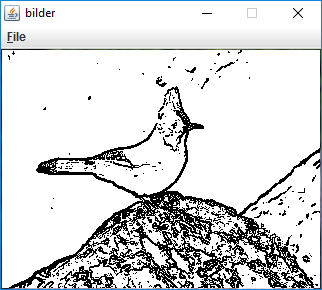
\includegraphics[width=0.6\textwidth]{../img/w13-assignment-imageprocessing/sobeljay.png}
\caption { Exempel på en bild där ett Sobelfilter applicerats med ett parametervärde på 150.}
\label{fig:imageprocessing:sobelfilter:sobel}
\end{center}
\end{figure}


\Task Implementera \code{FilterList} enligt specifikationerna ovan.

\Task Implementera \code{FilterChooser} enligt specifikationerna ovan.

\Task Knyt ihop allt i \code{ImageProcessing}-objektet som du skapade innan. Utskrifterna ska se ut på följande sätt:

{\setlength{\parindent}{0cm}

 Välj en av följande bilder genom att mata in en siffra\newline

0. boy.jpg\newline
1. car.jpg\newline
2. duck.jpg\newline
3. facade.jpg\newline
4. jay.jpg\newline
5. moon.jpg\newline
6. obidos.jpg\newline
7. sgrada.jpg\newline
8. shuttle.jpg\newline
Ditt val: \textbf{1}\newline
Bild car.jpg laddad\newline
0. för Vanligt-filter\newline
1. för Blått-filter\newline
2. för Krypterat-filter\newline
3. för Inverterat-filter\newline
4. för Grått-filter\newline
5. för Kontrast-filter\newline
6. för Gauss-filter\newline
7. för Sobel-filter\newline
8. om du inte vill använda fler filter\newline
Välj ett filter \textbf{1}\newline
Välj ett filter \textbf{8}\newline
Välja ny bild? (y/n) \textbf{n}\newline
}

Tänk på att användaren kan mata in otillåtna värden. Detta ska hanteras på lämpligt sätt.

\subsection{Frivilliga extrauppgifter}

\Task \textbf{Kontrastfilter.} Om man applicerar kontrastfiltrering på en färgbild så kommer bilden att konverteras till en gråskalebild. (Man kan naturligtvis förbättra kontrasten i en färgbild och få en färgbild som resultat. Då behandlar man de tre färgkanalerna var för sig.) Många bilder lider av alltför låg kontrast. Det beror på att bilden inte utnyttjar hela det tillgängliga området 0–255 för intensiteten. Man får en bild med bättre kontrast om man ''töjer ut'' intervallet enligt följande formel (lineär interpolation):

\begin{Code}
val newIntensity = 255 * (intensity - 45) / (225 - 45)
\end{Code}

Som synes kommer en punkt med intensiteten 45 att få den nya intensiteten 0 och en punkt med intensiteten 225 att få den nya intensiteten 255. Mellanliggande punkter sprids ut jämnt över intervallet \code{[0, 255]}. För punkter med en intensitet mindre än 45 sätter man den nya intensiteten till 0, för punkter med en intensitet större än 225 sätter man den nya intensiteten till 255. Vi kallar intervallet där de flesta pixlarna finns för \code{[lowCut, highCut]}. De punkter som har intensitet mindre än \code{lowCut} sätter man till 0, de som har intensitet större än \code{highCut} sätter man till 255. För de övriga punkterna interpolerar man med formeln ovan (45 ersätts med \code{lowCut}, 225 med \code{highCut}).

Det återstår nu att hitta lämpliga värden på \code{lowCut} och \code{highCut}. Detta är inte något som kan göras helt automatiskt, eftersom värdena beror på intensitetsfördelningen hos bildpunkterna. Man börjar med att beräkna bildens intensitetshistogram, dvs hur många punkter i bilden som har intensiteten 0, hur många som har intensiteten 1, . . . , till och med 255.

I de flesta bildbehandlingsprogram kan man sedan titta på histogrammet och interaktivt bestämma värdena på \code{lowCut} och \code{highCut}. Så ska vi dock inte göra här. I stället bestämmer vi oss för ett procenttal \code{cutOff} (som bestäms av \code{paramValue}) och beräknar \code{lowCut} så att \code{cutOff} procent av punkterna i bilden har en intensitet som är mindre än \code{lowCut} och \code{highCut} så att \code{cutOff} procent av punkterna har en intensitet som är större än \code{highCut}.

Exempel: antag att en bild innehåller 100 000 pixlar och att \code{cutOff} är 1.5. Beräkna bildens intensitetshistogram i en array
\begin{Code} 
val histogram = Array[Int](256)
\end{Code}

Beräkna \code{lowCut} så att \code{histogram(0)} + ... + \code{histogram(lowCut)} = 0.015 * 100000 (så nära det går att komma, det blir troligen inte exakt likhet). Beräkna \code{highCut} på liknande sätt.

Sammanfattning av algoritmen:
\begin{enumerate}
	\item Beräkna intensiteten hos alla punkterna i bilden, lagra dem i en \code{short}-matris. Använd den färdigskrivna metoden \code{computeIntensity}.
	\item Beräkna bildens intensitetshistogram.
	\item Parametervärdet \code{paramValue} är det värde som ska användas som \code{cutOff}.
	\item Beräkna \code{lowCut} och \code{highCut} enligt ovan.
	\item Beräkna den nya intensiteten för varje pixel enligt interpolationsformeln och lagra de nya pixlarna i \code{outPixels}.
\end{enumerate}
Skriv en klass \code{ContrastFilter} som implementerar algoritmen. I katalogen \emph{images} kan bilden \emph{moon.jpg} vara lämpliga att testa, eftersom den har låg kontrast. Anmärkning: om \code{cutOff} sätts = 0 så får man samma resultat av denna filtrering som man får av \code{GrayScaleFilter}. Detta kan man se genom att studera interpolationsformeln.

\Task \textbf{Eget filter.} Skapa ett eget filter som utnyttjar att \code{apply}-metoden tar emot en array av värden. Till exempel så kan du skicka in en array med fem värden där de två första värdena representerar ett intesitetsintervall och de tre sista värdena representerar röd-, grön- och blåkomponenterna till en färg som ska stoppas in där intensiteten hamnar utanför det givna intervallet. Ett annat alternativ kan vara att använda dig av metoder i \code{SimpleWindow} för att välja specifika pixlar på orginalbilden som sedan kan användas för att manipulera bilden i filtrets \code{apply}-metod. Valet är ditt!


%\input{modules/w14-extra-chapter.tex}
%!TEX encoding = UTF-8 Unicode
\chapter{Tentaträning}\label{chapter:W14}
Koncept du ska lära dig denna vecka:
\begin{multicols}{2}\begin{itemize}[nosep,label={$\square$},leftmargin=*]
\item\end{itemize}\end{multicols}

\input{modules/w14-extra-exercise.tex}
\input{modules/w14-extra-lab.tex}


\part{Appendix}
\appendix

\setcounter{chapter}{8} %next is I in \Alph

%!TEX encoding = UTF-8 Unicode
%!TEX root = ../compendium.tex

\chapter{Integrerad utvecklingsmiljö}\label{appendix:ide}

\section{Vad är en integrerad utvecklingsmiljö?}

En integrerad utvecklingsmiljö \Eng{integrated development environment, IDE} samlar ett flertal verktyg, inklusive en avancerad \textbf{editor} (se appendix \ref{appendix:edit}), för att skapa, köra och testa program. Det finns flera utvecklingsmiljöer att välja mellan, som kan användas för både Scala och Java.

En IDE ger stöd för \textbf{kodkomplettering} \Eng{code completion} där tillgängliga metoder visas i en lista och resten av ett namn kan fyllas i automatiskt efter att du skrivit de första bokstäverna i namnet. En IDE kan hjälpa dig med formattering och även skapa skelettkod utifrån \textbf{kodmallar} \Eng{code templates}. Med \textbf{felindikering} \Eng{error highlighting} får du understrykning av vissa fel direkt i koden och ibland kan du även få hjälp med förslag på åtgärder för att rätta till enkla fel. Funktioner för \textbf{avlusning} \Eng{debugging} hjälper dig att felsöka medan du kör din kod. Med funktioner för \textbf{omstrukturering} \Eng{refactoring} av kod får du hjälp av editorn i samarbete med kompilatorn att göra omfattande strukturförändringar i många kodfiler samtidigt, t.ex. namnbyten med hänsyn taget till språkets synlighetsregler.  

Alla dessa avancerade funktioner kan öka produktiviteten avsevärt, men samtidigt tar de tid att lära sig och en IDE kan kräva mycket datorkraft och viss väntetid jämfört med en vanlig, fristående editor. I början kan all funktionalitet upplevas som överväldigande och det kan vara svårt att hitta i alla menyer och inställningar. Ska man bara skriva ett litet, enkelt program, eller göra några mindre ändringar, är det många som föredrar en fristående, snabbstartad kodeditor före en fullfjädrad, tungrodd IDE. Å andra sidan kan en IDE med kodkomplettering vara till stor hjälp när man ska lära sig ett nytt api och experimentera med en okänd kodmassa.

I kursen använder vi flera utvecklingsmiljöer. På första labben använder vi Kojo (avsnitt \ref{appendix:ide:kojo}) som är en IDE speciellt anpassad på nybörjare. I laborationerna senare i kursen kan du välja att använda någon av de professionella utvecklingsmiljöerna Eclipse (avsnitt \ref{appendix:ide:eclipse}) eller IntelliJ (avsnitt \ref{appendix:ide:intellij}). Om du inte vet vilken du ska välja, börja med att prova Eclipse.


\newpage

\section{Kojo}\label{appendix:ide:kojo}

Kojo%
\footnote{\href{https://en.wikipedia.org/wiki/Kojo_(programming_language)}{en.wikipedia.org/wiki/Kojo\_(programming\_language)}}
 är en integrerad utvecklingsmiljö för Scala som är speciellt anpassad för nybörjare i programmering. Kojo används i LTH:s Science Center Vattenhallen för utbildning av grundskolelärare i programmering och vid skolbesök och annan besöksverksamhet, i vilken lärare och studenter vid LTH arbetar som handledare. Kojo är fri öppenkällkod och utvecklingen leds av Lalit Pant.

Kursens första laboration genomförs med hjälp av Kojo, men Kojo kan med fördel användas som komplement till Scala REPL och annan IDE under hela kursens gång. Medan Scala REPL lämpar sig för korta kodsnuttar, och en fullfjädrad, professionell IDE har funktioner för att hantera riktigt stora programmeringsprojekt, passar Kojo bra för mellanstora program. I Kojo finns även lätttillgängliga bibliotek som gör tröskeln lägre att programmera rörlig grafik och enkla spel.   


\begin{figure}[H]
\centering
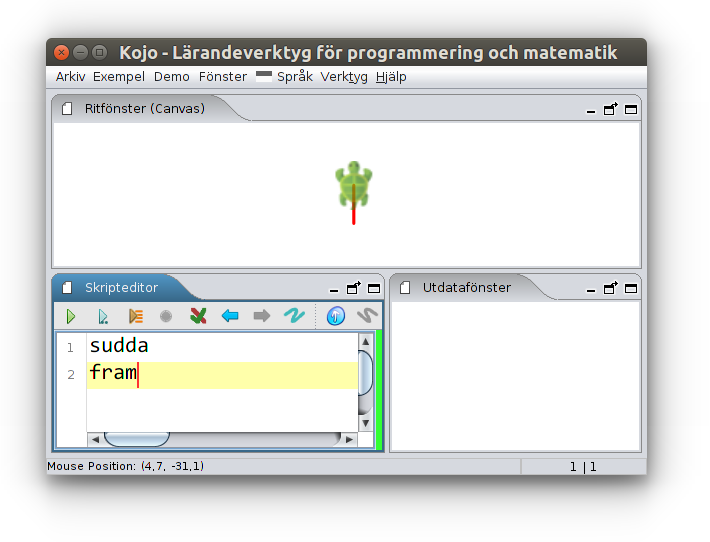
\includegraphics[width=0.8\textwidth]{../img/kojo/kojo.png}
\caption{Den nybörjarvänliga utvecklingsmiljön Kojo för Scala på svenska.}
\label{fig:appendix:ide:kojo}
\end{figure} 

\subsection{Installera Kojo}

Kojo är förinstallerat på LTH:s datorer och körs igång med kommandot \texttt{kojo}. För instruktioner om hur du installerar Kojo på din egen dator se här:\\
\href{http://www.lth.se/programmera/installera/}{lth.se/programmera/installera}

Kojo kräver att \texttt{java} finns på din dator. Eftersom du behöver tillgång till JDK i kursen, är det lika bra att installera hela JDK direkt (och inte bara JRE, så som beskrivs å länken ovan); se vidare hur du gör detta i avsnitt \ref{appendix:compile:install-jdk}. 
%\href{http://www.kogics.net/kojo-download}{www.kogics.net/kojo-download}


\subsection{Använda Kojo}

När du startar Kojo första gången, välj ''Svenska'' i språkmenyn och starta om Kojo. Därefter fungerar grafikfunktionerna på svenska enligt tabell \ref{table:kojo:functions}. När du startat om Kojo inställt på Svenska ser programmet ut ungeför som i figur \ref{fig:appendix:ide:kojo} på sidan \pageref{fig:appendix:ide:kojo}.


Det finns ett antal användbara kortkommando som du hittar i menyerna i Kojo. Undersök speciellt Ctrl+Alt+Mellanslag som ger autokomplettering baserat på det du börjat skriva.


{\small\renewcommand{\arraystretch}{1.45}
\begin{longtable}{@{}p{0.42\textwidth} p{0.55\textwidth}}

\caption{Några av sköldpaddans funktioner. Se även \href{http://lth.se/programmera}{lth.se/programmera}}\label{table:kojo:functions}\\

\emph{Svenska/Engelska} & \emph{Vad händer?}  \\ \hline
\code|sudda| \newline \code|clear| & Ritfönstret suddas \\
\code|fram| \newline \code|forward(25)| & Paddan går framåt 25 steg. \\
\code|fram(100)| \newline \code|forward(100)| & Paddan går framåt 100 steg. \\
\code|höger| \newline \code|right(90)| & Paddan vrider sig 90 grader åt höger. \\
\code|höger(45)| \newline \code|right(45)| & Paddan vrider sig 45 grader åt höger. \\
\code|vänster| \newline \code|left(90)| & Paddan vrider sig 90 grader åt vänster. \\
\code|vänster(45)| \newline \code|left(45)| & Paddan vrider sig 45 grader åt vänster. \\
\code|hoppa| \newline \code|hop| & Paddan hoppar 25 steg utan att rita. \\
\code|hoppa(100)| \newline \code|hop(100)| & Paddan hoppar 100 steg utan att rita. \\
\code|hoppaTill(100, 200)| \newline \code|jumpTo(100, 200)| & Paddan hoppar till läget (100, 200) utan att rita. \\
\code|gåTill(100, 200)| \newline \code|moveTo(100, 200)| & Paddan vrider sig och går till läget (100, 200). \\
\code|hem| \newline \code|home| & Paddan går tillbaka till utgångsläget (0, 0). \\
\code|öster| \newline \code|setHeading(0)| & Paddan vrider sig så att nosen pekar åt höger. \\
\code|väster| \newline \code|setHeading(180)| & Paddan vrider sig så att nosen pekar åt vänster. \\
\code|norr| \newline \code|setHeading(90)| & Paddan vrider sig så att nosen pekar uppåt. \\
\code|söder| \newline \code|setHeading(-90)  | & Paddan vrider sig så att nosen pekar neråt. \\
\code|mot(100,200)| \newline \code|towards(100, 200)| & Paddan vrider sig så att nosen pekar mot läget (100, 200) \\
\code|sättVinkel(90)| \newline \code|setHeading(90)| & Paddan vrider nosen till vinkeln 90 grader. \\
\code|vinkel| \newline \code|heading| & Ger vinkelvärdet dit paddans nos pekar. \\
\code|sakta(5000)| \newline \code|setAnimationDelay(5000) | & Gör så att paddan ritar jättesakta. \\
\code|suddaUtdata| \newline \code|clearOutput| & Utdatafönstret suddas. \\
\code|utdata("hej")| \newline \code|println("hej")| & Skriver texten \texttt{hej} i utdatafönstret. \\
\code|val t = indata("Skriv")| \newline \code|val t = readln("Skriv:")| & Väntar på inmatning efter ledtexten \texttt{Skriv} och sparar den inmatade texten i t.  \\
\code|textstorlek(100)| \newline \code|setPenFontSize(100)| & Paddan skriver med jättestor text nästa gång du gör skriv. \\
\code|båge(100, 90)| \newline \code|arc(100, 90)| & Paddan ritar en båge med radie 100 och vinkel 90. \\
\code|cirkel(100)| \newline \code|circle(radie)| & Paddan ritar en cirkel med radie 100. \\
\code|synlig| \newline \code|visible| & Paddan blir synlig. \\
\code|osynlig| \newline \code|invisible| & Paddan blir osynlig. \\
\code|läge.x| \newline \code|position.x| & Ger paddans x-läge \\
\code|läge.y| \newline \code|position.y| & Ger paddans y-läge \\
\code|pennaNer| \newline \code|penDown| & Sätter ner paddans penna så att den ritar när den går. \\
\code|pennaUpp| \newline \code|penUp| & Sänker paddans penna så att den INTE ritar när den går. \\
\code|pennanÄrNere| \newline \code|penIsDown| & Kollar om pennan är nere eller inte. \\
\code|färg(rosa)| \newline \code|setPenColor(pink)| & Sätter pennans färg till rosa. \\
\code|fyll(lila)| \newline \code|setFillColor(purple)| & Sätter ifyllnadsfärgen till lila. \\
\code|fyll(genomskinlig)| \newline \code|setFillColor(noColor)| & Gör så att paddan inte fyller i något när den ritar. \\
\code|bredd(20)| \newline \code|setPenThickness(20)| & Gör så att pennan får bredden 20. \\
\code|sparaStil| \newline \code|saveStyle| & Sparar pennans färg, bredd och fyllfärg. \\
\code|laddaStil| \newline \code|restoreStyle| & Laddar tidigare sparad färg, bredd och fyllfärg. \\
\code|sparaLägeRiktning| \newline \code|savePosHe| & Sparar pennans läge och riktning \\
\code|laddaLägeRiktning| \newline \code|restorePosHe| & Laddar tidigare sparad riktning och läge \\
\code|siktePå| \newline \code|beamsOn| & Sätter på siktet. \\
\code|sikteAv| \newline \code|beamsOff| & Stänger av siktet. \\
\code|bakgrund(svart)| \newline \code|setBackground(black)| & Bakgrundsfärgen blir svart. \\
\code|bakgrund2(grön,gul)| \newline \code|setBackgroundV(green, yellow)| & Bakgrund med övergång från grönt till gult. \\
\code|upprepa(4){fram; höger}| \newline \code|repeat(4){forward; right}| & Paddan går fram och svänger höger 4 gånger. \\
\code|avrunda(3.99)| & Avrundar 3.99 till 4.0 \\
\code|slumptal(100)| & Ger ett slumptal mellan 0 och 99. \\
\code|slumptalMedDecimaler(100)| & Ger ett slumptal mellan 0 och 99.99999999 \\
\code|systemtid| & Ger nuvarande systemklocka i sekunder. \\
\code|räknaTill(5000)| & Kollar hur lång tid det tar för din dator att räkna till 5000. \\



\hline
\end{longtable}
}%end small

\noindent Scala-koden för den svenska paddans api finns här: \\
\href{https://bitbucket.org/lalit_pant/kojo/src/tip/src/main/scala/net/kogics/kojo/lite/i18n/svInit.scala}{bitbucket.org/lalit\_pant/kojo/src/tip/src/main/scala/net/kogics/\\kojo/lite/i18n/svInit.scala}




\newpage

\section{Eclipse och ScalaIDE}\label{appendix:ide:eclipse}

Eclipse%
\footnote{\href{https://en.wikipedia.org/wiki/Eclipse_(software)}{en.wikipedia.org/wiki/Eclipse\_(software)}}
är en professionell IDE som stödjer många olika programmeringsspråk. Eclipse är skriven i Java och bygger vidare på ett utvecklingsprojekt som initierades av IBM. Eclipse är ett fritt och öppet projekt som numera kontrolleras av en oberoende stiftelse.

Till Eclipse finns en insticksmodul \Eng{plug-in} som kallas ScalaIDE och erbjuder stöd för Scala med tillhörande standardbibliotek.

Eclipse är en omfattande och avancerad programmeringsmiljö med många funktioner och inställningar. Det finns även en omfattande uppsättning insticksmoduler och tilläggsprogram som underlättar utveckling av t.ex. webbprogram, databaser och mycket annat. 

I detta avsnitt ges länkar till installation samt tips om hur du kommer igång med att använda Eclipse och ScalaIDE. Det går ganska snabbt att lära sig grunderna, men det kräven en viss ansträngning att lära sig de mer avancerade funktionerna. Det finns omfattande resurser på nätet som hjälper dig vidare. 


\subsection{Installera Eclipse Mars och ScalaIDE}\label{appendix:ide:eclipse:install}

Eclipse med ScalaIDE är förinstallerat på LTH:s datorer och startas med kommandot \texttt{scalaide} i ett terminalfönster.

ScalaIDE fungerar med Eclipse-versionerna \textit{Luna} och \textit{Mars} (men i skrivande stund fungerar ScalaIDE ännu \textit{inte} med den allra senaste versionen kallad \textit{Neon}). 

För att installera ScalaIDE på din egen dator, följ nedan instruktioner: 

\begin{enumerate}
\item Kontrollera enligt avsnitt \ref{appendix:compile:check-jdk} att du har \texttt{java} installerat och installera vid behov JDK enligt avsnitt \ref{appendix:compile:install-jdk}.

\item Installera Eclipse version \textbf{Mars}, varianten för \textbf{Java Developers} som återfinns på denna sida: \\ \url{https://www.eclipse.org/downloads/packages/release/Mars/2} \\ som är den \textit{andra} varianten i listan (alltså inte Java EE). Följ dessa steg:
\begin{enumerate}
\item Klicka på den \textbf{64-bit}-variant som passar ditt operativsystem.
\item Filen som laddas ner heter något som liknar (beroende på OS): \\ \texttt{eclipse-java-mars-2-win32-x86\_64.zip} 
\\ Det kan ta lång tid att ladda ner filen som är på ca 170MB. Om du klickar på \textit{''select a mirror''} kan du välja en svensk sajt för att ladda ner snabbare. 

\item Dubbelklicka på filen för att packa upp den, vilket kan ta många minuter. Du får, när upppackningen är klar, ett bibliotek med en fungerande Eclipse-installation som du kan placera var du vill. Kör du Windows, lägg den förslagsvis här:\\ 
\code|C:\eclipse\eclipse-java-mars-2-win32-x86_64|

\item för Ubuntu Linux finns kompletterande installationsanvisningar här, som ger dig en ikon i app-menyn m.m.: 
\\ \url{http://askubuntu.com/questions/26632/how-to-install-eclipse}
\end{enumerate}

\item Installera Scala IDE inifrån%
\footnote{Det finns på ScalaIDE-hemsidan möjlighet att ladda ner en Eclipse-variant med färdiginstallerad ScalaIDE-plugin, men då får du i skrivande stund den gamla versionen Eclipse \textit{Luna}, varför du rekommenderas att, enligt instruktionerna här, själv installera ScalaIDE inifrån Eclipse \textit{Mars}, som är den senaste Eclipse-versionen för vilken ScalaIDE fungerar.}
 Eclipse enligt nedan steg:
\begin{enumerate}
\item Starta Eclipse, t.ex. genom att köra igång den exekverbara filen som ligger i underbiblioteket \texttt{eclipse}, i Windows heter den \texttt{eclipse.exe} medan den exekverbara filen i Linux heter \texttt{eclipse} utan filändelse.

\item Välj i frågerutan som dyker upp, någon plats för \textit{workspace} (kvittar vilken just nu, kan ändras senare).

\item Klicka på menyn \textit{Help} $\rightarrow$ \textit{Install new software}.

\item Klicka på \textit{Add}-knappen till höger och skriv: \\ \textit{''ScalaIDE for Scala 2.11''} i \textit{Name}-fältet och ange denna adress i \textit{Location}-fältet: \\
  {\small\mbox{\url{http://download.scala-ide.org/sdk/lithium/e44/scala211/stable/site}}} \\
  och klicka \textit{OK}.
  
\item Du får nu upp en lista med alternativ. Kryssa för alternativet
\\ {\frame{\checkmark}}~~\textit{Scala IDE for Eclipse} \\ och klicka \textit{Next} och sedan \textit{Next} igen och acceptera licensvillkoren och klicka \textit{Finish}.

\item Låt installationen ta sin tid och starta sedan om Eclipse när installationen är färdig. 

\item När Eclipse är igång igen visas en dialog som föreslår att du ska köra \textit{Setup Diagnostics}. Gör detta och välj \textit{Use recommended default settings}. Ändra även i filen \textbf{eclipse.ini} för höja den övre minnesgränsen. Det gör du genom att ändra på den rad i filen som börjar med \texttt{-Xmx}. Hur mycket du ska tillåta som max beror på hur mycket minne du har, men ge minst 1 gigabyte för smidig körning, genom att skriva så här på relevant rad i filen \textbf{eclipse.ini}: \\
\texttt{-Xmx1G } \\


\item Kompletterande information finns här, inklusive en video som visar installationsproceduren och hur man kommer igång med ett ''hello world''-program: \\ \url{http://scala-ide.org/download/current.html}


\end{enumerate}


\end{enumerate}

\noindent I nästa avsnitt beskrivs några rekommenderade anpassningar som du kan göra bland de omfattande inställningsmöjligheterna för Eclipse.

\newpage

\subsection{Anpassa Eclipse och ScalaIDE}\label{subsection:appendix:ide:eclipse:tweaks}

\newcommand\Menu[1]{\textit{#1}}
\newcommand\MenuArrow[1]{\Menu{#1}~$\rightarrow$~}
\newcommand\FramedCheckmark[1]{~\frame{\checkmark}~~\textbf{#1}}
\newcommand\FramedUnchecked[1]{$\Box$~\textbf{#1}}
\newcommand\Button[1]{\fbox{\textbf{#1}}}
\newcommand\EclipsePrefs{\MenuArrow{Window}\MenuArrow{Preferences}}
\newcommand\EclipsePrefsGeneral{\EclipsePrefs\MenuArrow{General}}


Förutom maxminneshöjningen i filen \texttt{eclipse.ini}, som finns i installationskatalogen för Eclipse, till minst \texttt{-Xmx1G } (se föregående avsnitt), är det bra att göra några ytterligare anpassningar av Eclipse och ScalaIDE för att få en snabbare och smidigare utvecklingsmiljö. Du hittar inställningarna i menyn \EclipsePrefs ... uppe till höger i Eclipse-fönstret.



\begin{enumerate}
\item \EclipsePrefsGeneral 
\\ Markera \FramedCheckmark{Show Heap Status} så får du se minnesanvändningen i en liten ruta i nederdelen av fönstret, vilket hjälper dig att upptäcka om minnesbegränsningen i filen \texttt{eclipse.ini} är en flaskhals vid stora projekt och många öppna fönster. Klicka sedan \Button{Apply} längst ner.

\item \label{item:scala-perspective} \EclipsePrefsGeneral\MenuArrow{Editors}\MenuArrow{Perspective}  
\\ Markera \textit{Scala} i listan med perspektiv och klicka på knappen 
 \\ \Button{Make default} till höger och sedan på knappen \Button{Apply} längst ner.

\item \EclipsePrefsGeneral\MenuArrow{Editors}\MenuArrow{TextEditors}
\\ Markera \FramedCheckmark{Insert spaces for tabs} så att du slipper specialtecken som kan tolkas olika av olika editorer. Klicka sedan \Button{Apply} längst ner.

\item \EclipsePrefsGeneral\MenuArrow{Editors}\MenuArrow{TextEditors}
\\ \MenuArrow{Spelling} Avmarkera \FramedUnchecked{Enable spell checking} för att slippa att svenska namn och svenska kommentarer markeras som felstavade. Om du senare jobbar med ett projekt helt på engelska, kan du med fördel markera denna kryssruta igen. Klicka sedan \Button{Apply} längst ner.

\item \EclipsePrefsGeneral\MenuArrow{Editors}\MenuArrow{Webbrowser}
\\ Markera \FramedCheckmark{Use external web browser} för att köra din vanliga webbläsare när du klickar på länkar. Klicka sedan \Button{Apply} längst ner.
  
\item  \EclipsePrefs\MenuArrow{Scala}\MenuArrow{Compile}
\\ I fliken \textbf{Standard} markera dessa kryssrutor för att få extra varningar: \\
\begin{tabular}{l @{}l @{}l}
\textit{deprecation} & \FramedCheckmark{} & varnar vid användning av föråldrad kod som snart utgår \\
\textit{feature}     & \FramedCheckmark{} & påminner om import vid användning av avancerad kod  \\
\textit{unchecked}   & \FramedCheckmark{} & ger tips vid speciella problem med generiska typer \\
\end{tabular}\\
och klicka sedan på knappen \Button{Apply} längst ner.

\item \EclipsePrefs\MenuArrow{Java}\MenuArrow{Compiler}\MenuArrow{Errors/Warnings}
\\ Veckla ut listan \textbf{Potential programming problems} och sätt \textbf{Resource leak} till alternativet \textbf{Ignore}, så slipper du varningar vid användning \jcode{Scanner} i Java. Klicka sedan \Button{Apply} längst ner.

\end{enumerate}

\noindent Ovan anpassningar är rekommenderade men inte nödvändiga och du kan gärna välja att göra andra anpassningar som passar just dig. Skriv då gärna ner vilken inställning du ändrat, så att du hittar tillbaka om du ångrar dig. 

Du hittar tips om fler inställningar för att anpassa ScalaIDE här: \\
\url{http://scala-ide.org/docs/current-user-doc/advancedsetup}



\subsection{Använda Eclipse och ScalaIDE}\label{appendix:ide:eclipse:use}

Ett grundläggande koncept i Eclipse är \textbf{workspace}. Ett workspace utgör ett arbetsområde kopplat till en katalog i ditt filsystem där du kan arbeta med ett eller flera \textbf{projekt}. Ett projekt innehåller i sin tur dina källkodsfiler och klassfiler etc. i en specifik katalogstruktur som Eclipse skapar när du editerar, kompilerar och kör dina projekt. 

\subsubsection{Starta och välja workspace}\label{subsubsection:start:eclipse}

När du startar Eclipse måste du välja vilket workspace du vill använda innan du kommer vidare. När du kör igång Eclipse första gången, klicka OK enligt det förslag som ges. Du kan senare växla workspace genom menyn \MenuArrow{File}\Menu{Switch Workspace}. Om katalogen du anger inte redan finns, kommer den att skapas och initieras med de filer Eclipse behöver.

I figur \ref{fig:appendix:eclipse:welcome} visas välkomstfliken i Eclipse med sina länkar till funktionsöversikt och olika handledningar. Stäng välkomstfliken genom att klicka på flikens kryss eller på ikonen \textit{Workbench}. Då kommer du vidare till den normala arbetsytan i Eclipse. Du kan få tillbaka välkomstfliken igen via menyn \MenuArrow{Help}\Menu{Welcome}. 

\begin{figure}[H]
\centering
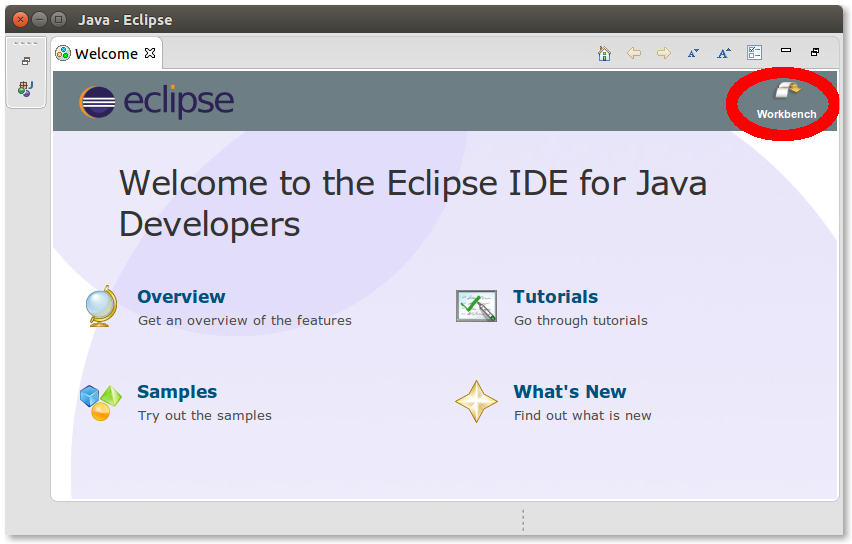
\includegraphics[width=1.0\textwidth]{../img/eclipse/eclipse-welcome.png}
\caption{Välkomstfliken för Eclipse, som nås via menyn \MenuArrow{Help}\Menu{Welcome}. Gå vidare genom att klicka på \textit{Workbench}.}
\label{fig:appendix:eclipse:welcome}
\end{figure}

\subsubsection{Välja perspektiv och visa olika vyer}

Eclipse-fönstret kan innehålla många underfönster i olika flikar, så kallade \textbf{views} eller vyer, som kan arrangeras på olika vis efter hur du vill ha dem. Vilka vyer som syns och hur de placeras beror på vilket s.k. \textbf{perspective} som är aktivt.  Figur \ref{fig:appendix:eclipse:open-perspective} visar arbetsytan med olika vyer i Java-perspektivet. 

Du kan byta till Scala-perspektivet genom att trycka på 
\includegraphics[scale=0.75]{../img/eclipse/eclipse-perspective-button.png} eller genom menyn \MenuArrow{Window}\MenuArrow{Perspective}\MenuArrow{Open Perspective}\MenuArrow{Other...}\Menu{Scala}.
Du kan anpassa inställningarna så att Scala blir \textit{default perspective}, se steg \ref{item:scala-perspective} i avsnitt \ref{subsection:appendix:ide:eclipse:tweaks} på sidan \pageref{subsection:appendix:ide:eclipse:tweaks}.

Stäng vyerna \textit{Task List} och \textit{Outline} om du vill ha mer plats till de övriga vyerna för paketnavigering, editering och utdata. Du kan öppna stängda vyer igen genom menyn \MenuArrow{Window}\Menu{Show View}. 

\begin{figure}
\centering
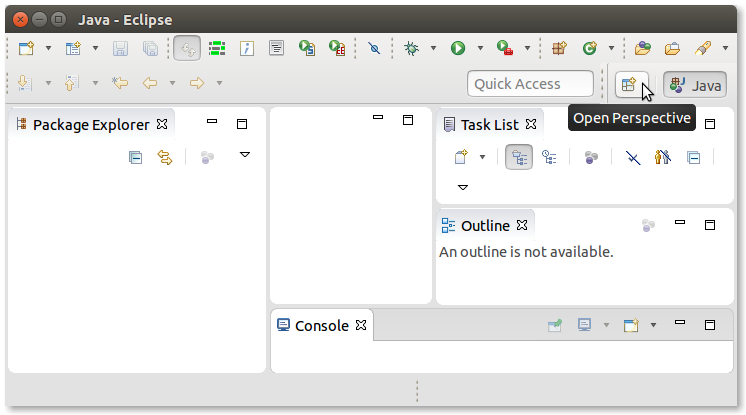
\includegraphics[width=1.0\textwidth]{../img/eclipse/eclipse-open-perspective.png}
\caption{Arbetsytan i Eclipse. Du kan växla mellan Scala- och Java-perspektivet genom att klicka på perspektivvalsknappen.}
\label{fig:appendix:eclipse:open-perspective}
\end{figure}

\subsubsection{Hello World}\label{subsubsection:eclipse:hello-world}

Efter att du öppnat Eclipse med ScalaIDE i ett tomt workspace och valt Scala-perspektivet enligt föregående avsnitt, kan du skapa ditt första projekt med ett \textit{''Hello World''}-program enligt stegen nedan.

\begin{enumerate}
\item Högerklicka i \Menu{Package Explorer} och välj \MenuArrow{New}\Menu{Scala Project}, varefter en dialogruta visas. 

\item Fyll i namnet \texttt{hello} i fältet \Menu{Project Name} och klicka \Button{Finish}.

\item Högerklicka igen i \Menu{Package Explorer} och välj \MenuArrow{New}\Menu{Scala Object}, varefter en ny dialogruta visas. 

\item Fyll i namnet \texttt{hi} i fältet \Menu{Project Name} och klicka \Button{Finish}.

\item Du får nu i editorvyn ett kodskellet med \code{object hi}.

\item Börja skriv \code{main} som visas i figur \ref{fig:appendix:eclipse:complete-main} och tryck Ctrl+Mellanslag för att aktivera kodkomplettering \Eng{code completion}. Då får du upp en lista med alternativ. Välj det översta alternativet \texttt{main} varefter ett kodskellet med en main-metod klistras in automatiskt i din kod.

\begin{figure}
\centering
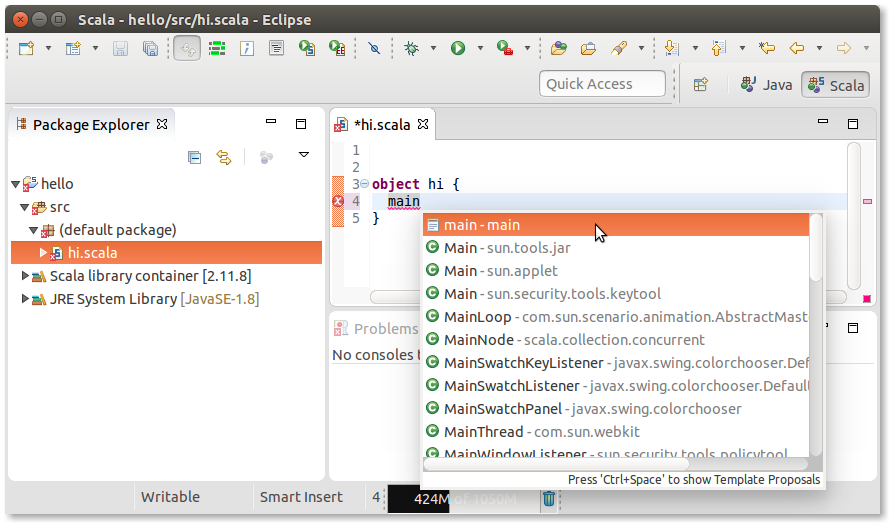
\includegraphics[width=1.0\textwidth]{../img/eclipse/eclipse-complete-main.png}
\caption{Aktivera kodkomplettering med Ctrl+Mellanslag efter ordet \code{main}.}
\label{fig:appendix:eclipse:complete-main}
\end{figure}

\item Fyll i lämplig utskriftstext i ett \code{println}-anrop så att din \code{main}-metod blir så som visas i editorfliken i figur \ref{fig:appendix:eclipse:hello-world}.

\begin{figure}[H]
\centering
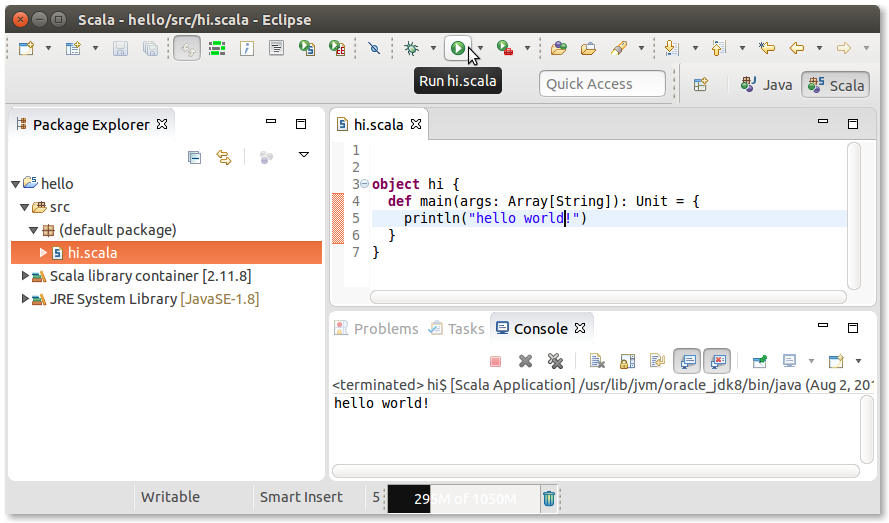
\includegraphics[width=1.0\textwidth]{../img/eclipse/eclipse-hello-world.png}
\caption{Skriv klart \code{main}-metoden och kör ditt program med play-knappen.}
\label{fig:appendix:eclipse:hello-world}
\end{figure}

\item Kör ditt program genom att trycka på den gröna play-knappen, som muspekaren i figur \ref{fig:appendix:eclipse:hello-world} pekar på. Du kan också trycka F11 för att köra igång din app, efter att du vid första körningen i dialogen \textit{Select Preferred Launcher} markerat  \FramedCheckmark{Use configuration specific settings} och valt alternativet \textit{Scala Application (new debugger) Launcher}. 

\end{enumerate}




\subsubsection{Ladda ner kursens workspace och importera i Eclipse}

Det finns en zip-fil med ett workspace med projekt för flera av kursens laborationer som du kan ladda ner och importera i Eclipse. Följ stegen nedan.

\begin{enumerate}
\item Ladda ner kursens workspace här: \url{http://cs.lth.se/pgk/ws}

\item Packa upp filen på lämpligt ställe.

\item Starta Eclipse med ScalaIDE-plugin (se startinstruktioner på sidan \pageref{subsubsection:start:eclipse}). 

\item Växla workspace till biblioteket du nyss packade upp, ungefär som i figur \ref{fig:eclipse:ide:open} och klicka \Button{OK}.

\begin{figure}[H]
\centering
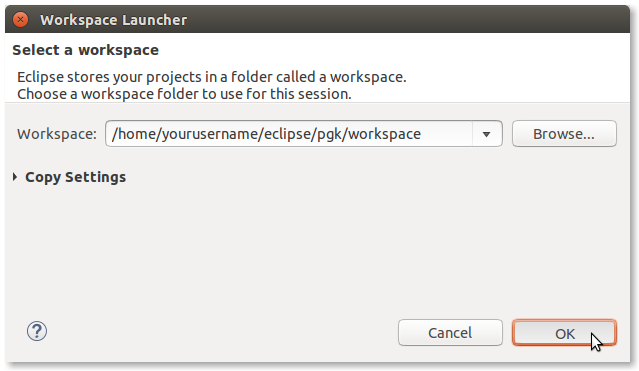
\includegraphics[width=1.0\textwidth]{../img/eclipse/eclipse-select-workspace.png}
\caption {Öppna kursens workspace genom att bläddra till biblioteket där du packade upp filen som du laddat ned från: \url{http://cs.lth.se/pgk/ws} }
\label{fig:eclipse:ide:open}
\end{figure}

\item Stäng välkomstfliken för att komma vidare till workbench (se figur \ref{fig:appendix:eclipse:welcome} på sidan \pageref{fig:appendix:eclipse:welcome}). Det ser då ut ungefär som i figur~\ref{fig:appendix:eclipse:open-perspective} på sidan \pageref{fig:appendix:eclipse:open-perspective}. Det syns ännu inget i \textit{Package Explorer} då vi ännu inte importerat något projekt. 

\item Innan du går vidare, säkerställ att du har Scala-perspektivet aktiverast. Du kan växla till Scala-perspektivet genom att trycka på 
\includegraphics[scale=0.75]{../img/eclipse/eclipse-perspective-button.png} eller genom menyn \MenuArrow{Window}\MenuArrow{Perspective}\MenuArrow{Open Perspective}\MenuArrow{Other...}\Menu{Scala}.
Du kan anpassa inställningarna så att Scala blir \textit{default perspective}, se steg \ref{item:scala-perspective} i avsnitt \ref{subsection:appendix:ide:eclipse:tweaks} på sidan \pageref{subsection:appendix:ide:eclipse:tweaks}.


\item Högerklicka i \textit{Package Explorer} och välj \Menu{Import...}, se Fig.~\ref{fig:eclipse:import}, eller välj menyn \MenuArrow{File}\Menu{Import...}. 

\begin{figure}[H]
\centering
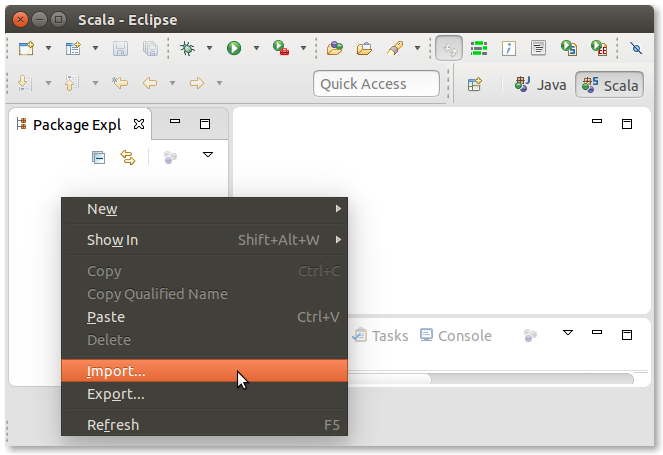
\includegraphics[width=1.0\textwidth]{../img/eclipse/eclipse-import.png} 
\caption {Välj \Menu{Import}-menyn för att importera existerande projekt.}
\label{fig:eclipse:import}
\end{figure}

\item Nu öppnas \Menu{Import}-dialogen som visas i figur \ref{fig:eclipse:import-existing}. Öppna mappen \Menu{General}, markera \textbf{Existing Projects into Workspace} och klicka \Button{Next}.



\begin{figure}[H]
\centering
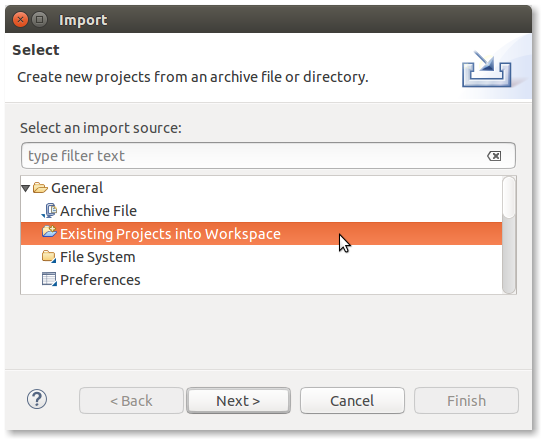
\includegraphics[width=0.75\textwidth]{../img/eclipse/eclipse-import-existing.png} 
\caption {Välj att importera existerande projekt under \Menu{General}.}
\label{fig:eclipse:import-existing}
\end{figure}


\begin{figure}[H]
\centering
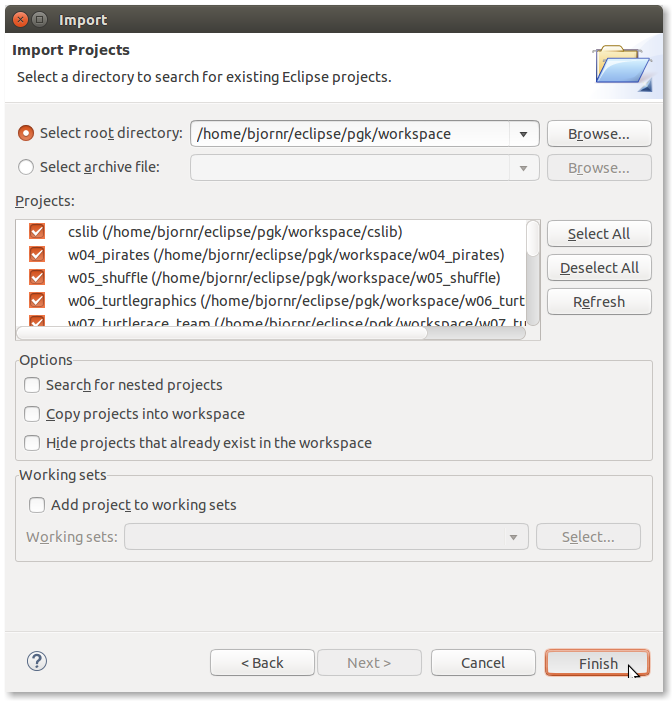
\includegraphics[width=1.0\textwidth]{../img/eclipse/eclipse-import-projects.png} 
\caption {Välj \FramedCheckmark{Select Root Directory} och klicka \Button{Browse}.}
\label{fig:eclipse:import-projects}
\end{figure}


\item Nu kommer ytterligare ett dialogfönster som visas i figure \ref{fig:eclipse:import-projects}. Med \FramedCheckmark{Select Root Directory} markerad kan du klicka \Button{Browse} för att ange workspace-mappen i ännu en dialog där du bara ska trycka \Button{Ok} utan att välja underbibliotek till workspace. När det är klart ska det se ut som i figur \ref{fig:eclipse:import-projects} där alla Eclipse-projekt \FramedCheckmark{cslib}, \FramedCheckmark{w04\_pirates}, etc. är markerade. Klicka sedan \Button{Finish}.

\item Följ ''Hello World''-instruktionerna på sidan \pageref{subsubsection:eclipse:hello-world} och skapa programmet som visas i figure \ref{fig:eclipse:pirates-hi}, genom att veckla ut projektet \textbf{w04\_pirates}, markera och högerklicka på paketet \textbf{priates}, och välja \MenuArrow{New}\Menu{Scala Object}.

\item Om du får problem, fråga någon som känner till Eclipse om hjälp. Det finns även mycket hjälp på nätet, se till exempel: \\ \href{http://stackoverflow.com/questions/8522149/eclipse-not-recognizing-scala-code}{stackoverflow.com/questions/8522149/eclipse-not-recognizing-scala-code}

\begin{figure}[H]
\centering
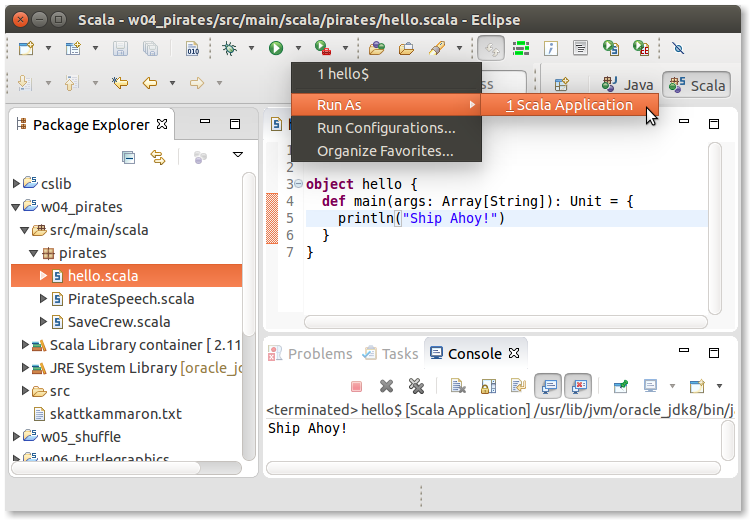
\includegraphics[width=1.0\textwidth]{../img/eclipse/eclipse-pirates-hello.png} 
\caption {Skapa ett \MenuArrow{New}\Menu{Scala Object} med kod enligt bilden.}
\label{fig:eclipse:pirates-hi}
\end{figure}


\end{enumerate}



\newpage

\section{IntelliJ IDEA}\label{appendix:ide:intellij}

IntelliJ IDEA%
\footnote{\href{https://en.wikipedia.org/wiki/IntelliJ_IDEA}{en.wikipedia.org/wiki/IntelliJ\_IDEA}}
 är en professionell IDE som stödjer många olika programmeringsspråk. IntelliJ är skriven i Java och utvecklas av det tjeckiska företaget JetBrains. 

IntelliJ IDEA finns i två varianter: en gratis gemenskapsvariant med öppenkällkodslicens \Eng{Community edition}, samt en betalvariant med sluten källkod och support-tjänster.


Till IntelliJ IDEA finns en insticksmodul \Eng{plug-in} som erbjuder stöd för Scala med tillhörande standardbibliotek..

IntelliJ IDEA är en omfattande och avancerad programmeringsmiljö med många funktioner och inställningar. Det finns även en omfattande uppsättning insticksmoduler och tilläggsprogram som underlättar utveckling av t.ex. webbprogram, databaser och mycket annat. 

I detta avsnitt ges länkar till installation samt tips om hur du kommer igång med att använda IntelliJ IDEA med Scala. Det går ganska snabbt att lära sig grunderna, men det kräven en viss ansträngning att lära sig de mer avancerade funktionerna. Det finns omfattande resurser på nätet som hjälper dig vidare. 

Google tillkännagav 2013 att företaget övergår från Eclipse till IntelliJ som den officiellt understödda utvecklingsmiljön för Android och 2014 lanserades utvecklingsmiljön AndroidStudio%
\footnote {\href{https://en.wikipedia.org/wiki/Android_Studio}{en.wikipedia.org/wiki/Android\_Studio}}
 som bygger vidare på IntelliJ. 

\subsection{Installera IntelliJ med Scala}\label{appendix:ide:intellij:install}

IntelliJ med Scala-plug-in är förinstallerat på LTH:s datorer och startas med kommandot \texttt{idea} i ett terminalfönster.

\begin{itemize}
\item För Ubuntu Linux finns ett färdigt paket som du kan installera med dessa kommandon i terminalen: 
\begin{REPLnonum}
sudo add-apt-repository ppa:mmk2410/intellij-idea-community
sudo apt-get update
\end{REPLnonum}
Mer information om denna ppa finns här:\\ \url{https://launchpad.net/~mmk2410/+archive/ubuntu/intellij-idea-community}\item För Windows och Mac: ladda ner och kör installationsfil för ditt operativsystem för den öppna varianten kallad \textbf{Community} här: \\
\url{https://www.jetbrains.com/idea/download/} \\
Följ instruktionerna som ges av installationsprogrammet.
\end{itemize}

\subsection{Anpassa IntelliJ}\label{appendix:ide:intellij:tweak}
Första gången du kör igång IntelliJ får du ett antal frågor om vilka anpassningar du vill göra. Följ instruktionerna steg för steg enligt nedan.
\begin{enumerate}
\item \textbf{UI Theme}. Denna dialog gäller utseende på gränssnittet. Det tema som kallas \textit{Dracula} är en populär variant med nedtonade färger anpassade för att vara skonsamma mot ögonen. Klicka \Button{Next} när du valt tema.

\item \textbf{Default plugins}. Denna dialog gäller inställningar av befintliga insticksmoduler. Dessa inställningar fungerar bra som de är. Klicka \Button{Next}.

\item \textbf{Featured plugins}. I rutan för \textbf{Plugin for Scala language support} Klicka \Button{Install} och låt installationen av Scala fullbordas. 

\item Klicka därefter \Button{Start using IntelliJ IDEA}.

\item I välkomstfönstrets nedre hörn, välj \MenuArrow{Configure}\Menu{Settings} och överväg om du vill göra följande lämpliga men ej nödvändiga inställningar. 
\begin{enumerate}
\item I fliken \MenuArrow{Editor}\Menu{General} markera \FramedCheckmark{Change font size (Zoom) with Ctrl+Mouse Wheel} för att lätt kunna ändra textstorlek i editorn. Klicka \Button{Apply} nere till höger.

\item I fliken \MenuArrow{Editor}\Menu{Inspections} och välj \Menu{Spelling} i högra listan. Avmarkera \FramedUnchecked{Typo} för att undvika att svenska ord blir markerade som felstavade. Klicka \Button{Apply} nere till höger.

\item I fliken \MenuArrow{Editor}\Menu{File and Code Templates} och under fliken \Menu{Files} i högra listan: för varje Scala-filtyp (Scala Class, Scala Trait, Scala Object, ...) ta bort de initiala raderna i mallen som börjar med \code{#} för att slippa onödiga kommentarer i koden när du skapar nya filer. Klicka \Button{Apply} nere till höger.
 
\end{enumerate} 
Du kan också göra ovan och liknande anpassningar senare genom menyn \MenuArrow{File}\Menu{Settings...}
\end{enumerate} 

\subsection{Använda IntelliJ}\label{appendix:ide:intellij:use}

\subsubsection{Skapa ett nytt projekt}

När du startar IntelliJ IDEA utan förvalt projekt visas välkomstskärmen i figur \ref{fig:idea:welcome}. Klicka på \Menu{Create New Project}, varefter dialogen i figur \ref{fig:idea:new-project} visas. Följ stegen enligt nedan.

\begin{figure}[H]
\centering
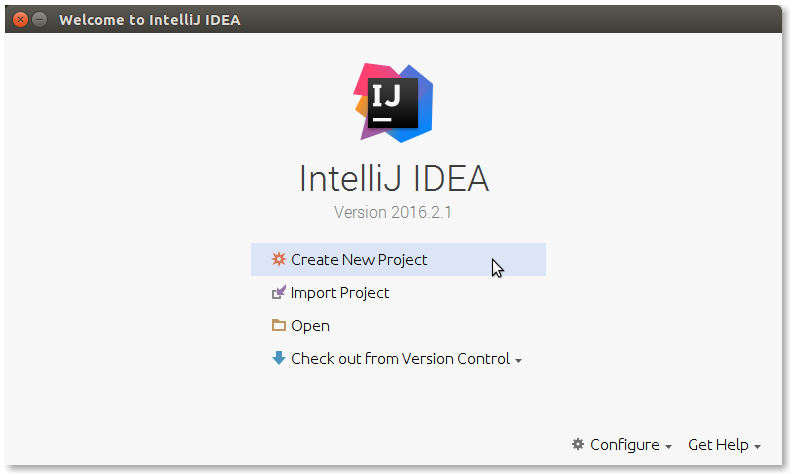
\includegraphics[width=0.8\textwidth]{../img/intellij/idea-welcome.png} 
\caption{Välkomstfönstret för IntelliJ IDEA.}
\label{fig:idea:welcome}
\end{figure}

\begin{enumerate}
\item I dialogen \textbf{New Project} ska du ge projektet ett namn och välja körmiljö för ditt projekt. Ge projektet namnet \texttt{hello} enligt figur \ref{fig:idea:new-project}. 

\item Välj sedan att skapa ett Scala-projekt genom att markera \textbf{Scala} enligt figur \ref{fig:idea:new-scala-project} och klicka \Button{Next}.

\begin{figure}[H]
\centering
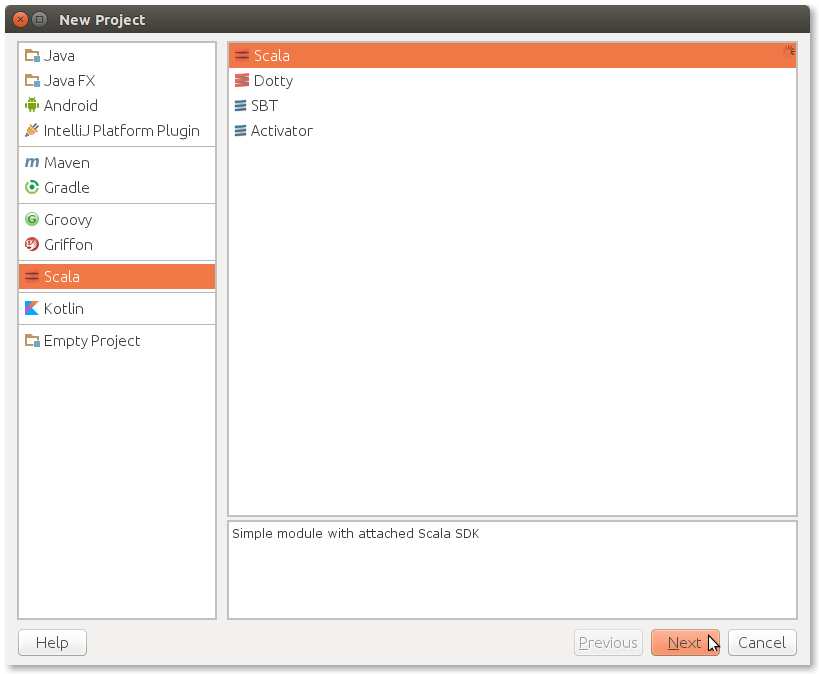
\includegraphics[width=0.65\textwidth]{../img/intellij/idea-new-scala-project.png} 
\caption{Välj att skapa ett Scala-projekt.}
\label{fig:idea:new-scala-project}
\end{figure}

\item Välj sedan \textbf{Project SDK} genom att klicka på \Button{New...}, välja \textit{JDK} och sedan veckla ut fliken \textit{JVM} och  välja \code{Oracle_jdk8} och klicka \Button{OK} enligt  figur \ref{fig:idea:new-project}.

\item Välj sedan \textbf{Scala SDK} genom att klicka på \Button{Create...}, markera raden med \textit{System 2.11.8} och klicka \Button{OK} enligt  figur \ref{fig:idea:new-project}.

\item Avsluta med att klicka \Button{Finish} i dialogen \textbf{New Project}.

\begin{figure}[H]
\centering
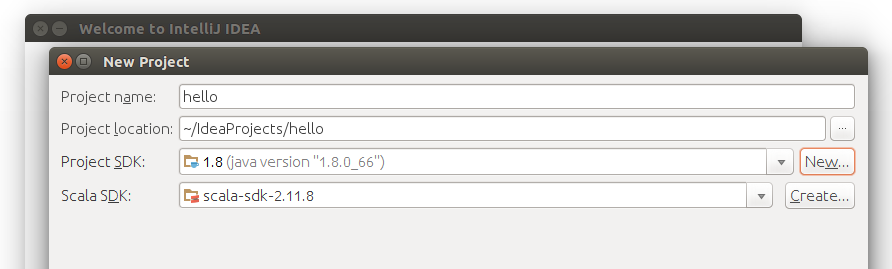
\includegraphics[width=1.0\textwidth]{../img/intellij/idea-new-project.png} 

\begin{minipage}{0.27\textwidth}
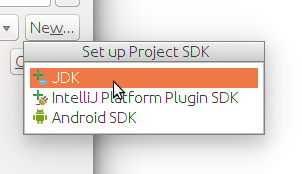
\includegraphics[width=1.0\textwidth]{../img/intellij/idea-project-sdk-jvm.png} 
\end{minipage}
\begin{minipage}{0.35\textwidth}
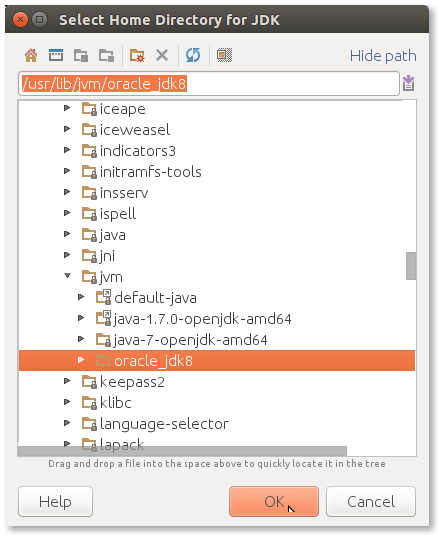
\includegraphics[width=1.0\textwidth]{../img/intellij/idea-project-sdk-home.png} 
\end{minipage}
\begin{minipage}{0.35\textwidth}
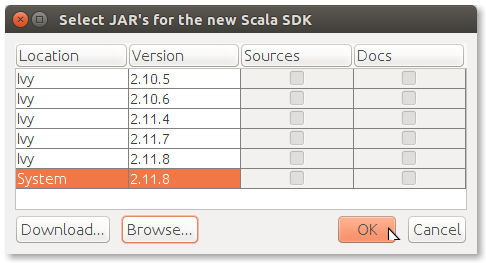
\includegraphics[width=1.0\textwidth]{../img/intellij/idea-scala-sdk.png} 
\end{minipage}%

\caption{Namnge ditt projekt och ställ in körmiljön för JVM och Scala genom att klicka på \Button{New...} och \Button{Create...}}.
\label{fig:idea:new-project}
\end{figure}

\item Du får nu ett projektfönster som liknar det i figur \ref{fig:idea:project-hello} på sidan \pageref{fig:idea:project-hello}.


\begin{figure}
\centering
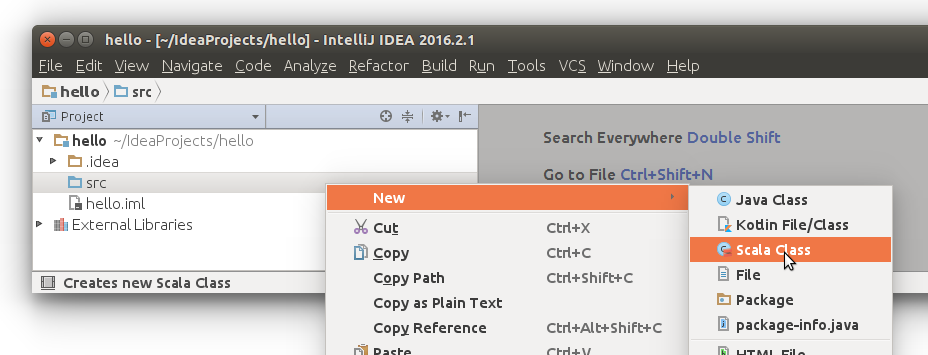
\includegraphics[width=1.0\textwidth]{../img/intellij/idea-new-scala-class.png} 

\begin{minipage}{0.35\textwidth}
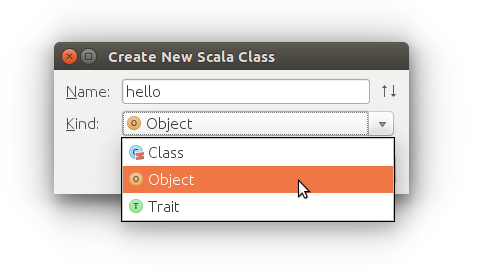
\includegraphics[width=1.0\textwidth]{../img/intellij/idea-scala-object.png} 
\end{minipage}
\begin{minipage}{0.60\textwidth}
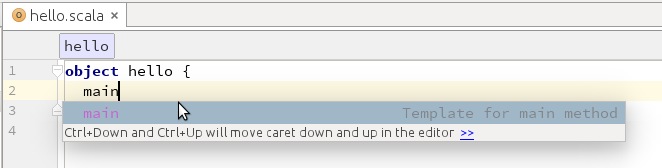
\includegraphics[width=1.0\textwidth]{../img/intellij/idea-complete-main.png} 
\end{minipage}%

\caption{Högerklicka på mappen \textbf{src} och välj \MenuArrow{New}\Menu{Scala Class} och skapa ett nytt Scala-objekt med main-metod. Aktivera kodkomplettering i editorn efter ordet main med TAB.}
\label{fig:idea:project-hello}
\end{figure}


\item Veckla ut ditt projekt och högerklicka på \texttt{src} och välj \MenuArrow{New}\Menu{Scala Class}.Välj sedan \textbf{Object} i dialogen \textbf{Create New Scala Class} och klicka \Button{OK}, enligt figur \ref{fig:idea:project-hello}.

\item Du får nu upp ett editorfönster med koden för objektet \code{hello}. Skriv ordet \code{main} inuti objektet och tryck TAB för att aktivera kodkomplettering. En mall för main-metoden klistras då in i objektet. 

\item Skriv kod så att det ser ut som i editorfönstret i figur \ref{fig:idea:hello-world} på sidan \pageref{fig:idea:hello-world}.

\item Kör igång ditt program genom att klicka på play-knappen eller genom att trycka Shift+F10. Om play-knappen är initialt är grå i stället för grön, välj menyn \MenuArrow{Run}\Menu{Run...}. 

\end{enumerate}


\noindent Mer information om hur du använder Scala-plugin för IntelliJ finns här:\\
\href{https://confluence.jetbrains.com/display/SCA/Scala+Plugin+for+IntelliJ+IDEA}{confluence.jetbrains.com/display/SCA/Scala+Plugin+for+IntelliJ+IDEA}

\begin{figure}
\centering
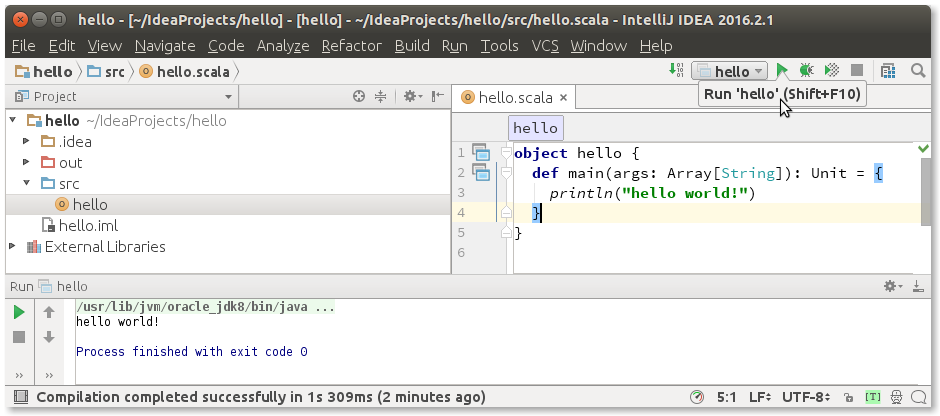
\includegraphics[width=1.0\textwidth]{../img/intellij/idea-hello.png} 
\caption{Kör ditt program med play-knappen eller \MenuArrow{Run}\Menu{Run...}.}
\label{fig:idea:hello-world}
\end{figure}


\subsubsection{Ladda ner kursens workspace och importera i IntelliJ IDEA}

Det finns en zip-fil med ett workspace med projekt för flera av kursens laborationer som du kan ladda ner och importera i Eclipse. Följ stegen nedan.

\begin{enumerate}
\item Ladda ner kursens workspace här: \url{http://cs.lth.se/pgk/ws}

\item Packa upp filen på lämpligt ställe.

\item Starta IntelliJ. Om du redan har ett projekt igång välj menyn \MenuArrow{File}\Menu{Close project} så kommer du tillbaka till välkomstfönstret. Välj \textbf{Import Project} så som visas i figure \ref{fig:idea:import1-project}.

\begin{figure}[H]
\centering
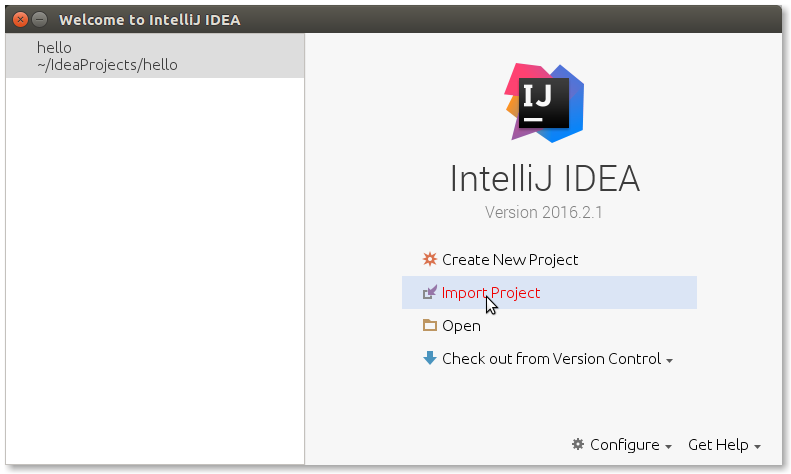
\includegraphics[width=1.0\textwidth]{../img/intellij/idea-import1-project.png} 
\caption{Välj \Menu{Import Project} efter att du stängt ev. öppna projekt.}
\label{fig:idea:import1-project}
\end{figure}

\item Bläddra dit du packat upp workspace och markera denna folder i likhet med figur \ref{fig:idea:import23-select} och klicka \Button{OK}. I den efterföljande dialogen välj \textbf{Eclipse} och klicka \Button{Next}.

\item Klicka \Button{Next} igen i dialogen som liknar figur \ref{fig:idea:import4-directory} på sidan \pageref{fig:idea:import4-directory}, där mappen du valt är förvald.

\item Klicka \Button{Next} igen enligt figur \ref{fig:idea:import5-select-projects} på sidan  \pageref{fig:idea:import5-select-projects}. Alla tillgängliga Eclipse-projekt ska vara markerade.

\item Klicka \Button{Finish} enligt figur \ref{fig:idea:import5-select-projects} med förifylld text oförändrad.

\item Bläddra fram filen \texttt{PirateSpeech.scala} och öppna den med ett dubbelklick. Klicka på länken \textbf{Setup Scala SDK} uppe till höger enligt figur \ref{fig:idea:import78-setup-scala-sdk} på sidan \pageref{fig:idea:import78-setup-scala-sdk}. I efterföljande dialog kontrollera att \texttt{scala-sdk-2.11.8} är förvalt och klicka \Button{OK}.

\item Lägg till testutskrift enligt rad 7 i figur \ref{fig:idea:import9-run} på sidan \pageref{fig:idea:import9-run}. Testkör genom att välja menyn \MenuArrow{Run}\Menu{Run..} eller tryck Alt+Shift+F10 och sedan välja \code{PirateSpeech}. Kontrollera att utskriften i utskriftsfönstret ser ut som förväntat.
\end{enumerate}

\noindent Om du får problem på vägen, be någon med erfarenhet av IntelliJ om hjälp.


{\vfill
\begin{figure}[H]
\centering
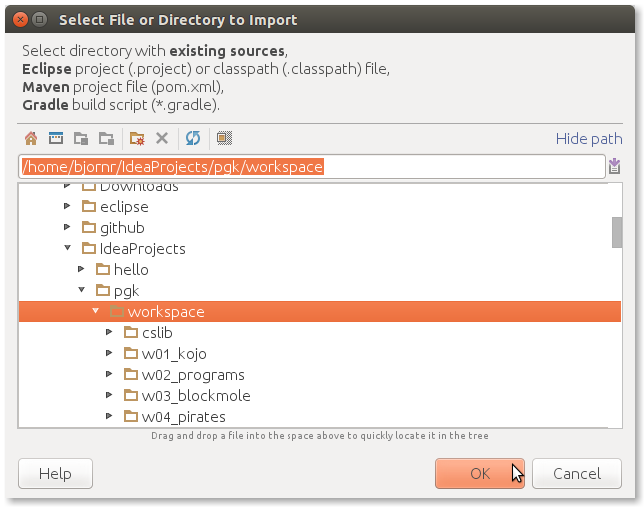
\includegraphics[width=1.0\textwidth]{../img/intellij/idea-import2-select.png} 

{\hfill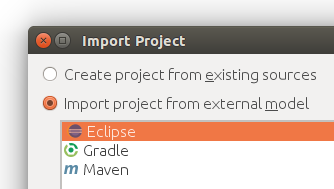
\includegraphics[width=0.4\textwidth]{../img/intellij/idea-import3-eclipse.png}} 

\caption{Markera den upp-packade workspace-mappen från zip-filen som du laddat ner från: \url{http://cs.lth.se/pgk/ws} och välj \textbf{Eclipse}-import.}
\label{fig:idea:import23-select}
\end{figure}
}

\begin{figure}
\centering
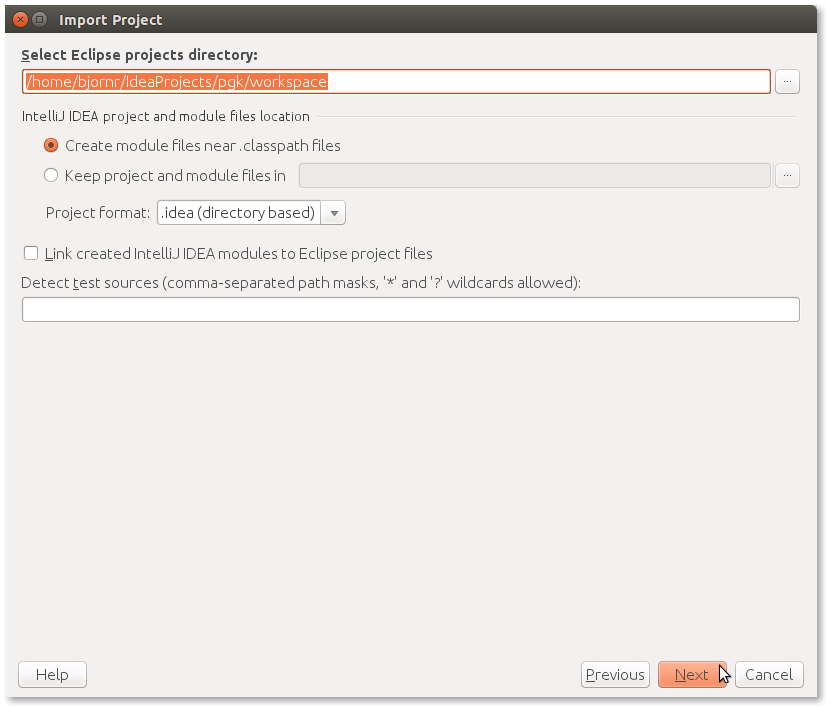
\includegraphics[width=0.85\textwidth]{../img/intellij/idea-import4-directory.png} 
\caption{Klicka \Button{Next} med förvalda alternativ oförändrade.}
\label{fig:idea:import4-directory}
\end{figure}

\begin{figure}
\centering
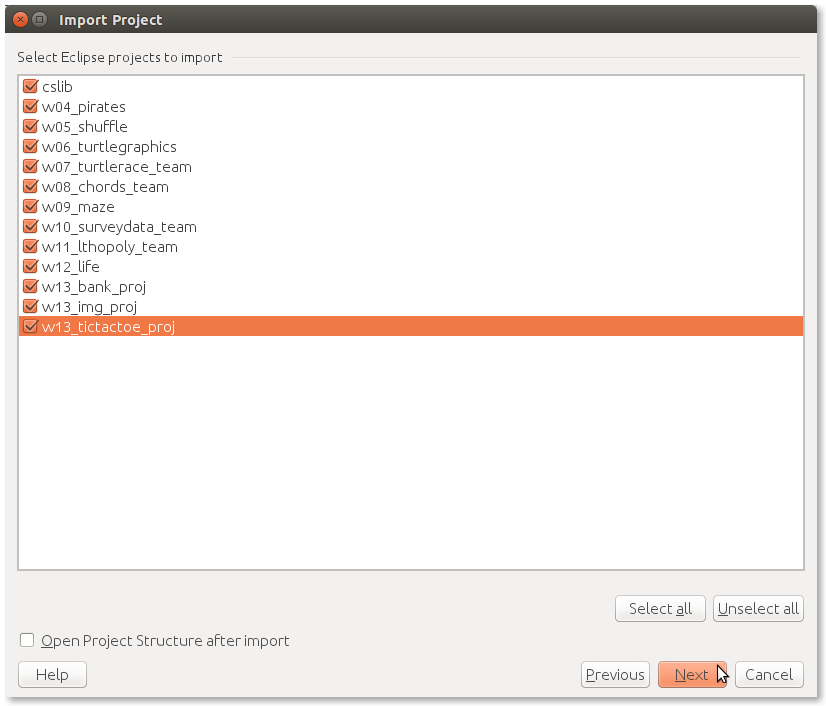
\includegraphics[width=0.85\textwidth]{../img/intellij/idea-import5-select-projects.png} 
\caption{Klicka \Button{Next} med alla projekt markerade.}
\label{fig:idea:import5-select-projects}
\end{figure}

\begin{figure}
\centering
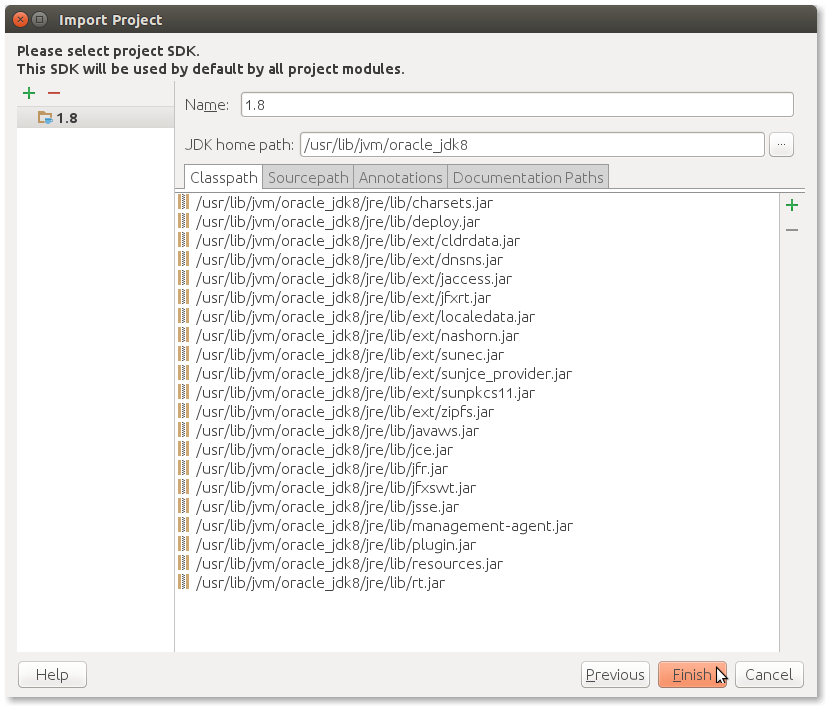
\includegraphics[width=0.8\textwidth]{../img/intellij/idea-import6-select-SDK.png} 
\caption{Klicka \Button{Finish} med förifyllda fält oförändrade.}
\label{fig:idea:import6-select-SDK}
\end{figure}

\begin{figure}
\centering
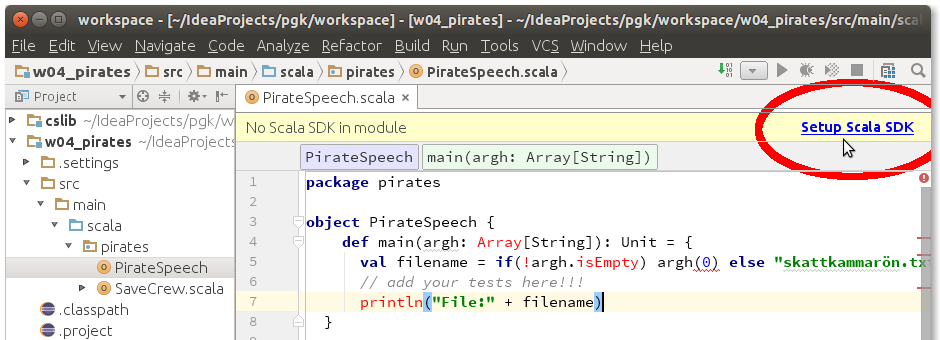
\includegraphics[width=1.0\textwidth]{../img/intellij/idea-import7-setup-scala-sdk.png} 

\vspace{1em}{\hfill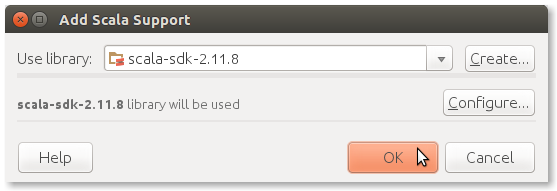
\includegraphics[width=0.6\textwidth]{../img/intellij/idea-import8-add-scala-support.png}} 
\caption{Bläddra fram PirateSpeech.scala i projektet \code{w04_pirates} och klicka på länken \textbf{Setup Scala SDK} och klicka \Button{OK} i efterföljande dialog.}
\label{fig:idea:import78-setup-scala-sdk}
\end{figure}

\begin{figure}
\centering
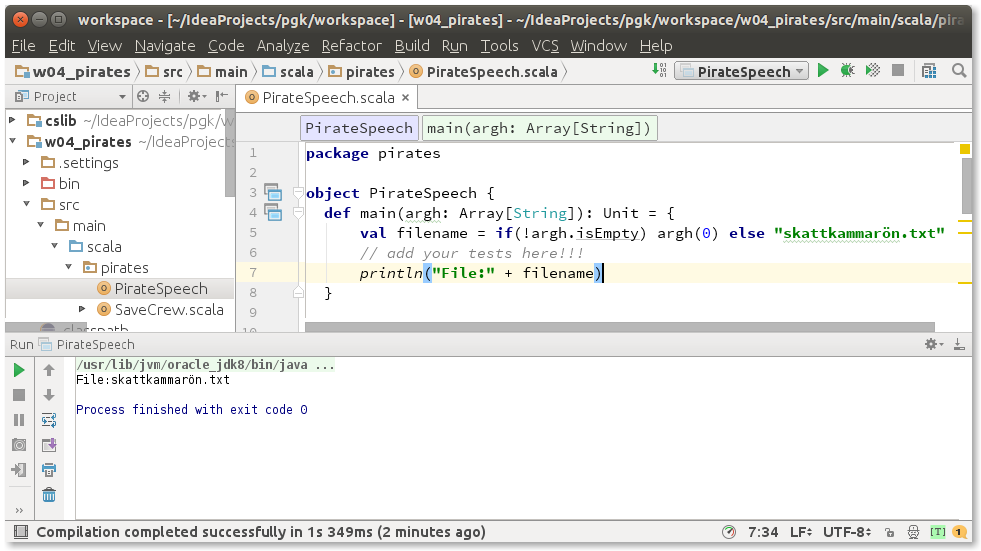
\includegraphics[width=1.0\textwidth]{../img/intellij/idea-import9-run.png} 
\caption{Lägg till utskriften i bilden ovan på rad7. Testkör genom att välja menyn \MenuArrow{Run}\Menu{Run..} (eller trycka Alt+Shift+F10) och sedan välja \code{PirateSpeech}. Observera utskriften i utskriftsfönstret.}
\label{fig:idea:import9-run}
\end{figure}





\input{postchapters/scalajs.tex}
\input{postchapters/android.tex}

\part{Lösningar}

\setcounter{chapter}{11} %next is L in \Alph
\chapter{Lösningar till övningarna}\label{chapter:solutions}
\setcounter{section}{7}

\PreSolutionfalse

\let\QUESTBEGIN\ifPreSolution  % to mark formatting and numbering of exercises
\let\SOLUTION\else  % to mark solutions in the same file as questions
\let\QUESTEND\fi    % to mark end of exercise

%!TEX encoding = UTF-8 Unicode

%!TEX root = ../compendium2.tex

\Exercise{\ExeWeekEIGHT}\label{exe:W08}

\begin{Goals}
\item Kunna skapa och använda matriser med nästlade strukturer av \code{Vector}.
\item Kunna iterera över elementen i en matris med nästlade \code{for}-satser och \code{for}-\code{yield}-uttryck, samt nästlad applicering av \code{map} respektive \code{foreach}.
\item Kunna skapa och använda funktioner som tar matriser som parametrar.
\item Känna till generiska funktioner.
\item Känna till generiska klasser.
\item Kunna skapa och använda matriser med hjälp inbyggda arrayer i Java.
\item Kunna använda nästlade \code{for}-satser i Java för att iterera över elementen i en matris.
\end{Goals}

\begin{Preparations}
\item \StudyTheory{08}
\end{Preparations}

\BasicTasks %%%%%%%%%%%%%%%%

\Task \emph{Skapa matriser med hjälp av nästlade samlingar.} Man kan i ett datorprogram, med hjälp av samlingar som innehåller samlingar, skapa nästlade strukturer som kan indexeras i två dimensioner och på så sätt representera en matematisk \textbf{matris}.\footnote{\href{https://sv.wikipedia.org/wiki/Matris}{sv.wikipedia.org/wiki/Matris}}
\begin{Background}
En \textbf{matris} inom matematiken innehåller ett antal rader och kolumner (även kallade kolonner). I en matematisk matris har alla rader lika många element och även alla kolumner har lika många element. En matris av dimension $m\times{}n$ har $m \cdot n$ stycken element, där $m$ är antalet rader och $n$ är antalet kolumner. En matris $A_{m,n}$ av dimension $m\times{}n$ ritas ofta så här:

\[
A_{m,n} =
 \begin{pmatrix}
  a_{1,1} & a_{1,2} & \cdots & a_{1,n} \\
  a_{2,1} & a_{2,2} & \cdots & a_{2,n} \\
  \vdots  & \vdots  & \ddots & \vdots  \\
  a_{m,1} & a_{m,2} & \cdots & a_{m,n}
 \end{pmatrix}
\]

\noindent Exempel: En heltalsmatris $M_{2,5}$ av dimension $2\times{}5$ där element $m_{2,5}=7$:

\[
M=
  \begin{pmatrix}
    5 & 2 & 42 & 4 & 5 \\
    3 & 4 & 18 & 6 & 7
  \end{pmatrix}
\]
\end{Background}

\Subtask\Pen Rita minnessituationen efter tilldelningen på rad 1 nedan. Vad har \code{m} för typ och värde? Vad har \code{m} för dimensioner? Hur sker indexeringen i ett datorprogram jämfört med i matematiken?

\begin{REPL}
scala> val m = Vector((1 to 5).toVector, (3 to 7).toVector)
scala> m.apply(0).apply(1)
scala> m(1)
scala> m(1)(4)
\end{REPL}

\Subtask Vad ger uttrycken på raderna 2, 3 och 4 ovan för värden och typ?

\Subtask Man kan i ett datorprogram mycket väl skapa tvådimensionella, nästlade strukturer där raderna \emph{inte} innehåller samma antal element. Det blir då ingen äkta matris i strikt matematisk mening, men man kallar ofta ändå en sådan struktur för en ''matris''. Vilken typ har variablerna \code{m2}, \code{m3}, \code{m4} och \code{m5} nedan?

\begin{REPL}
scala> val m2 = Vector(Vector(1,2,3),Vector(4,5),Vector(42))
scala> val m3 = Vector(Vector(1,2), Vector(1.0, 2.0, 3.0))
scala> m3(1)
scala> val m4 = m3(1) +: Vector("a") +: m3
scala> val m5 = Vector.fill(42){ m2(1).map(e => (e * math.random).toInt) }
\end{REPL}

\Subtask\Pen Rita minnessituationen efter tilldelingen av \code{m2} på rad 1 ovan.

\Subtask\Pen Vilken av variablerna \code{m2}, \code{m3}, \code{m4} och \code{m5} ovan representerar en äkta matris i matematisk mening? Vilken är dess dimensioner?



\Task \emph{Skapa och iterera över matriser.} Vi ska skapa matriser där varje rad representerar 5 kast med en tärning i spelet Yatzy.\footnote{\href{https://sv.wikipedia.org/wiki/Yatzy}{sv.wikipedia.org/wiki/Yatzy}}


\Subtask Definiera i REPL en funktion \code{def throwDie: Int = ???} som returnerar ett slumptal mellan 1 och 6.


\Subtask Skapa nedan heltalsmatris i REPL. Vilken dimension får matrisen?
\begin{REPL}
val ds1 = for (i <- 1 to 1000) yield {
            for (j <- 1 to 5) yield throwDice
          }
\end{REPL}

\Subtask\Pen Man kan också använda nedan varianter för att skapa en heltalsmatris. Vilken av varianterna \code{ds1} ... \code{ds5} tycker du är lättast att läsa och förstå? Prova respektive variant i REPL och ange vilken typ på \code{ds1} ... \code{ds5} som härleds av kompilatorn.
\begin{REPL}
val ds2 = (1 to 1000).map(i => (1 to 5).map(j => throwDice))
val ds3 = (1 to 1000).map(i => Vector.fill(5)(throwDice))
val ds4 = for (i <- 1 to 1000) yield Vector.fill(5)(throwDice)
val ds5 = Vector.fill(1000)(Vector.fill(5)(throwDice))
\end{REPL}


\Subtask Definiera en funktion \\ \code{def roll(n: Int): Vector[Int] = ???}\\ som ger en heltalsvektor med $n$ stycken slumpvisa tärningskast. Kasten ska vara sorterade i växande ordning; använd för detta ändamål samlingsmetoden \code{sorted}.



\Subtask Definera i REPL en funktion \code{isYatzy(xs: Vector[Int]): Boolean = ???} som testar om alla elementen i en heltalsvektor är samma. Använd samlingsmetoden \code{forall}.


\Subtask Implementera \code{isYatzy} igen med ett imperativt angreppssätt som använder en \code{while}-sats (alltså utan att använda funktionella  \code{forall}). Ta hjälp av en variabel \code{i} som håller reda på index och en variabel \code{foundDiff} som håller reda på om ett avvikande värde upptäcks. Funktionen blir ca 10 rader, så det kan vara lämpligt att öppna en editor att skriva i medan du klurar ut lösningen. Börja med att skriva pseudokod, gärna med penna på papper. Prova genom att klistra in i REPL.



\Subtask Skapa en funktion  \\ \code{def diceMatrix(m: Int, n: Int): Vector[Vector[Int]] = ???} \\ som med hjälp av funktionen \code{roll} skapar en matris med \code{m} st vektorer med vardera \code{n} slumpvisa tärningskast.


\Subtask Skapa en funktion som returnerar en utskriftsvänlig sträng \\ \code{def diceMatrixToString(xss: Vector[Vector[Int]]): String = ???} \\med hjälp av \code{map} och \code{mkString}, som fungerar enligt nedan.
\begin{REPL}
scala> println(diceMatrixToString(diceMatrix(10, 5)))
4 5 5 3 3
1 4 1 3 1
1 3 1 5 5
6 4 4 5 5
2 1 5 6 5
1 2 2 3 6
1 3 2 4 5
2 2 3 2 2
2 6 3 4 6
4 5 5 2 3

\end{REPL}



\Subtask\Pen Ett imperativt sätt\footnote{Imperativa anreppssätt är nödvändiga att kunna när du stöter på samlingar och/eller språk som saknar funktionsprogrammeringsmöjligheter med \code{map}, \code{mkString} etc.} att göra detta på visas nedan. Förklara hur nedan kod fungerar. Vad händer om \code{xss} är tom? Vad händer om \code{xss} bara innehåller tomma vektorer? Nämn en fördel och en nackdel med att använda \code{val sb: StringBuilder} och \code{append}, jämfört med en vanlig \code{var s: String} och \code{+} för tillägg i slutet.
\begin{Code}
def diceMatrixToString(xss: Vector[Vector[Int]]): String = {
  val sb = new StringBuilder()
  for(m <- 0 until xss.size) {
    for(n <- 0 until xss(m).size) {
      sb.append(xss(m)(n))
      if (n < xss(m).size - 1) sb.append(" ")
      else if (m < xss.size - 1) sb.append("\n")
    }
  }
  sb.toString
}
\end{Code}

\Subtask Implementera funktionen \\ \code{def filterYatzy(xss: Vector[Vector[Int]]): Vector[Vector[Int]]} \\ som filtrerar fram alla yatzy-rader i matrisen \code{xss} enligt nedan. Använd din funktion \code{isYatzy} och samlingsmetoden \code{filter}.
\begin{REPL}
scala> println(diceMatrixToString(filterYatzy(diceMatrix(10000, 5))))
2 2 2 2 2
3 3 3 3 3
1 1 1 1 1
3 3 3 3 3
4 4 4 4 4
6 6 6 6 6
2 2 2 2 2
3 3 3 3 3
2 2 2 2 2
6 6 6 6 6
4 4 4 4 4
2 2 2 2 2
4 4 4 4 4

\end{REPL}



\Subtask Gör som träning en imperativ implementation av \code{filterYatzy} med en \code{for}-sats (alltså utan att använda \code{filter}, och utan att använda \code{yield}).


\Subtask\Pen Tycker du din imperativa lösning är lättare eller svårare att läsa och förstå jämfört nedan funktionella lösning med ett \code{for}-uttryck och \code{yield}?
\begin{CodeSmall}
def filterYatzy(xss: Vector[Vector[Int]]): Vector[Vector[Int]] = {
  for (i <- 0 until xss.size if isYatzy(xss(i))) yield xss(i)
}.toVector
\end{CodeSmall}

\Subtask Implementera funktionen \\
\code{def yatzyPips(xss: Vector[Vector[Int]]): Vector[Int]} \\ som ger en vektor med tärningsvärdena för de kast i matrisen \code{xss} som gav yatzy enligt nedan. Använd din funktion \code{isYatzy} och samlingsmetoden \code{filter}.
\begin{REPL}
scala> yatzyPips(diceMatrix(10000, 5))
res42: Vector[Int] = Vector(3, 5, 6, 6, 3, 3, 2, 6, 1, 3)
\end{REPL}




\Task \emph{Strängtabell med rubrikrad.} Denna övning utgör en början på laboration \hyperref[section:lab:survey]{\texttt{survey}} i avsnitt \ref{section:lab:survey} på sidan \pageref{section:lab:survey}.

\Subtask Implementera case-klassen \code{Table} enligt nedan specifikation. Du kan förutsätta att alla rader har lika många kolumner som antalet element i \code{headings}, samt att alla rubrikerna i \code{headings} är unika. Detta förutsätts också gälla för indatafiler som läses in med \code{fromFile}.
\\ \noindent \emph{Tips:}
\begin{itemize}[nolistsep,noitemsep]
\item Värdet \code{indexOfHeading} kan skapas med hjälp av metoden \code{zipWithIndex} som fungerar på alla sekvenssamlingar, samt metoden \code{toMap} som fungerar på sekvenser av 2-tupler. Undersök först hur metoderna fungerar i REPL och sök upp deras dokumentation.
\item Skapa en indatafil som du kan använda för att testa att \code{Table} fungerar.
\end{itemize}

\clearpage
\begin{ScalaSpec}{Table}
case class Table(
  data: Vector[Vector[String]],
  headings: Vector[String],
  sep: String){
  /** A 2-tuple with (number of rows, number of columns) in data */
  val dim: (Int, Int) = ???

  /** The element in row r and column c of data, counting from 0 */
  def apply(r: Int, c: Int): String = ???

  /** The row-vector r in data, counting from 0 */
  def row(r: Int): Vector[String]= ???

  /** The column-vector c in data, counting from 0 */
  def col(c: Int): Vector[String] = ???

  /** A map from heading to index counting from 0 */
  lazy val indexOfHeading: Map[String, Int] = ???

  /** The column-vector with heading h in data */
  def col(h: String): Vector[String] = ???

  /** A vector with the distinct, sorted values of col with heading h */
  def values(h: String): Vector[String] = ???

  /** Headings and data with columns separated by sep */
  override lazy val toString: String = ???
}
object Table {
  /** Creates a new Table from fileName with columns split by sep */
  def fromFile(fileName: String, separator: Char = ';'): Table = ???
}
\end{ScalaSpec}




\Subtask Skapa med hjälp av \code{Table} ett program som kan köras från terminalen med \texttt{scala regtable infile.csv ';'} som ger en utskrift av antalet förekomster av olika värden i respektive kolumn (alltså en variant av registrering).

%%%%%%%%%%%%%%%%%%%%%%%%%%%%%%%%%%%%%%%%%%%%%%%%%%%%%%%%%%%%%

\Task \emph{Generiska funktioner.} En generisk funktion har (minst) en typparameter inom klammerparenteser efter namnet, till exempel \code{[T]}. Denna typ förekommer sedan som typ på (någon av) parametrarna i parameterlistan. Kompilatorn härleder en konkret typ vid kompileringstid och ersätter typparametern med denna konkreta typ. På så sätt kan en funktion fungera för många olika typer.

\Subtask Förklara för varje rad nedan vad som händer.

\begin{REPL}
scala> def tnirp[T](x: T): Unit = println(x.toString.reverse)
scala> tnirp(42)
scala> tnirp("hej")
scala> case class Gurka(vikt: Int)
scala> tnirp(Gurka(42))
scala> tnirp[String](42)
scala> tnirp[Double](42)
\end{REPL}

\Subtask Man kan kombinera generiska funktioner med funktioner som tar funktioner som parametrar. Det är så \code{map} och \code{foreach} är implementerade. Förklara för varje rad nedan vad som händer.

\begin{REPL}
scala> def compose[A, B, C](f: A => B, g: B => C)(x: A): C = g(f(x))
scala> def inc(x: Int): Int = x + 1
scala> def half(x: Int): Double = x / 2.0
scala> compose(inc, half)(42)
scala> compose(half, inc)(42)
\end{REPL}

\Subtask Hur lyder felmeddelandet på sista raden ovan? Ändra \code{inc} och/eller \code{half} så att typerna passar.


\Task \emph{Generiska klasser.} Även klasser kan vara generiska. En generisk klass har (minst) en typparameter inom klammerparenteser efter klassens namn.

\Subtask Testa nedan generiska klass \code{Cell[T]} i REPL. Skapa instanser av klassen \code{Cell[T]} där typparametern \code{T} binds till olika konkreta typer och förklara vad som händer.

\begin{REPL}
scala> class Cell[T](var value: T){
         override def toString = "Cell(" + value + ")"
       }
scala> new Cell(42)
scala> new Cell("hej")
scala> new Cell(new Cell(math.Pi))
scala> new Cell[String](42)
scala> new Cell[Double](42)
\end{REPL}

\Subtask Lägg till metoden \code{def concat[U](that: Cell[U]):Cell[String]} i klassen \code{Cell} som konkatenerar strängrepresentationerna av de båda cellvärdena.

\begin{REPL}
scala> val a = new Cell("hej")
scala> val b = new Cell(42)
scala> a concat b
\end{REPL}



\Subtask\Pen Vilken sorts celler kan du konkatenera om du tar bort typparameternamnet \code{U} i \code{concat} samtidigt som du använder \code{Cell[T]} som typ på värdeparametern \code{that}? Vad ger det för konsekvenser för celler av annan typ än \code{Cell[String]}?

\Subtask\Pen Denna uppgift illustrerar grunderna för att hur generiska samlingar är konstruerade, men vi går inte djupare här (det kommer mer i fördjupningskursen). Fundera om du vill på hur en generisk Matris-klass skulle kunna se ut och om du är intresserad av att fördjupa dig så gör fördjupningsuppgift \ref{task:generic-matrix}.





\Task \label{task:arraymatrix-java} \emph{Matriser med array i Java.} Om man redan vid allokering vet hur många element en matris ska ha, använder man i Java gärna en array av arrayer. En heltalsmatris (en array av array av heltal) skrivs i Java med dubbla hakparentespar \jcode{int[][]} direkt efter typen. Vid allokering använder man nyckelordet \code{new} och antalet element i respektive dimension anges inom hakparenteserna; t.ex. så ger \jcode{new int[42][21]} en matris med 42 rader och 21 kolumner, vilket motsvarar att man i Scala skriver\footnote{Ett annat längre, men kanske tydligare, sätt att skriva detta i Scala där initialvärdet framgår explicit: \code{Array.fill(42)(Array.fill(21)(0))}, eller ännu hellre: \code{Array.fill(42,21)(0)}}  \code{Array.ofDim[Int](42,21)}. Alla element får defaultvärdet för typen, som är \code{0} för typen \code{Int} i Scala, motsvarande \jcode{int} i Java.

\Subtask Skriv nedan program i en editor och spara koden i filen \texttt{ArrayMatrix.java} och kompilera med \texttt{javac ArrayMatrix.java} och kör i terminalen med \texttt{java ArrayMatrix} och undersök utskriften. Förklara vad som händer. Notera några skillnader i hur matriser används i Scala och Java.


\begin{Code}[language=Java]
// ArrayMatrix.java

public class ArrayMatrix {

    public static void showMatrix(int[][] m){
        System.out.println("\n--- showMatrix ---");
        for (int row = 0; row < m.length; row++){
            for (int col = 0; col < m[row].length; col++) {
                System.out.print("[" + row + "]");
                System.out.print("[" + col + "] = ");
                System.out.print(m[row][col] + "; ");
            }
            System.out.println();
        }
    }

    public static void main(String[] args) {
        System.out.println("ArrayMatrix test");
        int[][] xss = new int[10][5];
        showMatrix(xss);
    }
}
\end{Code}

\Subtask Implementera nedan metod \code{fillRnd} inuti klassen \code{ArrayMatrix}. Skriv kod som fyller matrisen \code{m} med slumptal mellan \code{1} och \code{n}.
\begin{Code}[language=Java]
    public static void fillRnd(int[][] m, int n){
        /* ??? */
    }
\end{Code}
\noindent \emph{Tips:} med detta uttryck skapas ett slumptal mellan 1 och 42 i Java:\\
\jcode{(int) (Math.random() * 42 + 1)} \\
där typkonverteringen \jcode{(int)} ger samma effekt som ett anrop av metoden \code{toInt} i Scala; alltså att dubbelprecisionsflyttal omvandlas till heltal genom avkortning av alla eventuella decimaler.


Ändra huvudprogrammet till:
\begin{Code}[language=Java]
    public static void main(String[] args) {
        System.out.println("ArrayMatrix test");
        int[][] xss = new int[10][5];
        showMatrix(xss);
        fillRnd(xss, 6);
        showMatrix(xss);
    }
\end{Code}

Programmet ska ge en utskrift som liknar följande:
\begin{REPL}
$ javac ArrayMatrix.java
$ java ArrayMatrix
ArrayMatrix test

--- showMatrix ---
[0][0] = 0; [0][1] = 0; [0][2] = 0; [0][3] = 0; [0][4] = 0;
[1][0] = 0; [1][1] = 0; [1][2] = 0; [1][3] = 0; [1][4] = 0;
[2][0] = 0; [2][1] = 0; [2][2] = 0; [2][3] = 0; [2][4] = 0;
[3][0] = 0; [3][1] = 0; [3][2] = 0; [3][3] = 0; [3][4] = 0;
[4][0] = 0; [4][1] = 0; [4][2] = 0; [4][3] = 0; [4][4] = 0;
[5][0] = 0; [5][1] = 0; [5][2] = 0; [5][3] = 0; [5][4] = 0;
[6][0] = 0; [6][1] = 0; [6][2] = 0; [6][3] = 0; [6][4] = 0;
[7][0] = 0; [7][1] = 0; [7][2] = 0; [7][3] = 0; [7][4] = 0;
[8][0] = 0; [8][1] = 0; [8][2] = 0; [8][3] = 0; [8][4] = 0;
[9][0] = 0; [9][1] = 0; [9][2] = 0; [9][3] = 0; [9][4] = 0;

--- showMatrix ---
[0][0] = 6; [0][1] = 2; [0][2] = 6; [0][3] = 3; [0][4] = 5;
[1][0] = 2; [1][1] = 4; [1][2] = 6; [1][3] = 1; [1][4] = 1;
[2][0] = 5; [2][1] = 4; [2][2] = 4; [2][3] = 1; [2][4] = 5;
[3][0] = 4; [3][1] = 6; [3][2] = 6; [3][3] = 1; [3][4] = 3;
[4][0] = 4; [4][1] = 6; [4][2] = 2; [4][3] = 3; [4][4] = 2;
[5][0] = 2; [5][1] = 4; [5][2] = 5; [5][3] = 5; [5][4] = 3;
[6][0] = 6; [6][1] = 5; [6][2] = 2; [6][3] = 4; [6][4] = 3;
[7][0] = 1; [7][1] = 6; [7][2] = 1; [7][3] = 6; [7][4] = 2;
[8][0] = 1; [8][1] = 1; [8][2] = 5; [8][3] = 3; [8][4] = 2;
[9][0] = 1; [9][1] = 1; [9][2] = 1; [9][3] = 5; [9][4] = 4;

\end{REPL}





\clearpage


\ExtraTasks %%%%%%%%%%%%%%%%%%%

\Task \emph{Skapa ett yatzy-spel för användning i terminalen.}

\Subtask Skapa med en editor en klass enligt nedan specifikation. Läs om hur de olika predikaten för att kolla olika giltiga kombinationer i Yatzy ska fungera här: \href{https://en.wikipedia.org/wiki/Yahtzee}{en.wikipedia.org/wiki/Yahtzee}. Bygg ett huvudprogram som testar dina funktioner. Kompilera och testa i terminalen allteftersom du lägger till nya funktioner.

\begin{ScalaSpec}{YatzyRows}
/** En skiss på en klass som kan användas till ett förenklat yatzy-spel */
case class YatzyRows(val rows: Vector[Vector[Int]]) {
  /** A new YatzyRows with a new row of 5 dice rolls appended to rows  */
  def roll: YatzyRows = ???

  /** A new YatzyRows with some indices of the last row re-rolled  */
  def reroll(indices: Vector[Int]): YatzyRows = ???
}

object YatzyRows {
  def isYatzy(xs: Vector[Int]): Boolean = ???
  def isThreeOfAKind(xs: Vector[Int]): Boolean = ???
  def isFourOfAKind(xs: Vector[Int]): Boolean = ???
  def isFullHouse(xs: Vector[Int]): Boolean = ???
  def isSmallStraight(xs: Vector[Int]): Boolean = ???
  def isLargeStraight(xs: Vector[Int]): Boolean = ???
}
\end{ScalaSpec}


\Subtask Använd \code{YatzyRows} för att med hjälp av många tärningskast beräkna sannolikheter för några olika giltiga kombinationer. Använd, om du vill, möjligheten som reglerna ger att slå om tärningar i två ytterliggare kast, där de tärningar som slås om väljs slumpmässigt.

\Subtask Bygg ett förenklat yatzy-spel i terminalen där användaren kan bestämma vilka tärningar som ska slås om. Använd \code{Scanner} för att läsa indata från användaren. Börja med något riktigt enkelt och bygg sedan vidare på ditt spel genom att införa fler och fler funktioner.


\clearpage


\AdvancedTasks %%%%%%%%%%%%%%%%%


\Task \label{task:generic-matrix} \emph{Skapa en generisk, oföränderlig matrisklass.} Med hjälp av en typparameter kan vi skapa en matrisklass som kan innehålla vilka element som helst. Implementera nedan specifikation. Testa din matrisklass i REPL för olika typer av element.

\begin{ScalaSpec}{Matrix[T]}
case class Matrix[T](data: Vector[Vector[T]]){

  def foreachRowCol(f: (Int, Int, T) => Unit): Unit =
    for (r <- 0 until data.size) {
      for (c <- 0 until data(r).size) {
        f(r, c, data(r)(c))
      }
    }

  def map[U](f: T => U): Matrix[U] = Matrix(data.map(_.map(f)))

  /** The element at row r and column c */
  def apply(r: Int, c: Int): T = ???

  /** Gives Some[T](element) at row r and column c
   *  if r and c are within index bounds, else None */
  def get(r: Int, c: Int): Option[T] = ???

  /** The row vector of row r */
  def row(r: Int): Vector[T] = ???

  /** The column vector of column c */
  def col(c: Int): Vector[T] = ???

  /** A new Matrix with element at row r and col c updated */
  def updated(r: Int, c: Int, value: T): Matrix[T] = ???
}
object Matrix {
  def fill[T](rowSize: Int, colSize: Int)(init: T): Matrix[T] =
    new Matrix(Vector.fill(rowSize)(Vector.fill(colSize)(init)))
}
\end{ScalaSpec}

\Task Använd matrisklassen från uppgift \ref{task:generic-matrix} för att göra en SpriteEditor med JColorChoser enligt nedan skiss.

\begin{Code}
object ColorChooser {
  import java.awt.Color
  import javax.swing.JColorChooser

  var title = "Pick Color"
  private val chooser = new JColorChooser(Color.BLACK)
  private val dialog = JColorChooser.
    createDialog(null, title, true, jcs, null, null)

  def getColor(initColor: Color = Color.BLACK): Color = {
    chooser.setColor(initColor)
    dialog.setVisible(true)
    chooser.getColor
  }
}

class Sprite(// en bild med många lager av pixlar i olika färger
  val id: String,
  val size: (Int, Int),
  val pixels: Matrix[Option[Int]],//Some(color),None=genomskinlig
  var scale: Int, //uppskalning av storlek i pixlar
  var colors: Vector[java.awt.Color], //tillgängliga färger
  var pos: (Int, Int, Int)  // (row, col, layer)
){
  def row = pos._1
  def col = pos._2
  def layer = pos._3
}

class SpriteEditor(
    rows: Int = 64, cols: Int = 64,
    scale: Int = 16, nColors: Int = 16) {
  private val w = new SimpleWindow(???)
  def edit: Unit = ???
}

\end{Code}



\Task \emph{Klasser för täta och glesa matematiska matriser med flyttal.}  Läs om matrisräkning här: \href{https://sv.wikipedia.org/wiki/Matris}{sv.wikipedia.org/wiki/Matris}

\Subtask Skapa en oföränderlig, final klass \code{DenseMatrix} för matematiska matriser med dubbelprecisionsflyttal. \code{DenseMatrix} ska internt lagra elementen i en privat \emph{endimensionell} array av flyttal av typen \code{Array[Double]}. Klassen ska inte vara en case-klass. Det ska gå att skapa matriser med uttrycket DenseMatrix.ofDim(3,7)(1.0,42,3.2,1.0,2.2,3) tack vare ett kompanjonsobjekt med lämplig fabriksmetod som anropar den privata konstruktorn.  Om antalet element är för litet i förhållande till den angivna dimensionen så fyll på med nollor.

\Subtask Överskugga metoderna equals och hashcode och ge \code{DenseMatrix} innehållslikhet i stället för referenslikhet.

\Subtask Implementera egna innehålllikhetsmetoder med namnet \code{===} på \code{DenseMatrix} som är typsäker, d.v.s. bara tillåter innehållsjämförelse mellan täta matriser.

\Subtask Läs om glesa matriser här: \href{https://sv.wikipedia.org/wiki/Gles_matris}{https://sv.wikipedia.org/wiki/Gles\_matris} och implementera \code{SparseMatrix} med ett privat attribut av typen \\ \code{mutable.Map[(Int, Int), Double]} som bara lagrar index som inte är noll.

\Subtask Skapa ett \code{trait Matrix} som både \code{DenseMatrix} och \code{SparseMatrix} ärver, med lämpliga abstrakta och konkreta medlemmar. Implementera addition, subtraktion och multiplikation av täta och glesa matriser.

%\Task \emph{Matriser med \jcode{ArrayList} i Java.} Om man i Java inte vet antalet element i matrisen från början kan man använda en lista av typen \jcode{ArrayList}, där varje element i sin tur innehåller en lista av typen\jcode{ArrayList}. Javas \jcode{ArrayList} är en generisk samling som motsvaras av Scalas \code{ArrayBuffer}. Generiska samlingar i Java kan endast innehålla referenstyper; vill man ha en primitiv typ, t.ex. \jcode{int}, behöver man packa in denna i en s.k. wrapper-klass, t.ex.  klassen \jcode{Integer}. Det finns en wrapper-klass för varje primitiv typ i Java. Matristypen för en heltalstyp i Java skrivs \jcode{ArrayList<ArrayList<Integer>>} där alltså \code{<T>} motsvarar Scalas hakparenteser \code{[T]} för typparametern T.
%
%
%\Subtask \TODO Hitta på deluppgifter med \jcode{ArrayList<ArrayList<Integer>>} som illustrerar ovan. Peka framåt till scalajava-veckan.

%!TEX encoding = UTF-8 Unicode

%!TEX root = ../compendium2.tex

\Exercise{\ExeWeekNINE}\label{exe:W09}

\begin{Goals}
\input{modules/w09-inheritance-exercise-goals.tex}
\end{Goals}

\begin{Preparations}
\item \StudyTheory{09}
\end{Preparations}

\BasicTasks %%%%%%%%%%%%%%%%


\Task \emph{Gemensam bastyp.} Man vill ofta lägga in objekt av olika typ i samma samling.
\begin{REPL}
scala> class Gurka(val vikt: Int)
scala> class Tomat(val vikt: Int)
scala> val gurkor = Vector(new Gurka(100), new Gurka(200))
scala> val grönsaker = Vector(new Gurka(300), new Tomat(42))
\end{REPL}
\Subtask Om en samling innehåller objekt av flera olika typer försöker kompilatorn härleda den mest specifika typen som objekten har gemensamt. Vad blir det för typ på värdet \code{grönsaker} ovan?

\Subtask Försök ta reda på summan av vikterna enligt nedan. Vad ger andra raden för felmeddelande? Varför?

\begin{REPL}
scala> gurkor.map(_.vikt).sum
scala> grönsaker.map(_.vikt).sum
\end{REPL}

\Subtask Vi kan göra så att vi kan komma åt vikten på alla grönsaker genom att ge gurkor och tomater en gemensam bastyp som de olika konkreta grönsakstyperna utvidgar med nyckelordet \code{extends}. Man säger att subtyperna \code{Gurka} och \code{Tomat} \textbf{ärver} egenskaperna hos supertypen \code{Grönsak}.

Attributet \code{vikt} i traiten \code{Grönsak} nedan initialiseras inte förrän konstruktorerna anropas när vi gör \code{new} på någon av klasserna \code{Gurka} eller \code{Tomat}.

\begin{REPL}
scala> trait Grönsak { val vikt: Int }
scala> class Gurka(val vikt: Int) extends Grönsak
scala> class Tomat(val vikt: Int) extends Grönsak
scala> val gurkor = Vector(new Gurka(100), new Gurka(200))
scala> val grönsaker = Vector(new Gurka(300), new Tomat(42))
\end{REPL}

\Subtask Vad blir det nu för typ på variabeln \code{grönsaker} ovan?

\Subtask Fungerar det nu att räkna ut summan av vikterna i \code{grönsaker} med \code{grönsaker.map(_.vikt).sum}?


\Subtask En trait liknar en klass, men man kan inte instansiera den och den kan inte ha några parametrar. En typ som inte kan instansieras kallas \textbf{abstrakt} \Eng{abstract}. Vad blir det för felmeddelande om du försöker göra \code{new} på en trait enligt nedan?
\begin{REPL}
scala> trait Grönsak { val vikt: Int }
scala> new Grönsak
\end{REPL}


\Subtask Traiten \code{Grönsak} har en abstrakt medlem \code{vikt}. Den sägs vara abstrakt eftersom den saknar definition -- medlemmen har bara ett namn och en typ men inget värde. Du kan instansiera den abstrakta traiten \code{Grönsak} om du fyller i det som ''fattas'', nämligen ett värde på \code{vikt}. Man kan fylla på det som fattas i genom att ''hänga på'' ett block efter typens namn vid instansiering. Man får då vad som kallas en \textbf{anonym} klass, i detta fall en ganska konstig grönsak som inte är någon speciell sorts grönsak med som ändå har en vikt.

Vad får \code{anonymGrönsak} nedan för typ och strängrepresenation?
\begin{REPL}
scala> val anonymGrönsak = new Grönsak { val vikt = 42 }
\end{REPL}



\Task \emph{Polymorfism i samband med arv.} Polymorfism betyder ''många skepnader''. I samband med arv  innebär det att flera subtyper, till exempel \code{Ko} och \code{Gris}, kan hanteras gemensamt som om de vore instanser av samma supertyp, så som \code{Djur}. Subklasser kan implementera en metod med samma namn på olika sätt. Vilken metod som exekveras bestäms vid körtid beroende på vilken subtyp som instansieras. På så sätt kan djur komma i många skepnader.

\Subtask Implementera funktionen \code{skapaDjur} nedan så att den returnerar antingen en ny Ko eller en ny Gris med lika sannolikhet.

\begin{REPL}
scala> trait Djur { def väsnas: Unit }
scala> class Ko   extends Djur { def väsnas = println("Muuuuuuu") }
scala> class Gris extends Djur { def väsnas = println("Nöffnöff") }
scala> def skapaDjur: Djur = ???
scala> val bondgård = Vector.fill(42)(skapaDjur)
scala> bondgård.foreach(_.väsnas)
\end{REPL}

\Subtask Lägg till ett djur av typen Häst som väsnas på lämpligt sätt och modifiera \code{skapaDjur} så att det skapas kor, grisar och hästar med lika sannolikhet.



\Task \emph{Bastypen \code{Shape} och subtyperna \code{Rectangle} och \code{Circle}.} Du ska nu skapa ett litet bibliotek för geometriska former med oföränderliga objekt implementerade med hjälp av case-klasser. De geometriska formerna har en gemensam bastyp kallad \code{Shape}. Skriv nedan kod i en editor och klistra sedan in den i REPL med kommandot \code{:paste}.
\begin{Code}
case class Point(x: Double, y: Double) {
  def move(dx: Double, dy: Double): Point = Point(x + dx, y + dy)
}

trait Shape {
  def pos: Point
  def move(dx: Double, dy: Double): Shape
}

case class Rectangle(
  pos: Point,
  dx: Double,
  dy: Double
) extends Shape {
  override def move(dx: Double, dy: Double): Rectangle =
    Rectangle(pos.move(dx, dy), this.dx, this.dy)
}

case class Circle(pos: Point, radius: Double) extends Shape {
  override def move(dx: Double, dy: Double): Circle =
    Circle(pos.move(dx, dy), radius)
}
\end{Code}

\Subtask Instansiera några cirklar och rektanglar och gör några relativa förflyttningar av dina instanser genom att anropa \code{move}.

\Subtask Lägg till metoden \code{moveTo} i \code{Point}, \code{Shape}, \code{Rectangle} och \code{Circle} som gör en absolut förflyttning till koordinaterna \code{x} och \code{y}. Klistra in i REPL och testa på några instanser av \code{Rectangle} och \code{Circle}.

\Subtask Lägg till metoden \code{distanceTo(that: Point): Double } i case-klassen \code{Point} som räknar ut avståndet till en annan punkt med hjälp av \code{math.hypot}. Klistra in i REPL och testa på några instanser av \code{Point}.

\Subtask Lägg till en konkret metod \code{distanceTo(that: Shape): Double } i traiten \code{Shape} som räknar ut avståndet till positionen för en annan Shape. Klistra in i REPL och testa på några instanser av \code{Rectangle} och \code{Circle}.







\Task \label{task:fyle} \emph{Inmixning.} Man kan utvidga en klass med multipla traits med nyckelordet \code{with}. På så sätt kan man fördela medlemmar i olika traits och återanvända gemensamma koddelar genom så kallad \textbf{inmixning}, så som nedan exempel visar.

En alternativ fågeltaxonomi, speciellt populär i Skåne, delar in alla fåglar i två specifika kategorier: Kråga respektive Ånka. Krågor kan flyga men inte simma, medan Ånkor kan simma och oftast även flyga. Fågel i generell, kollektiv bemärkelse kallas på gammal skånska för Fyle.%
\footnote{\href{http://www.klangfix.se/ordlista.htm}{www.klangfix.se/ordlista.htm}}
Skriv in nedan kod i en editor och spara den för kommande uppgifter. Klistra in koden i REPL med kommandot \code{:paste}.

\begin{Code}
trait Fyle {
  val läte: String
  def väsnas: Unit = print(läte * 2)
  val ärSimkunnig: Boolean
  val ärFlygkunnig: Boolean
}

trait KanSimma       { val ärSimkunnig = true }
trait KanInteSimma   { val ärSimkunnig = false }
trait KanFlyga       { val ärFlygkunnig = true }
trait KanKanskeFlyga { val ärFlygkunnig = math.random < 0.8 }

class Kråga extends Fyle with KanFlyga with KanInteSimma {
  val läte = "krax"
}

class Ånka extends Fyle with KanSimma with KanKanskeFlyga {
  val läte = "kvack"
  override def väsnas = print(läte * 4)
}
\end{Code}

\Subtask En flitig ornitolog hittar 42 fåglar i en perfekt skog där alla fågelsorter är lika sannolika, representerat av vektorn \code{fyle} nedan. Skriv i REPL ett uttryck som undersöker hur många av dessa som är flygkunniga Ånkor, genom att använda metoderna \code{filter}, \code{isInstanceOf}, \code{ärFlygkunnig} och \code{size}.

\begin{REPL}
scala> val fyle =
         Vector.fill(42)(if (math.random > 0.5) new Kråga else new Ånka)
scala> fyle.foreach(_.väsnas)
scala> val antalFlygånkor: Int = ???
\end{REPL}

\Subtask \label{subtask:fyle:sound} Om alla de fåglar som ornitologen hittade skulle väsnas exakt en gång var, hur många krax och hur många kvack skulle då höras? Använd metoderna \code{filter} och \code{size}, samt predikatet \code{ärSimkunnig} för att beräkna antalet krax respektive kvack.
\begin{REPL}
scala> val antalKrax: Int = ???
scala> val antalKvack: Int = ???
\end{REPL}

\Task \emph{Finala klasser.} Om man vill förhindra att man kan göra \code{extends} på en klass kan man göra den final genom att placera nyckelordet \code{final} före nyckelordet \code{class}.

\Subtask Eftersom klassificeringen av fåglar i uppgiften ovan i antingen Ånkor eller Krågor är fullständig och det inte finns några subtyper till varken Ånkor eller Krågor är det lämpligt att göra dessa finala. Ändra detta i din kod.

\Subtask Testa att ändå försöka göra en subklass \code{Simkråga extends Kråga}. Vad ger kompilatorn för felmeddelande om man försöker utvidga en final klass?


\Task \emph{Accessregler vid arv och nyckelordet \code{protected}.} Om en medlem i en supertyp är privat så kan man inte komma åt den i en subklass. Ibland vill man att subklassen ska kunna komma åt en medlem även om den ska vara otillgänglig i annan kod.

\begin{REPL}
trait Super {
  private val minHemlis = 42
  protected val vårHemlis = 42
}
class Sub extends Super {
  def avslöja = minHemlis
  def kryptisk = vårHemlis * math.Pi
}
\end{REPL}

\Subtask Vad blir felmeddelandet när klassen \code{Sub} försöker komma åt \code{minHemlis}?

\Subtask Deklarera \code{Sub} på nytt, men nu utan den förbjudna metoden \code{avslöja}. Vad blir felmeddelandet om du försöker komma åt \code{vårHemlis} via en instans av klassen \code{Sub}? Prova till exempel med \code{(new Sub).vårHemlis}

\Subtask Fungerar det att anropa metoden \code{kryptisk} på instanser av klassen \code{Sub}?

\Task \emph{Använding av \code{protected}.} Den flitige ornitologen från uppgift \ref{task:fyle} ska ringmärka alla 42 fåglar hen hittat i skogen. När hen ändå håller på bestämmer hen att även försöka ta reda på hur mycket oväsen som skapas av respektive fågelsort. För detta ändamål apterar den flitige ornitologen en linuxdator på allt infångat fyle. Du ska hjälpa ornitologen att skriva programmet.

\Subtask Inför en \code{protected var räknaLäte} i traiten \code{Fyle} och skriv kod på lämpliga ställen för att räkna hur många läten som respektive fågelinstans yttrar.

\Subtask Inför en metod \code{antalLäten} som returnerar antalet krax respektive kvack som en viss fågel yttrat sedan dess skapelse.

\Subtask\Pen Varför inte använda \code{private} i stället for \code{protected}?

\Subtask\Pen Varför är det bra att göra räknar-variabeln oåtkomlig från ''utsidan''?



\Task \emph{Typtester med \code{isInstanceOf} och typkonvertering med \code{asInstanceOf}.} Gör nedan deklarationer.
\begin{REPL}
scala> trait A; trait B extends A; class C extends B; class D extends B
scala> val (c, d) = (new C, new D)
scala> val a: A = c
scala> val b: B = d
\end{REPL}

\Subtask Rita en bild över vilka typer som ärver vilka.

\Subtask Vilket resultat ger dessa typtester? Varför?
\begin{REPL}
scala> c.isInstanceOf[C]
scala> c.isInstanceOf[D]
scala> d.isInstanceOf[B]
scala> c.isInstanceOf[A]
scala> b.isInstanceOf[A]
scala> b.isInstanceOf[D]
scala> a.isInstanceOf[B]
scala> c.isInstanceOf[AnyRef]
scala> c.isInstanceOf[Any]
scala> c.isInstanceOf[AnyVal]
scala> c.isInstanceOf[Object]
scala> 42.isInstanceOf[Object]
scala> 42.isInstanceOf[Any]
\end{REPL}

\Subtask Vilka av dessa typkonverteringar ger felmeddelande? Vilket och varför?
\begin{REPL}
scala> c.asInstanceOf[B]
scala> c.asInstanceOf[A]
scala> d.asInstanceOf[C]
scala> a.asInstanceOf[B]
scala> a.asInstanceOf[C]
scala> a.asInstanceOf[D]
scala> a.asInstanceOf[E]
scala> b.asInstanceOf[A]
\end{REPL}



\Task \emph{Regler för \code{override}, \code{private} och \code{final}.}

\Subtask \label{subtask:overriderules} Undersök överskuggningning av abstrakta, konkreta, privata och finala medlemmar genom att skriva in raderna nedan en i taget i REPL. Vilka rader ger felmeddelande? Varför? Vid felmeddelande: notera hur felmeddelandet lyder och ändra deklarationen av den felande medlemmen så att koden blir kompilerbar (eller om det är enda rimliga lösningen: ta bort den felaktiga medlemmen), innan du provar efterkommande rad.

\begin{REPL}
trait Super1 { def a: Int; def b = 42; private def c = "hemlis" }
class Sub2 extends Super1 { def a = 43; def b = 43; def c = 43 }
class Sub3 extends Super1 { def a = 43; override def b = 43 }
class Sub4 extends Super1 { def a = 43; override def c = "43" }
trait Super5 { final def a: Int; final def b = 42 }
class Sub6 extends Super5 { override def a = 43; def b = 43 }
class Sub7 extends Super5 { def a = 43; override def b = 43 }
class Sub8 extends Super5 { def a = 43; override def c = "43" }
trait Super9 { val a: Int; val b = 42; lazy val c: String = "lazy" }
class Sub10 extends Super9 { override def a = 43; override val b = 43 }
class Sub11 extends Super9 { val a = 43; override lazy val b = 43 }
class Sub12 extends Super9 { val a = 43; override var b = 43 }
class Sub13 extends Super9 { val a = 43; override lazy val c = "still lazy" }
class SubSub extends Sub13 { override val a = 44}
trait Super14 { var a: Int; var b = 42; var c: String }
class Sub15 extends Super14 { def a = 43; override var b = 43; val c = "?" }
\end{REPL}

\Subtask Skapa instanser av klasserna \code{Sub3}, \code{Sub13} och \code{SubSub} från ovan deluppgift och undersök alla medlemmarnas värden för respektive instans. Förklara varför de har dessa värden.

\Subtask Läs igenom reglerna i kapitel  \ref{slideW07:overriderules} om vad som gäller vid arv och överskuggning av medlemmar. Gör några egna undersökningar i REPL som försöker bryta mot någon regel som inte testades i deluppgift \ref{subtask:overriderules}.

\Task \emph{Supertyp med parameter.} En trait kan inte ha någon parameter. Vill man ha en parameter till supertypen måste man använda en klass istället, enligt nedan exempel.

Utbildningsdepartementet vill i sitt system hålla koll på vissa personer och skapar därför en klasshierarki enligt nedan. Skriv in koden i en editor och klipp sedan in den i REPL.
\begin{Code}
class Person(val namn: String)

class Akademiker(
  namn: String,
  val universitet: String) extends Person(namn)

class Student(
  namn: String,
  universitet: String,
  program: String) extends Akademiker(namn, universitet)

class Forskare(
  namn: String,
  universitet: String,
  titel: String) extends Akademiker(namn, universitet)
\end{Code}


\Subtask Deklarera fyra olika \code{val}-variabler med lämpliga namn som refererar till olika instanser av alla olika klasser ovan och ge attributen valfria initialvärden genom olika parametrar till konstruktorerna.

\Subtask Skriv två satser: en som först stoppar in instanserna i en \code{Vector} och en som sedan loopar igenom vektorn och skriv ut alla instansers \code{toString} och \code{namn}.


\Subtask Utbildningsdepartementet vill att det inte ska gå att instansiera objekt av typerna \code{Person} och \code{Akademiker}. Det kan åstadkommas genom att placera nyckelordet \code{abstract} före \code{class}. Uppdatera koden i enlighet med detta. Vilket blir felmeddelande om man försöker instansiera en \code{abstract class}?

\Subtask Utbildningsdeparetementet vill slippa implementera \code{toString} och slippa skriva \code{new} vid instansiering. Gör därför om typerna \code{Student} och \code{Forskare} till case-klasser. \emph{Tips:} För att undkomma ett kompileringsfel (vilket?) behöver du använda \code{override val} på lämpligt ställe.

Skapa instanser av de nya case-klasserna \code{Student} och \code{Forskare} och skriv ut deras \code{toString}. Hur ser utskriften ut?

\Subtask Eftersom \code{Person} och \code{Akademiker} nu är abstrakta, vill utbildningsdepartementet att du gör om dessa typer till traits med abstrakta attribut istället för klasser. Du kan då undvika \code{override val} i klassparametrarna till de konkreta case-klasserna.

Man inför också en case-klass \code{IckeAkademiker} som man tänker använda i olika statistiska medborgarundersökningar.

Dessutom förser man alla personer med ett personnummer representerat som en \code{Int}.

Hur ser utbildningsdepartementets kod ut nu, efter alla ändringar? Skriv ett testprogram som skapar några instanser och skriver ut deras attribut.

\Subtask\Pen I vilka sammanhang är det nödvändigt att använda en \code{trait} respektive en \code{class}?




\Task \emph{Uppräknade värden.} Ett sätt att hålla reda på uppräknade värden, t.ex. färgen på olika kort i en kortlek, är att använda olika heltal som får representera de olika värdena, till exempel så här:\footnote{Om namnkonventioner för konstanter i Scala: läs under rubriken ''Constants, Values, Variable and Methods'' här \href{http://docs.scala-lang.org/style/naming-conventions.html}{docs.scala-lang.org/style/naming-conventions.html}}
\begin{Code}
object Färg {
  val Spader = 1
  val Hjärter = 2
  val Ruter = 3
  val Klöver = 4
}
\end{Code}
Dessa kan sedan användas som parametrar till denna case-klass vid skapande av kortobjekt:
\begin{lstlisting}[language=,keywords={case,class}]
case class Kort(färg: Int, valör: Int)
\end{lstlisting}
Man kan hålla reda på färgen med en variabel av typen \code{Int} och tilldela den en viss färg med ovan konstanter. Och när man skapar ett kort behöver man inte komma ihåg vilket numret är.
\begin{REPL}
scala> val f = Färg.Spader
scala> import Färg._
scala> Kort(Ruter, 7)
\end{REPL}
En annan fördelen med detta är att man lätt kan loopa från 1 till 4 för att gå igenom alla färger.
\begin{REPL}
scala> val kortlek = for (f <- 1 to 4; v <- 1 to 13) yield Kort(f, v)
\end{REPL}
Nackdelen är att kompilatorn vid kompileringstid inte kollar om variablerna av misstag råkar ges något värde utanför det giltiga intervallet, t.ex. 42. Detta får vi själv hålla koll på vid körtid, till exempel med funktionen \code{require} eller \code{if}-satser, etc.

Istället kan man använda case-objekt enligt nedan deluppgifter och få hjälp av kompilatorn att hitta eventuella fel vid kompileringstid.  Ett case-objekt är som ett vanligt singelton-objekt men det får automatiskt en \code{toString} samma som namnet och kan användas i matchningar etc. (mer om match i kapitel \ref{chapter:W08}).

\Subtask Deklarera följande uppräknade värden som singelton objekt med gemensam bastyp i en editor och klistra in i REPL med kommandot \code{:paste}. Med nyckelordet \code{sealed} så ''förseglas'' klassen och inga andra direkta subtyper tillåts förutom de som finns i samma kod-fil eller block. I detta exempel  med kortfärger vet vi ju att det inte finns fler än dessa fyra färger.
\begin{Code}
sealed trait Färg
case object Spader extends Färg
case object Hjärter extends Färg
case object Ruter extends Färg
case object Klöver extends Färg
\end{Code}
Dessa kan sedan användas som parametrar till denna case-klass vid skapande av kortobjekt:
\begin{lstlisting}[language=,keywords={case,class}]
case class Kort(färg: Färg, valör: Int)
\end{lstlisting}
Skapa därefter några exempelinstanser av klassen \code{Kort}. Vad är fördelen med ovan angreppssätt jämfört med att använda heltalskonstanter?

\Subtask Om man vill kunna iterera över alla värden är det bra om de finns i en samling med alla värden. Vi kan lägga en sådan i ett kompanjonsobjekt till bastypen. Uppdatera koden enligt nedan och klistra in på nytt i REPL med kommandot \code{:paste}. Skriv ut alla färgvärden med en \code{for}-sats.

\begin{Code}
sealed trait Färg
object Färg {
  val values = Vector(Spader, Hjärter, Ruter, Klöver)
}
case object Spader extends Färg
case object Hjärter extends Färg
case object Ruter extends Färg
case object Klöver extends Färg
\end{Code}
Skapa en kortlek med 52 olika kort och blanda den sedan med \code{Random.shuffle} enligt nedan. Använd en dubbel \code{for}-sats och \code{yield}.
\begin{REPL}
scala> val kortlek: Vector[Kort] = ???
scala> val blandad = scala.util.Random.shuffle(kortlek)
\end{REPL}

\Subtask Skriv en funktion \code{ def blandadKortlek: Vector[Kort] = ???} som ger en ny blandad kortlek varje gång den anropas med metoden i föregående uppgift.

%%%%%%%%%%%%%%%%%%% FEEEEEELLL \end{Code}



\Subtask Om man även vill ha en heltalsrepresentation med en medlem \code{toInt} för alla värden, kan man ge bastypen en parameter och i stället för en trait (som inte kan ha några parametrar) använda en abstrakt klass.

\begin{Code}
sealed abstract class Färg(final val toInt: Int)
object Färg {
  val values = Vector(Spader, Hjärter, Ruter, Klöver)
}
case object Spader  extends Färg(0)
case object Hjärter extends Färg(1)
case object Ruter   extends Färg(2)
case object Klöver  extends Färg(3)
\end{Code}
Skapa en funktion \code{färgPoäng} som räknar ut summan av heltalsrepresentationen av alla färger hos en vektor med kort, och använd den sedan för att räkna ut \code{färgPoäng} för de första fem korten.
\begin{REPL}
scala> def blandadKortlek: Vector[Kort] = ???
scala> def färgPoäng(xs: Vector[Kort]): Int = ???
scala> färgPoäng(blandadKortlek.take(5))
\end{REPL}


\ExtraTasks %%%%%%%%%%%%%%%%%%%

\Task Det visar sig att vår flitige ornitolog från uppgift \ref{task:fyle} på sidan \pageref{task:fyle} sov på en av föreläsningarna i zoologi när hen var nolla på Natfak, och därför helt missat fylekategorin \code{Pjodd}. Hjälp vår stackars ornitolog så att fylehierarkin nu även omfattar Pjoddar. En Pjodd kan flyga som en Kråga men den \code{ÄrLiten} medan en Kråga \code{ÄrStor}. En Pjodd kvittrar dubbelt så många gånger som en Ånka kvackar. En Pjodd \code{KanKanskeSimma} där simkunnighetssannolikheten är $0.2$. Låt ornitologen ånyo finna 42 slumpmässiga fåglar i skogen och filtrera fram lämpliga arter. Undersök sedan hur dessa väsnas, i likhet med deluppgift \ref{task:fyle}\ref{subtask:fyle:sound}.


\clearpage

\AdvancedTasks %%%%%%%%%%%%%%%%%

\Task Hitta på en egen fördjupningsuppgift inspirerat av denna artikel på Stackoverflow: \url{http://stackoverflow.com/questions/16173477/usages-of-null-nothing-unit-in-scala}

\Task Studera den djupa arvshierarkin i paketet \code{numbers} nedan som modellerar olika sorters tal i matematiken. Du kan även ladda ner koden här: \\
\href{https://github.com/lunduniversity/introprog/blob/master/compendium/examples/numbers.scala}{github.com/lunduniversity/introprog/blob/master/compendium/examples/numbers.scala}
\\ Notera metoden \code{reduce} som reducerar ett tal till sin enklaste form och dess implementation överskuggas på lämpliga ställen med relevant reduktion.

\Subtask Skriv kod som använder de olika konkreta klasserna i \code{package numbers}. Om du kompilerar koden i samma bibliotek som du kör igång REPL är det bara att använda paketet direkt:
\begin{REPL}
$ scalac numbers.scala
$ scala
scala> numbers.  // Tryck Tab
AbstractComplex   AbstractNatural    AbstractReal   Frac    Nat      Polar
AbstractInteger   AbstractRational   Complex        Integ   Number   Real

scala> numbers.Integ(12)
res0: numbers.Integ = Integ(12)

scala> import numbers.Syntax._
import numbers.Syntax._

scala> 42.j
res1: numbers.Complex = Complex(Real(0),Real(42))

scala> 42.42.j
res2: numbers.Complex = Complex(Real(0),Real(42.42))

\end{REPL}

\Subtask Ändra på metoden \code{+} i \code{trait Number} så att den blir abstrakt och implementera den i alla konkreta klasser.

\Subtask Implementera fler räknesätt och bygg vidare på koden så som du finner intressant.

\Subtask Gör så att metoden \code{reduce} i klassen \code{AbstractRational} använder algoritmen Greatest Common Divisor (GCD)\footnote{\href{https://sv.wikipedia.org/wiki/St\%C3\%B6rsta_gemensamma_delare}{https://sv.wikipedia.org/wiki/St\%C3\%B6rsta\_gemensamma\_delare}} så som beskrivs här: \\ \href{http://www.artima.com/pins1ed/functional-objects.html#6.8}{www.artima.com/pins1ed/functional-objects.html\#6.8} \\ så att täljare och nämnare blir så små som möjligt.

\scalainputlisting[numbers=left, basicstyle=\ttfamily\fontsize{9}{11}\selectfont]{examples/numbers.scala}

%!TEX encoding = UTF-8 Unicode

%!TEX root = ../compendium2.tex

\Exercise{\ExeWeekTEN}\label{exe:W10}

\begin{Goals}
\item Kunna skapa och använda \code{match}-uttryck med konstanta värden, garder och mönstermatchning med case-klasser.
\item Kunna skapa och använda case-objekt för matchningar på uppräknade värden.
\item Känna till betydelsen av små och stora begynnelsebokstäver i case-grenar i en matchning, samt förstå hur namn binds till värden in en case-gren.
\item Kunna hantera saknade värden med hjälp av typen \code{Option} och mönstermatchning på \code{Some} och \code{None}.
\item Känna till hur metoden \code{unapply} används vid mönstermatchning.
\item Känna till nyckelordet \code{sealed} och förstå nyttan med förseglade typer.
\item Känna till \jcode{switch}-satser i Java.
\item Känna till \code{null}.
\item Kunna fånga undantag med \code{try}-\code{catch} och \code{scala.util.Try}.
\item Känna till skillnaderna mellan \code{try}-\code{catch} i Scala och java.
\item Kunna implementera \code{equals} med hjälp av en \code{match}-sats, som fungerar för finala klasser utan arv.
\item Känna till relationen mellan \code{hashcode} och \code{equals}.
\item Kunna använda \code{flatMap} tillsammans med \code{Option} och \code{Try}.
\item Kunna skapa partiella funktioner med case-uttryck.
\end{Goals}

\begin{Preparations}
\item \StudyTheory{10}
\end{Preparations}

\BasicTasks %%%%%%%%%%%%%%%%

\Task \label{task:switch} \emph{Hur fungerar en \jcode{switch}-sats i Java (och flera andra språk)?} Det händer ofta att man vill testa om ett värde är ett av många olika alternativ. Då kan man använda en sekvens av många \code{if}-\code{else}, ett för varje alternativ. Men det finns ett annat sätt i Java och många andra språk: man kan använda \jcode{switch} som kollar flera alternativ i en och samma sats, se t.ex. \href{https://en.wikipedia.org/wiki/Switch_statement}{en.wikipedia.org/wiki/Switch\_statement}.

\Subtask Skriv in nedan kod i en kodeditor. Spara med namnet \texttt{Switch.java} och kompilera filen med kommandot \texttt{javac Switch.java}. Kör den med \texttt{java Switch} och ange din favoritgrönsak som argument till programmet. Vad händer? Förklara hur \jcode{switch}-satsen fungerar.

\javainputlisting[numbers=left,basicstyle=\ttfamily\fontsize{11}{12}\selectfont]{examples/Switch.java}

\Subtask \label{subtask:break} Vad händer om du tar bort \jcode{break}-satsen på rad 16?




\Task \label{task:vegomatch} \emph{Matcha på konstanta värden.} I Scala finns ingen \jcode{switch}-sats. I stället har Scala ett \code{match}-uttryck som är mer kraftfullt. Dock saknar Scala nyckelordet \jcode{break} och Scalas \code{match}-uttryck kan inte ''falla igenom'' som skedde i uppgift \ref{task:switch}\ref{subtask:break}.

\Subtask \label{subtask:vegomatch} Skriv nedan program med en kodeditor och spara i filen \texttt{Match.scala}. Kompilera med \texttt{scalac Match.scala}. Kör med \texttt{scala Match} och ge som argument din favoritgrönsak. Vad händer? Förklara hur ett \code{match}-uttryck fungerar.

\scalainputlisting[numbers=left,basicstyle=\ttfamily\fontsize{11}{12}\selectfont]{examples/Match.scala}

\Subtask Vad blir det för felmeddelande om du tar bort case-grenen för defaultvärden och indata väljs så att inga case-grenar matchar? Är det ett exekveringsfel eller ett kompileringsfel?


\Subtask\Pen Beskriv några skillnader i syntax och semantik mellan Javas flervalssats \jcode{switch} och Scalas flervalsuttryck \code{match}.




\Task \emph{Gard i case-grenar.} Med hjälp en gard \Eng{guard} i en case-gren kan man begränsa med ett villkor om grenen ska väljas.

Utgå från koden i uppgift \ref{task:vegomatch}\ref{subtask:vegomatch} och byt ut case-grenen för \code{'g'}-matchning till nedan variant med en gard med nyckelordet \code{if} (notera att det inte behövs parenteser runt villkoret):
\begin{Code}
    case 'g' if math.random > 0.5 => "gurka är gott ibland..."
\end{Code}
Kompilera om och kör programmet upprepade gånger med olika indata tills alla grenar i \code{match}-uttrycket har exekverats. Förklara vad som händer.

\Task \label{task:match-caseclass} \emph{Mönstermatcha på attributen i case-klasser.} Scalas \code{match}-uttryck är extra kraftfulla om de används tillsammans med \code{case}-klasser: då kan attribut extraheras automatiskt och bindas till lokala variabler direkt i case-grenen som nedan exempel visar (notera att \code{v} och \code{rutten} inte behöver deklareras explicit). Detta kallas för \textbf{mönstermatchning}.

\Subtask \label{subtask:autobinding-match} Vad skrivs ut nedan? Varför? Prova att byta namn på \code{v} och \code{rutten}.
\begin{REPL}
scala> case class Gurka(vikt: Int, ärRutten: Boolean)
scala> val g = Gurka(100, true)
scala> g match { case Gurka(v,rutten) => println("G" + v + rutten) }
\end{REPL}

\Subtask Skriv sedan nedan i REPL och tryck TAB två gånger efter punkten. Vad har \code{unapply}-metoden för resultattyp?
\begin{REPL}
scala> Gurka.unapply   // Tryck TAB två gånger
\end{REPL}
\begin{Background}
Case-klasser får av kompilatorn automatiskt ett kompanjonsobjekt \Eng{companion object}, i detta fallet \code{object Gurka}. Det objektet får av kompilatorn automatiskt en \code{unapply}-metod. Det är \code{unapply} som anropas ''under huven'' när case-klassernas attribut extraheras vid mönstermatchning, men detta sker alltså automatiskt och man behöver inte explicit nyttja \code{unapply} om man inte själv vill implementera s.k. extraherare \Eng{extractors}; om du är nyfiken på detta, se fördjupningsuppgift \ref{task:extractor}.
\end{Background}

\Subtask Anropa \code{unapply}-metoden enligt nedan. Vad blir resultatet?
\begin{REPL}
scala> Gurka.unapply(g)
\end{REPL}
Vi ska i senare uppgifter undersöka hur typerna \code{Option} och \code{Some} fungerar och hur man kan ha nytta av dessa i andra sammanhang.

\Subtask Spara programmet nedan i filen \texttt{vegomatch.scala} och kompilera med \code{scalac vegomatch.scala} och kör med \code{scala vegomatch.Main 1000} i terminalen. Förklara hur predikatet \code{ärÄtvärd} fungerar.
\scalainputlisting[numbers=left,basicstyle=\ttfamily\fontsize{11}{12}\selectfont]{examples/vegomatch.scala}



\Task Man kan åstadkomma urskiljningen av de ätbara grönsakerna i uppgift \ref{task:match-caseclass} med polymorfism i stället för \code{match}.

\Subtask Gör en ny variant av ditt program enligt nedan riktlinjer och spara den modifierade koden i filen \texttt{vegopoly.scala} och kompilera och kör.
\begin{itemize}[noitemsep]
\item Ta bort predikatet \code{ärÄtvärd} i objektet \code{Main} och inför i stället en abstrakt metod \code{def ärÄtbar: Boolean} i traiten \code{Grönsak}.
\item Inför konkreta \code{val}-medlemmar i respektive grönsak som definierar ätbarheten.
\item Ändra i huvudprogrammet i enlighet med ovan ändringar så att \code{ärÄtvärd} anropas som en metod på de skördade grönsaksobjekten när de ätvärda ska filtreras ut.
\end{itemize}

\Subtask Lägg till en ny grönsak \code{case class Broccoli} och definiera dess ätbarhet. Ändra i slump-funktionerna så att broccoli blir ovanligare än gurka.

\Subtask\Pen Jämför lösningen med \code{match} i uppgift \ref{task:match-caseclass} och lösningen ovan med polymorfism. Vilka är för- och nackdelarna med respektive lösning? Diskutera två olika situationer på ett hypotetiskt företag som utvecklar mjukvara för jordbrukssektorn: 1) att uppsättningen grönsaker inte ändras särskilt ofta medan definitionerna av ätbarhet ändras väldigt ofta och 2) att uppsättningen grönsaker ändras väldigt ofta men att ätbarhetsdefinitionerna inte ändras särskilt ofta.



\Task \emph{Matcha på case-objekt och nyttan med \code{sealed}.} Skapa nedan kod i en editor, och klistra in i REPL med kommandot \code{:pa}. Notera nyckelordet \code{sealed} som används för att försegla en typ. En \textbf{förseglad typ} måste ha alla sina subtyper i en och samma kodfil.
\begin{Code}
sealed trait Färg
object Färg {
  val values = Vector(Spader, Hjärter, Ruter, Klöver)
}
case object Spader  extends Färg
case object Hjärter extends Färg
case object Ruter   extends Färg
case object Klöver  extends Färg
\end{Code}

\Subtask Skapa en funktion \code{def parafärg(f: Färg): Färg} i en editor, som med hjälp av ett match-uttryck returnerar parallellfärgen till en färg. Parallellfärgen till \code{Hjärter} är \code{Ruter} och vice versa, medan parallellfärgen till \code{Klöver} är \code{Spader} och vice versa. Klistra in funktionen i REPL.
\begin{REPL}
scala> parafärg(Spader)
scala> val xs = Vector.fill(5)(Färg.values((math.random * 4).toInt))
scala> xs.map(parafärg)
\end{REPL}

\Subtask Vi ska nu undersöka vad som händer om man glömmer en av case-grenarna i matchningen i \code{parafärg}? ''Glöm'' alltså avsiktligt en av case-grenarna och klistra in den nya \code{parafärg} med den ofullständiga matchningen. Hur lyder varningen? Kommer varningen vid körtid eller vid kompilering?

\Subtask Anropa \code{parafärg} med den ''glömda'' färgen. Hur lyder felmeddelandet? Är det ett kompileringsfel eller ett körtidsfel?

\Subtask\Pen Förklara vad nyckelordet \code{sealed} innebär och vilken nytta man kan ha av att \textbf{försegla} en supertyp.


\Task \emph{Betydelsen av små och stora begynnelsebokstäver vid matchning.} För att åstadkomma att namn kan bindas till variabler vid matchning utan att de behöver deklareras i förväg (som vi såg i uppgift \ref{task:match-caseclass}\ref{subtask:autobinding-match}) så har identifierare med liten begynnelsebokstav fått speciell betydelse: den tolkas av kompilatorn som att du vill att en variabel  binds till ett värde vid matchningen. En identifierare med stor begynnelsebokstav tolkas däremot som ett konstant värde (t.ex. ett case-objekt eller ett case-klass-mönster).

\Subtask \emph{En case-gren som fångar allt}. En case-gren med en identifierare med liten begynnelsebokstav som saknar gard kommer att matcha allt. Prova nedan i REPL, men försök lista ut i förväg vad som kommer att hända. Vad händer?
\begin{REPL}
scala> val x = "urka"
scala> x match {
         case str if str.startsWith("g") => println("kanske gurka")
         case vadsomhelst => println("ej gurka: " + vadsomhelst)
       }
scala> val g = "gurka"
scala> g match {
         case str if str.startsWith("g") => println("kanske gurka")
         case vadsomhelst => println("ej gurka: " + vadsomhelst)
       }
\end{REPL}

\Subtask \emph{Fallgrop med små begynnelsbokstäver.} Innan du provar nedan i REPL, försök gissa vad som kommer att hända. Vad händer? Hur lyder varningarna och vad innebär de?
\begin{REPL}
scala> val any: Any = "gurka"
scala> case object Gurka
scala> case object tomat
scala> any match {
         case Gurka => println("gurka")
         case tomat => println("tomat")
         case _ => println("allt annat")
       }
\end{REPL}

\Subtask \emph{Använd backticks för att tvinga fram match på konstant värde.} Det finns en utväg om man inte vill att kompilatorn ska skapa en ny lokal variabel: använd specialtecknet \emph{backtick}, som skrivs \`{} och kräver speciella tangentbordstryck.\footnote{Fråga någon om du inte hittar hur man gör backtick \`{} på ditt tangentbord.}  Gör om föregående uppgift men omgärda nu identifieraren \code{tomat} i tomat-case-grenen med backticks, så här: \code{  case `tomat` => ...}



\Task \emph{Använda \code{Option} och matcha på värden som kanske saknas.} Man behöver ofta skriva kod för att hantera värden som eventuellt saknas, t.ex. saknade telefonnummer i en persondatabas. Denna situation är så pass vanlig att många språk har speciellt stöd för saknande värden.

I Java\footnote{Scala har också \code{null} men det behövs bara vid samverkan med Java-kod.} används värdet \code{null} för att indikera att en referens saknar värde. Man får då komma ihåg att testa om värdet saknas varje gång sådana värden ska behandlas, t.ex. med \code+if (ref != null) { ...} else { ... }+. Ett annat vanligt trick är att låta \code{-1} indikera saknade positiva heltal, till exempel saknade index, som får behandlas med \code+if (i != -1) { ...} else { ... }+.

I Scala finns en speciell typ \code{Option} som möjliggör smidig och typsäker hantering av saknade värden. Om ett kanske saknat värde packas in i en \code{Option} \Eng{wrapped in an Option}, finns det i en speciell slags samling som bara kan innehålla \emph{inget} eller \emph{något} värde, och alltså har antingen storleken \code{0} eller \code{1}.

\Subtask Förklara vad som händer nedan.
\begin{REPL}
scala> var kanske: Option[Int] = None
scala> kanske.size
scala> kanske = Some(42)
scala> kanske.size
scala> kanske.isEmpty
scala> kanske.isDefined
scala> def ökaOmFinns(opt: Option[Int]): Option[Int] = opt match {
         case Some(i) => Some(i + 1)
         case None    => None
       }
scala> val annanKanske = ökaOmFinns(kanske)
scala> def öka(i: Int) = i + 1
scala> val merKanske = kanske.map(öka)
\end{REPL}

\Subtask Mönstermatchingen ovan är minst lika knölig som en \code{if}-sats, men tack vare att en \code{Option} är en slags (liten) samling finns det smidigare sätt. Förklara vad som händer nedan.
\begin{REPL}
val meningen = Some(42)
val ejMeningen = Option.empty[Int]
meningen.map(_ + 1)
ejMeningen.map(_ + 1)
ejMeningen.map(_ + 1).orElse(Some("saknas")).foreach(println)
meningen.map(_ + 1).orElse(Some("saknas")).foreach(println)
\end{REPL}

\Subtask \emph{Samlingsmetoder som ger en \code{Option}.} Förklara för varje rad nedan vad som händer. En av raderna ger ett felmeddelande; vilken rad och vilket felmeddelande?
\begin{REPL}
val xs = (42 to 84 by 5).toVector
val e = Vector.empty[Int]
xs.headOption
xs.headOption.get
xs.headOption.getOrElse(0)
xs.headOption.orElse(Some(0))
e.headOption
e.headOption.get
e.headOption.getOrElse(0)
e.headOption.orElse(Some(0))
Vector(xs, e, e, e)
Vector(xs, e, e, e).map(_.lastOption)
Vector(xs, e, e, e).map(_.lastOption).flatten
xs.lift(0)
xs.lift(1000)
e.lift(1000).getOrElse(0)
xs.find(_ > 50)
xs.find(_ < 42)
e.find(_ > 42).foreach(_ => println("HITTAT!"))
\end{REPL}

\Subtask\Pen Vilka är fördelerna med \code{Option} jämfört med \code{null} eller \code{-1} om man i sin kod glömmer hantera saknade värden?

\Task \emph{Kasta undantag.} Om man vill signalera att ett fel eller en onormal situtation uppstått så kan man \textbf{kasta} \Eng{throw} ett \textbf{undantag} \Eng{exception}. Då avbryts programmet direkt med ett felmeddelande, om man inte väljer att \textbf{fånga} \Eng{catch} undantaget.

\Subtask Vad händer nedan?
\begin{REPL}
scala> throw new Exception("PANG!")
scala> java.lang.   // Tryck TAB efter punkten
scala> throw new IllegalArgumentException("fel fel fel")
scala> val carola = try {
         throw new Exception("stormvind!")
         42
       } catch { case e: Throwable => println("Fångad av en " + e); -1 }
\end{REPL}
\Subtask\Pen Nämn ett par undantag som finns i paketet \code{java.lang} som du kan gissa vad de innebär och i vilka situationer de kastas.

\Subtask\Pen Vilken typ har variabeln \code{carola} ovan? Vad hade typen blivit om catch-grenen hade returnerat en sträng i stället?

\Task \label{task:javatry} \emph{Fånga undantantag i Java med en \jcode{try}-\jcode{catch}-sats.} Det finns som vi såg i förra uppgiften inbyggt stöd i JVM för att hantera när program avbryts på oväntade sätt, t.ex. på grund av division med noll eller ej förväntade indata från användaren. Skriv in nedan Java-program i en editor och spara i en fil med namnet \texttt{TryCatch.java} och kompilera med \texttt{javac TryCatch.java} i terminalen.

\javainputlisting[numbers=left,basicstyle=\ttfamily\fontsize{11}{12}\selectfont]{examples/TryCatch.java}

\Subtask Förklara vad som händer när du kör programmet med olika indata:
\begin{REPL}
$ java TryCatch 42
$ java TryCatch 0
$ java TryCatch safe 42
$ java TryCatch safe 0
$ java TryCatch
\end{REPL}

\Subtask Vad händer om du ''glömmer bort'' raden 15 och därmed missar att initialisera input? Hur lyder felmeddelandet? Är det ett körtidsfel eller kompileringsfel?

\Subtask\Pen Beskriv några skillnader och likheter i syntax och semantik mellan \code{try}-\code{catch} i Java respektive Scala.



\Task \emph{Fånga undantantag i Scala med \code{scala.util.Try}.} I paketet \code{scala.util} finns typen \code{Try} med stort T som är som en slags samling som kan innehålla antingen ett ''lyckat'' eller ''misslyckat'' värde. Om beräkningen av värdet lyckades och inga undantag kastas blir värdet inkapslat i en \code{Success}, annars blir undantaget inkapslat i en \code{Failure}. Man kan extrahera värdet, respektive undantaget, med mönstermatchning, men det är oftast smidigare att använda samlingsmetoderna \code{map} och \code{foreach}, i likhet med hur \code{Option} används. Det finns även en smidig metod \code{recover} på objekt av typen \code{Try} där man kan skicka med kod som körs om det uppstår en undantagssituation.

\Subtask Förklara vad som händer nedan.
\begin{REPL}
scala> def pang = throw new Exception("PANG!")
scala> import scala.util.{Try, Success, Failure}
scala> Try{pang}
scala> Try{pang}.recover{case e: Throwable => s"desarmerad bomb: $e"}
scala> Try{"tyst"}.recover{case e: Throwable => s"desarmerad bomb: $e"}
scala> def kanskePang = if (math.random > 0.5) "tyst" else pang
scala> def kanskeOk = Try{ kanskePang}
scala> val xs = Vector.fill(100)(kanskeOk)
scala> xs(13) match {
         case Success(x) => ":)"
         case Failure(e) => ":( " + e
       }
scala> x(13).isSuccess
scala> x(13).isFailure
scala> xs.count(_.isFailure)
scala> xs.find(_.isFailure)
scala> val badOpt = xs.find(_.isFailure)
scala> val goodOpt = xs.find(_.isSuccess)
scala> badOpt
scala> badOpt.get
scala> badOpt.get.get
scala> badOpt.map(_.getOrElse("bomben desarmerad!")).get
scala> goodOpt.map(_.getOrElse("bomben desarmerad!")).get
scala> xs.map(_.getOrElse("bomben desarmerad!")).foreach(println)
scala> xs.map(_.toOption)
scala> xs.map(_.toOption).flatten
scala> xs.map(_.toOption).flatten.size
\end{REPL}


\Subtask Vad har funktionen \code{pang} för returtyp?

\Subtask\Pen Varför får funktionen \code{kanskePang} den härledda returtypen \code{String}?

\Task \emph{Metoden \code{equals}.}  Om man överskuggar den befintliga metoden \code{equals} så kommer metoden \code{==} att fungera annorlunda. Man kan då själv åstadkomma innehållslikhet i stället för referenslikhet. Vi börjar att studera den befintliga equals med referenslikhet.

\Subtask \label{subtask:refequals} Vad händer nedan? Om du trycker TAB \emph{två} gånger efter ett metodnamn får du se metodens signatur. Vilken signatur har metoden \code{equals}?
\begin{REPL}
scala> class Gurka(val vikt: Int, ärÄtbar: Boolean)
scala> val g1 = new Gurka(42, true)
scala> val g2 = g1
scala> val g3 = new Gurka(42, true)
scala> g1 == g2
scala> g1 == g3
scala> g1.equals  // tryck TAB två gånger
\end{REPL}

\Subtask\Pen Rita minnessituationen efter rad 4.

\Subtask \emph{Överskugga metoderna \code{equals} och \code{hashCode}.}

\begin{Background}
Det visar sig förvånande komplicerat att implementera innehållslikhet med metoden \code{equals} så att den ger bra resultat under alla speciella omständigheter. Till exempel måste man även överskugga en metod vid namn \code{haschCode} om man överskuggar \code{equals}, eftersom dessa båda används gemensamt av effektivitetsskäl för att skapa den interna lagringen av objekten i vissa samlingar. Om man missar det kan objekt bli ''osynliga'' i \code{hashCode}-baserade samlingar -- men mer om detta i senare kurser. Om objekten ingår i en öppen arvshierarki blir det också mer komplicerat; det är enklare om man har att göra med finala klasser. Dessutom krävs speciella hänsyn om klassen har en typparameter.
\end{Background}

\noindent Definera klassen nedan i REPL med överskuggade \code{equals} och \code{hashCode}; den ärver inte något och är final.

\begin{Code}
// fungerar fint om klassen är final och inte ärver något
final class Gurka(val vikt: Int, ärÄtbar: Boolean) {
  override def equals(other: Any): Boolean = other match {
    case that: Gurka => this.vikt == that.vikt
    case _ => false
  }
  override def hashCode: Int = (vikt, ärÄtbar).## //förklaras sen
}
\end{Code}
\Subtask Vad händer nu nedan, där \code{Gurka} nu har en överskuggad \code{equals} med innehållslikhet?
\begin{REPL}
scala> val g1 = new Gurka(42, true)
scala> val g2 = g1
scala> val g3 = new Gurka(42, true)
scala> g1 == g2
scala> g1 == g3
\end{REPL}
\Subtask\Pen Hur märker man ovan att den överskuggade \code{equals} medför att \code{==} nu ger innehållslikhet? Jämför med deluppgift \ref{subtask:refequals}.

I uppgift \ref{task:equals:Complex} får du prova på att följa det fullständiga receptet i 8 steg för att överskugga en \code{equals} enligt konstens alla regler. I efterföljande kurs kommer mer träning i att hantera innehållslikhet och hash-koder. I Scala får man ett objekts hash-kod med metoden \code{##}.\footnote{Om du är nyfiken på hash-koder, läs mer här:
\href{https://en.wikipedia.org/wiki/Java_hashCode()}{en.wikipedia.org/wiki/Java\_hashCode()}.}



\clearpage
\ExtraTasks %%%%%%%%%%%%%%%%%%%

\Task \label{task:plynomial} \emph{Polynom}. Med hjälp av koden nedan, kan man göra följande:
\begin{REPL}
scala> :pa polynomial.scala

scala> import polynomial._

scala> Const(1) * x
res0: polynomial.Term = x

scala> (x*5)^2
res1: polynomial.Prod = 25x^2

scala> Poly(x*(-5), y^4, (z^2)*3)
res2: polynomial.Poly = -5x + y^4 + 3z^2

\end{REPL}

\Subtask\Pen Förklara vad som händer ovan genom att studera koden för \code{object polynomial} nedan i filen \code{polynomial.scala}.\footnote{Koden finns även här:\\ \href{https://github.com/lunduniversity/introprog/tree/master/compendium/examples/polynomial}{github.com/lunduniversity/introprog/tree/master/compendium/examples/polynomial}}

\scalainputlisting[numbers=left,basicstyle=\ttfamily\fontsize{10}{12}\selectfont]{examples/polynomial/polynomial.scala}

\Subtask Bygg vidare på \code{object polynomial} och implementera addition mellan olika termer.


\Task\Pen Studera dokumentationen för \code{Option} här och se om du känner igen några av metoderna som också finns på samlingen \code{Vector}:\\ \href{http://www.scala-lang.org/api/current/index.html#scala.Option}{www.scala-lang.org/api/current/index.html\#scala.Option}
\\Förklara hur metoden \code{contains} på en \code{Option} fungerar med hjälp av dokumentationens exempel.



\Task Gör motsvarande program i Scala som visas i uppgift \ref{task:javatry}, men utnyttja att Scalas \code{try}-\code{catch} är ett uttryck. Kompilera och kör och testa så att de ur användarens synvinkel fungerar precis på samma sätt. Notera de viktigaste skillnaderna mellan de båda programmen.




\clearpage

\AdvancedTasks %%%%%%%%%%%%%%%%%

\Task Bygg vidare på \code{object polynomial} i uppgift \ref{task:plynomial} på sidan \pageref{task:plynomial} och implementera metoden \code{def reduce: Poly} i case-klassen \code{Poly} som förenklar polynom om flera \code{Prod}-termer kan adderas.

\Task\Pen Läs om hash-koder här: \href{https://en.wikipedia.org/wiki/Java_hashCode()}{en.wikipedia.org/wiki/Java\_hashCode()} \\
Vad ger metoden \code{##} i scala.Any för resultat? Läs dokumentationen här: \\ \href{http://www.scala-lang.org/api/current/#scala.Any}{www.scala-lang.org/api/current/\#scala.Any}

\Task \emph{Typsäker innehållstest med metoden \code{===}.} Metoderna \code{equals} och \code{==} tillåter jämförelse med vad som helst. Ibland vill man ha en typsäker innehållsjämförelse som bara tillåter jämförelse av objekt av en mer specifik typ och ger kompileringsfel annars. Man brukar då definiera en metod \code{===} som har en parameter \code{that} som har en så specifik typ som önskas. Inför nedan abstrakta metod \code{===} i traiten \code{polynomial.Term} i uppgift \ref{task:plynomial} på sidan \pageref{task:plynomial} och överskugga den sedan i alla subklasser till Term. Testa så att du får kompileringsfel om du försöker jämföra en \code{Term} med något helt annat, t.ex. en \code{String} eller \code{Vector}.
\begin{Code}
  def ===(that: Term): Boolean
\end{Code}


\Task \label{task:equals:Complex} \emph{Överskugga \code{equals} med innehållslikhet även för icke-finala klasser.} Nedan visas delar av klassen \code{Complex} som representerar ett komplext tal med realdel och imaginärdel. I stället för att, som man ofta gör i Scala, använda en case-klass och en \code{equals}-metod som automatiskt ger innehållslikhet, ska du träna på att implementera en egen \code{equals}.
\begin{Code}
class Complex(re: Double, im: Double) {
  def abs: Double = math.hypot(re, im)
  override def toString = s"Complex($re, $im)"
  def canEqual(other: Any): Boolean = ???
  override def hashCode: Int  = ???
  override def equals(other: Any): Boolean = ???
}
case object Complex {
  def apply(re: Double, im: Double): Complex = new Complex(re, im)
}
\end{Code}
Följ detta \textbf{recept}\footnote{Detta recept bygger på \url{http://www.artima.com/pins1ed/object-equality.html}} i 8 steg för att överskugga \code{equals} med innehållslikhet som fungerar även för klasser som inte är \code{final}:

\begin{enumerate}[leftmargin=*]
\item Inför denna metod: \code{ def canEqual(other: Any): Boolean}\\Observera att typen på parametern ska vara \code{Any}. Om detta görs i en subklass till en klass som redan implementerat \code{canEqual}, behövs även \code{override}.

\item Metoden \code{canEqual} ska ge \code{true} om \code{other} är av samma typ som \code{this}, alltså till exempel: \\
\code{def canEqual(other: Any): Boolean = other.isInstanceOf[Complex]}

\item Inför metoden \code{equals} och var noga med att parametern har typen \code{Any}: \\ \code{override def equals(other: Any): Boolean}

\item Implementera metoden \code{equals} med ett match-uttryck som börjar så här:
\code|other match { ... } |

\item Match-uttrycket ska ha två grenar. Den första grenen ska ha ett typat mönster för den klass som ska jämföras: \\ \code{  case that: Complex =>}

\item Om du implementerar \code{equals} i den klass som inför \code{canEqual}, börja uttrycket med: \\ \code{(that canEqual this) &&} \\
och skapa därefter en fortsättning som baseras på innehållet i klassen, till exempel: \code{this.re == that.re && this.im == that.im} \\
Om du överskuggar en \textit{annan} equals än den standard-equals som finns i \code{AnyRef}, vill du förmodligen börja det logiska uttrycket med att anropa superklassens equals-metod:
 \code{super.equals(that) && } men du får fundera noga på vad likhet av underklasser egentligen ska innebära i ditt speciella fall.

\item Den andra grenen i matchningen ska vara:
\code{case _ => false}

\item Överskugga \code{hashCode}, till exempel genom att göra en tupel av innehållet i klassen och anropa metoden \code{##} på tupeln så får du i en bra hashcode: \\
\code{override def hashCode: Int  = (re, im).## }

\end{enumerate}


\Task Bygg vidare på exemplet nedan och överskugga equals vid arv, genom att följa receptet i uppgift \ref{task:equals:Complex}.
\begin{Code}
trait Number {
  override def equals(other: Any): Boolean = ???
}
class Complex(re: Double, im: Double) extends Number {
  override def equals(other: Any): Boolean = ???
}
class Rational(numerator: Int, denominator: Int) extends Number {
  override def equals(other: Any): Boolean = ???
}
\end{Code}


\Task Läs om olika speciella matchningar här: \\
\href{http://www.artima.com/pins1ed/case-classes-and-pattern-matching.html}{www.artima.com/pins1ed/case-classes-and-pattern-matching.html}

\Subtask Prova variabelbinding med \texttt{@} i en matchning i REPL.

\Subtask Prova sekvensmönster med \texttt{\_} och \texttt{\_*} i en matching i REPL.

\Task \label{task:extractor} Läs mer om extraktorer här: \\ \href{http://www.artima.com/pins1ed/extractors.html}{www.artima.com/pins1ed/extractors.html} \\
Skapa ditt eget extraktor-objekt för http-addresser som i t.ex.: \\
\texttt{http://my.host.domain/path/to/this} \\ extraherar \texttt{my.host.domain} och \texttt{path/to/this} med metoden \code{unapply} och testa i en matchning.

%\Task \TODO \emph{flatten och flatMap med Option och Try}
%Ska detta vara ordinarie uppgift eller fördjupning???


%\Task \TODO \emph{partiella funktioner och metoderna collect och collectFirst på samlingar}
%Ska detta vara ordinarie uppgift eller fördjupning???

\Task En rejäl utmaning: Implementera polynomdivision på lämpligt sätt genom att bygga vidare på  \code{object polynomial} i  uppgift \ref{task:plynomial} på sidan \pageref{task:plynomial}.  \\ Läs mer om polynomdivision här: \href{https://sv.wikipedia.org/wiki/Polynomdivision}{sv.wikipedia.org/wiki/Polynomdivision}

%!TEX encoding = UTF-8 Unicode

%!TEX root = ../compendium2.tex

\Exercise{\ExeWeekELEVEN}\label{exe:W11}

\begin{Goals}
\item Kunna förklara och beskriva viktiga skillnader mellan Scala och Java.
\item Kunna översätta enkla algoritmer, klasser och singeltonobjekt från Scala till Java och vice versa.
\item Känna till vad en case-klass innehåller i termer av en Javaklass.
%\item Förstå hur autoboxing fungerar.
\item Kunna använda Javatyperna \code{List}, \code{ArrayList}, \code{Set}, \code{HashSet} och översätta till deras Scalamotsvarigheter med \code{JavaConverters}.
\item Kunna förklara hur autoboxning fungerar i Java, samt beskriva fördelar och fallgropar.
\end{Goals}

\begin{Preparations}
\item \StudyTheory{11}
\end{Preparations}

\BasicTasks %%%%%%%%%%%%%%%%

\Task \emph{Översätta metoder från Java till Scala.} I denna uppgift ska du översätta en Java-klass som används som en modul\footnote{\href{https://en.wikipedia.org/wiki/Modular_programming}{en.wikipedia.org/wiki/Modular\_programming}} och bara innehåller statiska metoder och inget varaktigt tillstånd. (I nästa uppgift ska du sedan översätta klasser med attribut och varaktiga tillstånd.)

Vi börjar med att göra översättningen från Java till Scala rad för rad och du ska behålla så mycket som möjligt av syntax och semantik så att Scala-koden blir så Java-lik som möjligt. I efterföljande deluppgift ska du sedan omforma översättningen så att Scala-koden blir mer idiomatisk\footnote{\href{https://sv.wikipedia.org/wiki/Idiom_\%28programmering\%29}{sv.wikipedia.org/wiki/Idiom\_\%28programmering\%29}}.

\Subtask Studera klassen \code{Hangman} nedan. Du ska översätta den från Java till Scala enlig de riktlinjer och tips som följer efter koden. Läs igenom alla riktlinjer och tips innan du börjar.

\javainputlisting[numbers=left]{examples/scalajava/Hangman.java}

\noindent\emph{Riktlinjer och tips för översättningen:}

\begin{enumerate}[noitemsep]

\item Skriv Scala-koden med en texteditor i en fil som heter \texttt{hangman1.scala} och kompilera med \code{scalac hangman1.scala} i terminalen; använd alltså \emph{inte} en IDE, så som Eclipse eller IntelliJ, utan en ''vanlig'' texteditor, t.ex. \code{gedit}.

\item Översätt i denna första deluppgift rad för rad så likt den ursprungliga Java-kodens utseende (syntax)  som möjligt, med så få ändringar som möjligt. Du ska alltså ha kvar dessa Scalaovanligheter, även om det inte alls blir som man brukar skriva i Scala:
\begin{enumerate}[nolistsep, noitemsep]
\item långa indrag, \item onödiga semikolon, \item onödiga \code{()}, \item onödiga \code|{}|, \item onödiga \code{System.out}, och \item onödiga \code{return}.
\end{enumerate}

\item Försök också i denna deluppgift göra så att betydelsen (semantiken) så långt som möjligt motsvarar den i Java, t.ex. genom att använda \code{var} överallt, även där man i Scala normalt använder \code{val}.

\item En Javaklass med bara statiska medlemmar motsvarar ett singeltonobjekt i Scala, alltså en \code{object}-deklaration innehållande ''vanliga'' medlemmar.

\item För att tydliggöra att du använder Javas \code{Set} och \code{HashSet} i din Scala-kod, använd följande import-satser i \code{hangman1.scala}, som därmed döper om dina importerade namn och gör så att de inte krockar med Scalas inbyggda \code{Set}. Denna form av import går inte att göra i Java.
\begin{Code}
import java.util.{Set => JSet};
import java.util.{HashSet => JHashSet};
\end{Code}

\item Javas \code{i++} fungerar inte i Scala; man får istället skriva \code{i += 1} eller mindre vanliga \code{i = i + 1}.

\item Typparametrar i Java skrivs inom \code{<>} medan Scalas syntax för typparametrar använder \code{[]}.

\item Till skillnad från Java så har Scalas metoddeklarationer ett tilldelningstecken \code{=} efter returtypen, före kroppen.

\item Du kan ladda ner Java-koden till \code{Hangman}-klassen nedan från kursens repo%
\footnote{\href{https://github.com/lunduniversity/introprog/blob/master/compendium/examples/scalajava/Hangman.java}{github.com/lunduniversity/introprog/blob/master/compendium/examples/scalajava/Hangman.java}}. I samma bibliotek ligger även lösningarna till översättningen i Scala, men kolla \emph{inte} på dessa förrän du gjort klart översättningarna och fått dem att kompilera och köra felfritt! Tanken är att du ska träna på att läsa felmeddelande från kompilatorn och åtgärda dem i en upprepad kompilera-testa-rätta-cykel.

\end{enumerate}







\Subtask Skapa en ny fil \code{hangman2.scala} som till att börja med innehåller en kopia av din direkt-översatta Java-kod från föregående deluppgift. Omforma koden så att den blir mer som man brukar skriva i Scala, alltså mer Scala-idiomatisk. Försök förenkla och förkorta så mycket du kan utan att göra avkall på läsbarheten.

\emph{Tips och riktlinjer:}

\begin{enumerate}[nolistsep, noitemsep]

\item Kalla Scala-objektet för \code{hangman}. När man använder ett Scalaobjekt som en modul (alltså en samling funktioner i en gemensam, avgränsad namnrymd) har man gärna liten begynnelsebokstav, i likhet med konventionen för paketnamn. Ett paket är ju också en slags modul och med en namngivningskonvention som är gemensam kan man senare, utan att behöva ändra koden som använder modulen, ändra från ett singelobjektet till ett paket och vice versa om man så önskar.

\item Gör alla metoder publikt tillgängliga och låt även strängvektorn \code{hangman} vara publikt tillgänglig. Deklarera \code{hangman} som en \code{val} och konstruera den med \code{Vector}. Eftersom \code{Vector} är oföränderlig och man inte kan ärva från singelobjekt och \code{hangman} är deklarerad med \code{val} finns inga speciella risker med att göra den konstanta vektorn publik om  vi inte har något emot att annan kod kan läsa (och eventuellt göra sig beroende av) vår hänggubbetext.

\item I metoden \code{renderHangman}, använd \code{take} och \code{mkString}.

\item I metoden \code{hideSecret}, använd \code{map} i stället för en \code{for}-sats.

\item Det går att ersätta metoden \code{findAll} med det kärnfulla uttrycket \\ \code{(secret forall found)} där \code{secret} är en sträng och \code{found} är en mängd av tecken (undersök gärna i REPL hur detta fungerar). Skippa därför den metoden helt och använd det kortare uttrycket direkt.

\item I metoden \code{makeGuess}, i stället för \code{Scanner}, använd \code{scala.io.StdIn.readLine}.

\item Om du vill träna på att använda rekursion i stället för imperativa loopar: Gör metoden \code{makeGuess} rekursiv i stället för att använda \code{do}-\code{while}.

\item I metoden \code{download}, i stället för \code{java.net.URL} och \code{java.util.ArrayList}, använd \code{scala.io.Source.fromURL(address, coding).getLines.toVector} och gör en lokal import av \code{scala.io.Source.fromURL} överst i det block där den används. Det går inte att ha lokala \code{import}-satser i Java.

\item Låt metoden \code{download} returnera en \code{Option[String]} som i fallet att nedladdningen misslyckas returnerar \code{None}.

\item I metoden \code{download}, i stället för \code{try}-\code{catch} använd \code{scala.util.Try} och dess smidiga metoder \code {recover} och \code{toOption}.

\item Om du vill träna på att använda rekursion i stället för imperativa loopar: Använd, i stället för \code{while}-satsen i metoden \code{play}, en lokal rekursiv funktion med denna signatur:
\begin{Code}
  def loop(found: Set[Char], bad: Int): (Int, Boolean)
\end{Code}
Funktionen \code{loop} returnerar en 2-tupel med antalet felgissningar och \code{true} om man hittat alla bokstäver eller \code{false} om man blev hängd.

\end{enumerate}





\Task \emph{Översätta mellan klasser i Scala och klasser i Java.}
Klassen \code{Point} nedan är en modell av en punkt som kan sparas på begäran i en lista. Listan är privat för kompanjonsobjektet och kan skrivas ut med en metod \code{showSaved}. I koden används en \code{ArrayBuffer}, men i framtiden vill man, vid behov, kunna ändra från \code{ArrayBuffer} till en annan sekvenssamlingsimplementation, t.ex. \code{ListBuffer}, som uppfyller egenskaperna hos supertypen \code{Buffer}, men har andra prestandaegenskaper för olika operationer. Därför är attributet \code{saved} i kompanjonsobjektet deklarerat med den mer generella typen.

\scalainputlisting[numbers=left]{examples/scalajava/Point.scala}

\Subtask Översätt klassen \code{Point} ovan från Scala till Java. Vi ska i nästa deluppgift kompilera både Scala-programmet ovan och ditt motsvarande Java-program i terminalen och testa i REPL att klasserna har motsvarande funktionalitet.

\emph{Tips och riktlinjer:}
\begin{enumerate}[nolistsep, noitemsep]
\item För att namnen inte ska krocka i våra kommande tester, kalla Javatypen för \code{JPoint}.
\item  I stället för Scalas \code{ArrayBuffer} och \code{Buffer}, använd Javas \code{ArrayList} och \code{List} som båda ligger i paketet \code{java.util}.
\item Undersök dokumentationen för \code{java.util.List} för att hitta en motsvarighet till \code{prepend} för att lägga till i början av listan.
\item I stället för default-argumentet i Scalas primärkonstruktor, använd en extra Java-konstruktor.
\item Det finns inga singelobjekt och inga kompanjonsobjekt i Java; istället kan man använda statiska klassmedlemmar. Placera kompanjonsobjektets medlemmars motsvarigheter \emph{inuti} Java-klassen och gör dem till \jcode{static}-medlemmar.
\item Kod i klasskroppen i Scalaklassen, så som if-satsen på rad 4, placeras i lämplig konstruktor i Javaklassen.
\item Utskrifter med \code{print} och \code{println} behöver i Java föregås av \code{System.out}.
\item Det finns inget nyckelord \code{override} i Java, men en s.k. annotering som ger samma kompilatorhjälp. Den skrivs med ett snabel-a och stor begynnelsebokstav, så här: \jcode{ @Override }  före metoddeklarationen.
\item I Java används konventionen att börja getter-metoder med ordet \code{get}, t.ex. \code{getX()}.
\item Det finns ingen motsvarighet till \code{mkString} för \code{List} så du behöver själv gå igenom listan och hämta elementreferenser för utskrift med en \jcode{for}-loop. Notera att efter sista elementet ska radbrytning göras i utskriften och att inget komma ska skrivas ut efter sista elementet.
\item I Java behövs en ny \jcode{import}-deklaration om man vill importera ännu en typ från samma paket. Man kan även i Java använda asterisk \code{*}, (motsvarande \code{_} i Scala), för att importera allt i ett paket, men då får man med alla möjliga namn och det vill man kanske inte.
\item Metoder i Java slutar med \code{()} om de saknar parametrar.
\item Alla satser i Java slutar med lättglömda semikolon. (Efter att man i skrivit mycket Javakod och växlar till Scalakod är det svårt att vänja sig av med att skriva semikolon...)
\end{enumerate}


\Subtask Starta REPL i samma bibliotek som du kompilerat kodfilerna. Testa så att klasserna \code{Point} och \code{JPoint} beter sig på samma vis enligt nedan. Skriv även testkod i REPL för att avläsa de attributvärden som har getters och undersök att allt funkar som det ska.
\begin{REPLnonum}
$ scalac Point.scala
$ javac JPoint.java
$ scala
scala> val (p, jp) = (new Point, new JPoint)
scala> p.distanceTo(new Point(3, 4))
scala> Point.showSaved
scala> jp.distanceTo(new JPoint(3, 4))
scala> JPoint.showSaved
scala> for (i <- 1 to 10) { new Point(i, i, true) }
scala> Point.showSaved
scala> for (i <- 1 to 10) { new JPoint(i, i, true) }
scala> JPoint.showSaved
\end{REPLnonum}


\Subtask Översätt nedan Javaklass \code{JPerson} till en \code{case class Person} i Scala med  motsvarande funktionalitet.


\javainputlisting[numbers=left]{examples/scalajava/JPerson.java}


\Subtask\Pen Undersök i REPL vilken funktionalitet i Scala-case-klassen \code{Person} som \emph{inte} är implementerad i Java-klassen \code{JPerson} ovan. Skriv upp namnen på några av case-klassens extra metoder samt deras signatur genom att för en \code{Person}-instans, och för kompansjonsobjektet \code{Person}, trycka på TAB-tangenten. Prova några av de extra metoderna i REPL och förklara vad de gör.

\begin{REPL}
scala> val p = Person("Björn", 49)
scala> p.      // tryck TAB en gång
scala> Person. // tryck TAB en gång
scala> p.copy  // tryck TAB en gång
scala> p.copy()
scala> p.copy(age = p.age + 1)
scala> Person.unapply(p)
\end{REPL}


\Task \emph{Auto(un)boxing.} I JVM måste typparametern för generiska klasser vara av referenstyp. I Scala löser kompilatorn detta åt oss så att vi ändå kan ha t.ex. \code{Int} som argument till en typparameter i Scala, medan man i Java \emph{inte} direkt kan ha den primitiva typen \jcode{int} som typparameter till t.ex. \code{ArrayList}.

I Java och i den underliggande plattformen JVM används s.k. wrapper-klasser för att lösa detta, t.ex. genom wrapper-klassen \code{Integer} som boxar den primitiva typen \jcode{int}. Java-kompilatorn har stöd för att automatiskt packa in värden av primitiv typ i sådana wrapper-klasser för att skapa referenstyper och kan även automatiskt packa upp dem.

\Subtask Studera hur Scala-kompilatorn låter oss arbeta med en \code{Cell[Int]} även om det underliggande JVM:ens körtidstyp \Eng{runtime type} är en wrapper-klass. Man kan se JVM-körtidstypen med metoderna \code{getClass} och \code{getTypeName} enligt nedan.
\begin{REPL}
scala> class Cell[T](var value: T){
         val typeName: String = value.getClass.getTypeName
         override def toString = "Cell[" + typeName + "](" + value + ")"
       }
scala> val c = new Cell[Int](42)
scala> c.value.getClass.getTypeName
\end{REPL}


\Subtask Vad är körtidstypen för \code{c.value} ovan? Förklara hur det kan komma sig trots att vi deklarerade med typargumentet \code{Int}?

\Subtask Studera dokumentationen för \code{java.lang.Integer}\footnote{\href{https://docs.oracle.com/javase/8/docs/api/java/lang/Integer.html}{docs.oracle.com/javase/8/docs/api/java/lang/Integer.html}} och testa i REPL några av \emph{klassmetoderna} (de som är \jcode{static} och därmed kan anropas med punktnotation direkt på klassens namn utan \code{new}) och några av \emph{instansmetoderna} (de som inte är \jcode{static}).
\begin{REPL}
scala> Integer.  //tryck TAB
scala> Integer.
scala> Integer.toBinaryString(42)
scala> Integer.valueOf(42)
scala> val i = new Integer(42)
scala> i.  // tryck TAB
scala> i.toString
scala> i.compareTo  // tryck TAB 2 gånger
scala> i.compareTo(Integer.valueOf(42))
scala> i.compareTo(42)  // varför fungerar detta?
\end{REPL}

\Subtask\Pen Enligt dokumentationen\footnote{\href{https://docs.oracle.com/javase/8/docs/api/java/lang/Integer.html\#compareTo-java.lang.Integer-}{docs.oracle.com/javase/8/docs/api/java/lang/Integer.html\#compareTo-java.lang.Integer-}} tar instansmetoden \code{compareTo} i klassen \code{Integer} en \code{Integer} som parameter. Hur kan det då komma sig att sista raden ovan fungerar med en \code{Int}?

\Subtask Studera nedan Java-program och beskriv vad som kommer att skrivas ut \emph{innan} du kompilerar och testkör.

\javainputlisting[numbers=left]{examples/scalajava/Autoboxing.java}

\Subtask Ändra i programmet ovan så att autoboxing och autounboxing utnyttjas på alla ställen där så är möjligt. Utnyttja även att \code{toString}-metoden på \code{Integer} ger samma stränrepresentation som \jcode{int} vid utskrift. Fixa också så att du undviker \emph{fallgropen} att i Java jämföra med referenslikhet i stället för att använda \code{equals}. Testa så att allt fungerar som det borde efter dina ändringar.


\Subtask\Pen Antag att du råkar skriva \jcode{xs.add(0, pos)} på rad 14 i ditt program från föregående uppgift. Förklara hur autoboxingen stjälper dig i en \emph{fallgrop} då.

\Subtask\Pen Med ledning av de båda tidigare deluppgifterna: sammanfatta de två nämnda fallgropar med autoboxing i Java i två generella punkter, så att du har nytta av att memorera dem inför din framtida Javakodning.


\Task \emph{JavaConverters.} Med \code{import scala.collection.JavaConverters._} får man i sina Scalaprogram tillgång till de smidiga metoderna \code{asJava} och \code{asScala} som översätter mellan motsvarande samlingar i resp språks standardbibliotek. Kör nedan i REPL och gör efterföljande deluppgifter.

\begin{REPL}
scala> val sv = Vector(1,2,3)
scala> val ss = Set('a','b','c')
scala> val sm = Map("gurka" -> 42, "tomat" -> 0)
scala> val ja = new java.util.ArrayList[Int]
scala> ja.add(42)
scala> val js = new java.util.HashSet[Char]
scala> js.add('a')
scala> import scala.collection.JavaConverters._
\end{REPL}

\Subtask Till vilka typer konverteras Scalasamlingarna \code{Vector[Int]}, \code{Set[Char]} och \code{Map[String, Int]} om du anropar metoden \code{asJava} på dessa?

\Subtask Till vilka typer konverteras Javasamlingarna \code{ArrayList[Int]} och \code{HashSet[Char]}  om du anropar metoden \code{asScala} på dessa? Blir det föränderliga eller oföränderliga motsvarigheter?

\Subtask Vad får resultatet för typ om du kör \code{toSet} på en samling av typen \code{mutable.Set}?

\Subtask Undersök hur du kan efter att du gjort \code{sm.asJava.asScala} anropa ytterligare en metod för att få tillbaka en oföränderlig \code{immutable.Map}.

\Subtask Läs mer i dokumentationen om JavaConverters\footnote{\href{http://docs.scala-lang.org/overviews/collections/conversions-between-java-and-scala-collections.html}{docs.scala-lang.org/overviews/collections/conversions-between-java-and-scala-collections.html}}
och prova några fler konverteringar.


\ExtraTasks %%%%%%%%%%%%%%%%%%%

\Task Översätt nedan kod från Java till Scala. Skriv koden i en fil som heter \texttt{showInt.scala} och kalla Scala-objektet med \code{main}-metoden för \code{showInt}. Läs tipsen som följer efter koden innan du börjar.

\javainputlisting[numbers=left]{examples/scalajava/JShowInt.java}

\emph{Tips:}
\begin{itemize}[nolistsep, noitemsep]
\item En Javaklass med bara statiska medlemmar motsvaras av ett singeltonobjekt i Scala, alltså en \code{object}-deklaration. Scala har därför inte nyckelordet \jcode{static}.
\item Typen \jcode{Object} i Java motsvaras av Scalas \code{Any}.
\item Du kan använda Scalas möjlighet med default-argument (som saknas i Java) för att bara definiera en enda \code{show}-metod med en tom sträng som default \code{msg}-argument.
\item I Scala har objekt av typen \code{Char} en metod \code{def *(n: Int): String} som skapar en sträng med tecknet repeterat \code{n} gånger. Men du kan ju välja att ändå implementera metoden \code{repeatChar} med \code{StringBuilder} som nedan om du vill träna på att översätta en \code{for}-loop från Java till Scala.
\item I stället för \code{Scanner.nextLine} kan du använda \code{scala.io.StdIn.readLine} som tar en prompt som parameter, men du kan också använda \code{Scanner} i Scala om du vill träna på det.
\item I Java \emph{måste} man använda nyckelordet \jcode{return} om metoden inte är en \jcode{void}-metod, medan man i Scala faktiskt \emph{får} använda \code{return} även om man brukar undvika det och i stället utnyttja att satser i Scala också är uttryck.
\end{itemize}
Kompilera din Scala-kod och kör i terminalen och testa så att allt funkar. Vill du även kompilera Java-koden så finns den i kursens repo i filen\\ \texttt{compendium/examples/scalajava/JShowInt.java}


\Task Studera och prova denna fallgrop med innehållslikhet:\\ \href{https://github.com/bjornregnell/lth-eda016-2015/blob/master/lectures/examples/eclipse-ws/lecture-examples/src/week10/generics/TestPitfall3.java}{\small github.com/bjornregnell/lth-eda016-2015/blob/master/lectures/examples/eclipse-ws/lecture-examples/src/week10/generics/TestPitfall3.java}





\AdvancedTasks %%%%%%%%%%%%%%%%%


\Task\Pen Studera fallgropar för hur man skriver en \code{equals}-metod i Java här:
\href{http://www.artima.com/lejava/articles/equality.html}{www.artima.com/lejava/articles/equality.html} och jämför med  det fullständiga receptet för hur man skriver en välfungerande \code{equals} och \code{hashcode} i Scala här: \href{http://www.artima.com/pins1ed/object-equality.html}{www.artima.com/pins1ed/object-equality.html}

\Subtask Vilka skillnader och likheter finns vid överskuggning av equals i Java respektive Scala, som ska ge en fungerande innehållstest för en hierarki med bastyper och subtyper?

\Subtask Vilka fallgropar är gemensamma för Java och Scala?

\input{modules/w12-sorting-exercise.tex}
\input{modules/w13-examprep-exercise.tex}
\input{modules/w14-extra-exercise.tex}


%\chapter{Snabbreferens}\label{chapter:quickref}
%
%Detta appendix innehåller en snabbreferens för Scala och Java. Snabbreferensen är enda tillåtna hjälpmedel under kursens skriftliga tentamen.
%
%Lär dig vad som finns i snabbreferensen så att du snabbt hittar det du behöver och träna på hur du  effektivt kan dra nytta av den när du skriver program med papper och penna utan datorhjälpmedel.
%
%\clearpage
%~
%\clearpage
%
%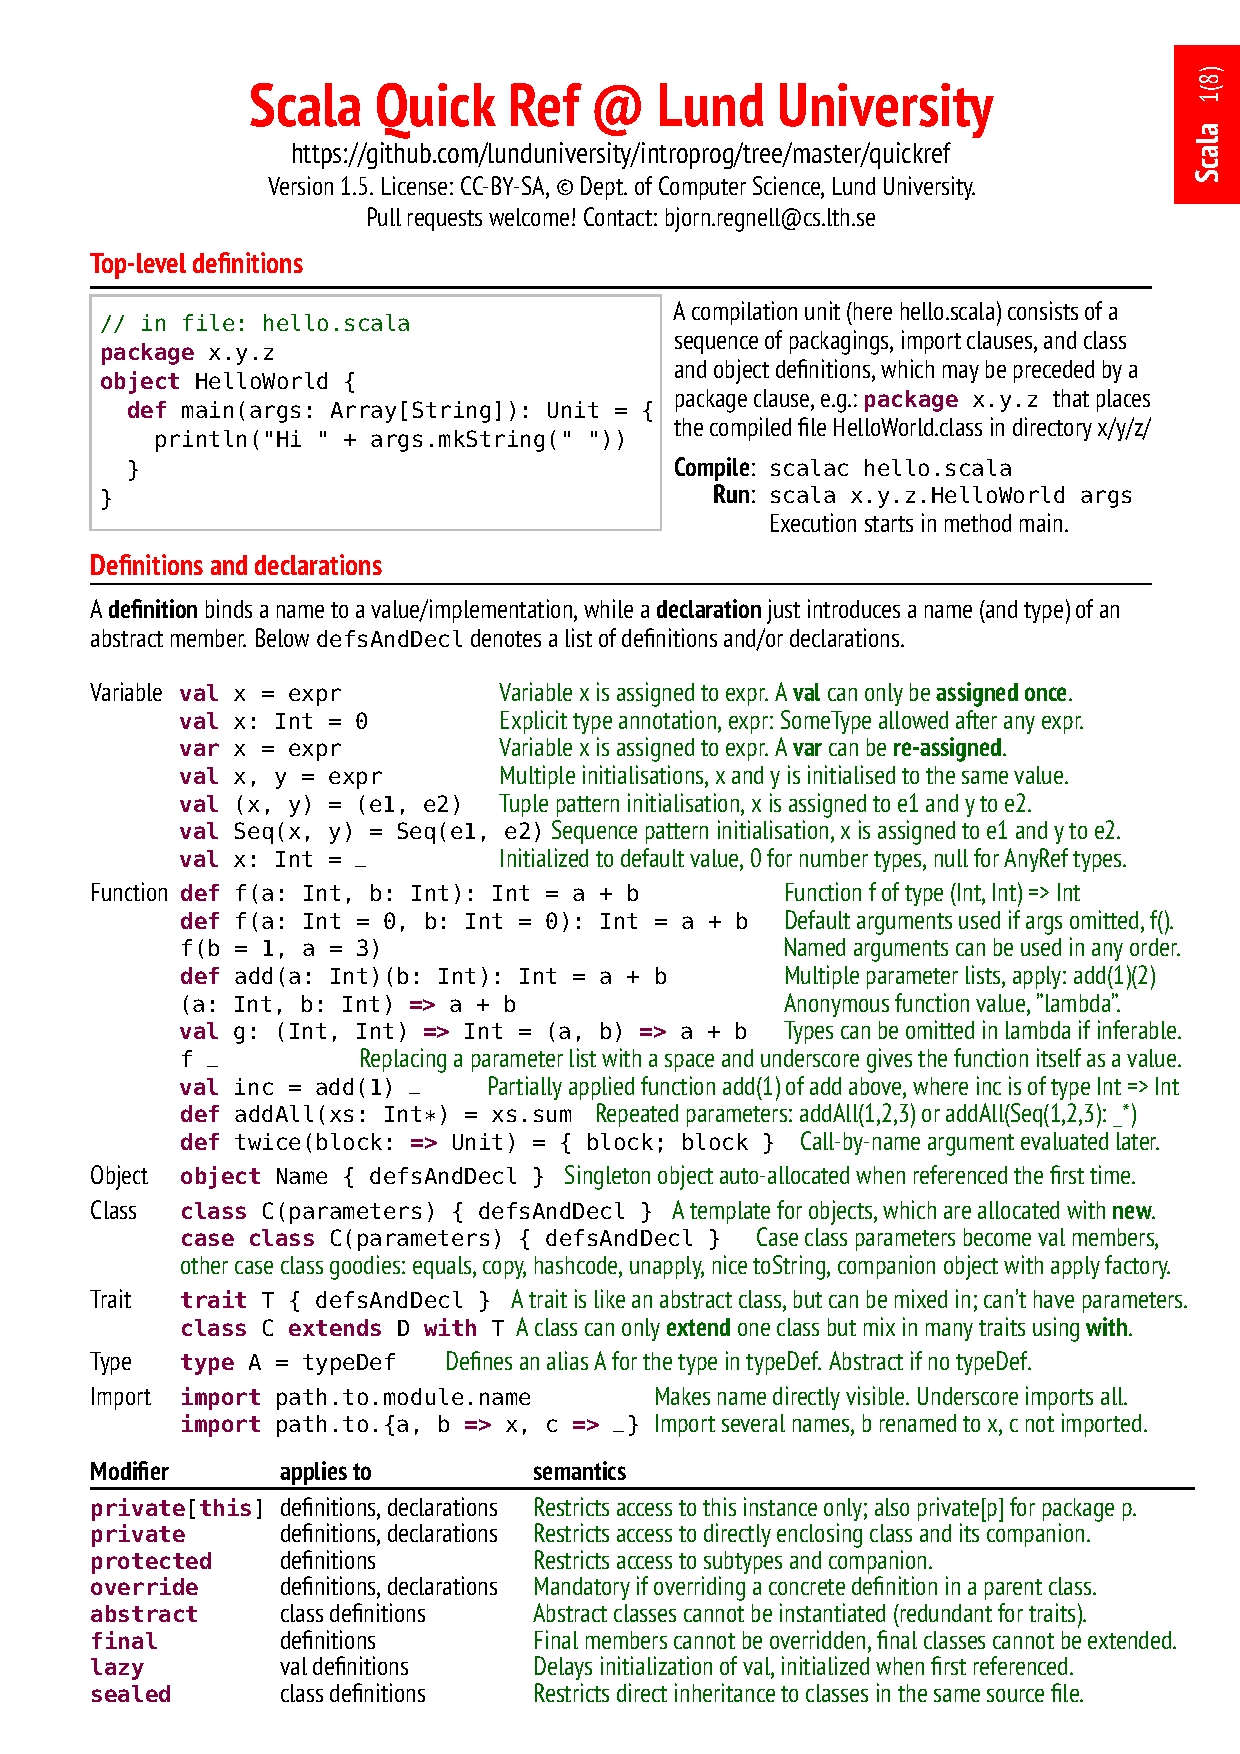
\includepdf[pages={1-12}, scale=0.77, frame]{../quickref/quickref.pdf}


\end{document}
